\documentclass[cn,11pt,twocol]{elegantbook-zh-tw}

\usepackage{blindtext}

\title{生物統計 (Biostatistics)}
\subtitle{課堂講義}

\author{施銘杰}
\institute{清華大學學士後醫學系}
\date{\today}
% \version{0.01}

% \extrainfo{Far better an approximate answer to the right question, which is often vague, than an exact answer to the wrong question, which can always be made precise. --- J. Tukey}

\extrainfo{}

\logo{NTHU.png}
\cover{cover.jpg}

\begin{document}
\maketitle
\tableofcontents
\mainmatter
\hypersetup{pageanchor=true}

\chapter{統計學概論}
    在這個資料取得越來越容易的時代,各個領域都希望能夠分析手上的資料、獲得結論並進行決策。例如在醫療領域中,我們常想知道一個療法對於病患的預後是否有影響,以進行後續補助政策的制定或治療指引的撰寫;或是能不能夠利用病患的影像資料、抽血資料和病史預測疾病的發生率,以達到提前篩檢、早期診斷、早期治療的目的。因此,如何有效率地整理資料、去蕪存菁、並進行合乎科學原理的分析便變成為一門顯學。統計便是一門利用科學方法來處理並分析資料的學科。當今因為資訊計算能力的超指數成長,分析整理資料的方法種類和複雜度也呈現爆炸性的增長,但這些方法的目的仍然是探尋資料內部隱含的資訊,因此背後仍然是以統計架構為基石。本課程前半段將著重統計觀念的建立,包含為什麼需要利用統計方法分析資料,以及推論統計的邏輯基礎。後半段則將介紹常用的統計檢定與迴歸方法,並輔以因果推論的理論框架介紹,以期了解如何針對有興趣的研究議題,選擇適當的統計模型並解讀分析結果。在本章,我們會簡介統計學的發展歷史,並帶出統計學的兩大分支:描述性和推論性統計。針對推論性統計,我們還會探討母體、抽樣和樣本的概念,以及這些概念如何融合到推論性統計的流程中。

\begin{introduction}[第 \thechapter 章學習目標]
    \item 描述性統計和推論性統計的目的
    \item 母體、樣本和抽樣的概念
    \item 推論性統計的流程與背後假設
    \item 統計推論的初步評讀
\end{introduction}

\section{統計的分支:敘述性統計}
    相較於其他領域,統計是一門十分近代才成型的學科,約十八世紀才開始發展。統計的英文是 \textit{statistics},拉丁字源為 \textit{statisticum},意謂「政府的」,因為統計最初是政府用來處理國家級資料(例如人口、經濟),以幫助管理國家的方法。首度將 \textit{statistics} 這個字引入英文的人據傳是蘇格蘭的 Sir John Sinclair (1754-1835)。他編纂了一本共有 22 集的 \textit{Statistical Account of Scotland},記錄了當時蘇格蘭當時的各式資料,包括地理、人口、農工生產等等,且紀錄內容並不限於數字。例如圖\ref{fig:john_sinclair}所示,書中內容記錄了其中一個地區的人口職業分佈,還提到當地的道路狀況。

\begin{figure}[htbp]
  \centering
  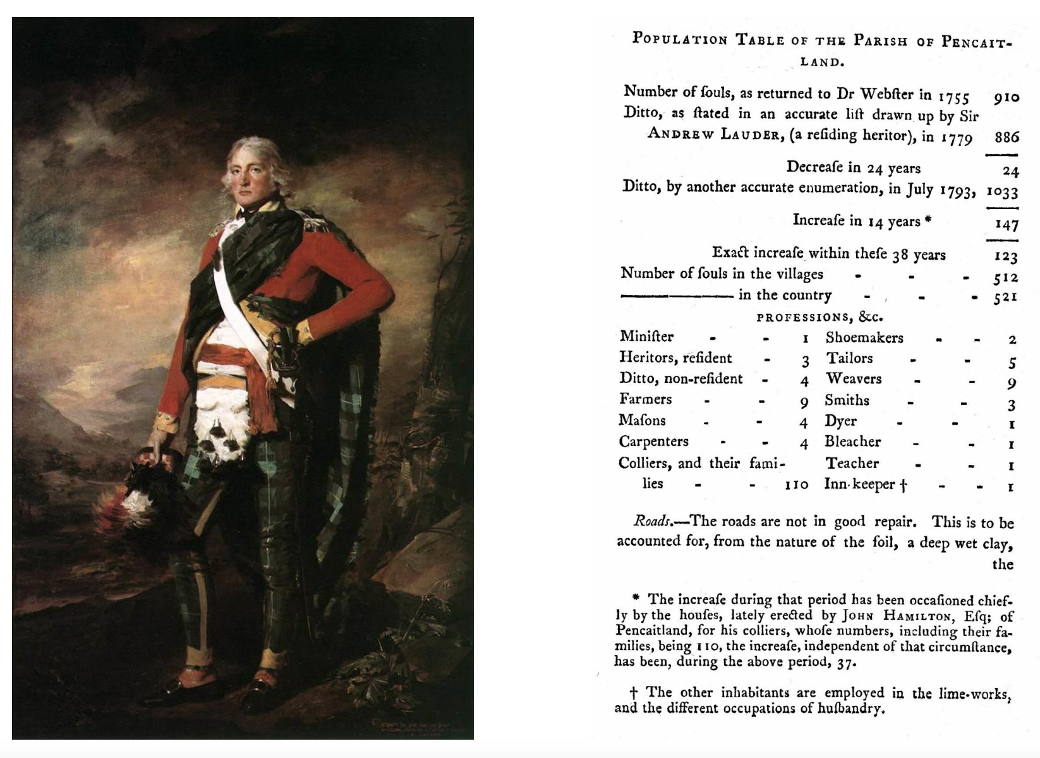
\includegraphics[width=0.9\textwidth]{figures/01-Overview/john_sinclair.png}
  \caption{Sir John Sinclair (1754-1835) 與 \textit{Statistical Account of Scotland} 的內頁}
  \label{fig:john_sinclair}
\end{figure}

    類似 \textit{Statistical Account of Scotland} 這類將資料整理後,以易懂的圖表呈現的方式一般被稱為\textit{描述性統計} (descriptive statistics)。描述統計學能將相對大量的資料精簡為具有代表性的統計數據(例如比例、平均值、中位數等描述統計量)或是圖片,以幫助我們快速了解資料的特性與隱含的訊息。運用得當的描述統計方法能夠讓決策者根據資料帶來的訊息即時地做出決策。例如,1854 年倫敦蘇活區 (Soho) 霍亂大爆發。該時代對於霍亂的病原為何仍然莫衷一是,但內科醫師 John Snow (1813-1858) 猜想霍亂的病原可能來自於水,因此根據蘇活區霍亂病例在家戶的分布做了圖 \ref{fig:john_snow},其中同一家戶的病例數越多,長條圖就越長。John Snow 發現霍亂病例似乎有以圖中的紅點為中心群聚分佈的趨勢,而該紅點標記的是蘇活區的一個公用抽水幫浦,和 John Snow 猜想的水媒傳染相符合。當地市政府而後也決定將抽水幫浦的手柄移除。John Snow 則因一系列霍亂相關的研究而被譽為「流行病學之父」。從這個圖片可以看出,John Snow將病例用散佈圖的方式標記是明智之舉。如果單純調查各分區的病例數而未作圖,則不見得能發現地理位置的群聚現象。

    \begin{figure}[htbp]
      \centering
      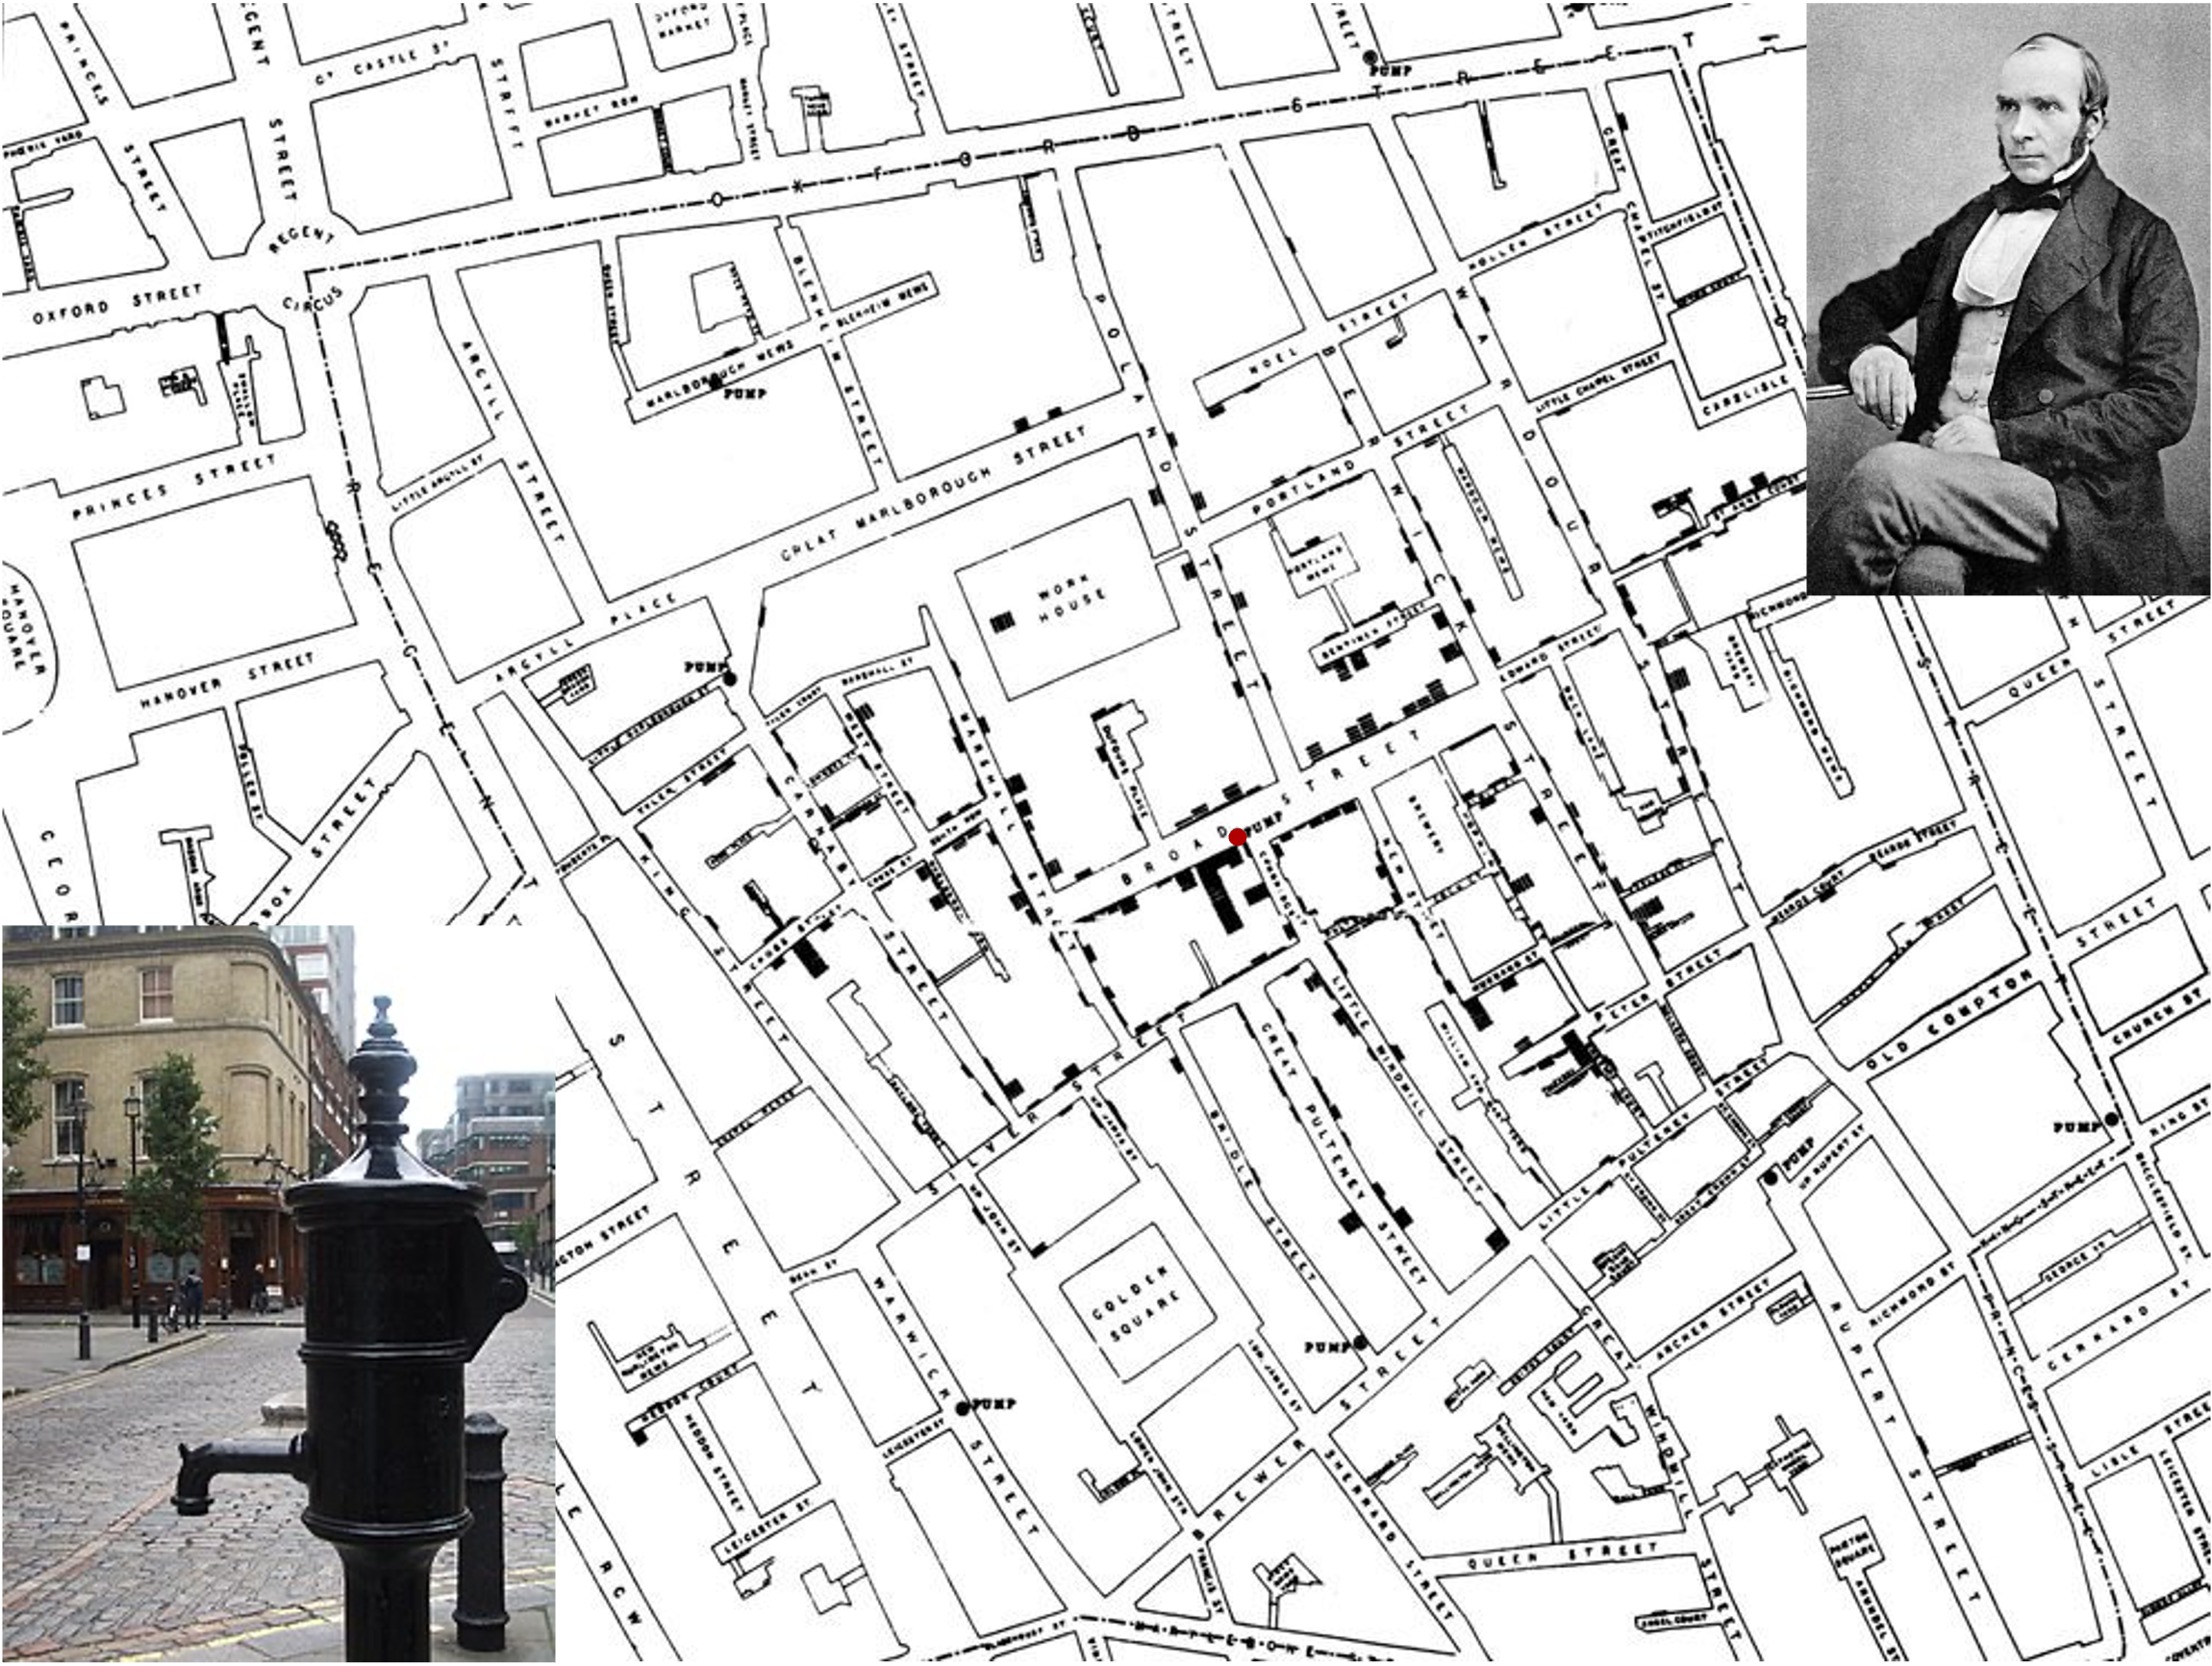
\includegraphics[width=0.9\textwidth]{figures/01-Overview/john_snow.png}
      \caption{John Snow (1813-1858)、其繪製的霍亂地圖、及地圖中心的公用抽水幫浦}
      \label{fig:john_snow}
    \end{figure}
    
    \bigskip
    
    \begin{custom}{思考}
        從 John Snow 繪製的圖片,是否已經足夠證明水就是霍亂的傳播根源?後來市政府將抽水幫浦的手柄移除,同時間霍亂疫情也逐漸緩和,如此是否已經足夠證明水就是霍亂的傳播根源?
    \end{custom}
    
    \bigskip
    
\section{統計的分支:推論性統計}

    有了描述統計學後,決策者理論上即可根據圖像或描述統計量來做決策。例如,利用健保資料庫了解國人糖尿病的患病率後,即可用患病率這個描述統計量估算糖尿病相關照護計畫的預算。然而,很多時候因為資源的限制,我們沒有辦法針對有興趣的目標量取得所有的資料。例如,如果我們有一個針對小細胞肺癌的新藥,並想要了解當前台灣第三期肺癌的病人服用該藥的副作用發生率(我們簡寫為 $p$)如何。理想上,我們想要搜集所有第三期肺癌的病人,都給予新藥後,評估出現副作用的比例。然而,這樣的作法在金錢資源上和倫理上都行不通。
    
    針對這個問題,一個可行的替代方法是,我們可以募集 $50$ 位第三期肺癌的病人,並給予新藥後,評估這 $50$ 位病人出現副作用發生率。比方說有 $2$ 位出現副作用,因此這群病人的副作用發生率為 $4\%$。只要我們募集的病人具有代表性,那麼「當前台灣第三期肺癌病人」的副作用發生率 $p$ 應該會和這群病人類似,大約是 $4\%$。然而,$p$ 顯然不太可能剛剛好是 $4\%$,因為這個算出來的 $4\%$ 會隨著募集到的病患不同而變動:如果重新募集另外兩組 $50$ 位病人,發生副作用的人數可能因為隨機性而變成 $1$ 人或 $3$ 人,進而算得 $2\%$ 或 $6\%$ 的發生率。因此,我們只知道 $p$ 應該在 $4\%$ 左右,但是它的實際數值則因為隨機的變動而有不確定性。因此,統計學家引進了數學的機率論來描述並處理不確定性,因而衍生出\textit{推論性統計}(Inferential statistics)。
    
    在推論性統計中,有幾個名詞是我們必須需要熟悉的。我們條列如下,並以上述例子作為對照:

    \begin{itemize}
        \item \textit{母體} (Population):我們實際上有興趣的總群體,「當前台灣第三期肺癌的病人」。
        \item \textit{參數} (Parameter):我們有興趣的目標量,「肺癌病人接受新藥的副作用發生率 $p$」。
        \item \textit{抽樣} (Sampling):從母體抽取一部份個體的過程。
        \item \textit{樣本} (Sample):從母體抽出的個體,「$50$ 人的第三期肺癌病人」。
        \item \textit{樣本數} (Sample size):樣本的個體數,「$50$」。
        \item \textit{參數估計式} (Parameter estimator):根據我們對母體的假設及抽樣方法,建構出一個估計參數的方法,「樣本中發生副作用的人數除以樣本數」。
        \item \textit{參數估計量} (Parameter estimate):把樣本帶入參數估計式得到的數值,「$4\%$」。
    \end{itemize}

    隨後,根據圖\ref{fig:flowchart}的流程,我們可以利用推論性統計的技巧,根據抽樣方法和母體假設對參數做推論,例如「當前台灣第三期肺癌病人服用新藥的副作用發生率 $95\%$ 信賴區間為 $(0.49\% - 13.71\%)$」或「在 $5\%$ 的顯著水準下,沒有足夠證據顯示當前台灣第三期肺癌病人服用新藥的副作用發生率大於 $1\%$」等等。以上的推論現在看起來可能不知所云,但後續課程將詳細介紹推論性統計的解讀方法,而後我們就會知道這些推論背後的意義,以及為什麼要弄得那麼複雜。
    
    圖\ref{fig:flowchart}的流程也給我們一個檢視統計推論中每個環節是否正確的藍圖。例如,針對公共議題的民意調查,如果只在火車站或夜市附近作隨機街訪,則樣本來源都只來自活動於火車站或夜市附近的居民,因而可能無法我們預想的「全民」母體。針對心血管疾病發病率的預測模型,如果建模資料來自於高階健檢的檢查資料,則該預測模型可能無法外推到全國國民使用。進行氣喘急性發作危險因子的分析時,如果單一病患因多次發作而提供多筆資料,但是使用的分析方法卻假設抽樣得到的樣本是互不相關,那麼得到的推論結果就會有偏誤。而且我們可以看到,推論統計中數學能夠做的只是根據母體假設以及抽樣方法儘量建構好的參數估計方法,但如果母體假設有誤或抽樣流程不正確,那麼統計能夠幫忙的程度就非常有限。
    
    \begin{figure}[htbp]
      \centering
      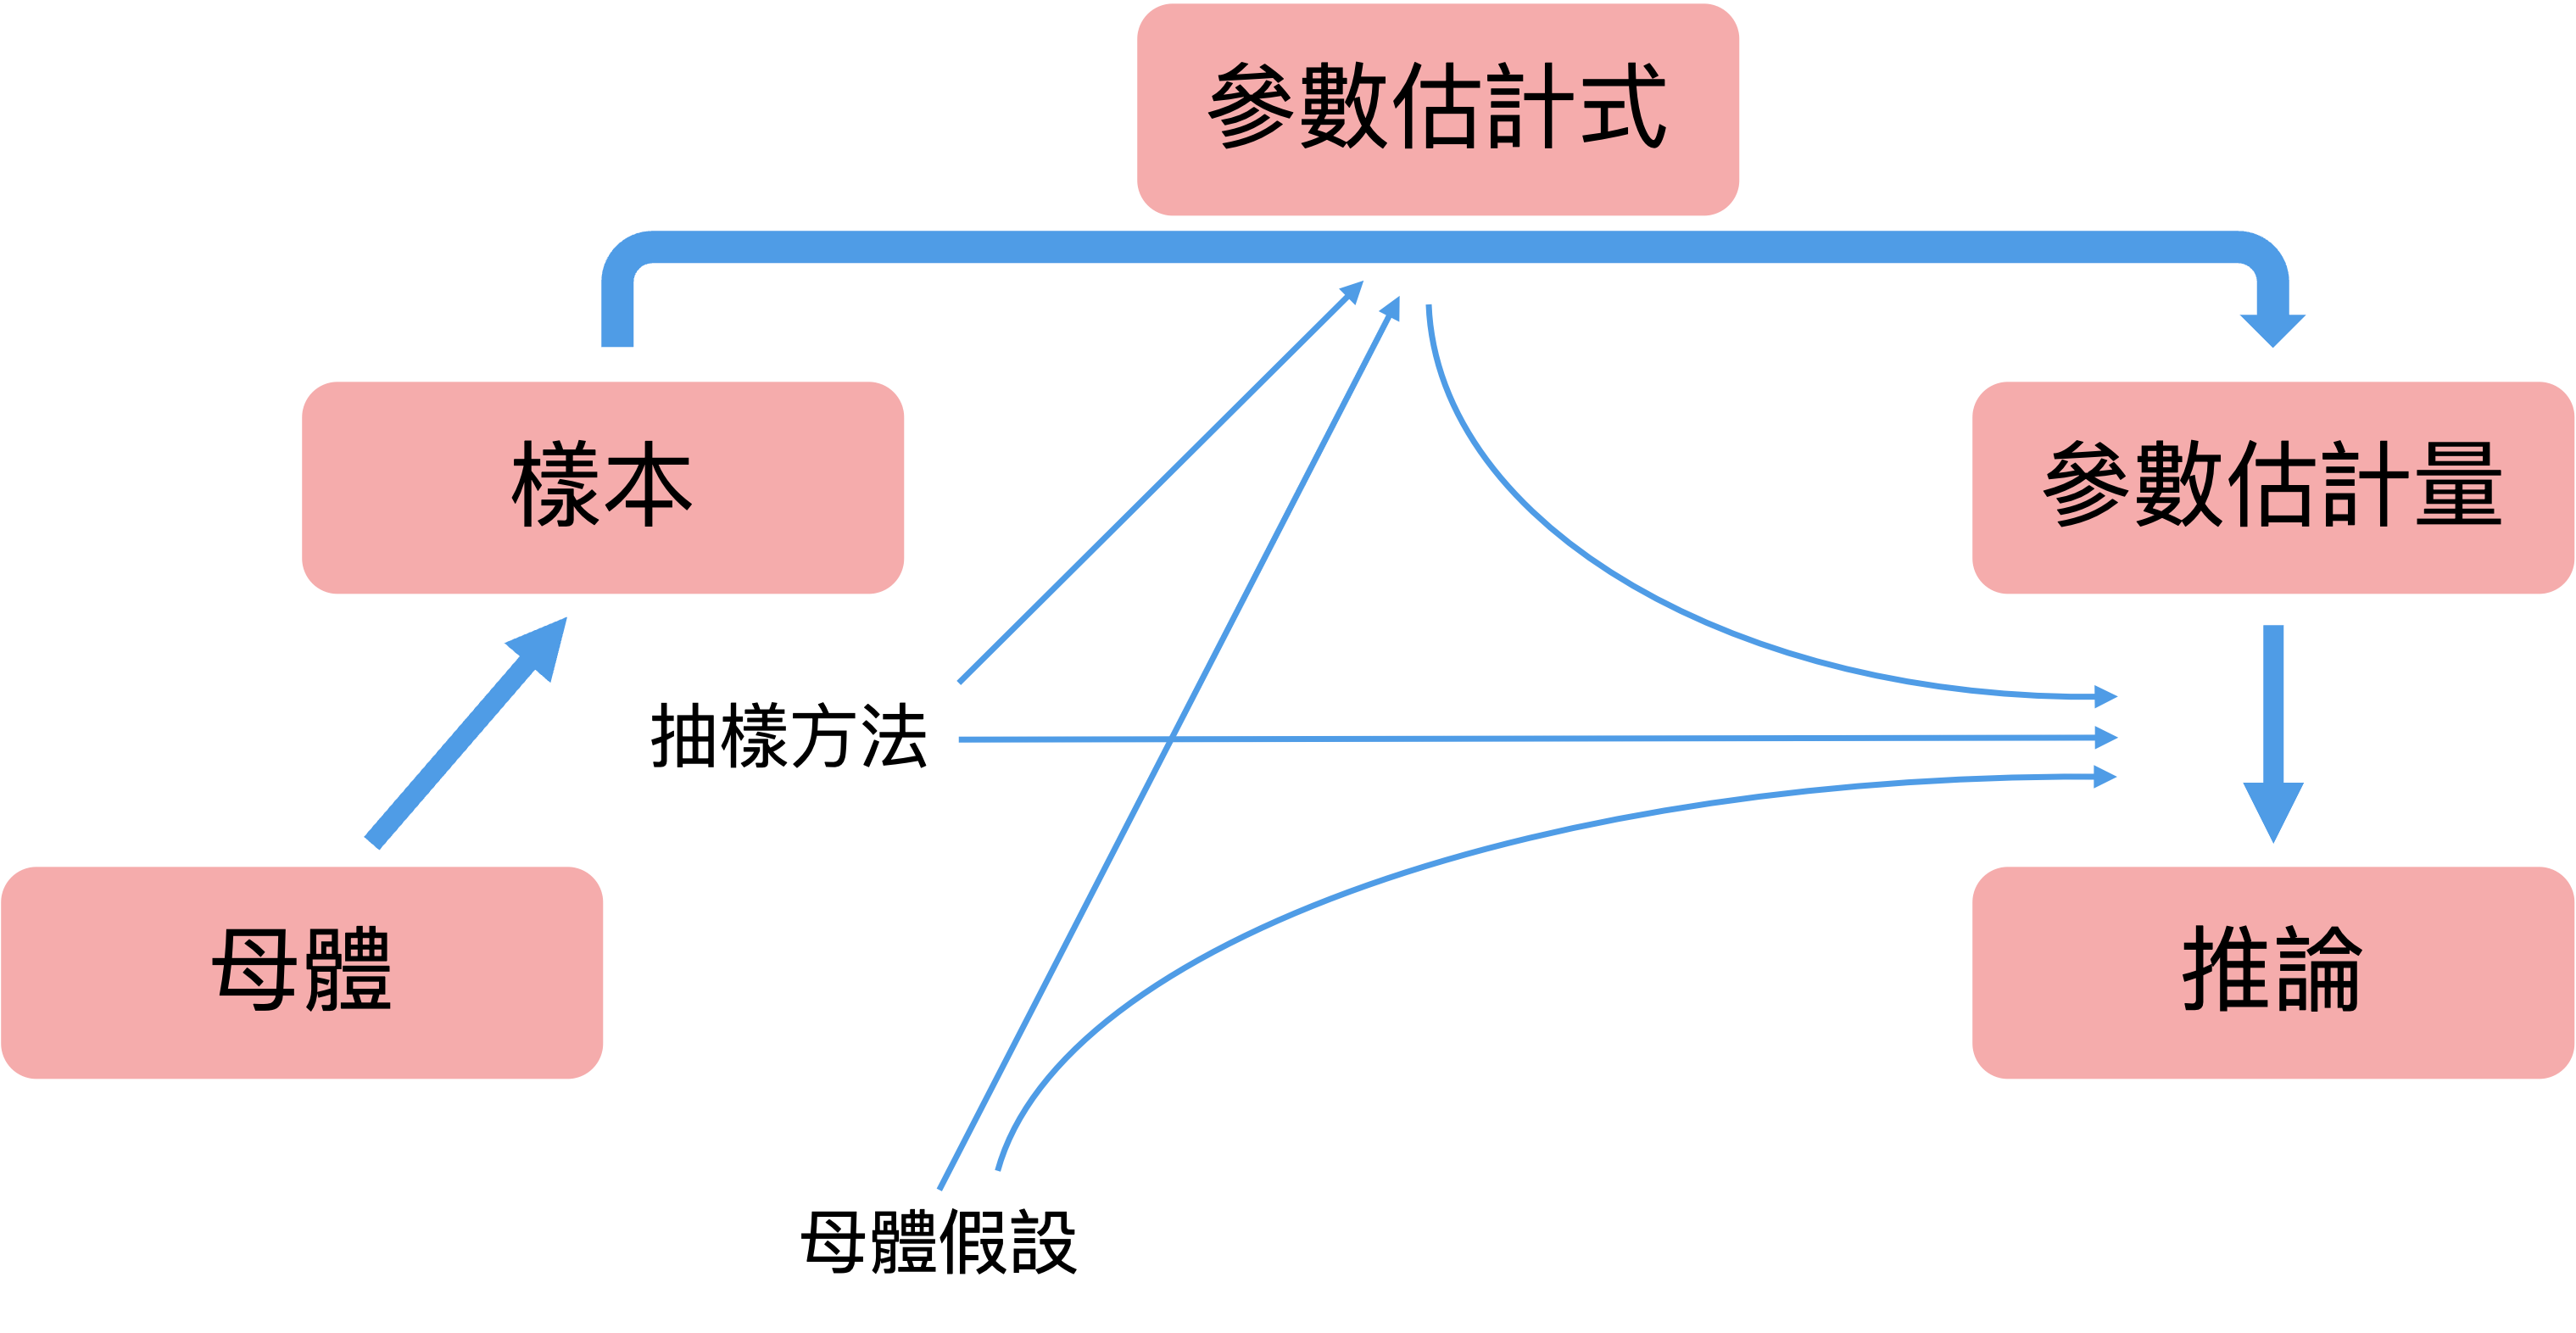
\includegraphics[width=0.9\textwidth]{figures/01-Overview/flowchart.png}
      \caption{推論統計的流程架構}
      \label{fig:flowchart}
    \end{figure}
    
    \bigskip
    
    \begin{custom}{思考}
        現今健保資料庫的覆蓋率已經超過 99.7\%。如果以台灣民眾為母體,那麼健保資料庫等同幾乎收集了母體的所有資料。在這個情況下,還有推論統計的必要嗎?
    \end{custom}
    
    \bigskip
    
    \begin{custom}{思考}
        在問卷調查中(例如:調查對某政策的支持與否),經常會出現某些題目漏答或拒答的現象。此時如果是以下的假設情境,是不是能夠用有回答的問卷估計出正確的政策支持率?(1) 漏(拒)答是完全隨機的,和受訪者的任何特性均無關;(2) 漏(拒)答不是完全隨機的,且和受訪者支不支持政策有關;(3) 漏(拒)答並非完全隨機,但僅和受訪者的性別、年齡有關,且問卷中有詢問性別及年齡;(4) 漏(拒)答並非完全隨機,但僅和受訪者的教育程度有關,但問卷未詢問教育程度。
    \end{custom}
    
\section{統計學的獨立發展}

    統計學的雛型雖然從十八世紀萌芽,並接受數學機率論的薰陶而逐漸茁壯,但直到十九世紀末,統計學才作為一門獨立、有系統性的學門發展。其中最重要的推手是研究遺傳學的 Francis Galton (1822-1911) 以及他的門生 Karl Pearson (1857-1936)。Galton 受到他的堂哥、也是遺傳學家的 Charles Darwin 的影響,對於連續性狀如身高、智力的遺傳感興趣。Galton 試圖用數學模型來分析並描述這些性狀的遺傳特性,因而發展出了回歸、相關性等等統計學最基本的概念。Pearson 作為 Galton 的門生(及被贊助者),完善了回歸及相關性的數學架構,並提出了假設檢定、卡方檢定、主成分分析等等統計方法與工具。而後,Ronald Fisher (1890-1962) 大力推進了遺傳以及推論統計的數學理論,並基於農業研究提出實驗設計法以及其統計分析,如變異數分析 (analysis of variance)。Galton、Pearson 和 Fisher 三人為當代推論性統計打下了重要基礎。
    
    \begin{figure}[htbp]
      \centering
      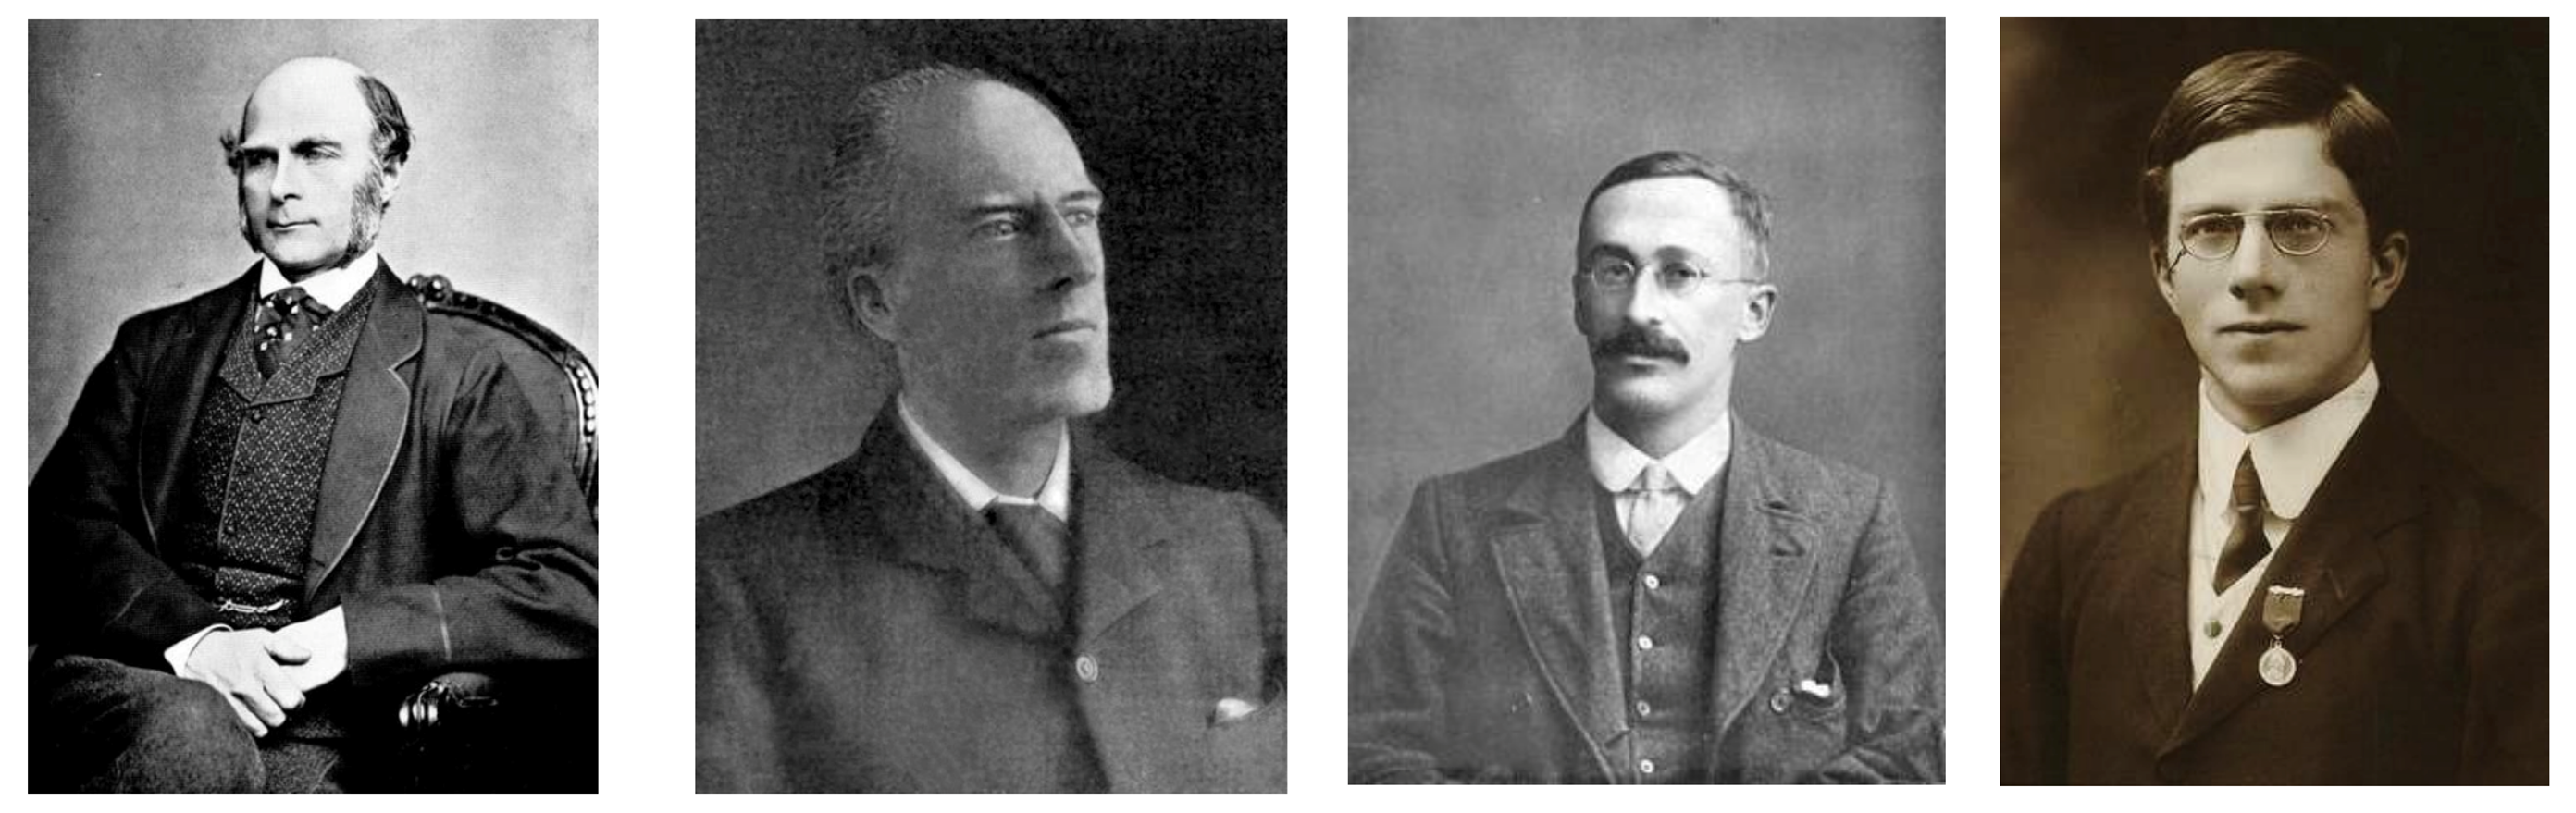
\includegraphics[width=0.9\textwidth]{figures/01-Overview/statisticians.png}
      \caption{奠基統計學的統計學家:(左至右)Francis Galton, Karl Pearson, William Gosset, Ronald Fisher}
      \label{fig:statisticians}
    \end{figure}
\chapter{資料型態與描述性統計}
    在資料分析及統計推論前,我們經常需要先對資料有初步的認識,從而決定是否要先對資料做前處理(例如轉換、合併、處理離群值等等),以及應該用什麼統計方法進行分析。當資料量不大的時候,我們可以將資料全部列出來檢視,但隨著資料量的增大,我們就需要依賴描述性統計提取資料的特徵。本章我們將認識生醫資料常見的變數型態,針對這些變數型態有哪些適用的描述性統計量和圖表,以及這些描述性統計量和圖表的基本性質。
    
    \begin{introduction}[第 \thechapter 章學習目標]
        \item 生醫資料的變數常見型態
        \item 常見的描述性統計量和圖表及適用的變數型態
        \item 資料線性轉換對平均值、變異數、標準差的影響
    \end{introduction}

\section{生醫資料中變數的常見型態}

    一般生物醫學資料最常見的格式如下表:

    \begin{table}[htbp]
        \begin{center}
            \begin{tabular}{cccccccc}
                \toprule
                年齡 & 性別 & 教育程度 & 居住地 & 身高 & 體重 & 一年癲癇發作次數 & $\cdots$\\
                \hline
                30 & 男 & 高中(職) & 北北基 & 160 & 53.3 & 3 & $\vdots$ \\
                27 & 女 & 大專 & 中彰投 & 153 & 42.6 & 0 & $\vdots$ \\
                31 & 男 & 國中以下 & 桃竹苗 & 182 & 84.2 & 2 & $\vdots$ \\
                $\vdots$ & $\vdots$ & $\vdots$ & $\vdots$ & $\vdots$ & $\vdots$ & $\vdots$ & $\vdots$ \\
                \bottomrule
            \end{tabular}
            \caption{常見資料格式\label{tab:data}}
        \end{center}
    \end{table}
        
    其中每一個 row(橫列,但不同國家的行列定義不同,因此我們這裡通稱 row)代表一筆資料,也常被稱為一個\textit{觀察值} (observation)。每個 column(直行)則代表不同的測量標的,該標的也被稱為\textit{變數}或\textit{變項} (variable)。從表\ref{tab:data}可以看出,各變項依據其可能的取值可粗略分為兩種:一種是以類別名稱取值的\textit{類別型變項} (categorical variable),例如性別、教育程度、居住地;另一種則是以有實際意義的數字取值的\textit{數值型變項} (numerical variable),例如年齡、身高、癲癇發作次數。類別型變項的各種類別取值也被稱為\textit{層次} (level)。在實務上,為了節省資料存儲空間以及減少錯誤,類別型變項的取值常會被替換為整數的數字,例如性別為男取值 1、女取值 0,或是教育程度國中以下、高中(職)、大專、碩士、博士分別替換為0、1、2、3、4。替換的數字與層次實際名稱的對照表則存儲在編碼冊 (coding book) 中,如表\ref{tab:data_coding}所示。

    \newpage

    \begin{table}[htbp]
        \begin{center}
            \begin{tabular}{cccccccc}
                \toprule
                年齡 & 性別 & 教育程度 & 居住地 & 身高 & 體重 & 一年癲癇發作次數 & $\cdots$\\
                \hline
                30 & 1 & 1 & 1 & 160 & 53.3 & 3 & $\vdots$ \\
                27 & 0 & 2 & 3 & 153 & 42.6 & 0 & $\vdots$ \\
                31 & 1 & 0 & 2 & 182 & 84.2 & 2 & $\vdots$ \\
                $\vdots$ & $\vdots$ & $\vdots$ & $\vdots$ & $\vdots$ & $\vdots$ & $\vdots$ & $\vdots$ \\
                \bottomrule
            \end{tabular}

            \bigskip

            \begin{tabular}{c|l}
                \toprule
                性別 & 女:0;男:1\\
                \hline
                教育程度 & 國中以下:0;高中(職):1;大專:2;碩士:3;博士:4\\
                \hline
                \multirow{2}{*}{居住地} & 北北基:1;桃竹苗:2;中彰投:3;\\
                & 雲嘉南:4;高屏:5;宜花東:6;外島:7\\
                \bottomrule
            \end{tabular}
            \caption{常見編碼資料格式與編碼冊\label{tab:data_coding}}
        \end{center}
    \end{table}

    根據類別型變項和數字型變項的特性,我們還可以再將它們細分:

    \begin{itemize}
        \item 類別型變項
        \begin{itemize}
            \item \textit{名目} (Nominal):各層次間沒有排序關係的類別型變項,例如性別、居住地。
            \begin{itemize}
                \item \textit{二元} (Binary):僅有兩個層次的名目變項。為了後續分析方便,通常會把其中一個層次編碼為0,另一個層次編碼為1。
                \item \textit{多元} (Multinomial):有三個以上層次的名目變項。
            \end{itemize}
            \item \textit{有序} (Ordinal):各層次間有排序關係的類別型變項,例如教育程度、收入區間。為了後續分析方便,編碼通常會按照排序關係以遞增的整數編碼,如表\ref{tab:data_coding}的教育程度編碼。
        \end{itemize}
        \item 數值型變項
        \begin{itemize}
            \item \textit{計數} (Count):取值為非負的整數,例如一年內癲癇發生次數、牙齒剩餘顆數。
            \item \textit{連續} (Continuous):實務上如果取值不連續但是可能數值足夠多(例如身高均以整數紀錄、因此可能取值有限),常常也視為連續。
            \begin{itemize}
                \item \textit{等距} (Interval):變項取值的零點是人為的,因此兩個數值相除的意義不大。例如智商、pH 值。
                \item \textit{等比} (Ratio):變項取值有一個有意義的零點,使得兩個數值相除有意義。例如身高、體重。
            \end{itemize}
        \end{itemize}
    \end{itemize}

    \begin{custom}{思考}
        根據這個定義,攝氏溫度、華氏溫度和克式溫度(Kelvin scale)應該是哪種資料型態?如果一個問卷的題目讓填答者填1到5分的(整數)滿意度,那麼這個題目的答案應該是哪種資料型態?如果疼痛指數是1到10分的整數,那麼它應該是哪種資料型態?
    \end{custom}

    \begin{custom}{思考}
        如果資料是一張 X 光片,那麼我們還能把圖像轉成數值型態嗎?更進一步,如果圖像不是黑白的,那麼要怎麼轉成數值型態?
    \end{custom}

    \begin{custom}{思考}
        一般來說,資料中的每一個 row 通常代表一筆資料,而不同的 row 通常預設是由不同的病患所貢獻。如果我們現在追蹤一群高血壓病患十年,每三個月追蹤一次(共四十次),並想記錄他們追蹤起始年齡、性別、高血壓家族史及每次追蹤的收縮壓和舒張壓,那麼應該如何記錄資料?
    \end{custom}

    了解變項的資料型態後,我們就可以進一步探討如何選擇並計算描述性統計量,來描述變項的特徵。描述性統計量本質上還是一個參數估計量(請參見第一章),而且是用來估計母體描述性參數的估計量。因此我們要先探討針對各種資料型態的母體,有哪些適用的描述性參數,以及如何用樣本計算出描述性統計量來估計這些參數。
    
\section{類別變項的描述性統計量與圖表}

    對於類別變項最具描述性的參數,即為\textit{各層次的出現比例}(由於類別變項各層次對應的編碼只是人為設定,所以一般來說,母體的描述性參數不會牽涉到這些編碼的數值。)。而估計這些比例的描述性統計量也很好計算,只要計算各層次在樣本中出現的比例即可。舉例而言,假設表\ref{tab:data}是從全台灣癲癇病患中隨機抽取 250 位所得到的資料,而我們現在關注的是「教育程度」這個變項。居住地的層次總共有五個:國中以下、高中(職)、大專、碩士、博士。因此,針對教育程度變項的母體描述性參數,即為台灣癲癇病患教育程度分別為這五個層次的比例(注意到這五個比例的總和為一,所以只要知道其中四個就可以推得最後一個)。其相對應的描述性統計量就是 250 位抽中的病患中,各類教育程度的比例。這些資訊常整理如表\ref{tab:categorical_desc},其中人數為實際觀察到的層次觀察個數,也被稱為\textit{頻率} (frequency),而比例則是這些頻率的相對大小,所以也被稱為\textit{相對頻率} (relative frequency)。

    \begin{table}[htbp]
        \begin{center}
            \begin{tabular}{lrl}
                \toprule
                \textbf{教育程度} & \textbf{人數} & \textbf{(比例\%)}\\
                \hline
                國中以下 & 52 & (20.8)\\
                高中(職) & 60 & (24.0)\\
                大專 & 112 & (44.8)\\
                碩士 & 23 & (9.2)\\
                博士 & 3 & (1.2)\\
                \bottomrule
            \end{tabular}
            \caption{類別變項的頻率與相對頻率表\label{tab:categorical_desc}}
        \end{center}
    \end{table}

    表\ref{tab:categorical_desc}也可以用圖呈現。最簡單的方法是如圖\ref{fig:barplot}的\textit{長條圖} (barplot),其中左圖是用頻率做為縱軸,右圖是用相對頻率做為縱軸,橫軸則均標示各個層次的標籤。長條圖橫軸層次順序不影響圖片的正確性,但因教育程度是有序變項,所以在圖\ref{fig:barplot}中我們採用教育程度由左而右由低到高的排列,以增加直觀性。
    
    \begin{figure}[htbp]
      \centering
      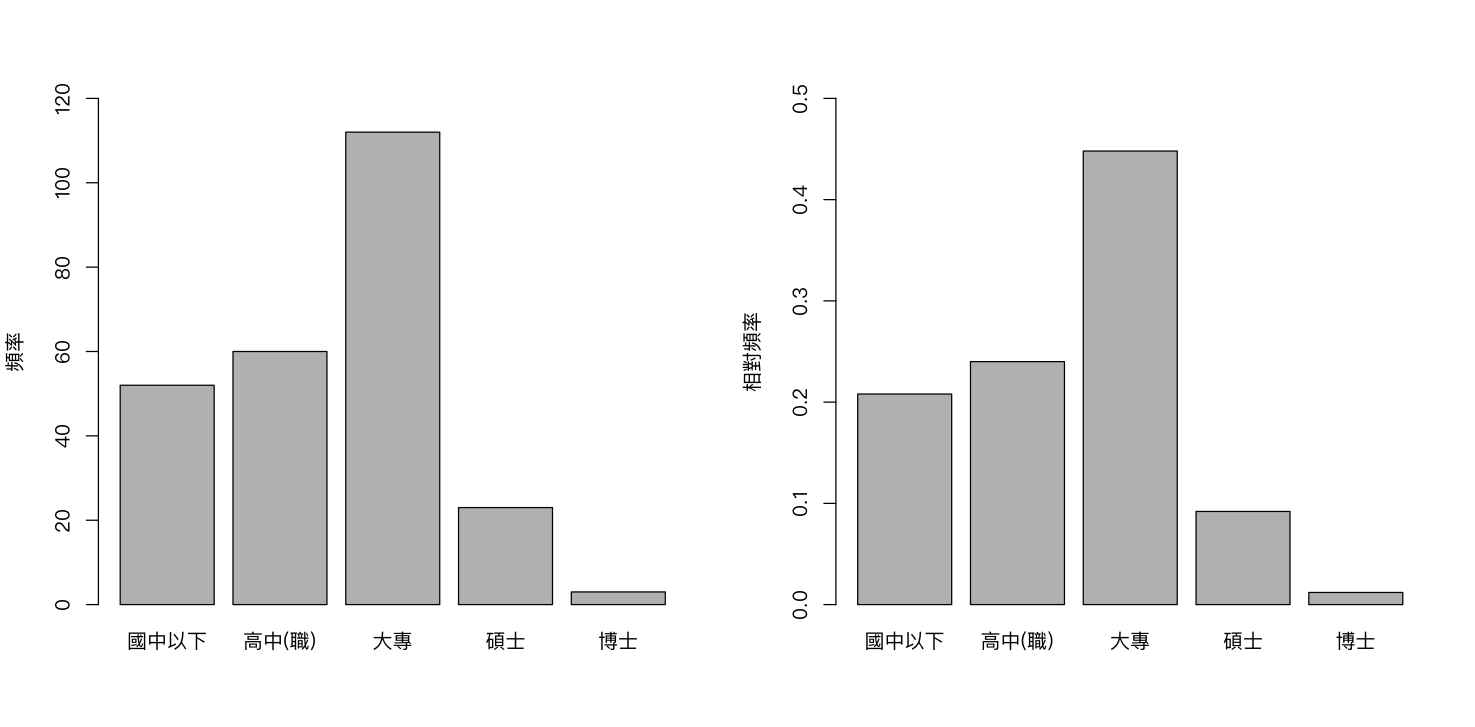
\includegraphics[width=\textwidth]{figures/02-Descriptive_statistics/barplot.png}
      \caption{以頻率與相對頻率作縱軸的長條圖}
      \label{fig:barplot}
    \end{figure}

    圖\ref{fig:pareto_chart_pie_chart}的左方是由長條圖衍生出的\textit{帕雷托圖} (Pareto chart)。其特點為層次由左而右按照頻率排列,因此靠左的層次代表佔總體的比例較大。另外,除了對應左縱軸頻率的直條圖以外,帕雷托圖還增加了一個折線圖,對應到右縱軸的\textit{累積比例} (cumulative percentage)。累積比例代表該層次及其左側的所有層次的總比例,例如國中以下的累積比例為大專的比例44.8\% + 高中(職)的比例 24.0\% + 國中以下的比例 20.8\%,總和為 89.6\%。繪製累積比例的好處在於,讀者可以輕易看出該變項是否主要由特定一群層次所組成,以及其所佔比例,例如大專和高中(職)畢業的病患大約佔了總體 70\%。圖\ref{fig:pareto_chart_pie_chart}的右方則是常見的\textit{圓餅圖} (pie chart)。除非層次的佔比很懸殊,否則圓餅圖很難直觀表現出層次佔比的差異(例如國中以下和高中(職)的佔比大小,單就圖而言很難分出來),所以通常不建議使用。\;\;\;\;\;\;\phantom{X}

    \begin{figure}[htbp]
      \centering
      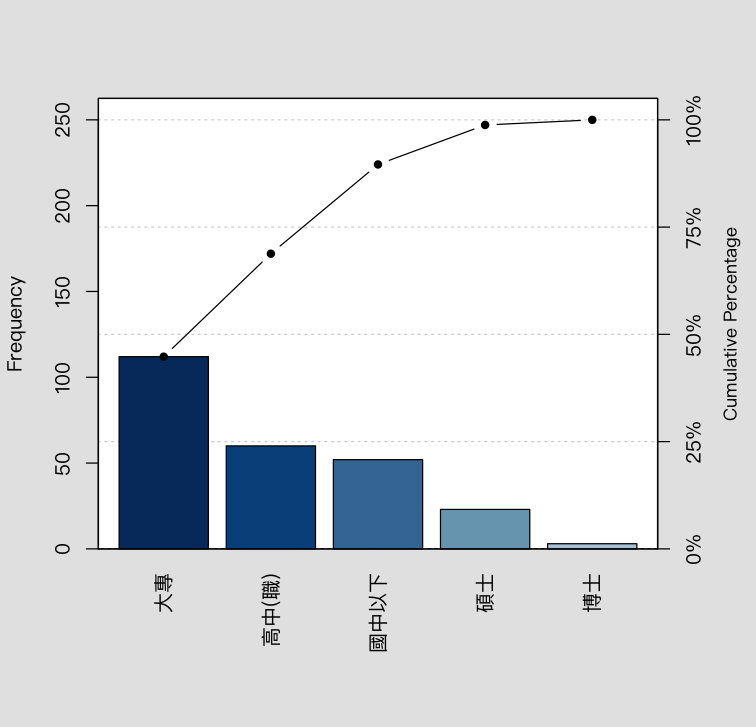
\includegraphics[width=0.48\textwidth]{figures/02-Descriptive_statistics/pareto_chart.png}
      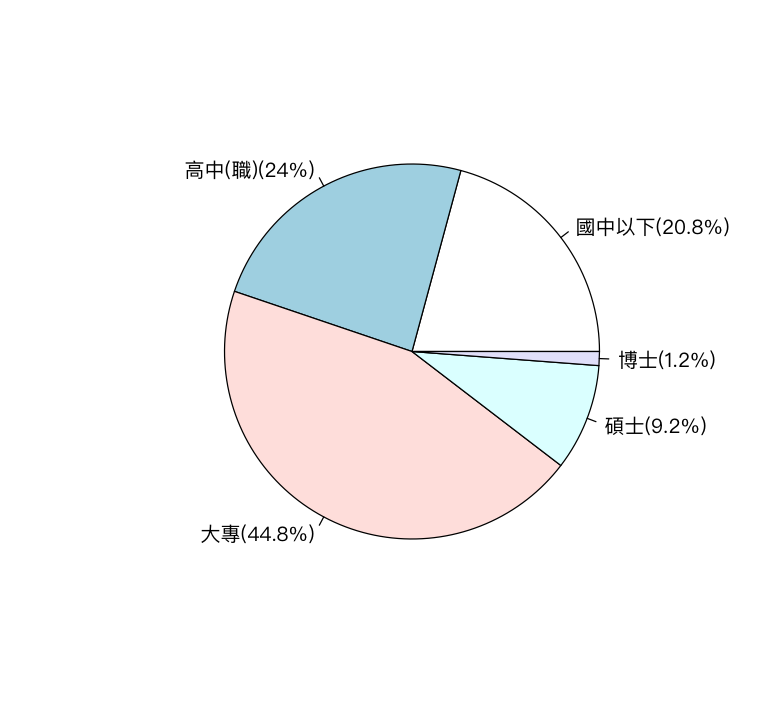
\includegraphics[width=0.48\textwidth]{figures/02-Descriptive_statistics/pie_chart.png}
      \caption{帕雷托圖與圓餅圖}
      \label{fig:pareto_chart_pie_chart}
    \end{figure}
    
    %我們從清華大學隨機抽取了 100 位大學生並記錄了「性別」這個變項。我們的母體是清華大學的所有大學生,而這些大學生的性別層次有兩個:男和女,所以針對性別變項的母體描述性參數即為「清華大學生的男生比例」及「清華大學生的女生比例」(因為加起來等於一,所以知道一個比例就可以推出另外一個)。相對應的描述性統計量就是 100 位抽中的大學生中,男性和女性的比例。

\section{數值變項的描述性統計量及圖表}
    和類別變項不同的是,數值變項的取值可能性多了許多,而且具有解釋意義。因此數值變項的母體描述性參數相對於類別變項更為多元。針對數值變項,我們能用\textit{直方圖} (histogram) 來視覺化母體的取值狀況,如圖\ref{fig:descriptive_cont}所示。繪製直方圖時,我們先將數值變項依可能取值切割成大小相等的區間,例如圖\ref{fig:descriptive_cont}中我們把取值區間以 0.5 的寬度分成$[10,10.5),[10.5,11),[11,11.5),...,[19.5,20)$,其中 $[a,b)$ 代表 $\ge a$ 但 $<b$ 的區間。而後即可計算落入各區間的觀察值個數並以直條繪製頻率或相對頻率。注意到直方圖和長條圖不同地方在於,直方圖的每個直條之間是\textbf{沒有}間隙的(除非有區間恰好沒有觀察值)、而且不能隨意交換順序,以表明直方圖的各直條代表連續且有序的組別。

    \bigskip
    
    \begin{custom}{思考}
        在製作直方圖時,如果區間寬度過大或過小,會對圖造成什麼影響?
    \end{custom}

    \bigskip

    \begin{figure}[htbp]
      \centering
      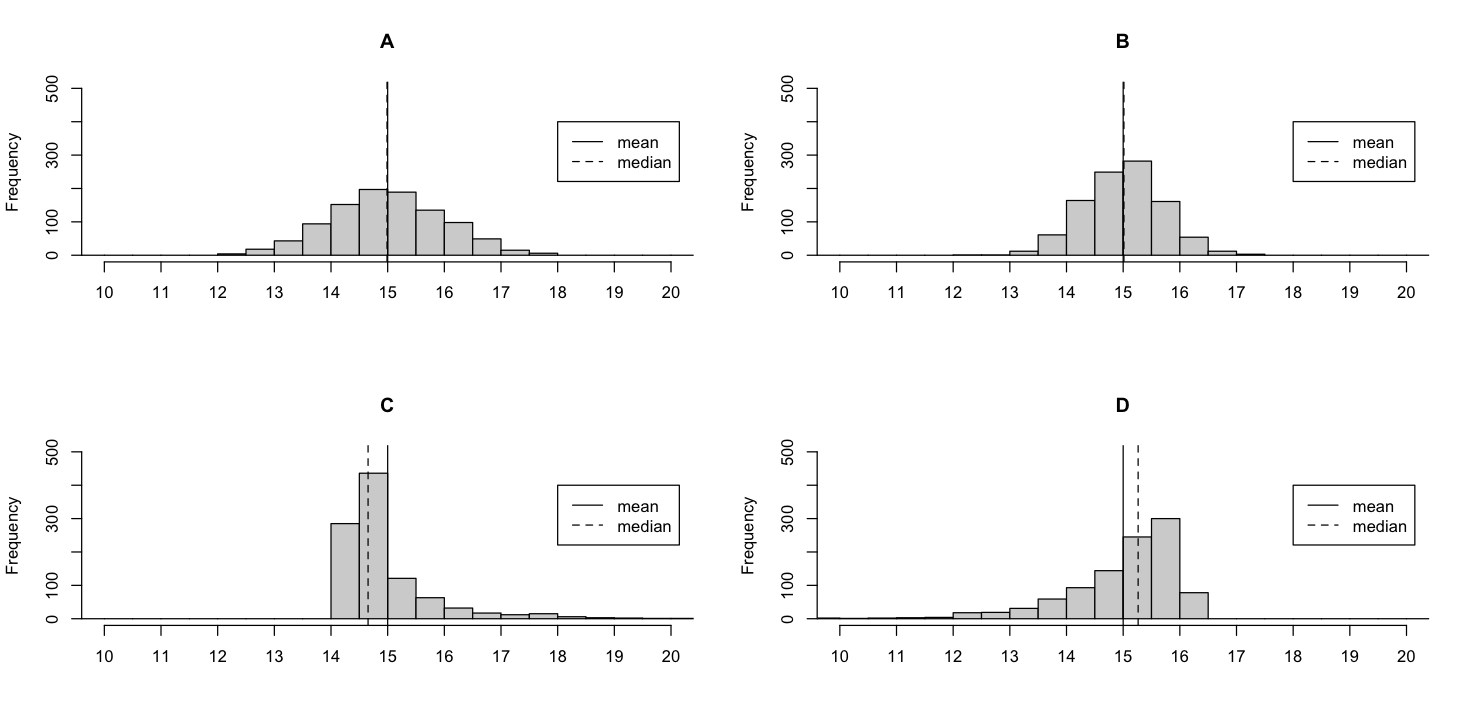
\includegraphics[width=\textwidth]{figures/02-Descriptive_statistics/descriptive_cont.png}
      \caption{四個不同母體的分布直方圖}
      \label{fig:descriptive_cont}
    \end{figure}

    \bigskip
        
    以下我們根據圖\ref{fig:descriptive_cont}討論一些常用的描述性參數。

\subsection{位置參數及其描述統計量}
    描述變項母體分佈的第一步,通常是找尋它的中心位置,我們才知道可能的取值大多會落在哪個數值附近。描述母體中心位置的參數通常被稱謂\textit{位置參數} (location parameter)。其中最常見的位置參數就是我們耳熟能詳的\textit{平均值} (mean),或是更精準的一點說,\textit{算術平均值} (population arithmetic mean)。假設變項 $X$ 的母體有 $N$ 個觀察值,分別為 $\tilde{X}_1, \tilde{X}_2, ... \tilde{X}_N$,則 $X$ 的\textit{母體平均} $\mu_X$ 的定義為:
    \[\mu_X = \frac{\tilde{X}_1+\tilde{X}_2+\cdots+\tilde{X}_N}{N} = \frac{1}{N}\sum_{i=1}^N \tilde{X}_i\]
    估計母體平均值的描述統計量被稱為\textit{樣本平均} (sample mean),常簡寫為 $\bar{X}$(唸作 X bar),假設樣本數為 $n$,觀察值分別為$X_1, X_2, ... X_n$,則樣本平均 $\bar{X}$ 的定義很直觀:
    \[\bar{X} = \frac{X_1+X_2+\cdots+X_n}{n} = \frac{1}{n}\sum_{i=1}^n X_i\]
    也就是把樣本觀察值全部加總取平均。注意到如果把變項做線性的放大平移 $X^* = aX+b$ ,也就是將放大$a$倍後加上$b$,那麼新的母體平均和樣本平均 $\mu_X^*$ 和 $s_X^2$ 會變成:
    \begin{align*}
        \mu_X^* &= \frac{(a\tilde{X}_1+b)+(a\tilde{X}_2+b)+\cdots+(a\tilde{X}_N+b)}{N}\\
        &= \frac{a(\tilde{X}_1+\tilde{X}_2+\cdots+\tilde{X}_N)+Nb}{N}\\
        &= a\frac{\tilde{X}_1+\tilde{X}_2+\cdots+\tilde{X}_N}{N} + \frac{Nb}{N} = a\mu_X + b\\
        \bar{X}^* &= \frac{(aX_1+b)+(aX_2+b)+\cdots+(aX_n+b)}{n}\\
        &= \frac{a(X_1+X_2+\cdots+X_n)+nb}{n}\\
        &= a\frac{X_1+X_2+\cdots+X_n}{n}+\frac{nb}{n}=a\bar{X}+b
    \end{align*}
    所以平均值同樣會以相同的倍率放大平移。
    
    平均值的算法雖然簡單,但是它的數值很容易受到極端的觀察值影響而偏移。例如在圖\ref{fig:descriptive_cont}的 C 中,雖然大於七成的母體取值都落在 14 到 15 之間,但母體平均值受到右方較大的數值影響而被往右拉到 15。此處以平均值 15 當作母體分布的「中心」似乎就不太合理。\textit{中位數} (median)是解決這個問題的一個替代方案,它的想法是把所有的取值由小排到大,並選取位置在正中間的數值。如果取值的數目為偶數,則取最中間兩個數值的平均。換句話說,如果把變項 $X$ 的母體觀察值由小排到大得到 $\tilde{X}_{(1)}, \tilde{X}_{(2)}, ..., \tilde{X}_{(N)}$,則母體中位數 $M_X$ 的定義為:
    \[M_X = \left\{\begin{array}{lr}
        \tilde{X}_{(\frac{N+1}{2})}, & N \text{是奇數}\\
        \frac{1}{2}\Big[\tilde{X}_{(\frac{N}{2})}+\tilde{X}_{(\frac{N}{2}+1)}\Big], & N \text{是偶數}
    \end{array}\right.\]
    估計母體中位數的描述性統計量即為\textit{樣本中位數} (sample median),其定義一樣很直觀:假設樣本觀察值由小排到大分別為$X_{(1)}, X_{(2)}, ... X_{(n)}$,則樣本中位數 $\hat{M}_X$ 為:
    \[\hat{M}_X = \left\{\begin{array}{lr}
        X_{(\frac{N+1}{2})}, & N \text{是奇數}\\
        \frac{1}{2}\Big[X_{(\frac{N}{2})}+X_{(\frac{N}{2}+1)}\Big], & N \text{是偶數}
    \end{array}\right.\]
    如前所述,中位數雖然常和平均值相去不遠,但是當變項的分布在一個方向有較多的極端值時,中位數就會和平均值有差距。如果極端值較常出現在右側,我們稱該分布為\textit{右偏} (right-skewed)或\textit{正偏} (positively skewed),此時一般而言,中位數會比平均值來得小(如圖\ref{fig:descriptive_cont}的C)。反之,如果極端值較常出現在左側,我們稱該分布為\textit{左偏} (left-skewed)或\textit{負偏} (negatively skewed),此時一般而言,中位數會比平均值來得大(如圖\ref{fig:descriptive_cont}的D)。
    
    雖然中位數雖然的確能夠直指分布的「中心」,但它的統計性質較為複雜,在後續很多的推論統計方法沒有辦法直接適用,因此一般而言我們還是會優先選擇平均值作為我們的位置參數以及描述統計量。另外一個可用的位置參數是 \textit{眾數} (mode),也就是所有觀察值中出現頻率最高的數值。不過在數值型變項,尤其是連續型變項中,各樣本取值的頻率常常都很低(例如一群人中,體重數值如果取到小數點後一位,那麼每種可能取值的出現次數可能都只有一次),所以實務上不常使用。

    \bigskip
    
    \begin{custom}{思考}
        如果某個變項在收集的過程中,已經先行將連續的變項分割為多個區間,並且記錄區間的頻率(例如 10-20 歲多少人、20-30 歲多少人、40-50 歲多少人),那麼我們還有辦法對該變項計算位置相關的描述統計量嗎?
    \end{custom}

\subsection{分散參數及其描述統計量}
    除了位置參數以外,我們看到 A 和 B 兩個變項的母體平均值和中位數均為 15 ,但是 B 的可能取值跨度明顯地比 A 還要小。換句話說,相對於 A,B 的取值比較常落在離平均值比較近的位置。用來描述這個分布特性的參數稱為分散參數 (dispersion parameter)。
    
    一個變項的取值和平均值之間的距離,如果平均而言較遠(例如圖\ref{fig:descriptive_cont}中的 A 有為數不少的取值跟平均值 15 的距離大於 1),那麼這個變項的分散程度應該比較大。因此,直覺上分散參數的定義可以用「取值和平均值的平均距離」來定義。如此定義的分散參數稱為\textit{平均絕對離差} (mean absolute deviation),也就是:
    \[\text{MAD}_X = \frac{|\tilde{X}_1-\mu_X|+|\tilde{X}_2-\mu_X|+\cdots+|\tilde{X}_N-\mu_X|}{N} = \frac{1}{N} \sum_{i=1}^N |\tilde{X}_i-\mu_X|\]

    雖然平均絕對離差的定義很符合直覺,但是它含有絕對值,處理起來較為複雜。因此,統計學中較常使用的分散參數定義為「取值和平均值之平方距離的平均」。如此定義的分散參數即為著名的\textit{變異數} (variance),通常記為$\sigma^2_X$。以符號定義母體變異數 (population variance) 如下:
    \[\sigma^2_X = \frac{(\tilde{X}_1-\mu_X)^2+(\tilde{X}_2-\mu_X)^2+\cdots+(\tilde{X}_N-\mu_X)^2}{N} = \frac{1}{N} \sum_{i=1}^N (\tilde{X}_i-\mu_X)^2\]
    估計母體變異數的描述性統計量稱為\textit{樣本變異數} (sample variance),通常以 $s^2_X$ 代表。按照前面平均值和中位數的經驗,樣本變異數應該直接把母體觀察值 $\tilde{X}_i$ 換成樣本觀察值 $X_i$。但是這樣還不夠,因為我們不知道母體平均數 $\mu_X$ 的值,所以需要用樣本平均數 $\bar{X}$ 來估計代換 $\mu_X$,而得到下面的式子:
    \[\frac{(X_1-\bar{X})^2+(X_2-\bar{X})^2+\cdots+(X_n-\bar{X})^2}{n}\]
    很不幸地,上述的樣本估計式會\textbf{低估}母體變異數。我們可以用圖\ref{fig:degrees_of_freedom}來獲得一個直覺的解釋。當我們抽樣都抽到數值較小的觀察值時(如圖\ref{fig:degrees_of_freedom}中的四個紅點),母體變異數的定義希望我們計算觀察值到\textbf{母體平均}的平方距離,此時母體平均比樣本觀察值都來得大(圖\ref{fig:degrees_of_freedom}的實線),但是這個估計式是計算觀察值到\textbf{樣本平均}的平方距離,而樣本平均基本上會在樣本觀察值的中心(圖\ref{fig:degrees_of_freedom}的虛線)。因此,估計式計算出的平方距離會比母體變異數想要計算的來得小。同樣的,如果抽樣都抽到數值較大的觀察值,也是會有低估的狀況。解決的方法是對分母做一個校正:除以樣本數減一($n-1$)而不是樣本數。至於為何是樣本數減一而不是減其他數,我們會在後續的課程做說明,這裡就暫且假設下述的定義是較佳的樣本變異數計算方法:
    \[s^2_X = \frac{(X_1-\bar{X})^2+(X_2-\bar{X})^2+\cdots+(X_n-\bar{X})^2}{n-1} = \frac{1}{n-1} \sum_{i=1}^n (X_i-\bar{X})^2\]

    \begin{figure}[htbp]
      \centering
      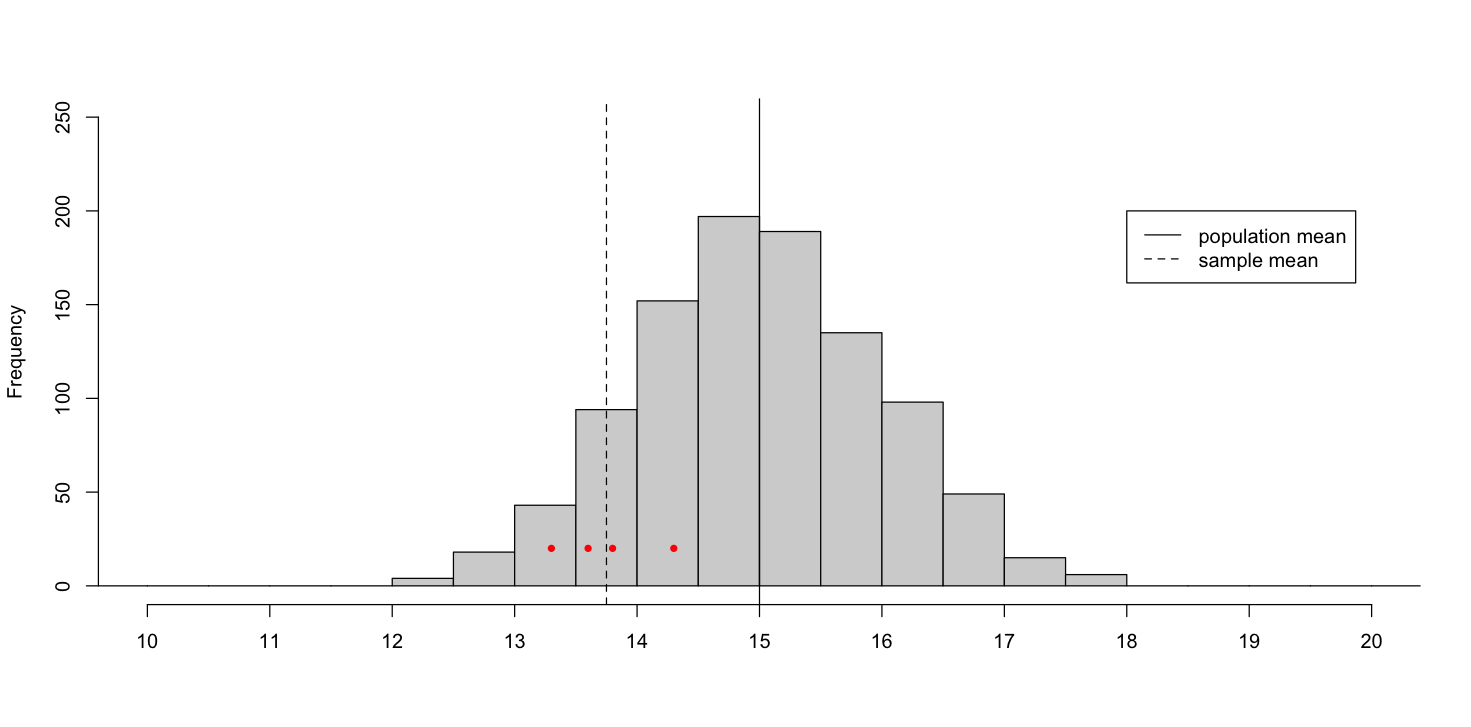
\includegraphics[width=\textwidth]{figures/02-Descriptive_statistics/degrees_of_freedom.png}
      \caption{估計母體變異數的低估問題}
      \label{fig:degrees_of_freedom}
    \end{figure}

    變異數雖然是一個很好用的分散參數,但如果仔細思考它的定義,會發現因為它是對「取值和母體平均之差值」的平方取平均,所以變異數的單位會是該變項單位的平方。例如,如果變項是收縮壓,單位是mmHg,那麼變異數的單位就會是$\text{mmHg}^2$,造成我們解釋上的困難(想像如何解釋 $100\text{mmHg}^2$!)。因此,我們再定義一個變異數的開根號為\textit{標準差} (standard deviation),作為一個新的分散參數。母體標準差通常寫作$\sigma_X$,其符號定義如下:
    \[\sigma_X = \sqrt{\frac{(\tilde{X}_1-\mu_X)^2+(\tilde{X}_2-\mu_X)^2+\cdots+(\tilde{X}_N-\mu_X)^2}{N}} = \sqrt{\frac{1}{N} \sum_{i=1}^N (\tilde{X}_i-\mu_X)^2}\]
    而估計母體標準差的樣本估計量稱為樣本標準差,通常記做$s$,其符號定義也十分直覺:
    \[s_X = \sqrt{\frac{(X_1-\bar{X})^2+(X_2-\bar{X})^2+\cdots+(X_n-\bar{X})^2}{n-1}} = \sqrt{\frac{1}{n-1} \sum_{i=1}^n (X_i-\bar{X})^2}\]
    (註:理論上上述的樣本標準差還要再進行校正才會成為母體標準差的最佳估計方法,但實務上差異不大且太過複雜,所以大多使用上述的簡單公式。)

    標準差的單位和原變項相同,因此可以看成是分布「寬度」的一個指標。若將其與平均值的組合,可以讓我們對變項做最初步的了解。在母體分布不要太奇形怪狀的情況下,我們可以套用經驗性的「68-95-99.7法則」:
    \begin{itemize}
        \item 母體約有$68\%$的取值會在 $\mu-\sigma$ 與 $\mu+\sigma$ 之間
        \item 母體約有$95\%$的取值會在 $\mu-2\sigma$ 與 $\mu+2\sigma$ 之間
        \item 母體約有$99.7\%$的取值會在 $\mu-3\sigma$ 與 $\mu+3\sigma$ 之間
    \end{itemize}
    因此,如果資料中出現離平均值兩倍標準差、甚至三倍標準差以外的觀察值,就可以進一步調查該觀察值,是否有測量錯誤的問題。
    
    如同之前在平均值的討論,我們也可以探討變項如果做線性的放大平移,會對變異數和標準差造成什麼影響。首先,直覺上,因為平移變項的數值並不會改變其分散程度,所以平移不應該改變變異數及標準差。我們可以簡單地驗證:假設我們對變項 $X$ 做平移得到 $X^* = X+b$,則我們已知母體平均數會變成 $\mu_X^* = \mu_X+b$,所以新的母體變異數為:
    \begin{align*}
        \sigma^{2*}_X &= \frac{[(\tilde{X}_1+b)-(\mu_X+b)]^2+[(\tilde{X}_2+b)-(\mu_X+b)]^2+\cdots+[(\tilde{X}_N+b)-(\mu_X+b)]^2}{N} \\
        &= \frac{[\tilde{X}_1-\mu_X]^2+[\tilde{X}_2-\mu_X]^2+\cdots+[\tilde{X}_N-\mu_X]^2}{N} = \sigma_X^2
    \end{align*}
    同樣地,樣本變異數也不會受到平移的影響。由於標準差為變異數開根號,所以也不會受到平移的影響。

    假設我們並非對變項 $X$ 做平移,而是縮放而得到 $X^* = aX$,例如把 $X$ 的測量單位從公尺變成公分,使得數值變為 100 倍,則我們已知母體平均數會變成 $\mu_X^* = a\mu_X$,所以新的母體變異數為:
    \begin{align*}
        \sigma^{2*}_X &= \frac{(a\tilde{X}_1-a\mu_X)^2+(a\tilde{X}_2-a\mu_X)^2+\cdots+(a\tilde{X}_N-a\mu_X)^2}{N} \\
        &= a^2\frac{(\tilde{X}_1-\mu_X)^2+(\tilde{X}_2-\mu_X)^2+\cdots+(\tilde{X}_N-\mu_X)^2}{N} = a^2\sigma_X^2
    \end{align*}
    因此,縮放後,母體變異數會以平方的倍數被縮放。同樣地,樣本變異數也會被平方的倍數縮放。由於標準差為變異數開根號,所以標準差的縮放倍數會和變項的縮放倍數大小相同(需加上絕對值),也就是$\sigma^*_X = |a|\sigma_X$。

    除了變異數和標準差外,\textit{全距} (range) 和 \textit{四分位差} (interquartile range, IQR) (尤其是四分位差)也會被拿來作為量化變數分散程度的描述統計量。全距的定義十分直觀,即為最大觀察值和最小觀察值之差,不過也因此全距非常容易受到極端值的影響,對於分散程度的量化效果不如其他統計量。四分位差則牽涉到百分位數的計算。我們之前計算過的中位數其實就是第 $50$ 百分位數,而第 $p$ 百分位數的計算方式為($\lceil.\rceil$為取比括號內大的最小整數)
    \[\left\{\begin{array}{lr}
        X_{(\lceil np/100 \rceil)}, & np/100 \text{非整數}\\
        \frac{1}{2}\Big[X_{(np/100)}+X_{(np/100+1)}\Big], & np/100 \text{為整數}
    \end{array}\right.\]
    第一、第二、第三四分位分別為變項的第 25、50、75 百分位數,而四分位差的定義則為第三四分位與第一四分位的差。由此可以看到,四分位差不會受到數值最大和最小 25$\%$ 資料的影響,對於極端值較不敏感。因此在實務上,如果資料分布有較多的極端值,如圖\ref{fig:descriptive_cont}中的C和D,可以考慮以四分位差取代標準差作為分散程度的指標。

    \bigskip

    \begin{custom}{思考}
        如果對資料作線性的放大平移,那麼中位數、全距和四分位差應該會如何變動?
    \end{custom}

\subsection{數值變項的描述性統計圖表}
    除了前面提到的直方圖外,另一種常用來描述連續變項分布的圖表是\textit{盒形圖} (boxplot) 或\textit{盒鬚圖} (box-and-whisker plot),如圖\ref{fig:boxplot_stem}的左圖。盒鬚圖的好處是可以在有限的空間中描繪資料的中心、分散度、偏度以及可能的\textit{離群值} (outlier)。盒鬚圖分成三部分:盒子、鬍鬚和代表離群值的圓點。盒子的部分代表變項取值的主要範圍,上下分別為變項的第三四分位 (Q3) 和第一四分位 (Q1),而中間的線段代表中位數 (M)。圓點的部分代表離群值,常見的離群值定義以四分位差 (IQR) 作為分散程度的標準:取值若落在 Q3 + 1.5 IQR 以及 Q1 - 1.5 IQR 以外,則標記為離群值。最後鬍鬚的部分則畫出非離群值之取值範圍,因此上限(U)為不大於 Q3 + 1.5 IQR 的最大觀察值,而下限(L)為不小於 Q1 - 1.5 IQR 的最小觀察值。盒鬚圖中間的小菱形並非必要,若有畫上則通常代表平均值。

    在直方圖中,每個直條僅能說明在該區間中有多少觀察值,但觀察值在區間內的分布則無從得知。當資料量比較少時,\textit{莖葉圖} (stem-and-leaf plot)可以提供比直方圖更多的資訊。在莖葉圖中,所有的觀察值都被拆成兩部分:左邊帶頭的一串數字(莖)以及最右邊的一位數字(葉)。例如 4, 10, 81 被分為 (0,4), (1,0), (8,1)。而後先把最小的莖安置在左上角,並依序向下加一至最大的莖。而後將每個觀察值的葉,按照其莖的位置,排序填入莖的右側,即可得到如圖\ref{fig:boxplot_stem}之右圖的莖葉圖。可以看到,莖葉圖保有直方圖的特性:每一個莖右邊的葉子長度即為該代表區間的觀察值數,例如落在 [40,50) 的觀察值僅有兩個。另外,在每個莖中,可以依據右邊葉子數字的分布,了解區間內資料的分布狀況。例如在 [10, 20) 這個區間中,葉的數值大多集中在小數字,也就是在這個區間中分布是比較右偏的。

    \begin{figure}[htbp]
        \centering
        \begin{minipage}{.5\textwidth}
            \centering
            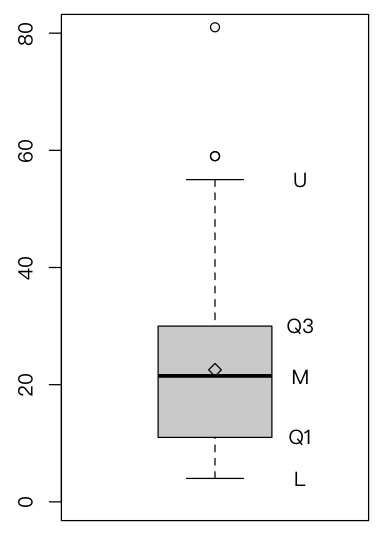
\includegraphics[width=0.9\textwidth]{figures/02-Descriptive_statistics/boxplot.png}
        \end{minipage}%
        \begin{minipage}{.5\textwidth}
            \centering
            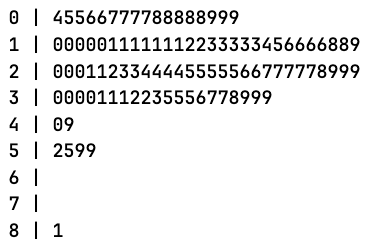
\includegraphics[width=0.9\textwidth]{figures/02-Descriptive_statistics/stem_and_leaf.png}
        \end{minipage}
        \caption{盒鬚圖與莖葉圖}
        \label{fig:boxplot_stem}
    \end{figure}

    \bigskip

    \begin{custom}{思考}
        直方圖和盒鬚圖各自提供了哪些對方所沒有的資訊?是否有可能將兩者合併?
    \end{custom}

    \begin{docexam}{(104-1醫學(一))}
        下列那個測量值較不易受到資料極端值的影響?
        
        (A) 平均值  (B) 中位數  (C) 全距  (D) 標準差
    \end{docexam}

    \begin{docexam}{(102-1醫學(一))}
        下列何種統計指標較不受極端值的影響?
        
        (A) 平均值  (B) 第75百分位數  (C) 樣本標準差  (D) 樣本標準誤
    \end{docexam}

    \begin{docexam}{(102-1醫學(一))}
        下列資料是 6 隻長有癌細胞老鼠,經過放射線治療後的存活時間(月):1.4, 1.7, 2.3, 2.5, 3.2, 3.8。如果 3.8 這筆資料在紀錄時,被錯誤地記為 38,下列哪一個敘述隊統計量的影響是正確的?
        
        (A) 中位數增加  (B) 眾數增加  (C) 平均值增加  (D) 中位數和平均值同時增加
    \end{docexam}

    \begin{docexam}{(101-1醫學(一))}
        下列資料代表 6 個接受髖關節置換手術病人的住院天數(天):4, 3, 3, 5, 4, 20,哪一個集中趨勢統計量最適合描述此資料?
        
        (A) 平均值  (B) 全距  (C) 眾數  (D) 中位數
    \end{docexam}

    \begin{docexam}{(100-2醫學(一))}
        有一位研究者想瞭解抽菸和肥胖間的相關,肥胖程度用身體質量指數測量,身體質量指數(BMI)=體重(公斤)/身高$^2$(公尺),此研究者想描述抽菸者和非抽菸者的BMI集中趨勢,下列何者統計量最適合?
        
        (A) 平均值  (B) 全距  (C) 百分比  (D) 眾數
    \end{docexam}

    \begin{docexam}{(109-1醫學(二))}
        有關描述變項的性質,下列敘述何者正確?
        
        (A) 標準誤 (standard error) 適合描述常態連續資料的分散情況
        
        (B) 幾何平均值 (geometric mean) 適合描述類別資料的集中趨勢
        
        (C) 標準差 (standard deviation) 適合描述類別資料的集中趨勢
        
        (D) 第 50 百分位數 (the 50th percentile) 適合描述連續資料的集中趨勢
    \end{docexam}

    \begin{docexam}{(108-1醫學(二))}
        關於測量尺度(measurement scale)的敘述,下列何者正確?
        
        (A) 血型為序位尺度 (ordinal scale)
        
        (B) 膽固醇值 (mg/100ml) 為等比尺度 (ratio scale) 
        
        (C) 體溫 (攝氏度 C) 為等比尺度 (ratio scale)
        
        (D) 癌症分期為等距尺度 (interval scale)
    \end{docexam}
\chapter{機率與機率分布}
    利用敘述性統計了解資料的分布後,我們就準備要步入推論性統計的範疇了。推論性統計的內涵是將資料抽樣的不確定性以系統性的方式納入考量後,給出資料隱含的結論,因此在進入推論性統計之前,我們必須先熟悉量化抽樣不確定性的數學工具-機率。在這一章,我們會先複習機率以及條件機率的定義,並說明由條件機率衍生出的貝氏定理與其實際應用。然後,我們會介紹隨機變數的概念、常見的隨機變數分布、以及這些分布的特性。本章會開始出現較多的數學符號,但大部分都只牽涉加減乘除,只有一小部分會需要用到積分符號。
    
    \begin{introduction}[第 \thechapter 章學習目標]
        \item 了解機率以及條件機率的意義
        \item 了解貝氏定理以及其於流行病學上的應用
        \item 常見的離散型與連續型分布以及其特性
    \end{introduction}

\section{基礎機率}
\subsection{機率的定義}
    \textit{機率}(probability)又稱或然率或是概率,用來度量一個事件發生可能性,定義為介於 0 和 1 之間的實數。機率越接近 1,代表事件發生的可能性越高,而機率等於 1 代表事件必然發生;反之,機率越接近 0,代表事件發生的可能性越低,而機率等於 0 代表事件不可能發生。對於機率的解釋,一般可以分成兩大流派:\textit{客觀機率}(objective probability)和\textit{主觀機率}(subjective probability)。其中客觀機率又可以分成兩種定義方式:\textit{古典機率} (classical probability) 和\textit{頻率機率} (frequentist probability)。我們可以用「擲兩個骰子得到之總點數為 3 的機率」來說明這三種機率定義方式:
    \begin{itemize}
        \item \textbf{古典機率}:古典機率是最原始的機率定義方法,此定義可以追溯到18世紀的數學家拉普拉斯(Pierre-Simon Laplace)。古典機率認為,首先要找到一群發生可能性均相同的簡單事件(simple events),例如有 $n$ 個這樣的簡單事件。然後,我們可以將我們有興趣的事件分解為 $k$ 個簡單事件的組合。這樣一來,我們有興趣的事件的發生機率就是 $k/n$。例如,擲兩個骰子後,將第一個骰子的點數 a 和第二個骰子的點數 b 記為 (a,b),就可以建構出 36 種可能性相同的簡單事件:(1,1), (1,2), (1,3), ... (1,6), (2,1), (2,2), ..., (6,6)。而我們有興趣的事件「得到總點數為 3」可以分解為兩種簡單事件 (1,2) 和 (2,1),所以「擲兩個骰子得到之總點數為 3 的機率」等於 $2/36 = 1/18$。這種定義雖然簡單直觀,但有兩個主要缺點:首先,「可能性均相同的簡單事件」含有「可能性」在裡面,所以這種定義方法有自己指涉自己的套套邏輯之嫌;另外,符合定義的簡單事件不見得存在,例如在上述的例子中,如果骰子是灌鉛的骰子,那麼就找不到可能性相同的簡單事件了。
        \item \textbf{頻率機率}:頻率機率認為,要探討事件的機率,首先必須要有可重複的隨機試驗,例如我們這裡的隨機試驗就是丟兩顆骰子並記錄點數。該隨機試驗的所有可能結果所組成的集合叫做\textit{樣本空間}(sample space),通常記為$\Omega$,因此例子中的樣本空間就是 36 種可能點數組合的集合,也就是 $\Omega = \{(1,1), (1,2), (1,3), ... (1,6), (2,1), (2,2), ..., (6,6)\}$。注意到這裡我們並未要求樣本空間中所有結果的可能性相等,因此和古典機率不同。\textit{事件}(event)就是樣本空間的子集合,例子中「得到總點數為 3」的事件即對應到 $A = \{(1,2),(2,1)\}$ 這個子集合。重複該試驗多次以後,事件發生的次數 $k$ 和試驗次數 $n$ 的比值雖可能不固定,但是隨著試驗次數增多終將會趨近一個數值,而該數值就是事件發生的機率。頻率機率的定義解決了古典機率的兩大缺點,但其奠基於「可重複隨機試驗」的事實也引起批評:如果我們關心的事件不可能重複試驗,例如「明天台北發生地震」、「某國總統被成功彈劾」或「某病患將在 24 小時內離開加護病房」,那麼頻率機率的定義就顯得不合適。
        \item \textbf{主觀機率}:主觀機率認為機率是個人信念的一種度量,因此「擲兩個骰子得到之總點數為 3 的機率」是我們基於已知的事實(例如骰子的製作過程、投擲的隨機性)評估出擲出骰子後總點數為 3 的可能性。和頻率機率的差異在於,頻率機率認為存在可重複的隨機試驗,該試驗的條件可能未知,但已固定。主觀機率則認爲針對試驗的方方面面的不確定性和主觀認知,都應該納入機率考量。因此不同人針對同一事件的主觀機率,也會隨著每個人的信念和經驗而不同。
    \end{itemize}
    在後續的課程中,大部分時候我們選擇的機率定義為頻率機率,但必要的時候,我們也會改用主觀機率以方便實務上的解釋。讀者閱讀時也不妨想想各處提到的機率是用哪種方式定義比較合適。
\subsection{機率的基本性質}
    在頻率機率的定義下,假設樣本空間是 $\Omega$,而 $A$, $B$ 代表任意的事件,我們定義如下:
    \begin{itemize}
        \item $\PP(A)$ 代表 $A$ 事件發生的機率。
        \item $\bar{A} = \Omega \backslash A$ 為 $A$ 的\textit{補事件} (complementary event),也就是 「$A$沒有發生」的事件。
        \item $A \cap B$ 為 $A$ 和 $B$ 兩個事件的交集,對應到「$A$與$B$均發生」的事件。
        \item $A \cup B$ 為 $A$ 和 $B$ 兩個事件的聯集,對應到「$A$或$B$發生」的事件。
        \item 當 $A \cap B = \phi$,即兩個事件的交集為空集合時,我們稱 $A$ 和 $B$ 兩個事件\textit{互斥} (mutually exclusive)。此時這兩個事件不可能同時發生,因為他們代表的結果完全沒有交集。
    \end{itemize}
    舉例來說,如果 $\Omega = \{1,2,3,4,5,6\}$ 是擲一顆骰子的點數樣本空間,$A = \{2,4,6\}$ 是擲到偶數的事件,$B = \{1,2,3\}$ 是擲到小點的事件,$C = \{5\}$ 是擲到 5 點的事件。那麼 $A$ 的補事件是 $\bar{A} = \{1,3,5\}$,也就是擲到奇數的事件。$A \cap B = \{2\}$ 是擲到偶數小點的事件。$A \cup B = \{1,2,3,4,6\}$ 是擲到偶數或小點的事件。而因為 $A \cap C = \phi$,所以 $A$ 和 $C$ 是互斥事件。

    根據上述的定義,下面幾個機率性質必須要成立:
    
    \begin{itemize}
        \item $\PP(\Omega) = 1$:樣本空間本身就是樣本空間的子集合,所以樣本空間也是一個事件(也就是觀察到所有可能結果的組合)。這個性質說明\textbf{所有可能結果的總機率應為 1} 。
        \item $0 \le \PP(A) \le 1$:這個性質說明\textbf{機率必然是0到1之間的實數}。
        \item $A \cap B = \phi \Rightarrow \PP(A \cup B) = \PP(A) + \PP(B)$:這個性質說明\textbf{兩個事件若互斥,則至少一個事件發生的機率為兩個事件的機率相加}。
    \end{itemize}

    根據這些性質,因為 $A \cap \bar{A} = \phi$,所以 $\PP(A) + \PP(\bar{A}) = \PP(A \cup \bar{A}) = \PP(\Omega) = 1$,也就是不發生 $A$ 事件的機率和發生 $A$ 事件的機率總和為 1,非常符合直覺。另外,根據簡單的集合性質我們也能證明,在 $A$ 與 $B$ 不互斥的情況下的\textit{加法原則} (addition rule):
    \[\PP(A \cup B) = \PP(A) + \PP(B) - \PP(A \cap B)\]


\subsection{條件機率與獨立事件}

    接下來我們要說明一個比較複雜的概念:\textit{條件機率} (conditional probability)。條件機率評估的是「給定某事件發生的情況下,另外一個事件發生的機率」,例如「在 COVID-19 快篩呈陽性的情況下,真的感染 COVID-19 的機率」。以數學符號來表示的話,給定 $B$ 事件下 $A$ 事件發生的條件機率記為 $\PP(A|B)$。條件機率的計算方法十分直覺:假設我們重複做實驗做了 $n$ 次,其中大約會有 $n\PP(B)$ 次發生 $B$ 事件,而約有 $n\PP(A \cap B)$ 次除了發生 $B$ 事件、還發生了 $A$ 事件。因此,給定 $B$ 事件下 $A$ 事件發生的機率就可以寫為
    \[\PP(A|B) = \frac{n\PP(A \cap B)}{n\PP(B)} = \frac{\PP(A \cap B)}{\PP(B)}\]
    舉例來說,如果我們想知道擲兩枚公正骰子,給定點數和為4的情況下,兩個骰子的點數不同的機率為多少,也就是$\PP(\text{兩個骰子點數不同}|\text{點數和為4})$。簡單計算可以得知,點數和為 4 的機率 $\PP(\text{點數和為4}) = 3/36$。點數和為 4 且兩個骰子點數不同的機率為 $\PP(\text{(兩個骰子點數不同)}\cap\text{(點數和為4)}) = 2/36$。所以
    \[\PP(\text{兩個骰子點數不同}|\text{點數和為4}) = \frac{\PP(\text{(兩個骰子點數不同)}\cap\text{(點數和為4)})}{\PP(\text{點數和為4})} = \frac{2}{3}\]

    \bigskip

    \begin{custom}{思考}
        按照條件機率的定義,如果 $\PP(B) \ne 0$,$\PP(A|B)$ 是否可能大於 1?為什麼?
    \end{custom}

    \bigskip

    如果一個事件發生與否,並不會影響到另一個事件發生的機率,那麼這兩個事件應該互不相關。從這個角度來看,兩個事件 $A$ 和 $B$ 互不相關應該意謂著 $\PP(A|B) = \PP(A)$ 而且 $\PP(B|A) = \PP(B)$。根據條件機率的定義,這兩個式子都導向同一個結果:
    \[\PP(A \cap B) = \PP(A) \PP(B)\]
    如果兩個事件 $A$ 和 $B$ 滿足上述關係,他們就被稱為\textit{獨立} (independent)事件。反之,則被稱為\textit{不獨立}或\textit{相依} (dependent)事件。在前面的例子中,兩個骰子點數不同的機率為 $30/36$,點數和為 4 的機率為 $3/36$,但骰子點數不同且點數和為 4 的機率為 $2/36$。顯然 $(30/36)(3/36) \ne 2/36$,所以「兩個骰子點數不同」和「點數和為 4」這兩個事件不獨立。
    
    \bigskip

    \begin{custom}{思考}
        互斥事件是否有可能是獨立事件?如果有可能,是在什麼情況下才會成立?
    \end{custom}

    \bigskip

    條件機率在流行病學的應用十分重要,尤其是篩檢診斷結果的判讀。臨床上有許多疾病的黃金診斷標準十分耗費資源,因此就公共衛生角度而言,較佳的策略是先進行一個準確度較低的篩檢,待篩檢陽性後再進行較昂貴耗時的診斷檢查。例如 HIV 的黃金診斷標準需經過抗體免疫層析、西方墨點法或分子生物學核酸檢測,但有疑慮的感染者則建議先採指尖血或唾液做初步篩檢,呈現陽性後再進行確認檢驗。篩檢結果的結果判讀中,有下列的重要參數需要評估(以表\ref{tab:screening_high_risk}為例):
    \begin{itemize}
        \item \textit{盛行率} (Prevalence):$\PP(\text{有疾病})$,即總體受檢者有疾病的比例。在下表中為$7000/10000 = 0.7$。
        \item \textit{敏感度} (Sensitivity):$\PP(\text{篩檢陽性}|\text{有疾病})$,即有疾病的人篩檢呈陽性的機率。在下表中為$5600/7000 = 0.8$。
        \item \textit{特異度} (Specificity):$\PP(\text{篩檢陰性}|\text{無疾病})$,即無疾病的人篩檢呈陰性的機率。在下表中為$2700/3000 = 0.9$。
        \item \textit{陽性預測率} (Positive predictive value, PPV):$\PP(\text{有疾病}|\text{篩檢陽性})$,即篩檢陽性的人有疾病的機率。在下表中為$5600/5900 \approx 0.949$。
        \item \textit{陰性預測率} (Negative predictive value, NPV):$\PP(\text{無疾病}|\text{篩檢陰性})$,即篩檢陰性的人無疾病的機率。在下表中為$2700/4100 \approx 0.659$。
    \end{itemize}

    \begin{table}[htbp]
        \begin{center}
            \begin{tabular}{c|cc|c}
                \toprule
                 & \textbf{有疾病} & \textbf{無疾病} & 總和\\
                \hline
                \textbf{篩檢陽性} & 5600 & 300 & 5900\\
                \textbf{篩檢陰性} & 1400 & 2700 & 4100\\
                \hline
                總和 & 7000 & 3000 & 10000\\
                \bottomrule
            \end{tabular}
            \caption{高風險族群篩檢結果\label{tab:screening_high_risk}}
        \end{center}
    \end{table}

    從這裡可以觀察到,$\PP(A|B)$ 和 $\PP(B|A)$ 是兩個完全不同的機率。此處篩檢陽性時罹病的機率很高,到達約 0.95,但即便篩檢工具的特異度已經高達 0.9,但是在盛行率較高的高風險族群中,篩檢陰性者的沒病機率仍僅有約 0.66。反之,如果我們使用同樣敏感度和特異度篩檢工具,但用在風險較低的族群中,結果可能會不一樣。假設同樣是 10000 人的族群,但盛行率降為 0.3,那麼罹病的人應該有 3000 人,未罹病的人則為 6000 人。罹病的 3000 人中,因篩檢工具敏感度為 0.8,所以有 2400 人會呈現篩檢陽性。未罹病的 7000 人中,因篩檢工具特異度為 0.9,所以有 6300 人會呈現篩檢陰性。我們可以把以上的數字填入表格中,如表\ref{tab:screening_low_risk}:

    \begin{table}[htbp]
        \begin{center}
            \begin{tabular}{c|cc|c}
                \toprule
                 & \textbf{有疾病} & \textbf{無疾病} & 總和\\
                \hline
                \textbf{篩檢陽性} & 2400 & 700 & 3100\\
                \textbf{篩檢陰性} & 600 & 6300 & 6900\\
                \hline
                總和 & 3000 & 7000 & 10000\\
                \bottomrule
            \end{tabular}
            \caption{低風險族群篩檢結果\label{tab:screening_low_risk}}
        \end{center}
    \end{table}

    \begin{itemize}
        \item \textit{陽性預測率}:$\PP(\text{有疾病}|\text{篩檢陽性}) = 2400/3100 \approx 0.774$。
        \item \textit{陰性預測率}:$\PP(\text{無疾病}|\text{篩檢陰性}) = 6300/6900 \approx 0.913$。
    \end{itemize}
    可以看到,盛行率下降的情況下,陰性預測率陡然攀升至 0.913,而陽性預測率則變得不如預期。因此,判讀篩檢結果時,除了篩檢工具的敏感度和特異度外,還要將盛行率納入考量。舉例來說,如果在疫情和緩而且完全無症狀的情況下進行 COVID 快篩,此時盛行率相對很低,因此即使篩檢陽性,實際上感染 COVID 的機會也很低;反之,如果疫情正在快速蔓延且症狀明確,則盛行率相對較高,當篩檢陽性時就很可能已經感染。

    \bigskip

    \begin{custom}{思考}
        雖然理想狀態下,我們希望篩檢工具同時具有高敏感度及高特異度,但實際上在篩檢工具的設計上,這兩者通常是個權衡關係。如果一個疾病的黃金標準檢驗很昂貴,但有病時並不需要太急著治療,那麼我們設計篩檢的目的應該要儘量確定陰性者沒病(提高 NPV)還是確定陽性者有病(提高 PPV),此時應該選擇提高篩檢工具的敏感度還是特異度?反之,如果一個疾病的黃金標準檢驗相對便宜,但有病時必須要馬上給予治療,此時的決策應為何?
    \end{custom}

\subsection{貝氏定理}
    在前面的例子中,我們為了算出盛行率降低後陽性預測率和陰性預測率的變化,藉由假設總族群有 10000 人,算出表格中的所有人數後,再依據定義算出陽性和陰性預測率。如果我們把這些數字都符號化,將總人數記作 $n$,將有疾病的事件寫作 $D$,篩檢陽性的事件寫作 $T$,那麼表格就會變成如表 \ref{tab:Bayes}:

    \begin{table}[htbp]
        \begin{center}
            \begin{tabular}{c|cc|c}
                \toprule
                 & $D$ & $\bar{D}$ & 總和\\
                \hline
                $T$ & $n\PP(D)\PP(T|D)$ & $n\PP(\bar{D})\PP(T|\bar{D})$ & $n[\PP(D)\PP(T|D) + \PP(\bar{D})\PP(T|\bar{D})]$\\
                $\bar{T}$ & $n\PP(D)\PP(\bar{T}|D)$  & $n\PP(\bar{D})\PP(\bar{T}|\bar{D})$ & $n[\PP(D)\PP(\bar{T}|D) + \PP(\bar{D})\PP(\bar{T}|\bar{D})]$\\
                \hline
                總和 & $n\PP(D)$ & $n\PP(\bar{D})$ & $n$\\
                \bottomrule
            \end{tabular}
            \caption{貝氏定理的說明\label{tab:Bayes}}
        \end{center}
    \end{table}
    
    由表中的數據試著計算陽性預測率,就可以得到著名的\textit{貝氏定理}(Bayes' Theorem):
    \[\PP(D|T) = \frac{\PP(T|D)\PP(D)}{\PP(T|D)\PP(D) + \PP(T|\bar{D})\PP(\bar{D})}\]
    貝氏定理最早是由英國的牧師兼數學家貝葉斯(Thomas Bayes, 1701-1761)提出,並由他的友人替他整理發表。在該定理中,我們可以把分子的 $\PP(D)$ 移下來,把定理寫成
    \[\PP(D|T) = \Bigg(\frac{\PP(T|D)}{\PP(T|D)\PP(D) + \PP(T|\bar{D})\PP(\bar{D})}\Bigg) \PP(D)\]
    在我們做篩檢前,對於族群的每個人的罹病機率只能用總體的盛行率 $\PP(D)$ 估計,因此 $\PP(D)$ 也被稱為患病的\textit{先驗機率} (prior probability)。做篩檢後得知病患篩檢陽性後,我們對該病患的罹病機率估計變成了 $\PP(D|T)$,因此 $\PP(D|T)$ 也被稱為得知篩檢陽性後患病的\textit{後驗機率} (posterior probability)。而中間大括弧的部分就是將先驗機率\textit{更新}(update)為後驗機率的因子,也可看作篩檢陽性帶給我們的資訊(不過此處的因子和疾病的先驗機率仍然有關)。例如在表\ref{tab:screening_high_risk}中,各病患的患病先驗機率是 0.7,一旦篩檢呈現陽性,患病的後驗機率就被更新到 0.949。綜上所述,我們可以寫作如下:
    \[\text{後驗機率}=\text{篩檢陽性的更新因子}\times\text{先驗機率}\]
    進一步來說,如果我們寫出貝氏定理針對未患病機率的公式(把 $D$ 換成 $\bar{D}$),可以得到:
    \[\PP(\bar{D}|T) = \Bigg(\frac{\PP(T|\bar{D})}{\PP(T|\bar{D})\PP(\bar{D}) + \PP(T|D)\PP(D)}\Bigg) \PP(\bar{D})\]
    將這個式子與前面的式子相除後,即得:
    \[\frac{\PP(D|T)}{\PP(\bar{D}|T)} = \frac{\PP(T|D)}{\PP(T|\bar{D})} \times \frac{\PP(D)}{\PP(\bar{D})}\]
    等式右邊第二項 $\frac{\PP(D)}{\PP(\bar{D})}$ 是先驗的患病機率除以未患病機率。一般我們把「發生機率除以未發生機率」的形式稱做\textit{勝算}(odds),例如一枚公正銅板出現正面的勝算為 1,一顆公正骰子擲出一點的勝算為 1/5。因此,$\frac{\PP(D)}{\PP(\bar{D})}$ 是先驗的患病勝算。同理,等號左邊的 $\frac{\PP(D|T)}{\PP(\bar{D}|T)}$ 則是後驗的得病勝算。中間的 $\frac{\PP(T|D)}{\PP(T|\bar{D})}$中,分子是「患病者篩檢陽性的機率(敏感度)」,分母則是「未患病者篩檢陽性的機率(一減特異度)」,所以整個分數代表「患病者相對於未患病者的篩檢陽性機率比值」。這個分數僅和篩檢工具的敏感度和特異度有關,可視為篩檢工具特有的診斷力特徵,被稱為\textit{陽性概似比} (positive likelihood ratio, LR+)。綜上所述,在篩檢陽性的時候我們有:
    \[\text{後驗罹病勝算}=\text{陽性概似比(LR+)}\times\text{先驗罹病勝算}\]
    同理,在篩檢陰性的時候我們有
    \[\frac{\PP(D|\bar{T})}{\PP(\bar{D}|\bar{T})} = \frac{\PP(\bar{T}|D)}{\PP(\bar{T}|\bar{D})} \times \frac{\PP(D)}{\PP(\bar{D})}\]
    此處我們稱$\frac{\PP(\bar{T}|D)}{\PP(\bar{T}|\bar{D})}$,也就是「一減敏感度」除以「特異度」為陰性概似比(negative likelihood ratio, LR-),因此在篩檢陰性的時候我們可寫作
    \[\text{後驗罹病勝算}=\text{陰性概似比(LR-)}\times\text{先驗罹病勝算}\]
    由此可見,只要知道篩檢工具的陽性及陰性概似比,就可以根據病患的先驗罹病勝算及檢驗結果推斷出其後驗罹病勝算。因此實證醫學中,這兩個數值是評估篩檢或診斷工具有效度的重要指標。

    \bigskip
    
    \begin{custom}{思考}
        在日劇欺詐遊戲中,福永和女主角神崎對賭。福永拿出兩張撲克牌放入袋中,一張是正常牌,一張則是兩面都是牌背的錯誤牌。福永和神崎輪流隨機從袋中取出一張撲克牌,若取出時亮出牌面則放回重抽,取出時為牌背則翻開撲克牌確認。若該牌為正常牌則神崎贏,若該牌為錯誤牌則福永贏。福永誆騙神崎說這是一個 50\%-50\% 的公平遊戲,但實際上神崎每一把贏的機率為何?
    \end{custom}

\section{離散型機率分布}

    了解機率的意義後,我們就可以用機率的語言去描述一個隨機實驗會出現的結果。首先,為了數學上處理方便,若實驗的結果並非數值,我們會先將可能的結果編碼。例如丟一個銅板時,我們可以把正面的結果編碼為 $1$,反面的結果編碼為 $0$。此時隨機試驗就像是一台機器,上面有一個按鈕。按下按鈕後,隨機試驗就會吐出一個結果數值。這個未知的結果我們稱之為\textit{隨機變數} (random variable),通常用大寫的英文字母表示。以前面的銅板為例,我們可以把丟銅板的結果用隨機變數 $X$ 表示,而 $X$ 的取值可能是 $0$ 或 $1$。
    
    隨機變數各種取值的可能性被稱為其機率分布 (probability distribution),或簡稱為分布。描述 $X$ 的分布時,我們可以把兩種取值出現的機率做一個表列,例如 $\PP(X = 1) = 0.8;\; \PP(X = 0) = 0.2$。為了更加簡化,我們定義 $X$ 的機率質量函數 (probability mass function, 常用小寫 $f$ 表示)為:
    \[f_X(x) := \PP(X = x)\]
    如此一來, $X$ 的機率質量函數取值如下
    \[f_X(x) = \left\{\begin{array}{rl}
            0.8, & x = 1\\
            0.2, & x = 0\\
            0, & \text{其他}
        \end{array}\right.\]
    有了這個函數就可以完整描述 $X$ 的分布。注意到由於總機率等於 1,所以機率質量函數裡面的各取值對應的機率總和必然等於 1 (0.8+0.2=1)。如果另一個隨機變數 $Y$ 的可能取值是所有的非負整數 $0, 1, 2, ...$,那麼只要知道 $f_Y(0), f_Y(1), f_Y(2), ...$ 的數值,就可以完整描述 $Y$ 的分布。因此,機率質量函數就像隨機變數的指紋一樣,可以\textbf{完全}定義隨機變數的分布。注意到要能夠寫出機率質量函數的話,隨機變數的可能取值必須要是可數的 (countable)。這類機率分布被稱為\textit{離散型機率分布} (discrete probability distribution)。
    
    除了機率質量函數以外,另一個常用的函數是\textit{累積分配函數} (cumulative distribution function, 常用大寫 $F$ 來表示),其定義為:
    \[F_X(x) := \PP(X \le x)\]
    例如上述銅板的例子中,我們就有
    \[F_X(x) = \left\{\begin{array}{rl}
        0, & x < 0\\
        0.2, & x < 1\\
        1, & x \ge 1
    \end{array}\right.\]
    
    為了對隨機變數做進一步瞭解,我們可以把隨機變數的機率分布看作是一個母體,而隨機變數的取值就是從母體抽樣的結果。因此,如果我們知道機率分布的敘述性參數,例如作為位置參數的平均值、和作為分散參數的變異數和標準差,那麼就知道相對應隨機變數的取值中心以及分散程度。隨機變數機率分布的平均值也被稱作隨機變數的\textit{期望值} (expected value),其計算方法如下(其中 $\mathcal{X}$ 是 隨機變數 $X$ 所有可能取值的集合,也被稱為 $X$ 的\textit{支撐集} (support))。
    \[\EE(X) = \sum_{x\in\mathcal{X}} x \cdot f_X(x)\]
    可以看到期望值的計算方法,是把每個可能的取值依出現機率做\textbf{加權平均}。例如前面擲銅板的例子中,$X$ 的期望值就是 $\EE(X) = 1 \times 0.8 + 0 \times 0.2 = 0.8$。同理,隨機變數機率分布的變異數和標準差計算方法為
    \begin{align*}
        var(X) &= \sum_{x\in\mathcal{X}} (x-\EE(X))^2 \cdot f_X(x)\\
        sd(X) &= \sqrt{var(X)}
    \end{align*}
    這裡 $var(X)$ 的算法也是加權平均,但是要平均的是取值和期望值的距離平方,符合我們在敘述性統計時的作法。不過,上述的計算過程通常比較繁瑣,所以我們會使用另外一個計算公式(注意到 $\EE(X)$ 是一個數字,和加總符號使用的 $x$ 無關,所以在很多地方可以提出加總符號外):
    \begin{align*}
        var(X) &= \sum_{x\in\mathcal{X}} (x-\EE(X))^2 \cdot f_X(x)\\
        &= \sum_{x\in\mathcal{X}} [x^2 - 2x\EE(X) + (\EE(X))^2] \cdot f_X(x)\\
        &= \Big[\sum_{x\in\mathcal{X}} x^2 \cdot f_X(x)\Big] - \Big[\sum_{x\in\mathcal{X}} 2x\EE(X) \cdot f_X(x)\Big] + \Big[\sum_{x\in\mathcal{X}} (\EE(X))^2 \cdot f_X(x)\Big]\\
        &= \Big[\sum_{x\in\mathcal{X}} x^2 \cdot f_X(x)\Big] - 2\EE(X)\Big[\sum_{x\in\mathcal{X}} x \cdot f_X(x)\Big] + (\EE(X))^2\Big[\sum_{x\in\mathcal{X}} f_X(x)\Big]\\
        &= \Big[\sum_{x\in\mathcal{X}} x^2 \cdot f_X(x)\Big] - 2\EE(X)\EE(X) + (\EE(X))^2\\
        &= \EE(X^2) - (\EE(X))^2
    \end{align*}
    倒數第二行的第一項是把每個可能取值的平方做加權平均,因此在符號上寫作 $\EE(X^2)$,也就是 $X^2$ 的期望值。前面擲銅板的例子中,$X^2$ 的期望值是 $\EE(X^2)=1^2 \times 0.8 + 0^2 \times 0.2 = 0.8$,所以 $X$ 的變異數為 $\EE(X^2) - (\EE(X))^2 = 0.8-0.8^2 = 0.16$,而 $X$ 的標準差則為 $\sqrt{0.16} = 0.4$。

    當我們對隨機變數作線性轉換的時候,它的期望值和變異數的變化就如同我們在敘述性統計所提到的:
    \begin{align*}
        \EE(aX+b) &= a\EE(X) + b\\
        var(aX+b) &= a^2 var(X)
    \end{align*}
    而當我們對兩個隨機變數 $X, Y$ 做相加減時,期望值也會相加減
    \[\EE(X \pm Y) = \EE(X) \pm \EE(Y)\]
    如果這兩個隨機變數還互相\textbf{獨立},那麼變異數則會相加
    \[var(X \pm Y) = var(X) + var(Y)\]
    
    以下我們介紹幾個生物醫學統計中常用到的離散分布以及其性質:

\subsection{白努利分布}

    前面我們提到擲銅板的例子中,我們根據 $X=0$ 和 $X=1$ 的機率寫出隨機變數 $X$ 的機率質量函數。一般性地來說,如果隨機變數 $X$ 僅能取值 $0$ 或 $1$,而且把 $X=1$ 的機率寫為 $p$,那麼由於機率總和為 1,$X=0$ 的機率就必然是 $1-p$。根據這樣的設定所得的機率質量函數為
    \[f_X(x) = \left\{\begin{array}{rl}
        p, & x = 1\\
        1-p, & x = 0
    \end{array}\right.\]
    這個機率質量函數作圖如圖\ref{fig:bernoulli},其所對應的分布被稱為\textit{白努利分布} (Bernoulli distribution)。白努利分佈有一個參數 $p$,代表隨機變數取值為 $1$ 的機率。的當一個隨機變數 $X$ 服從參數為 $p$ 的白努利分布,我們會寫作
    \[X \sim Bernoulli(p)\]

    \begin{figure}[htbp]
      \centering
      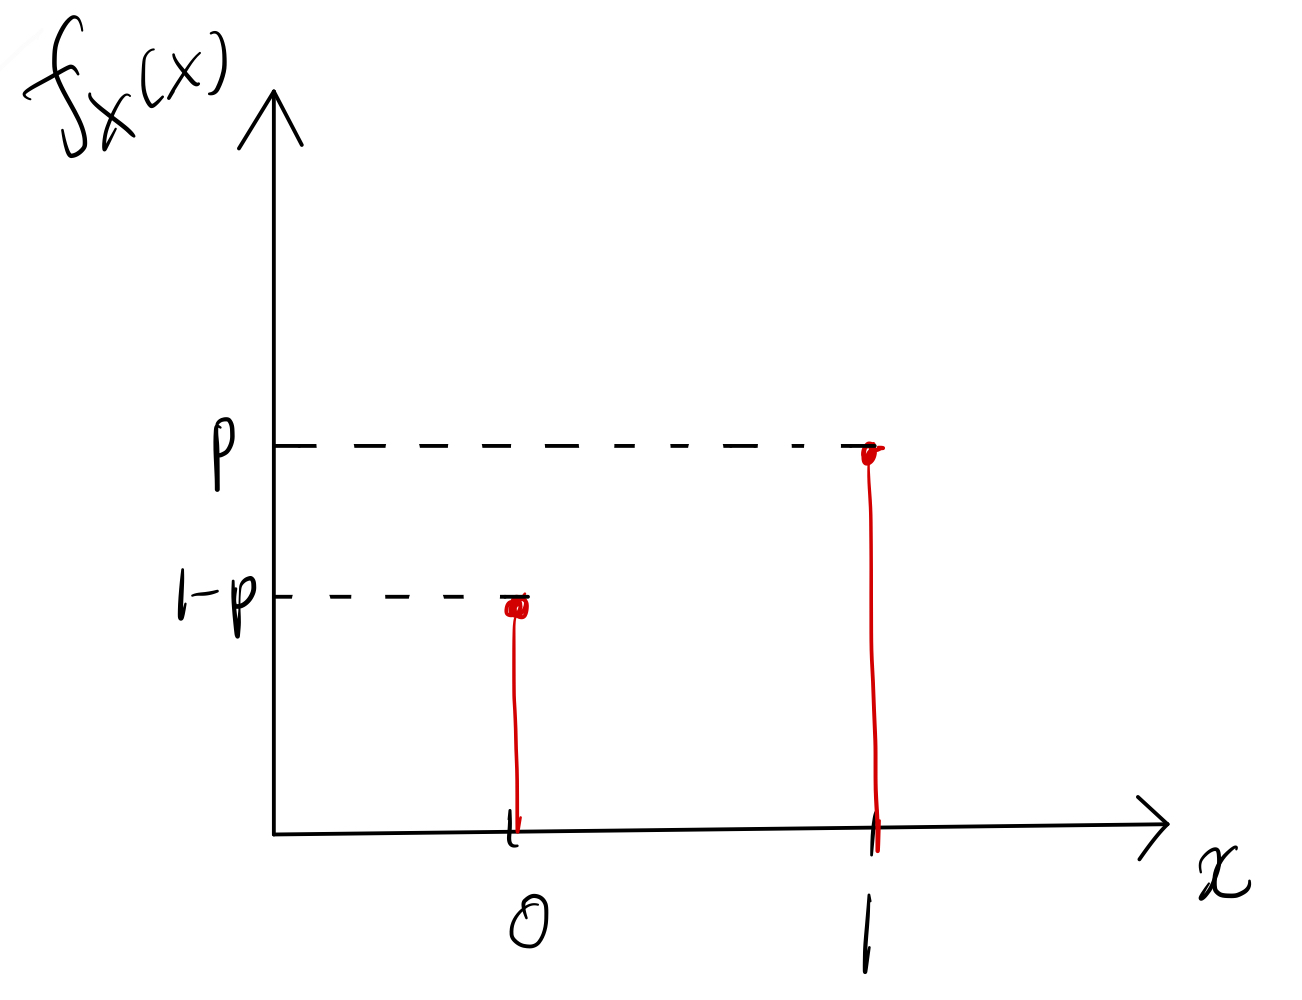
\includegraphics[width=0.5\textwidth]{figures/03-Probability_distribution/Bernoulli.jpeg}
      \caption{白努利分佈的機率質量函數}
      \label{fig:bernoulli}
    \end{figure}
    
    白努利分布的命名來自於瑞士數學家 Jacob Bernoulli(1654-1705),是最簡單也最常用的的離散型機率分布。所有的二元變數,舉凡性別的男女、疾病發病與否、是否接受治療、收縮壓是否於140毫米汞柱以上,將有興趣的類別編碼為 1,另一個類別編碼為 0 後,其分布均可用白努利分布來描述,其中參數 $p$ 為類別為 $1$ 的機率。簡單計算白努利分布之期望值和變異數可得到期望值為 $p$,變異數為 $p(1-p)$。

    \begin{custom}{思考}
        我們知道變異數是分佈取值分散性的度量。根據這個想法,白努利分布的變異數應該在 $p$ 取值多少時為最小、$p$ 取值多少時為最大?剛剛我們算出分布的變異數為 $p(1-p)$,這個結果是否符合你的預測?
    \end{custom}

\subsection{二項式分布}
    我們剛剛提到的白努利分布對應到的是擲一次銅板並觀察是否為正面。如果我們擲了同一枚銅板多次,然後再計算正面的次數,對應到的就是\textit{二項式分佈} (binomial distribution)。假設我們擲了 3 次銅板,每次擲銅板時正面機會均為 0.8,那麼有 2 次正面的情況共有 3 種:第一、二次正面、第三次反面;第一、三次正面、第二次反面;第二、三次正面、第一次反面。情況的總數可以用高中的組合數來計算,也就是$C^3_2$或寫做$\binom{3}{2}$。每種情況都是兩次正面、一次反面,所以機率都是 $0.8^2 \cdot 0.2$。因此,總共出現 2 次正面的機率可以寫作 $\binom{3}{2} 0.8^2 \cdot 0.2 = 0.384$。按照上述的算法,如果我們把 $X$ 令為投擲 $n$ 次銅板,每次正面機會為 $p$ 時,出現正面次數的隨機變數,那麼 $X$ 的機率質量函數可寫為:
    \[f_X(x) = \binom{n}{x} p^x (1-p)^{n-x},\qquad x \in \{0,1,2,...,n\}\]
    此時我們稱隨機變數 $X$ 服從次數參數為 $n$,機率參數為 $p$ 的二項式分布,寫作
    \[X \sim Binomial(n,p)\]

    二項式分佈的偏度隨著機參數率 $p$ 的不同而可能為左偏、對稱或右偏。如圖\ref{fig:binomial}繪製的機率質量函數所示,當 $p<0.5$ 時,二項式分佈呈現右偏;當 $p>0.5$ 時,二項式分佈呈現左偏;當 $p=0.5$ 時,二項式分佈為左右對稱。
    \begin{figure}[htbp]
      \centering
      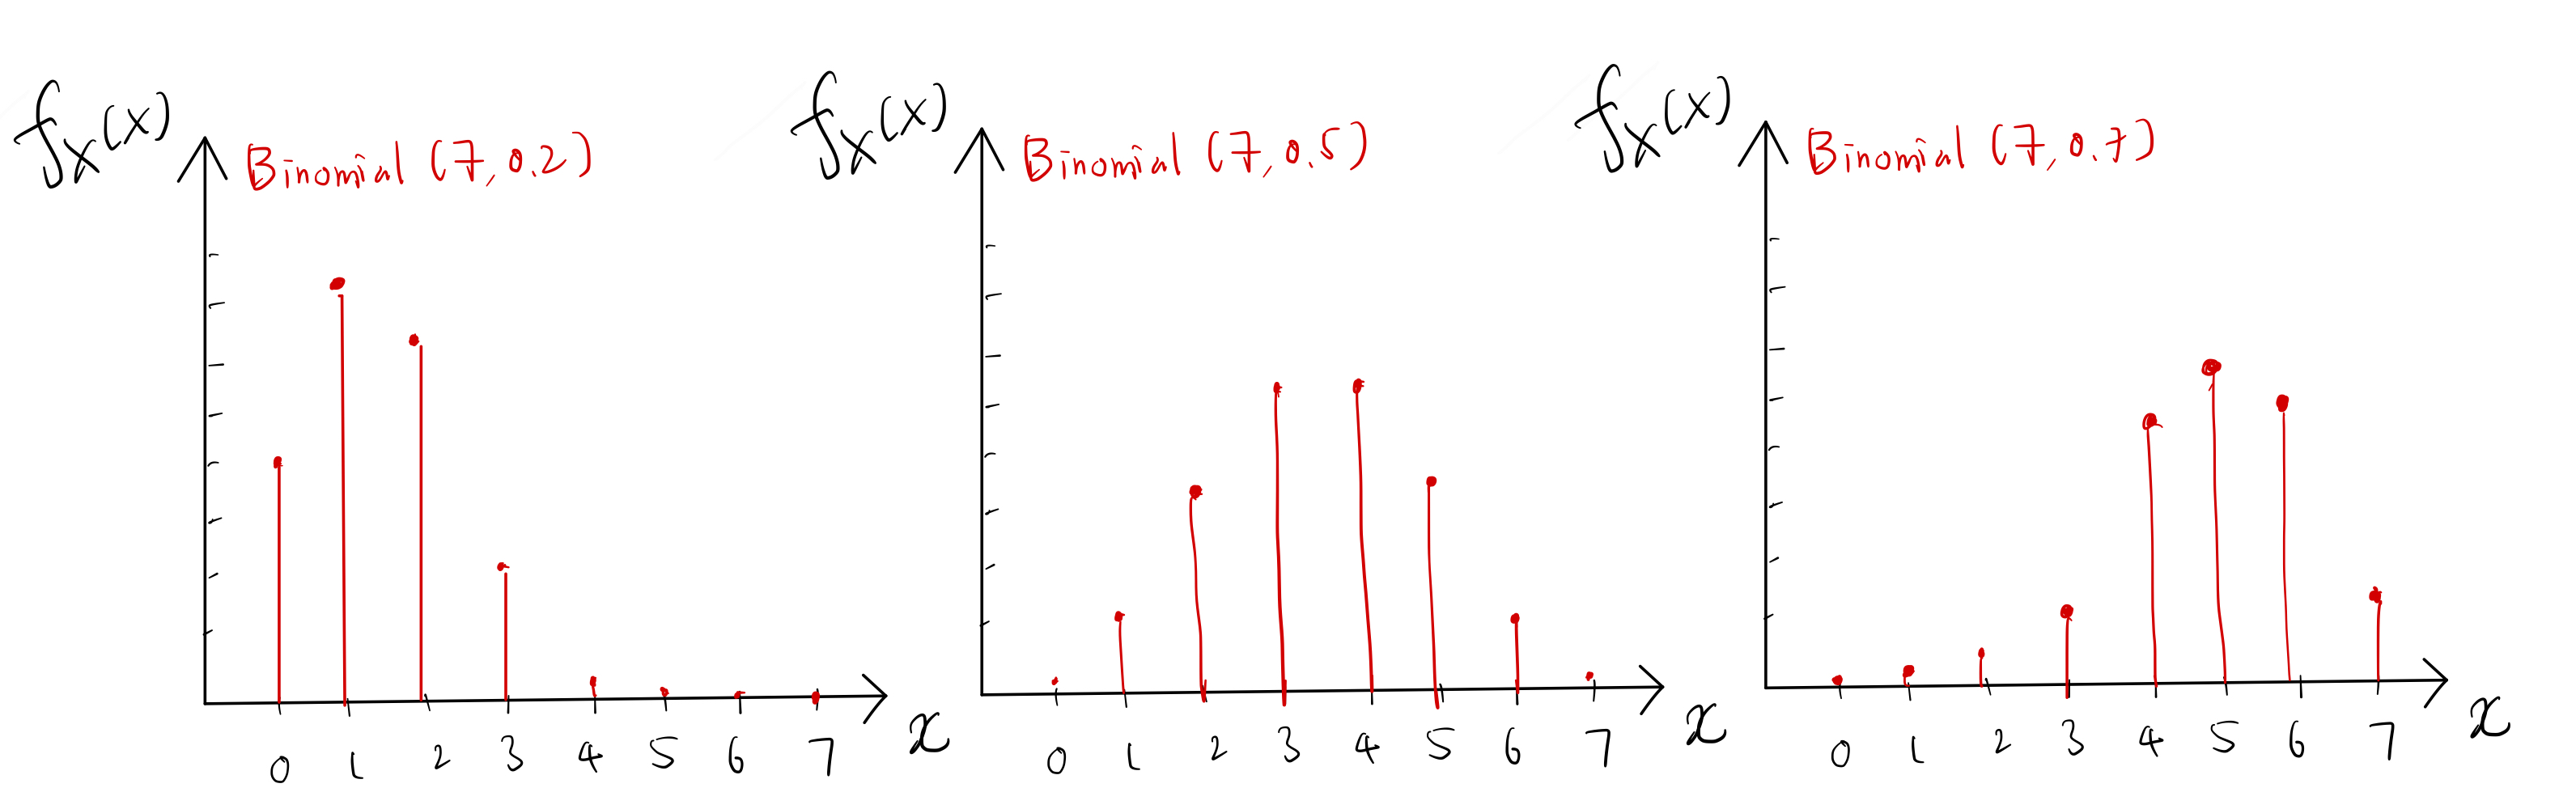
\includegraphics[width=\textwidth]{figures/03-Probability_distribution/Binomial.jpeg}
      \caption{二項分佈的機率質量函數}
      \label{fig:binomial}
    \end{figure}
    二項式分佈的期望值和變異數如果要從機率質量函數去推導,會需要相當麻煩的代數計算。但我們可以想像,二項式分佈所代表的銅板正面總次數,可以視為每次擲銅板時的正面次數(非 1 即 0)相加。如果 $X_1, X_2, ..., X_n$ 代表每次擲銅板正面與否,那麼他們都應該服從機率參數為 $p$ 的白努利分佈,而我們最終關心的正面總次數 $X = X_1 + X_2 + ... + X_n$。由於每次擲銅板的結果都是獨立的,所以根據我們前面提到有關期望值和變異數的性質:
    \begin{align*}
        \EE(X) &= \EE(X_1 + X_2 + ... + X_n)&\\
        &= \EE(X_1) + \EE(X_2) + ... + \EE(X_n) &\text{(相加的期望值等於期望值相加)}\\
        &= p + p + ... + p&\text{(每次擲銅板都服從} Bernoulli(p)\text{)}\\
        &= np&\\
        var(X) &= var(X_1 + X_2 + ... + X_n)&\\
        &= var(X_1) + var(X_2) + ... + var(X_n) &\text{(獨立隨機變數相加的變異數等於變異數相加}\\
        &= p(1-p) + p(1-p) + ... + p(1-p)&\text{(每次擲銅板都服從} Bernoulli(p)\text{)}\\
        &= np(1-p)&
    \end{align*}

    注意到這裡我們雖然是用擲銅板的正面次數來導出二項式分佈,但實際上二項式分佈可以用來描述一群樣本中,任意二元標籤的觀察總數。例如,如果抽樣 $n$ 位小細胞肺癌第三期的病患並統計三個月內復發的人數 $X$,那麼 $X$ 也會服從二項式分佈,其中次數參數為 $n$,機率參數 $p$ 則為「所有小細胞肺癌第三期的病患的三個月內復發機率」。
    
\subsection{卜瓦松分布}
    前面我們提到,如果我們有興趣的離散型隨機變數是二元的,可以用白努利分布描述;如果該離散型隨機變數可以被解釋為一群樣本中,二元標籤的觀察總數,則可以用二項式分布描述。但生物醫學中還有一種常見離散型資料:次數資料。這種離散型資料可以轉化為一段時間內事件發生的次數,例如三個月內的癲癇發作次數、每年嚴重藥物過敏的發生次數、胰臟癌每年新發個案等等。其可能取值為非負整數,最大可能取值為無上限、或可近似為無上限。

    \begin{figure}[htbp]
        \centering
        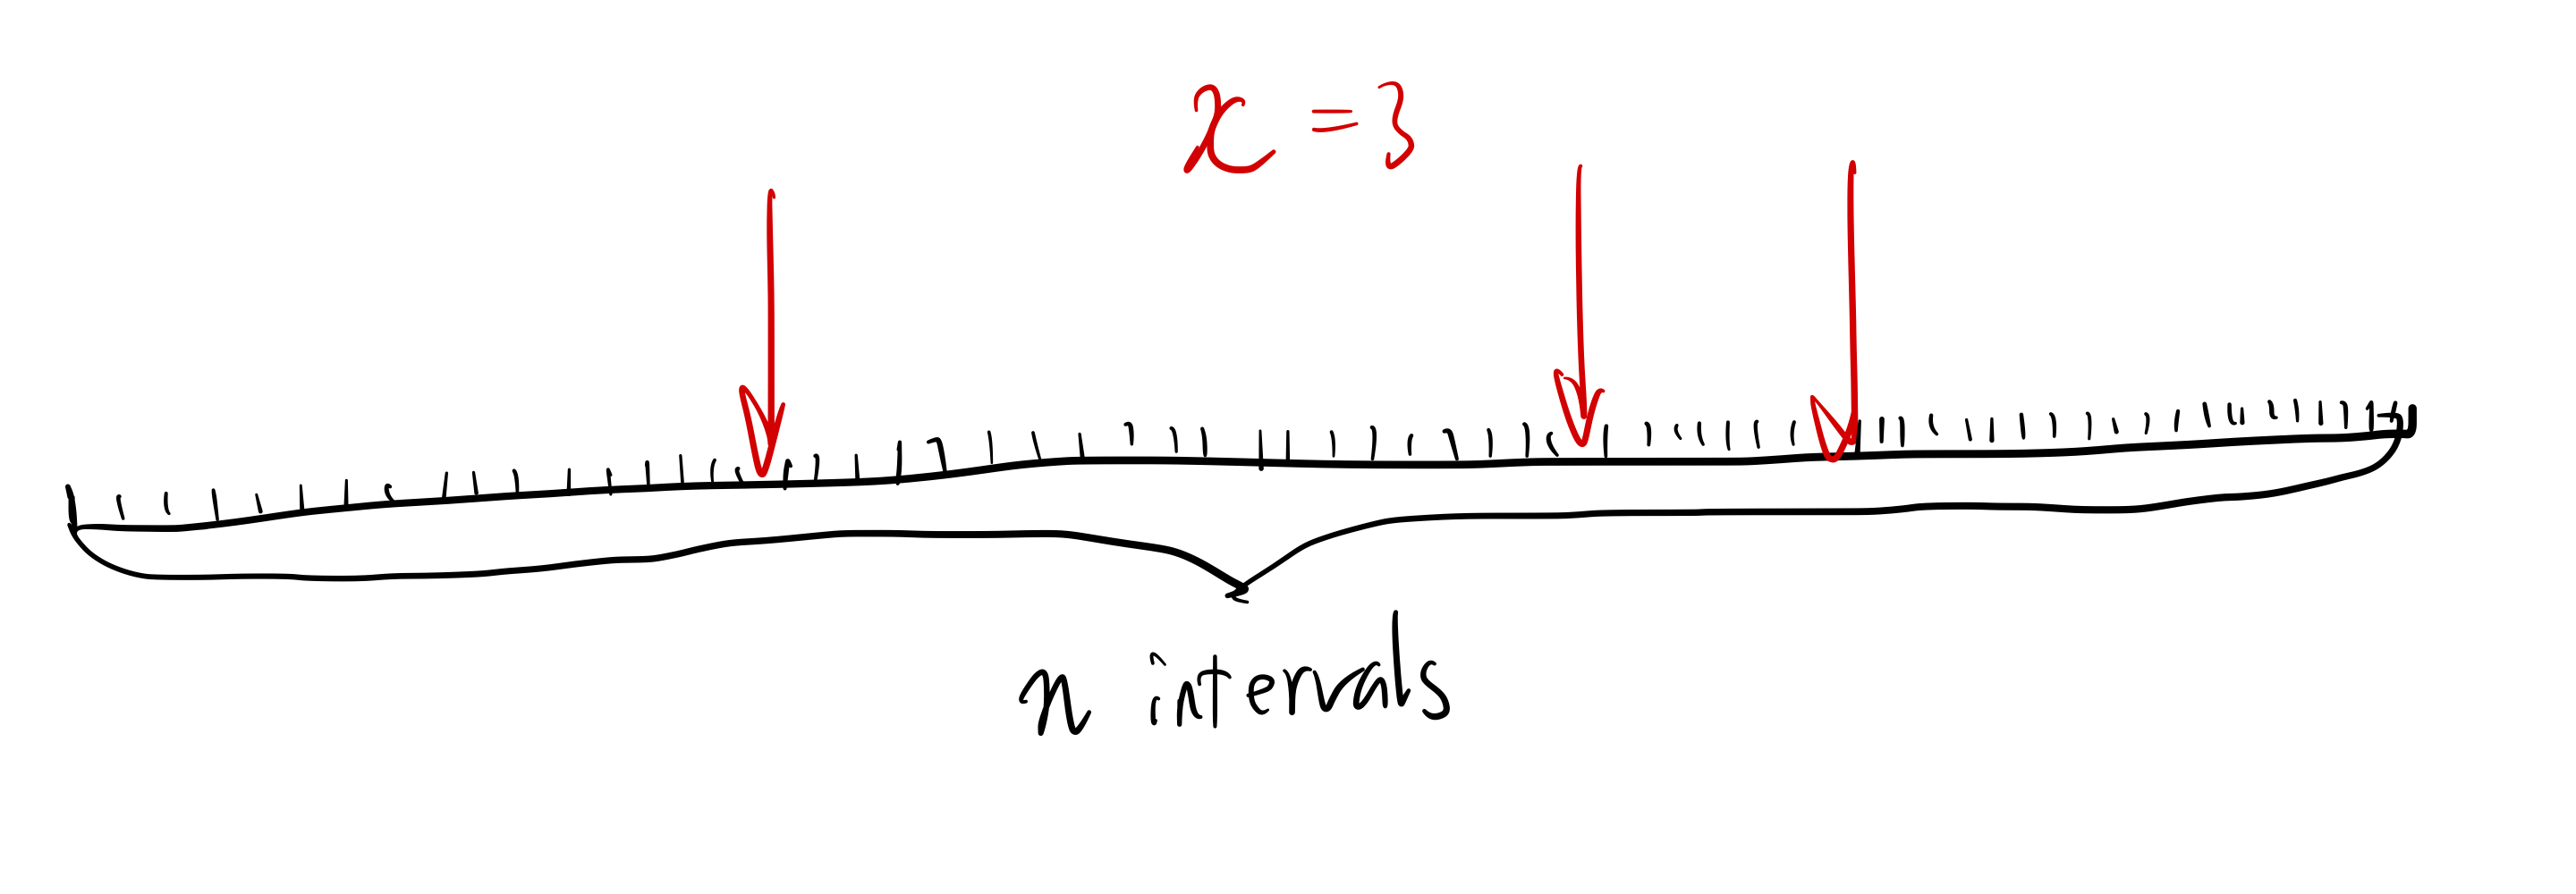
\includegraphics[width=0.7\textwidth]{figures/03-Probability_distribution/Poisson_exp.jpeg}
        \caption{以二項分布近似卜瓦松分佈}
        \label{fig:poisson_exp}
    \end{figure}

    描述次數資料最常用的分布是\textit{卜瓦松分布} (Poisson distribution),其命名來自於法國數學家 Siméon Poisson(1781-1840)。假設事件的發生滿足以下條件:(1) 發生事件之間為獨立 (2) 發生事件的頻率不隨時間點而改變 (3) 同一個時間點不會發生兩次以上的事件。那麼如圖\ref{fig:poisson_exp}所示,我們可以把追蹤的時間切成 $n$ 等分。根據上述的前兩個條件,每一等分發生事件的機率都相同且彼此獨立,而且在 $n$ 越來越大的情況下,根據第三個條件,每一個等分最多只會發生一件事件,且發生事件的機率可寫為 $\lambda/n$,其中 $\lambda$ 為在整段時間內預期發生事件的次數。整條時間線可以被看成作了 $n$ 次互相獨立、成功機率為 $\lambda/n$ 的實驗,而我們關心的是成功的總次數 $X$。在這個近似的框架下,$X$ 應該服從二項式分配,其機率質量函數可寫做
    \begin{align*}
        f_X(x) = \binom{n}{x} \Big(\frac{\lambda}{n}\Big)^x\Big(1-\frac{\lambda}{n}\Big)^{n-x} &= \frac{n (n-1)...(n-x+1)}{x!}\frac{\lambda^x}{n^x}\Big(1-\frac{\lambda}{n}\Big)^n\Big(1-\frac{\lambda}{n}\Big)^{-x}\\
        &= \frac{n (n-1)...(n-x+1)}{n^x} \Big(1-\frac{\lambda}{n}\Big)^{-x} \frac{\lambda^x}{x!} \Big(1-\frac{\lambda}{n}\Big)^n
    \end{align*}
    當切的等分數 $n$ 趨近於無窮大時,前兩項都會趨近於 $1$,而最後一項則會趨近於 $e^{-\lambda}$($e$是自然對數的底,約 2.718)。因此,卜瓦松分佈的機率質量函數為
    \[f_X(x) = \frac{\lambda^x e^{-\lambda}}{x!}, \qquad x \in \{0,1,2,3,...\}\]
    此時我們稱隨機變數 $X$ 服從速率參數 (rate parameter) $\lambda$ 的卜瓦松分布,寫作
    \[X \sim Poisson(\lambda)\]

    卜瓦松分布是一個右偏分布,如圖\ref{fig:poisson}所示,但偏度會隨著 $\lambda$ 增加而降低。根據前面用 $Binomial(n, \lambda/n)$ 二項式分佈的近似,卜瓦松分布的期望值為 $n \cdot (\lambda/n) = \lambda$。變異數則可用 $n \cdot (\lambda/n) \cdot (1- \lambda/n) = \lambda \cdot (1- \lambda/n)$ 近似,在 $n$ 趨近於無窮大時亦趨近至 $\lambda$。由此可知,卜瓦松分佈的特性為期望值和變異數相等。

    \begin{figure}[htbp]
        \centering
        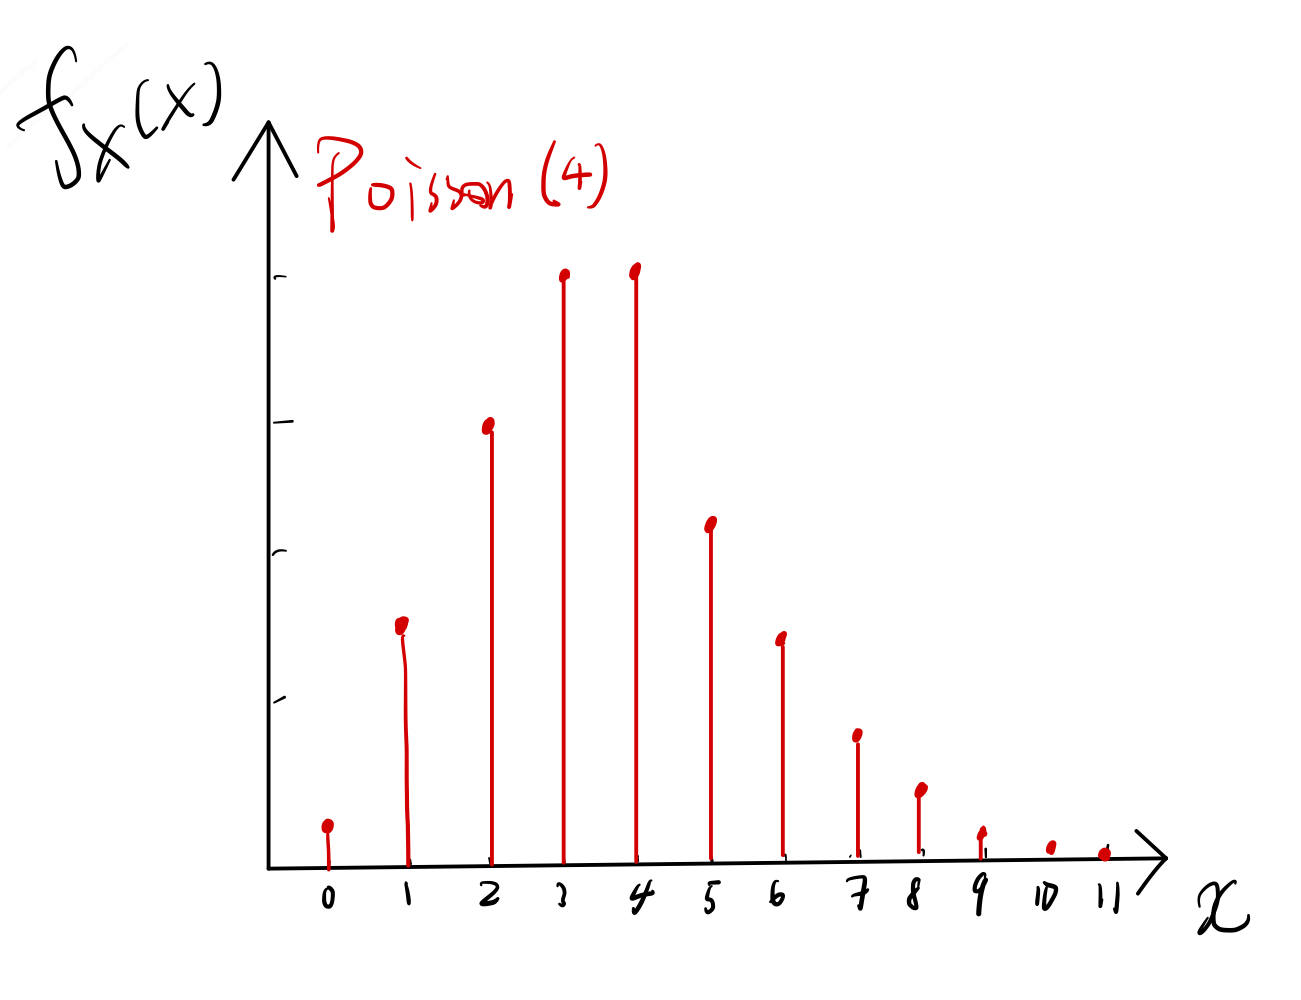
\includegraphics[width=0.6\textwidth]{figures/03-Probability_distribution/Poisson.jpeg}
        \caption{卜瓦松分佈的機率質量函數}
        \label{fig:poisson}
    \end{figure}

    \bigskip

    \begin{custom}{練習}
        根據一項大型世代研究,45 歲以上氣喘患者的平均急性發作率為一年 0.22 次。若氣喘發作的次數可用卜瓦松分配描述,那麼如何計算一位 45 歲以上氣喘患者在半年內發作兩次以上的機率?
    \end{custom}

    \bigskip

    \begin{custom}{思考}
        我們前面提到卜瓦松分佈的特性是期望值和變異數相等。如果我們抽樣的樣本並不「純粹」,而是來自多個速率參數不同的母體,那麼我們應該預期樣本變異數和樣本期望值的關係為何?
    \end{custom}

    \bigskip

    最後,我們用表\ref{tab:discrete_distribution}來總結生物醫學統計常用的離散型機率分布。
    
    \begin{table}[htbp]
        \begin{center}
            \begin{tabular}{cccc}
                \toprule
                分布名稱 & 參數 & 期望值 & 變異數\\
                \hline
                白努利 (Bernoulli) 分布 & 機率參數 $p$ & $p$ & $p(1-p)$\\
                二項式 (Binomial)分布 & 次數參數 $n$;機率參數 $p$ & $np$ & $np(1-p)$\\
                卜瓦松 (Poisson) 分布 & 速率參數 $\lambda$ & $\lambda$ & $\lambda$\\
                \bottomrule
            \end{tabular}
            \caption{生物醫學統計常用的離散型機率分布\label{tab:discrete_distribution}}
        \end{center}
    \end{table}
    
\section{連續型機率分布}

    前面我們提到,當隨機變數的可能取值可數(countable),就適合用離散型機率分布來描述,而且取得機率質量函數就完全決定了機率分布。然而,還有一類隨機變數的取值是連續而不可數的。舉例來說,如果我們在 Excel 裡輸入 \textit{RAND()} 函數,程式會隨機吐出一個 0 到 1 之間的亂數。我們把這個吐出的亂數記作隨機變數 $X$。如果小數位數無限增多,那麼從 0 到 1 之間的所有實數都是 $X$ 可能的取值,因此 $X$ 不是離散型的隨機變數,而是連續型的隨機變數,其所服從的也是一個\textit{連續型機率分布} (continuous probability distribution)。

    在連續型機率分布中,機率質量函數是沒有意義的。舉例而言,上述的 $X$ 若有機率質量函數 $f_X(x)$,則 $f_X(0.5)$ 應該代表 $X = 0.5$ 的機率。然而,$X$ 的取值是連續的,所以雖然 $X$ 可以取值 0.5,但 $X = 0.5$ 的機率等於零。事實上,$X$ 等於任何一個數的機率都等於零,所以 $X$ 的機率質量函數無法提供任何資訊。取而代之的是\textit{機率密度函數} (probability density function),如圖\ref{fig:uniform}所示。機率密度函數\textbf{曲線下的面積}代表取值區間出現的機率,例如圖中藍色的曲線下面積等於 $(0.7-0.4) \times 1 = 0.3$,代表 $X$ 取值於 0.4 到 0.7 之間的機率 $\PP(0.4 \le X \le 0.7) = 0.3$。我們也可以看到,如果區間取 「0.5 到 0.5 之間」,那麼曲線下就沒有面積,也就隱含著 $\PP(0.5 \le X \le 0.5) = \PP(X=0.5) = 0$,和我們前述單點機率等於零的結論相符。由於曲線下的面積才是機率,機率密度函數的實際取值並非機率而是\textit{機率密度} (probability density),用來度量隨機變數。也因此,雖然機率質量函數的取值不能超過 1(否則會違反總機率等於一的規則),但機率密度函數的取值卻可以超過 1,只要任何曲線下面積都不超過 1 即可。總機率等於一的規則在機率密度函數的體現,就是曲線下的總面積要等於一,寫成數學式就必須要動用到積分:
    \[\int_{-\infty}^{\infty} f_X(x) dx = 1\]
    讀者可以依此來檢查圖\ref{fig:uniform}的機率密度函數是否有符合總機率等於一的規則。
    \begin{figure}[htbp]
        \centering
        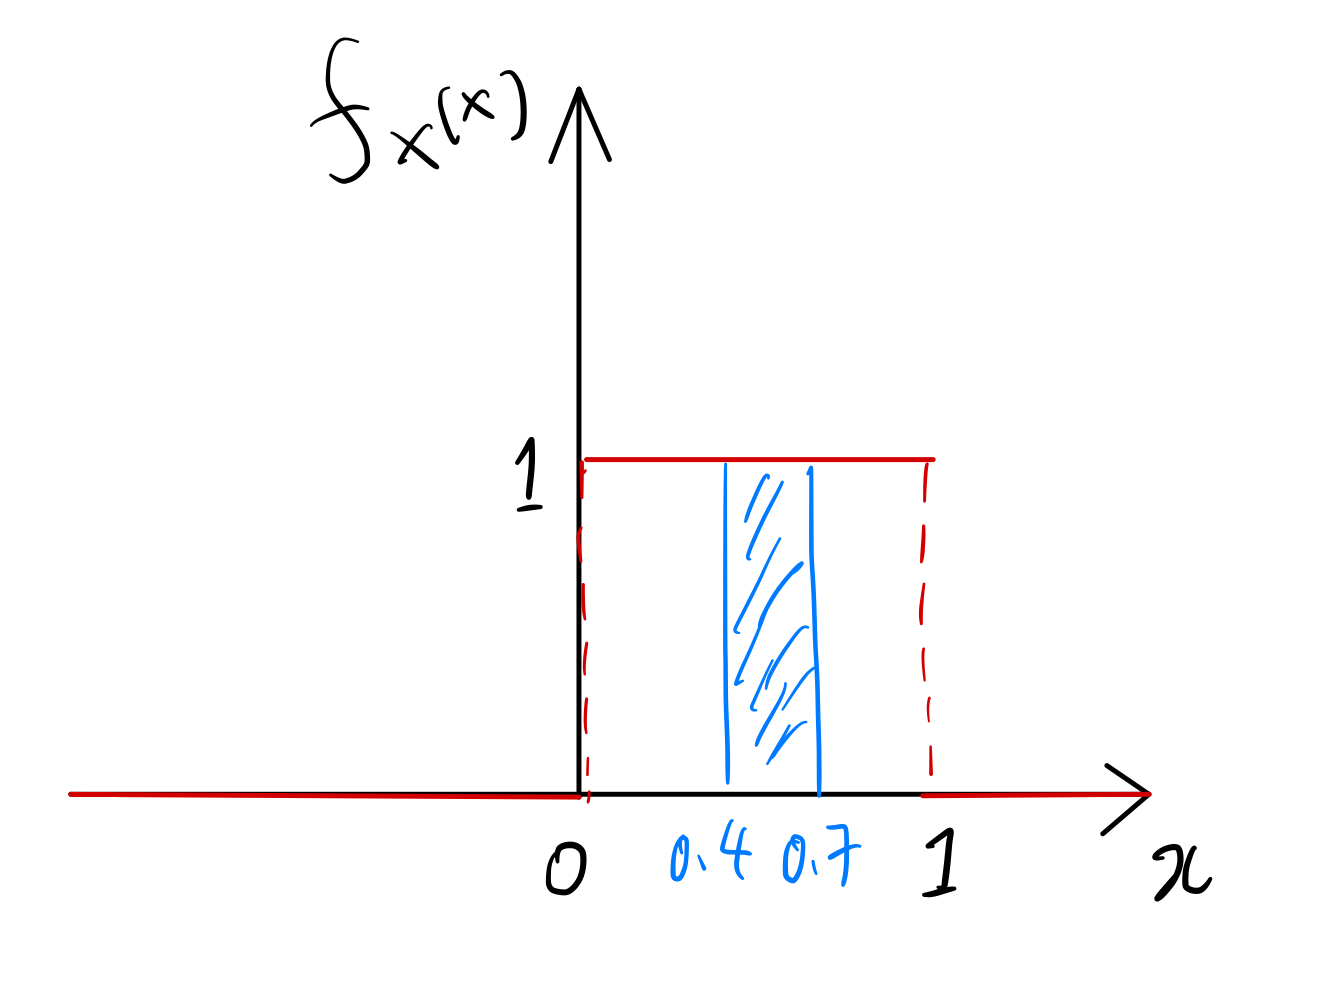
\includegraphics[width=0.6\textwidth]{figures/03-Probability_distribution/Uniform.jpeg}
        \caption{標準均一分布的機率密度函數}
        \label{fig:uniform}
    \end{figure}

    在離散型機率分布中,我們提到期望值的算法是將各取值以出現機率作加權平均,而變異數則是將「各取值與期望值距離的平方」以出現機率作加權平均。在連續型機率分布中,由於取值是連續的,我們需要將前面的定義用積分作小小的修正:
    \[\EE(X) = \int_{-\infty}^{\infty} x f_X(x) dx\]
    \[var(X) = \int_{-\infty}^{\infty} (x-\EE(X))^2 f_X(x) dx\]
    如果想要用 $var(X) = \EE(X^2) - (\EE(X))^2$ 來計算變異數,則需要用到
    \[\EE(X^2) = \int_{-\infty}^{\infty} x^2 f_X(x) dx\]

    另外,我們在離散型機率分布中提到的累積分配函數,在連續型機率分佈中仍然適用。其計算方式仍然需要用到積分:
    \[F_X(x) = \PP(X \le x) = \int_{-\infty}^x f_X(x) dx\]
    其中因為需要算出 $X \le x$ 的機率,也就是 $X$ 介於 $-\infty$ 和 $x$ 的機率,所以計算曲線下面積的積分上下限即為 $-\infty$ 到 $x$。
    
\subsection{常態分布}

    前面提到 0 到 1 之前的隨機亂數分布被稱為標準均一分布 (standard uniform distribution)。雖然標準均一分布在解釋上非常直覺,但實際上統計上最常用到的連續型分布是如圖\ref{fig:normal}左方的\textit{常態分布} (normal distribution)。常態分布又被稱為\textit{正態分布}或\textit{高斯分佈} (Gaussian distribution)。它有兩個十分直覺的參數:代表平均值的 $\mu$ 和代表變異數的 $\sigma^2$,其機率密度函數如下:
    \[f_X(x)=\frac{1}{\sqrt{2\pi\sigma^2}}e^{-\frac{(x-\mu)^2}{2\sigma^2}}\]
    當$\mu$的取值由高而低變動時,常態分布的曲線就會由右往左平移;當$\sigma^2$的取值由高而低變動時,常態分布的曲線就會由胖變瘦。此時我們稱 $X$ 服從平均值為 $\mu$、變異數為 $\sigma^2$ 的常態分布,記作
    \[X \sim Normal(\mu, \sigma^2) \qquad \text{或} \qquad X \sim \NN(\mu, \sigma^2)\]
    
    常態分布的機率密度函數雖然長得很醜陋,但常態分布是最能描述一般連續型隨機變數的分布,例如身高、體重、智商等等。從圖\ref{fig:normal}來看,常態分佈有一些重要的特徵:
    \begin{itemize}
        \item 單峰 (unimodal):常態分布最有可能取值在平均值 $\mu$ 附近。
        \item 對稱 (symmetric):常態分布以平均值 $\mu$ 為中心,左右對稱。因此,常態分布的中位數亦為 $\mu$。
        \item 鐘型 (bell-shaped):常態分佈在取值遠離平均值後,機率密度瞬間降低。事實上,我們在敘述性統計提到的經驗法則,就是由常態分布而來:常態分布取值在 $\mu \pm \sigma$ 之間的機率為 $68.2\%$;在 $\mu \pm 2\sigma$ 之間的機率為 $95.4\%$;在 $\mu \pm 3\sigma$ 之間的機率為 $99.7\%$。
    \end{itemize}

    \begin{figure}[htbp]
        \centering
        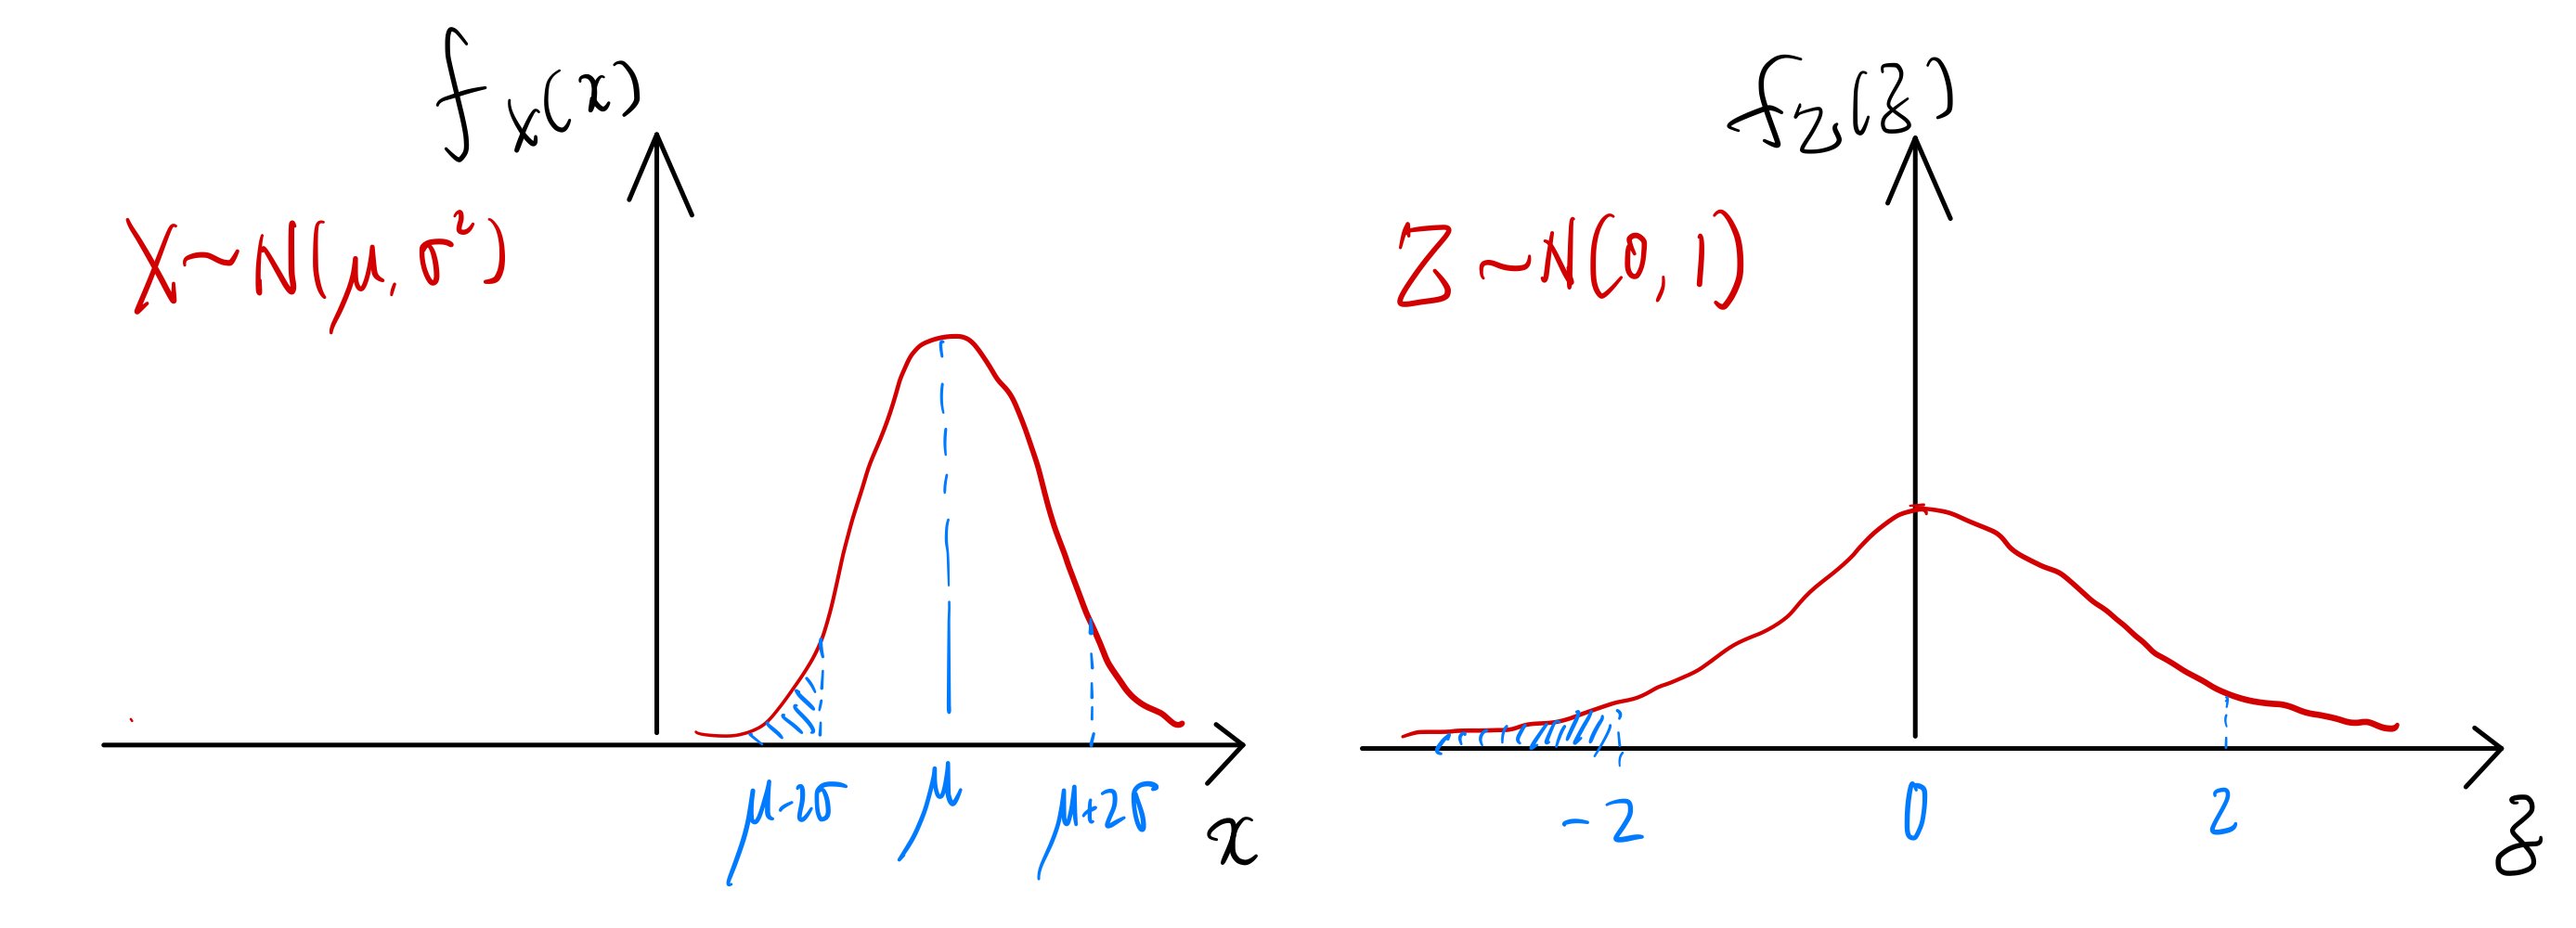
\includegraphics[width=\textwidth]{figures/03-Probability_distribution/Normal.jpeg}
        \caption{常態分布(左)與標準常態分布(右)的機率密度函數}
        \label{fig:normal}
    \end{figure}

    在所有的常態分布中,我們稱平均值$\mu =0$、變異數 $\sigma^2 = 1$的常態分布為\textit{標準常態分布} (standard normal distribution),如圖\ref{fig:normal}右方所示。其對應的隨機變數通常記為 $\ZZ$,機率密度函數則記為
    \[\phi(x)=\frac{1}{\sqrt{2\pi}}e^{-\frac{x^2}{2}}\]
    更重要的是,標準常態分布的累積分配函數常記為
    \[\Phi(x)=\int_{-\infty}^x \frac{1}{\sqrt{2\pi}}e^{-\frac{x^2}{2}} dx\]
    這個積分式只能用數值方法求值,但因為它十分重要,所以一般都會為這個函數製表,被稱為\href{https://en.wikipedia.org/wiki/Standard_normal_table}{標準常態表} (standard normal table) 或 Z 表 (Z table)。例如我們想知道 $\ZZ \ge 1.96$ 的機率,則因為常態分布是對稱的,$\ZZ \ge 1.96$ 的機率就等於 $\ZZ \le -1.96$ 的機率,查表得 $0.02500$。
    
    任何常態分布的隨機變數在經過 \textit{z轉換} (z-transform) 後都會變成標準常態分布。若 $X \sim \NN(\mu, \sigma^2)$,則
    \[\frac{X-\mu}{\sigma} \sim \NN(0,1)\]
    因此,任何常態分布的曲線下面積也都可以藉由 z 轉換求得:如果我們想知道 $X \ge x$ 的機率,那麼我們可以先算出 $x$ 經過 z 轉換後得到的 \textit{z 分數} (z-score):
    \[z = \frac{x-\mu}{\sigma}\]
    此時,我們有
    \[\PP(X \ge x) = \PP\Big(\frac{X-\mu}{\sigma} \ge \frac{x-\mu}{\sigma}\Big) = \PP(\ZZ \ge z)\]
    所以只要在標準常態表中查詢 $\ZZ \ge z$ 的機率即可。
    
    同樣的流程可以反過來做:如果我們想知道 $X$ 取值多少以上的機率為 $\alpha$,那麼我們可以先找出 $\ZZ$ 取值多少以上的機率為 $\alpha$(一般會把這個值記為 $z_\alpha$),然後我們就有:
    \[\alpha = \PP(\ZZ \ge z_\alpha) = \PP\Big(\frac{X-\mu}{\sigma} \ge z_\alpha \Big) = \PP(X \ge \mu + \sigma z_\alpha)\]
    亦即,只要把 $z_\alpha$ 視為 z 分數做反轉換,就可以找到欲求的取值閾值。
    
    \bigskip

    \begin{custom}{練習}
        假設已知清華大學的大學生身高服從一個平均值為 165 公分,標準差為 7 公分的常態分布。那麼我們預期會有多少比例的大學生身高介於 161.5 到 172 公分之間?如果我們想找出身高前 $1.5\%$ 的大學生,應該召集身高高於多少公分的學生?
    \end{custom}

    \bigskip

    \begin{custom}{練習}
        根據 WHO 定義,個人之骨質密度 T 分數 (T-score)為其骨質密度依 30-39 歲女性之骨質密度平均值與標準差作 z 轉換後所得之值。T 分數等於或低於 -2.5 者可被診斷為骨質疏鬆。假定台灣 30-39 歲女性股骨頸骨質密度之平均值及標準差為 $0.93 \pm 0.08$ g/cm$^2$、60-69 歲女性股骨頸骨質密度之平均值及標準差為 $0.76 \pm 0.15$ g/cm$^2$。若假定女性股骨頸骨質密度之分布遵從常態分布,則理論上台灣 60-69 歲女性中,有多少比例可因股骨頸骨質密度被診斷為骨質疏鬆?
    \end{custom}

    \begin{docexam}{(104-1醫學(一))}
        若已知國內男性抽菸盛行率為 $20\%$,隨機抽三位男性,三位都抽菸的機率為何?
    \end{docexam}

    \begin{docexam}{(102-1醫學(一))}
        某學生想為他這學期體育課的選課做出決定。假設一學期可選兩種運動課程,但選課人數一經額滿就無法選上。若此生選上游泳課的機率為 0.6,選上韻律課的機率為 0.5,同時選上游泳課和韻律課的機率為 0.3。此生選上韻律課或游泳課或兩種課程的機率為多少?
    \end{docexam}

    \begin{docexam}{(100-1醫學(一))}
        如果白人小孩的平均血漿醛固酮 (plasma-aldosterone) 為400 pmol/L,標準差為200 pmol/L,假設血漿醛固酮為常態分布,有多少百分比的白人小孩其血漿醛固酮$\le$ 300 pmol/L($Pr(\ZZ \ge 0.5) = 0.3085$)?
    \end{docexam}

    \begin{docexam}{(109-2醫學(二))}
        假設有一個疾病為顯性遺傳病,得病者父母親中,其中有一位有病,另一位則無。這種疾病每位子女遺傳的機率 $1/2$,一個有 2 個小孩的家庭,兩個小孩皆得病的機率為何?
    \end{docexam}
\chapter{抽樣分布與中央極限定理}
    我們在第三章中提到,做實驗或是抽樣時得到的結果具有隨機性,因此可以用隨機變數來代表,並用背後的機率分布來描述之。隨機變數的觀察值即為由其分布隨機抽出的\textbf{一個}數值。例如,那麼隨機抽取\textbf{一位}學生所得到的身高(以公分為單位)可以用隨機變數 $X$ 表示,且可以假定 $X$ 服從某個常態分布。然而,在實際收集及分析資料時,我們關注的通常不是一個觀察值,而是會抽取一組樣本並得到\textbf{一群}觀察值,並這群觀察值計算出我們有興趣的量。例如,我們可能抽出了 $50$ 位大學生測量身高,並計算他們的的身高平均值。這個平均值依然具有隨機性(抽出不同的同學,得到的平均身高就會不一樣),因此也可以用隨機變數來表示,例如 $\bar{X}$。此時如果我們要用這個身高平均值來做統計推論,就要了解 $\bar{X}$ 背後的機率分布為何。我們將在這章說明統計量抽樣分布的概念、樣本平均抽樣分布的性質,以及如何統計中最重要的\textbf{中央極限定理}來描述樣本平均的抽樣分布。
    
    \begin{introduction}[第 \thechapter 章學習目標]
        \item 了解抽樣分布的意義以及其與母體分布的不同
        \item 樣本平均抽樣分布的性質
        \item 中央極限定理的意義、適用範圍與應用
    \end{introduction}

\section{抽樣分布}
    假設清華大學的大學生身高服從一個平均值為 165 公分,標準差為 7 公分的常態分布。在前一章我們說過,如果把抽取一位學生得到的身高(以公分為單位)記作隨機變數 $X$,那麼我們可以寫作 $X \sim \NN(165, 7^2)$。這代表我們抽取一位學生測量身高時,相當於從 $\NN(165,7^2)$ 這個分布抽取一個數字。換句話說,如果我們重複地「抽取一位學生並測量身高」,那麼所得身高觀察值的分布將會如圖\ref{fig:sampling_mean}最左邊的直方圖。

    \begin{figure}[htbp]
        \centering
        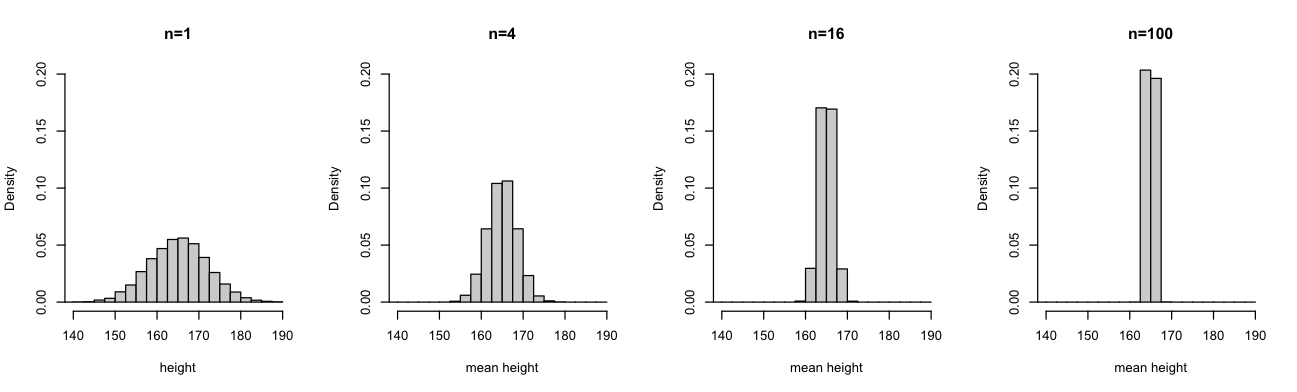
\includegraphics[width=\textwidth]{figures/04-Sampling_distribution_CLT/sampling_mean.png}
        \caption{身高平均值的抽樣分布}
        \label{fig:sampling_mean}
    \end{figure}

    現在假設我們隨機抽取了 4 位學生並測量身高。此時我們有 4 位學生,所以共有 4 個身高,但是這四個身高不能都用 $X$ 來表示(否則就隱含著四位學生身高均等),因此我們可以用 $X_1, X_2, X_3, X_4$ 來代表這 4 個身高對應的隨機變數。這 4 個隨機變數都服從 $N(165, 7 ^2)$ 的分配,而且互相獨立,所以我們可以寫作
    \[X_1 \sim \NN(165, 7^2)\;\; ; \;\;X_2 \sim \NN(165, 7^2)\;\; ;X_3 \sim \NN(165, 7^2)\;\; ;X_4 \sim \NN(165, 7^2)\;\;\]
    \[X_1,X_2,X_3,X_4\text{ 相互獨立 (mutually independent)}\]
    這種分布相同又相互獨立的情境在隨機抽樣中很常見,統計中給它一個專有名詞:\textit{獨立同分布} (independent and identically distributed),簡寫為 iid。因此,我們也可以寫為
    \[X_1, X_2, X_3, X_4 \overset{\text{iid}}{\sim} \NN(165, 7^2)\]
    此時如果我們計算身高的平均值並令其為隨機變數 $\bar{X}$,則 $\bar{X}$ 可以寫成:
    \[\bar{X} = \frac{X_1+X_2+X_3+X_4}{4}\]
    可以看到 $\bar{X}$ 是由樣本 $X_1,X_2,X_3,X_4$ 計算而得的隨機變數。這種不含未知參數、由樣本計算出的隨機變數在統計中被通稱為\textit{統計量} (statistic)。由於統計量是由隨機變數算出,它也會具有不確定性,也就是背後有一個分布。這個分布被稱為統計量的\textit{抽樣分布}(sampling distribution)。類似前面我們所說,我們抽取 4 位學生並算出平均身高時,相當於從 $\bar{X}$ 的抽樣分布抽取一個數字。換言之,如果我們重複地「抽取 4 位學生並計算平均身高」,所得平均身高的分布即為 $\bar{X}$ 的抽樣分布,如圖\ref{fig:sampling_mean}的左二直方圖。可以看到,\textbf{統計量的抽樣分布和樣本的機率分布是完全不一樣的},讀者一定要避免混淆。另外,如果我們不是抽取 4 位,而是抽取 16 位或 100 位學生來計算平均身高,則平均身高的抽樣分布如圖\ref{fig:sampling_mean}的右邊二個直方圖。可以看到,雖然都是平均值,但是抽取 4 位、16 位和 100 位學生計算出之平均值的抽樣分布都不一樣,因此樣本數也會影響統計量的抽樣分布。
    
    統計量的定義為「樣本計算出的隨機變數」,並不限於樣本平均,因此我們也可以建構其他統計量的抽樣分布:如果我們抽取 4 位、16 位或 100 位學生來計算身高樣本變異數,其抽樣分布則如圖\ref{fig:sampling_var}。可以看到這些抽樣分布均為右偏分布,和平均值的抽樣分布非常不同。總結來說,\textbf{統計量的種類和樣本數均可能影響抽樣分布的型態}。

    \begin{figure}[htbp]
        \centering
        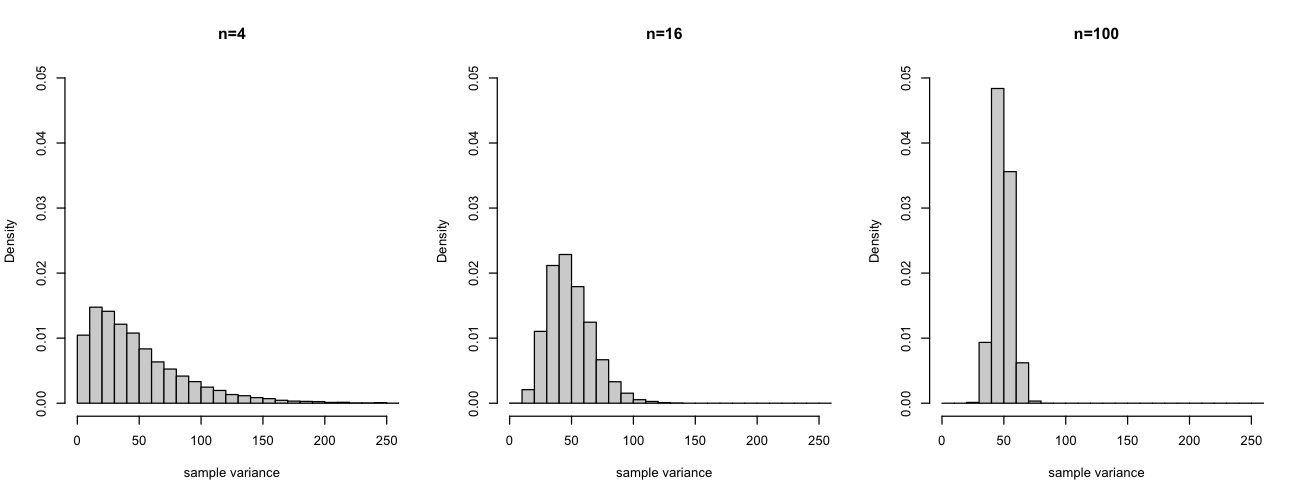
\includegraphics[width=\textwidth]{figures/04-Sampling_distribution_CLT/sampling_var.png}
        \caption{身高樣本變異數的抽樣分布}
        \label{fig:sampling_var}
    \end{figure}

    抽樣分布作為一個機率分布,也是可以計算期望值、變異數和標準差。其中統計量抽樣分布的標準差又被稱為統計量的\textit{標準誤} (standard error)。當統計量是用來估計母體參數時(例如樣本平均估計母體平均、樣本變異數估計母體變異數),統計量又被稱為\textit{估計量}(estimator),其觀察值則被稱為\textit{估計值} (estimate)。由於估計量具有變異性,估計值恰好等於母體參數的機會很低,但是我們可以藉由估計量的抽樣分布來考察估計值的表現。其中,估計量的期望值和標準誤是最直覺且重要的兩個評估點。
    
    如果估計量抽樣分布的期望值等於母體參數,代表估計值的取值會以母體參數為中心,我們就會比較信任這個估計量。這種估計量被稱為\textit{不偏估計量} (unbiased estimator)。例如在圖\ref{fig:sampling_mean}的左二圖中,如果我們用「四個學生的平均身高」作為清華大學生平均身高的估計量,可以看到這個估計量的抽樣分布平均值是 165,和母體平均相同,因此該估計量是不偏估計量。用符號來說,如果要估計的母體參數為 $\theta$,而我們提出的估計量是 $\hat{\theta}$,則 $\EE(\hat{\theta}) = \theta$ 時,$\hat{\theta}$ 為 $\theta$ 的不偏估計量。我們先前提到的樣本平均值、樣本變異數都是母體平均值、母體變異數的不偏估計量。

    估計量的標準誤代表了估計量取值的分散程度。當估計量為不偏時,雖然估計值雖然以母體參數為中心取值,但距離母體參數的遠近則不一定。例如圖\ref{fig:sampling_mean}中間的兩個圖中,「抽樣 4 位學生取身高平均」和「抽樣 16 位學生取身高平均」都是清華大學生身高平均值的不偏估計量,但是前者較可能出現 175, 155 這種偏離較多的估計值,後者則大多分布在 160 到 170 之間。因此,估計量的標準誤對於其估計精確程度也有影響。一般而言,我們希望估計量能夠不偏,又有很小的標準誤,這樣估計值就會非常接近母體參數。

    \bigskip
    
    \begin{custom}{思考}
        假設在清華大學生的例子中,我們抽樣 4 個人,並令 4 個人中最矮的人的身高為 $X_{(1)}$(以公分為單位)。請問 $X_{(1)}$ 是否為統計量?如何用重複抽樣的方式來畫出 $X_{(1)}$ 的抽樣分布?如果拿 $X_{(1)}$ 來估計清華大學生的平均身高,你覺得 $X_{(1)}$ 是否為不偏估計量?
    \end{custom}

    \bigskip

    \begin{custom}{思考}
        同樣是清華大學生的例子中,如果我們抽樣 100 個人並算出身高樣本變異數 A,然後再抽樣 250 個人並算出身高樣本變異數 B。那麼這兩個樣本變異數:(1) 都是估計母體的變異數,所以一般而言A、B數值會相近 (2) 是在估計平均值的標準誤,所以一般而言 A<B (3) 是在估計平均值的標準誤,所以後者一般而言 A>B。
    \end{custom}

    \bigskip

    \begin{custom}{思考}
        再次使用清華大學生的例子。如果我們隨機找一位學生,然後就用他的身高當成清華大學生平均身高的估計量。請問這個估計量是否為不偏估計量?
    \end{custom}
    
\section{樣本平均的抽樣分布}

    在各種統計量中,最常用的統計量就是樣本平均。因此,我們這裡針對樣本平均的統計性質作特別探討。假設我們從一個平均值為 $\mu$、變異數為 $\sigma^2$ 的母體抽出樣本數為 $n$ 的一組獨立樣本,得到的觀察值分別記為 $X_1, X_2, ..., X_n$。此時 $X_1, X_2, ..., X_n$ 為獨立同分布,期望值均為 $\mu$,變異數均為 $\sigma^2$。樣本平均可寫為
    \[\bar{X} = \frac{X_1 + X_2 + ... + X_n}{n} = \frac{1}{n}\sum_{i=1}^n X_i\]
    我們之前有學到隨機變數經過線性轉換後期望值和變異數的變化。我們來用這些先備知識來計算樣本平均的期望值。
    \begin{align*}
        \EE(\bar{X}) &= \EE\Big(\frac{X_1 + X_2 + ... + X_n}{n}\Big)&\\
        &= \frac{1}{n}\EE(X_1 + X_2 + ... + X_n)&\text{(縮放的期望值等於期望值縮放)}\\
        &= \frac{1}{n}[\EE(X_1) + \EE(X_2) + ... + \EE(X_n)]&\text{(相加的期望值等於期望值相加)}\\
        &= \frac{1}{n}[\mu + \mu + ... + \mu]&\text{(}X_i\text{獨立同分布,期望值為}\mu\text{)}\\
        &= \frac{1}{n}[n\mu] = \mu&\\
    \intertext{因此,\textbf{樣本平均是母體平均的不偏估計量}。接下來我們來計算樣本平均的變異數。}
        var(\bar{X}) &= var\Big(\frac{X_1 + X_2 + ... + X_n}{n}\Big)&\\
        &= \frac{1}{n^2}var(X_1 + X_2 + ... + X_n)&\text{(縮放的變異數等於變異數縮放平方倍)}\\
        &= \frac{1}{n}[var(X_1) + var(X_2) + ... + var(X_n)]&\text{(獨立隨機變數相加的變異數等於變異數相加)}\\
        &= \frac{1}{n}[\sigma^2 + \sigma^2 + ... + \sigma^2]&\text{(}X_i\text{獨立同分布,變異數為}\sigma^2\text{)}\\
        &= \frac{1}{n}[n\sigma^2] = \frac{\sigma^2}{n}&
    \end{align*}
    可以看到,\textbf{樣本平均的變異數是母體變異數除以樣本數}。把兩邊同時開根號後,我們得到
    \[sd(\bar{X}) = \frac{\sigma}{\sqrt{n}}\]
    因此,\textbf{樣本平均的標準誤是母體標準差除以根號樣本數}。因為樣本平均的標準誤太常用了,統計上給它一個專有名詞\textit{平均值標準誤} (standard error of the mean, SEM)。上述結果顯示,隨著樣本數增多,樣本平均對於母體平均的估計越來越精準,而且標準誤跟樣本數開根號呈反比。更進一步來說,當樣本數趨近於無窮大,平均值標準誤將會無限靠近零,也就是樣本平均會無限靠近母體平均。這個現象就是著名的\textit{大數法則} (Law of Large Numbers):只要樣本是獨立同分布,隨著樣本數增至無窮大,樣本平均終究會(機率)收斂至母體平均。

    注意到這裡我們在描述母體時,並沒有說它是什麼分布,而只說了它的平均值為 $\mu$、變異數為 $\sigma^2$。因此,母體分布是連續型或離散型、左偏右偏或對稱並不影響我們的結論。例如於圖\ref{fig:mean_dist_bern}中,我們假設母體為機率參數 0.64 的白努利分布,機率質量函數的型態如左上角。其平均值為 $0.64$,標準差為 $\sqrt{0.64*0.36} = 0.48$。右上、左下、右下分別是樣本數為 4、25、100 的樣本平均抽樣分布。其中可以看到樣本數為 4 時只有五種可能取值,因為樣本平均為四個白努利隨機變數的平均,也就是這四次白努力實驗成功次數除以 4,可能的取值就只有 0/4、1/4、2/4、3/4、4/4 這五種。圖中樣本平均抽樣分布的平均值均在 $0.6$,也就是白努利分布的平均值。標準誤則隨著樣本數增加而逐漸降低(分布逐漸變窄),且我們可以精確的算出各樣本數下的平均值標準誤。當 $n=4$ 時,標準誤應為 $\frac{0.48}{\sqrt{4}} = 0.12$、當$n=100$時,標準誤應為$\frac{0.48}{\sqrt{100}} = 0.048$。這種期望值不變,標準誤下降的現象在其他分布也同樣會出現,圖\ref{fig:mean_dist_unif}即用連續型的標準均一分布作為母體。

    \begin{figure}[htbp]
        \centering
        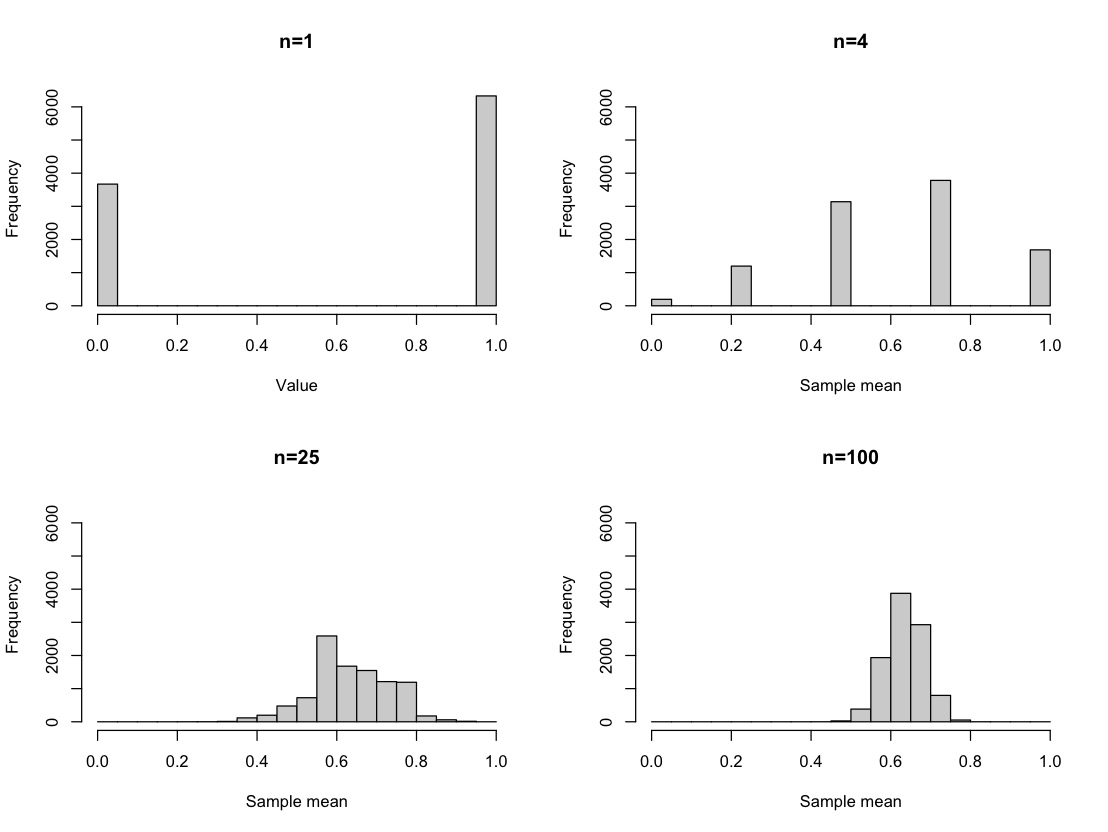
\includegraphics[width=0.9\textwidth]{figures/04-Sampling_distribution_CLT/mean_dist_bern.png}
        \caption{母體為 $Bernoulli(0.6)$ 的樣本平均抽樣分布}
        \label{fig:mean_dist_bern}
    \end{figure}

    \begin{figure}[htbp]
        \centering
        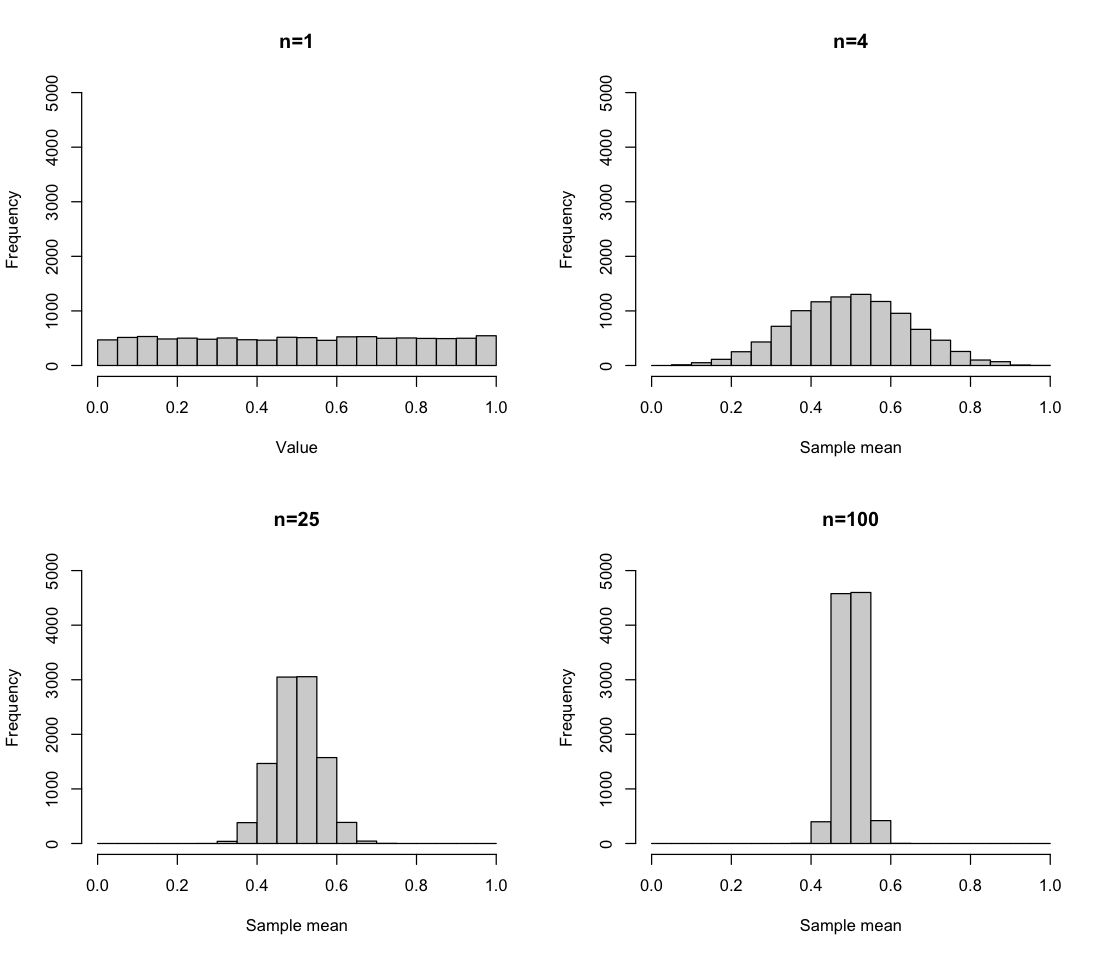
\includegraphics[width=0.9\textwidth]{figures/04-Sampling_distribution_CLT/mean_dist_unif.png}
        \caption{母體為標準均一分布的樣本平均抽樣分布}
        \label{fig:mean_dist_unif}
    \end{figure}

    一個特殊情況是,\textbf{當母體服從常態分布時,樣本平均也會服從常態分布}。由於常態分布只有兩個參數:平均值和變異數,而我們已知樣本平均的期望值是 $\mu$,變異數是 $\sigma^2/n$,所以我們可以直接寫出樣本平均的分布
    \[\bar{X} \sim \NN\Big(\mu, \frac{\sigma^2}{n}\Big)\]
    舉例而言,如果已知 60-70 歲男性的收縮壓 (mmHg) 分布服從 $\NN(130, 10)$ 的常態分布,那麼抽樣 16 位 60-70 歲男性算出的平均收縮壓就應該服從 $\NN(130, 10/\sqrt{16} = 2.5)$。我們還能依此算出平均收縮壓介於某個區間的機率,例如該平均收縮壓介於 125 至 135 mmHg 的機率為
    \[\PP(125 \le \bar{X} \le 135) = \PP\Big(\frac{125-130}{2.5} \le \frac{\bar{X}-130}{2.5} \le \frac{125-130}{2.5}\Big) = \PP(-2 \le \ZZ \le 2) \approx 0.954\]
    
    \bigskip

    \begin{custom}{練習}
        假設我們從平均值為 150 、標準差為 5 的母體抽出一個樣本數為 25 的樣本,則樣本標準差應該會最接近下列哪個數值:(1) 5 (2) 1 (3) 1/5。
    \end{custom}

    \bigskip

    \begin{custom}{練習}
        根據一項大型世代研究,45 歲以上氣喘患者的平均急性發作率為一年 0.22 次。假設一年氣喘的發作次數可用卜瓦松分布來描述。現由 45 歲以上氣喘患者中隨機抽取 100 人並計算他們平均一年氣喘發作的次數。該平均次數的期望值和標準誤應為何?
    \end{custom}

    \bigskip

    \begin{custom}{練習}
        回到清華大學生的例子。假設我們不知道清華大學生身高的分布,因此隨機抽取了三位學生來量身高,分別是 160、165、170 公分,並得到樣本平均值 165 公分以估計母體平均。請問我們是否知道該樣本平均的標準誤確切數值?若否,如何用資料來估計該樣本平均的標準誤?
    \end{custom}

    \bigskip

    \begin{custom}{思考}
        在醫學流病的應用研究中,通常會有製作一個 Table 1 來描述納入族群的特徵,例如性別比例、年齡、慢性病史比例等等。針對連續型變項例如年齡,假設樣本平均為 55 歲,樣本標準差為 10 歲,樣本數為 100 人,那麼年齡的敘述性統計應該寫成 $55 \pm 10$ (正負標準差)比較合理,還是 $55 \pm 1$ (正負標準誤)比較合理?
    \end{custom}
    
\section{中央極限定理}
    我們前面探討平均值抽樣分布的性質時,僅關注了它的期望值和標準差(即平均值標準誤),並且知道母體為常態分布時,樣本平均亦服從常態分布。然而,當母體非常態分布時,我們對於樣本平均的分布形狀並未著墨。觀察圖\ref{fig:mean_dist_bern}和\ref{fig:mean_dist_unif}可以看到,當樣本數比較少(n = 4, 25)的時候,平均值抽樣分布的型態較為取決於母體分布。例如母體為左偏的白努利分布時,平均值抽樣分布還是有點離散,而且大致上是左偏。不過當樣本數變大時(n = 100),兩個母體分布下的樣本平均抽樣分布都呈現大致對稱的鐘型。這個鐘型分布不是別的分布:正是常態分布!\textbf{不論母體分布為何},只要樣本數不斷增大,樣本平均抽樣分布都會趨近於常態分布。由於常態分布只有兩個參數:平均值與變異數,而我們在前一節已經導出樣本平均抽樣分布的平均值(母體平均)與變異數(母體變異數除以樣本數),所以這個趨近的常態分布就完全已知了。以上就是統計中最重要的\textit{中央極限定理} (Central Limit Theorem, CLT):

    \begin{theorem*}{(中央極限定理)}
        若 $X_1, X_2, ... X_n$ 為獨立同分布、平均值為 $\mu$、變異數為 $\sigma^2$ 的隨機變數,令樣本平均 $\bar{X} = \frac{1}{n}\sum_{i=1}^n X_i$,則當 $n \rightarrow \infty$
        \[\frac{\bar{X}-\mu}{\sigma/\sqrt{n}} \xrightarrow[]{d} \NN(0,1)\]
        或是用比較不嚴謹的寫法
        \[\bar{X} \xrightarrow[]{d} \NN\Big(\mu,\frac{\sigma^2}{n}\Big)\]
    \end{theorem*}
    中央極限定理精要就是\textbf{任何母體的樣本平均抽樣分布,在樣本「夠大」的情況下,會趨近於常態分布}。至於怎樣才叫「夠大」,理論上要視母體分布的偏斜和厚尾程度而定,但一般會認為樣本數大於 30 就足夠讓我們用常態分布來\textbf{近似}平均值抽樣分布。
    
    利用中央極限定理,我們就可以寫出更多估計量的近似分布,進而計算出估計量在指定區間的機率。例如,如果我們做一份 $n$ 人的民調,調查對於某議案的支持度,那麼每個民調受訪者是否支持其實都服從一個機率參數為 $p$ 的白努利分布,其中 $p$ 為全民對該議案的支持度。民調最後顯示的支持度 $\hat{p}$ 即為這些白努利分布隨機變數的平均值,因此根據中央極限定理,因為白努利分布的期望值為 $p$、變異數為 $p(1-p)$,我們有
    \[\hat{p} \xrightarrow[]{d} \NN\Big(p, \frac{p(1-p)}{n}\Big)\]
    因此,一個實際支持率為 $60\%$ 的議案,若做一份 $600$ 人的民調,其民調支持率 $\hat{p}$ 應趨近服從 $\NN(0.6, \frac{0.6 \cdot 0.4}{600} = 0.0004)$。根據這個近似抽樣分布,民調支持率低於 $55\%$ 的機率可以如下計算:
    \[\PP(\hat{p} \le 0.55) = \PP\Big(\frac{\hat{p}-0.6}{\sqrt{0.0004}} \le \frac{0.55-0.6}{\sqrt{0.0004}}\Big) \approx \PP(\ZZ \le -2.5) \approx 0.00621\]
    注意到如果我們把民調支持率乘上樣本數,就會得到支持人數。根據平均值與變異數的性質,支持人數 $Y$ 的近似分配可寫為
    \[Y = n\hat{p} \xrightarrow[]{d} \NN(np, np(1-p))\]
    先前我們提到過支持人數應該是遵從次數參數為 $n$、機率參數為 $p$ 的二項式分布,而這裡顯示支持人數在民調人數大時,趨進於上述的常態分布。這意味著二項式分布在次數參數 $n$ 足夠大的時候,可以用平均值與變異數相仿的常態分布來近似。至於怎樣叫作「足夠大」,一般認為 $np$ 和 $n(1-p)$ 均大於 $10$ 的時候近似效果就很好。同樣地,由於卜瓦松分布是二項式分布在 $np=\lambda$ 且 $n$ 趨近無限大時的分布,所以當 $\lambda > 10$ 時,我們也可以用 $\NN(\lambda, \lambda)$ 來近似卜瓦松分布。

    使用常態分布近似二項分布或卜瓦松分布時,為了讓近似更加準確,經常會引進\textit{連續性校正} (continuity correction),也就是把 $\PP(X = x)$ 的機率用常態分布中的 $\PP(x-0.5 \le X \le x + 0.5)$ 來近似。舉例來說,如果 $X \sim Poisson(36)$,且我們想計算 $32 \le X \le 37$ 的機率。因為速率參數已經大於 10,我們可以試著用 $\NN(36, 36)$ 來近似 $X$ 的分布。此時 $32 \le X \le 37$ 的機率,套用連續性校正後變成求 $31.5 \le X \le 37.5$ 的機率,因此計算如下
    \begin{align*}
        \PP(31.5 \le X \le 37.5) &= \PP\Big(\frac{31.5-36}{\sqrt{36}} \le \frac{X-36}{\sqrt{36}} \le \frac{37.5-36}{\sqrt{36}}\Big)\\
        &\approx \PP(-0.75 \le \ZZ \le 0.25) \approx (1-0.401)-0.227 = 0.372
    \end{align*}
    如果實際用卜瓦松分布的機率質量函數計算 $\PP(32 \le X \le 37) = \sum_{j=32}^{37} \frac{36^j e^{-36}}{j!} \approx 0.378$,可見近似的效果還不錯。除了用來作統計量的分布近似外,中央極限定理在推論統計的其他工具中扮演了舉足輕重的角色。我們會在未來的課程中不斷使用這個重要的定理。

    \bigskip

    \begin{custom}{練習}
        根據研究,服用降低血脂的 statin 類藥物出現嚴重肌病變的機率約為五千分之一。台灣的糖尿病與高血壓患者約有八萬五千人正在接受 statin 類藥物治療,試計算出現嚴重肌病變人數在 25 人以上的機率。
    \end{custom}

    \begin{docexam}{(107-2醫學(二))}
        下列何者不是中央極限定理的涵義?
        
        (A) 隨機樣本平均值之統計分布接近常態分布
        
        (B) 隨機樣本平均值之統計分布接近布阿松分布 (Poisson distribution)
        
        (C) 所有可能的隨機樣本平均值之平均值等於母群體平均值
        
        (D) 標準誤取決於母群體標準差與樣本的大小
    \end{docexam}

    \begin{docexam}{(105-2醫學(一))}
        下列對中央極限定理的描述,何者錯誤?
        
        (A) 只要樣本數夠大,無論原本母群體是否為常態分布,樣本平均值的抽樣分布會接近常態分布
        
        (B) 母群體的平均值若為 $\mu$,則樣本平均值抽樣分布的平均值為 $\mu$
        
        (C) 母群體的標準差若為 $\sigma$,則樣本平均值抽樣分布的標準差為 $\sigma/n$
        
        (D) 可透過中央極限定理將樣本平均值的抽樣分布變成標準常態分布
    \end{docexam}

    \begin{docexam}{(104-1醫學(一))}
        下列對中央極限定理的敘述,何者錯誤?
        
        (A) 只要樣本數夠大,樣本平均數的分布就會趨近常態分布
        
        (B) 只要樣本數夠大,樣本平均數分布的期望值就會很接近母體平均數
        
        (C) 只要樣本數超過 1,樣本平均數分布的標準差都會小於母體標準差
        
        (D) 母體分布只有在常態分布時,樣本數夠大時樣本平均數的分布才會趨近常態分布
    \end{docexam}

    \begin{docexam}{(103-2醫學(一))}
        一個等距尺度之臨床變數為雙峰分布,以大樣本經過多次重複抽樣之後,其樣本平均數的抽樣分布為一個常態分布。此現象反應下列何種定理?
        
        (A) 中央極限定理
        
        (B) 貝氏定理
        
        (C) 機率總和定理
        
        (D) 二項式定理
    \end{docexam}

    \begin{docexam}{(103-1醫學(一))}
        當樣本統計量與母群體母數之差的平均值為0,亦即統計量的期望值等於母數。此統計量具有下列何種統計學特性?
        
        (A) 有效性
        
        (B) 一致性
        
        (C) 充分性
        
        (D) 不偏性
    \end{docexam}

    \begin{docexam}{(102-2醫學(一))}
        下列對中央極限定理的敘述何者錯誤?
        
        (A) 樣本平均數之抽樣分布的標準差又稱標準誤,其值等於樣本標準差除以樣本數
        
        (B) 樣本平均數之抽樣分布的平均值等於母體平均值
        
        (C) 如果母群體為常態分布,即便樣本數不大,樣本平均數之抽樣分布也會接近常態分布
        
        (D) 如果樣本數夠大,則樣本平均數之抽樣分布定會接近常態分布
    \end{docexam}
\chapter{推論統計:區間估計}

    統計中對於未知參數的估計方法有兩種:\textit{點估計} (point estimation) 和\textit{區間估計} (interval estimation)。其中點估計較為直觀,即利用樣本求出一個統計量(稱為估計量)來估計未知參數。我們在第二章已經提到了針對母體平均與母體變異數的最佳點估計量(即樣本平均與樣本變藝術),並在第四章中提到評估點估計量時需要知道估計量的抽樣分布,以了解該估計量是否不偏,以及該估計量的標準誤多大。
    
    在這一章,我們將會深入探討參數的另一類估計方法:區間估計。我們將從平均值區間估計的建構方式出發,了解樣本平均的抽樣分布在區間估計扮演的角色,以及如何正確解釋區間估計隱含的機率敘述。
    
    \begin{introduction}[第 \thechapter 章學習目標]
        \item 了解估計的兩種型式:點估計和區間估計
        \item 了解信賴區間的解釋意義
        \item 計算母體為常態分布下平均值的信賴區間
        \item 計算母體為其他分布下平均值的信賴區間
    \end{introduction}

    點估計是用一個數值來估計母體參數,因此我們需要額外用估計值的標準誤來量化點估計的不確定性。區間估計則是利用區間來估計參數,例如「我們有 95\% 的信心,清華大學生的平均身高將被 (160, 170) 公分這個區間覆蓋。」這樣的估計方法雖然沒有明確指出一個估計值,但是同時告知了估計的約略位置以及不確定性,因此被稱為區間估計。
    
    建構區間估計的其中一種方法是先尋找一個含未知參數、但分布已知的量(這在統計中被稱為樞紐量 (pivotal quantity))。例如,如果我們在某種狀況下已知清華大學生的身高標準差為 5 公分,但是不知道母體平均值為何。這時候我們抽了 36 位學生得到平均身高為 $\bar{X}$ 公分,則根據前一章所述,若母體平均值為 $\mu$ 公分,則 $\bar{X}$ 的抽樣分布為
    \[\bar{X} \sim \NN\Big(\mu, \frac{5^2}{36}\Big)\]
    此時可以發現,將 $\bar{X}$ 作 z 轉換,就可以得到一個服從標準常態分布的樞紐量:
    \[\frac{\bar{X} - \mu}{5/\sqrt{36}} \sim \ZZ\]
    如果我們此時想得到 $95\%$ 信心的區間估計,可以先從以下的等式出發,建構出一個以 0 為中心左右對稱,且機率為 $95\%$ 的區間:
    \[\PP(-z_{0.025} < \ZZ < z_{0.025}) = 1-2 \times 0.025 = 0.95\]
    其中 $z_{0.025}$ 是已知的數值,大約是\textbf{1.96},可以用查表得到。根據前面樞紐量的分布,我們可以推出:
    \begin{align*}
        \PP\Big(-z_{0.025} < \frac{\bar{X} - \mu}{5/\sqrt{36}} < z_{0.025}\Big) &= 0.95\\
        \PP\Big(-z_{0.025}\cdot \frac{5}{6} < \bar{X} - \mu < z_{0.025}\cdot \frac{5}{6}\Big) &= 0.95\\
        \PP\Big(\bar{X}-z_{0.025}\cdot \frac{5}{6} < \mu < \bar{X} + z_{0.025}\cdot \frac{5}{6}\Big) &= 0.95\\
        \PP\Big(\mu \in \Big(\bar{X}-z_{0.025}\cdot \frac{5}{6},  \bar{X} + z_{0.025}\cdot \frac{5}{6}\Big)\Big) &= 0.95
    \end{align*}
    上述的式子代表,在母體服從 $\NN(\mu, 5^2)$ 的假設下,如果我們重複抽取 36 位學生,並把每次得到的平均身高 $\bar{X}$ 都拿來算出一個區間 $\big(\bar{X}-z_{0.025}\cdot \frac{5}{6},  \bar{X} + z_{0.025}\cdot \frac{5}{6}\big)$,那麼這個區間覆蓋到 $\mu$ 的機率為 $95\%$。以圖\ref{fig:confidence_interval}為例,當$\mu = 160$時,重複抽取 36 人 200 次得到的 200 個區間中,僅有 10 個未蓋到 $160$ (在圖中以紅色標示),即蓋到的機率為 $190/200 = 95\%$。區間計算方式滿足上述性質時,我們稱\textbf{$\big(\bar{X}-z_{0.025}\cdot \frac{5}{6},  \bar{X} + z_{0.025}\cdot \frac{5}{6}\big)$是$\mu$ 的 95\% 信賴區間}。而因為這個信賴區間同時具有上下限,我們也常稱這種信賴區間為\textit{雙尾信賴區間}。
    
    \begin{figure}[htbp]
        \centering
        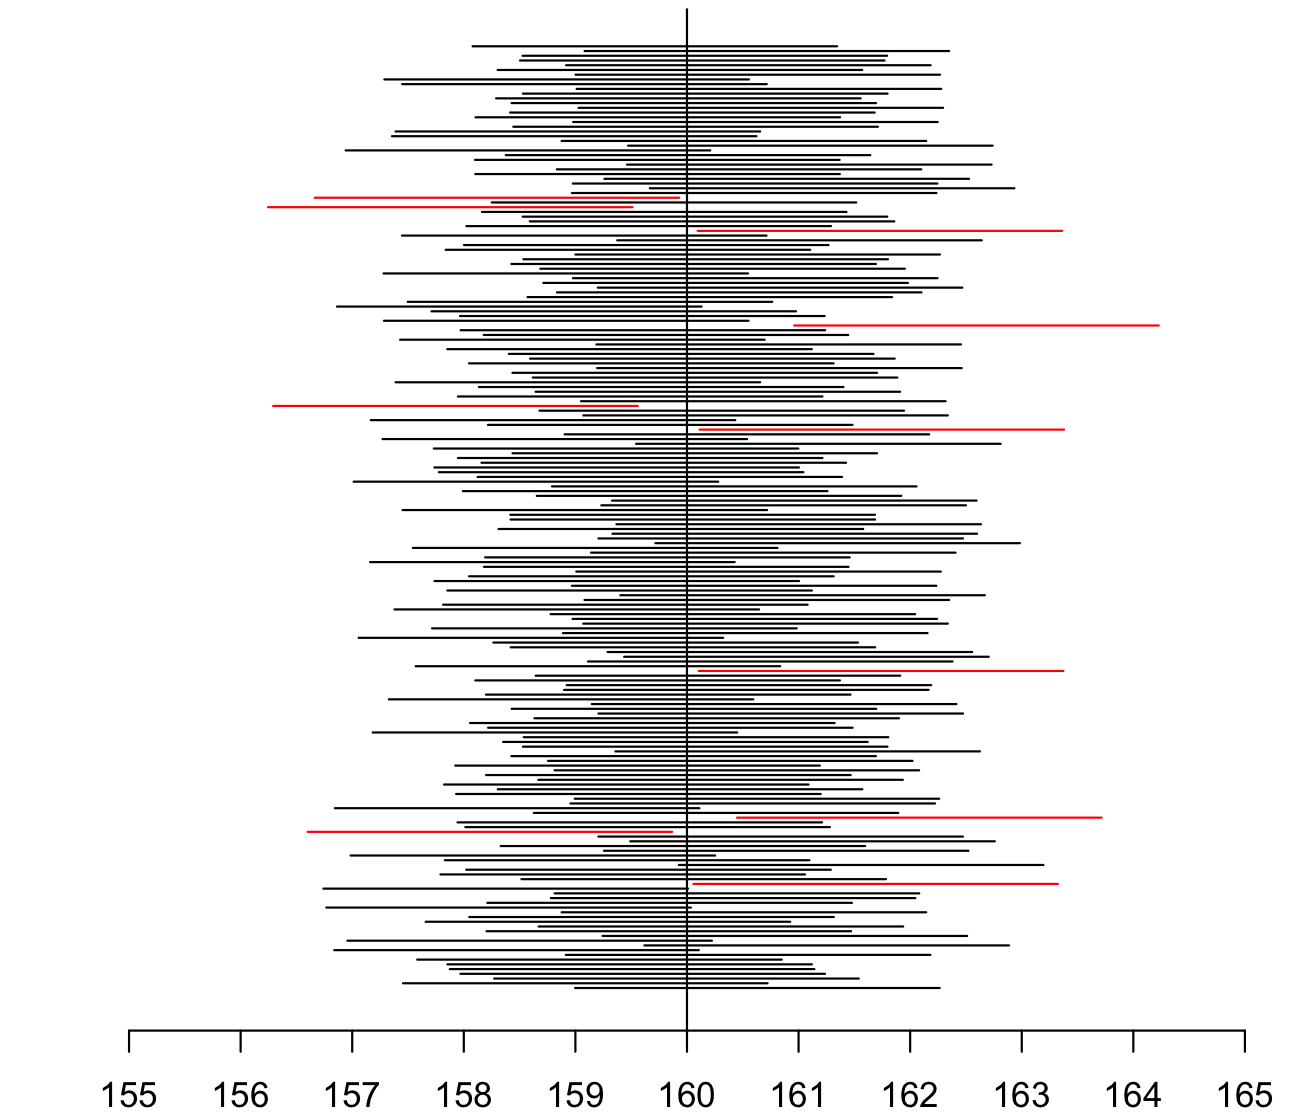
\includegraphics[width=0.7\textwidth]{figures/05-Confidence_interval/Confidence_interval.png}
        \caption{從 $\NN(160, 5^2)$ 抽出樣本數 36 的 200 組樣本,所得到的200個平均值 95\% 信賴區間}
        \label{fig:confidence_interval}
    \end{figure}
    
    注意到上述信賴區間性質的定義中,隨著每次抽樣,$\bar{X}$會有所變動,因此\textbf{整個區間會隨著抽樣而有不確定性}。這個「區間具有不確定性」的觀念可以衍生出兩個重點:
    \begin{itemize}
        \item 信賴區間的機率是針對「產生信賴區間的算法」而非觀察到的信賴區間數值:我們抽得一個樣本後,可以根據該樣本的觀察值算出一個區間(即圖 \ref{fig:confidence_interval}中的其中一條橫線)。但這個區間只是眾多可能的區間中被抽樣出來的一個,而信賴區間裡的 $95\%$ 是針對整體可能的區間作的機率性描述,而不是針對單一的區間觀察值。
        \item 參數雖未知但不具變動性,區間才有抽樣造成的變動性:前面我們在描述 $\PP\big(\mu \in \big(\bar{X}-z_{0.025}\cdot \frac{5}{6},  \bar{X} + z_{0.025}\cdot \frac{5}{6}\big)\big)$ 時,不用 $\mu$ 「落在」區間的機率,而是用區間「覆蓋」$\mu$ 的機率,即為強調 $\mu$ 本身不動,是區間在隨著抽樣而變動的概念。
    \end{itemize}
    前面我們用了一些實際數字來演示信賴區間的建構方法。利用符號來一般性地說明的話,假設母體來自於已知標準差為 $\sigma$ 的常態分佈,且 $\bar{X}$ 為樣本數 $n$ 的樣本算出的樣本平均,則母體平均值的 $(1-\alpha) \times 100\%$ 雙尾信賴區間可寫為
    \[\Big(\bar{X}-z_{\alpha/2}\frac{\sigma}{\sqrt{n}},  \bar{X} + z_{\alpha/2}\frac{\sigma}{\sqrt{n}}\Big)\]
    可以看到,這個雙尾區間以樣本平均 $\bar{X}$ 為中心,左右的寬度則各為 $z_{\alpha/2}\frac{\sigma}{\sqrt{n}}$。寬度取決於三個因子:
    \begin{itemize}
        \item 母體標準差 $\sigma$:母體的標準差越大,信賴區間的寬度越寬,意味著估計的不確定度越高。
        \item 樣本數 $n$:樣本數越大,信賴區間的寬度越窄,意味著估計越精準。
        \item 信賴區間的覆蓋率 $1-\alpha$:覆蓋率越高,$\alpha$越小,$z_{\alpha/2}$的值就越大,信賴區間的寬度就越寬。意即要提高覆蓋率,就要把信賴區間拉寬作為代價。
    \end{itemize}
    若我們有興趣的是單尾的信賴區間,則可以利用 $\PP(\ZZ > -z_{\alpha}) = \PP(\ZZ < z_{\alpha}) = 1-\alpha$ ,以相同的推導方式建立出下列右尾和左尾$(1-\alpha) \times 100\%$信賴區間:
    \[\Big(\bar{X}-z_{\alpha}\frac{\sigma}{\sqrt{n}},  \infty\Big), \;\;\Big(-\infty,  \bar{X} + z_{\alpha}\frac{\sigma}{\sqrt{n}}\Big)\]
    
    \begin{custom}{思考}
       在這個常態分布的例子中,如果要讓平均值信賴區間的覆蓋機率達到 100 \%,那麼寬度會變成多寬?
    \end{custom}

    \bigskip

    \begin{custom}{練習}
        假設已知 60 歲以上國人血清低密度脂蛋白的濃度標準差為 10 mg/dL,且呈現常態分布。現隨機選取 400 位 60 歲以上的志願者抽血,得到血清低密度脂蛋白的平均濃度為 93 mg/dL。請問 60 歲以上國人平均血清低密度脂蛋白濃度的 (1) 雙尾 95\% 信賴區間為何? (2) 右尾 90\% 信賴區間為何?
    \end{custom}

    \bigskip

    若母體並非來自常態分布,平均值信賴區間的建構較不直觀。然而,當樣本數夠大時,我們還有一個重要的法寶:中央極限定理!舉例來說,如果母體分布為機率參數為 $p$ 的白努利分布,那麼抽取樣本數為 $n$ 的樣本後,計算樣本中取值 1 的比例 $\hat{p}$ 相當於計算樣本平均值。根據中央極限定理:
    \[\hat{p} \xrightarrow{d} \NN\Big(p, \frac{p(1-p)}{n}\Big)\]
    所以利用類似常態分布的方法,我們可以構造以下關於 $p$ 的(近似) $(1-\alpha)\times 100\%$雙尾信賴區間
    \[\Big(\hat{p} - z_{\alpha/2} \sqrt{\frac{p(1-p)}{n}}, \hat{p} + z_{\alpha/2} \sqrt{\frac{p(1-p)}{n}}\Big)\]
    不過上面式子的問題是,根號中的 $p$ 仍是未知的參數,所以我們用 $p$ 最好的估計值 $\hat{p}$ 來取代 $p$,最終得到
    \[\Big(\hat{p} - z_{\alpha/2} \sqrt{\frac{\hat{p}(1-\hat{p})}{n}}, \hat{p} + z_{\alpha/2} \sqrt{\frac{\hat{p}(1-\hat{p})}{n}}\Big)\]
    這個公式也常被當成是比例信賴區間的通式。同樣地,右尾和左尾的(近似) $(1-\alpha)\times 100\%$單尾信賴區間為
    \[\Big(\hat{p} - z_{\alpha} \sqrt{\frac{\hat{p}(1-\hat{p})}{n}}, 1\Big), \;\; \Big(0, \hat{p} + z_{\alpha} \sqrt{\frac{\hat{p}(1-\hat{p})}{n}}\Big)\]
    此處左右尾的界線設定在 0 和 1,因為實際上的參數 $p$ 不可能超過 $[0,1]$ 的範圍。注意到這些近似信賴區間只有在 $n$ 夠大的時候,聲稱的 $(1-\alpha)\times 100\%$ 覆蓋率才會成立。一般而言,當 $np$ 及 $n(1-p)$ 均大於 $5$ 時,這個信賴區間的表現就已經很不錯。

    \bigskip
    
    \begin{custom}{練習}
        某大型醫療體系對員工進行血糖抽檢,隨機抽檢 160 人後發現,有 12 員工呈現空腹血糖過高的現象。請問該體系員工空腹血糖過高比率之 95\% 信賴區間為何?
    \end{custom}

    \bigskip

    \begin{custom}{練習}
        某民調公司希望藉由隨機電訪了解民眾對於 A 總統的支持度。若民調公司希望無論調查結果如何,最後建構出之支持度 95\% 雙尾信賴區間均不寬於上下 3\% (也就是總寬度不超過 6\%),那麼至少應收回多少有效電訪樣本?
    \end{custom}

    \bigskip

    前面我們針對常態分布的母體平均建立信賴區間時,作了一個不太常見的假設:母體標準差已知為。大部分的情況下,母體標準差都是未知的,因此雙尾信賴區間的公式就會多出一個未知數 $\sigma$。最直覺的解決辦法是直接參考比例信賴區間的做法,用樣本標準差帶入 $\sigma$,但這個方法在 $n$ 不夠大時,樣本標準差估計的準確度不佳,會造成整體的信賴區間覆蓋率不足。舉例來說,圖\ref{fig:confidence_t}中,假設母體和圖\ref{fig:confidence_interval}一樣服從 $\NN(160, 5^2)$,但是樣本數只有 9,且我們使用前述的雙尾 95\% 信賴區間公式並把 $\sigma$ 帶入樣本標準差,則 200 個平均值信賴區間中,有高達 18 個沒有覆蓋到正確值 160!

    \begin{figure}[htbp]
        \centering
        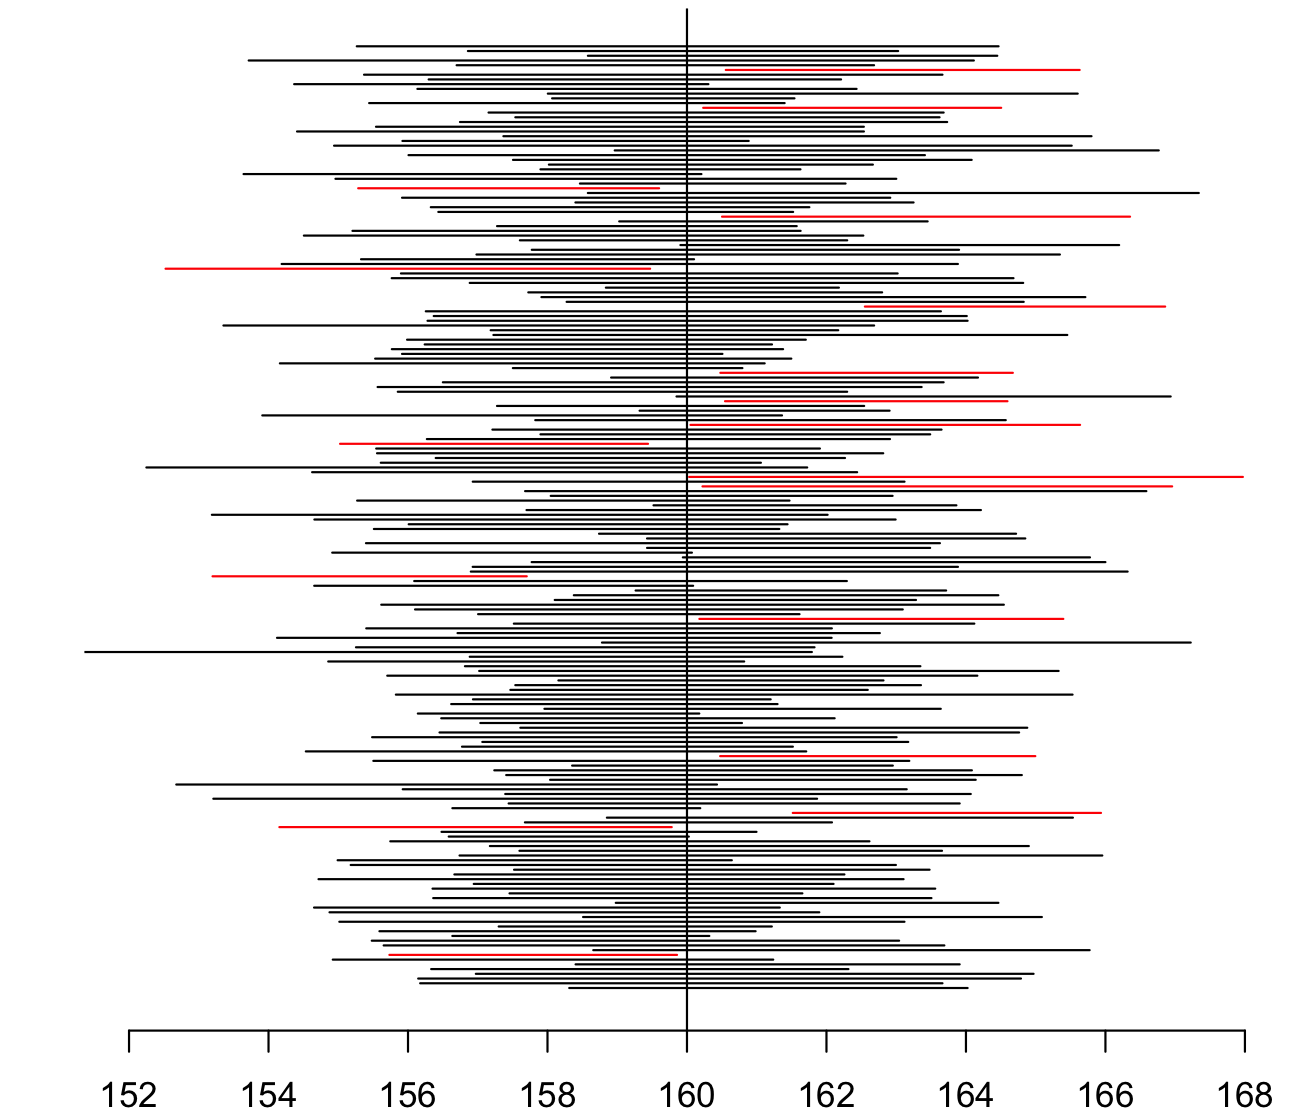
\includegraphics[width=0.7\textwidth]{figures/05-Confidence_interval/confidence_t.png}
        \caption{從 $\NN(160, 5^2)$ 抽出樣本數 9 的 200 組樣本所得的信賴區間(樣本標準差帶入母體標準差)}
        \label{fig:confidence_t}
    \end{figure}

    幸運的是,統計學家 William Gosset(1876—1937)在 1906 年初提出了一個新的分布,能夠幫助我們找出在這個情境中精確建構信賴區間的方法。Gosset 發現,若母體服從平均值為 $\mu$ 的常態分布,抽取樣本數為 $n$ 的樣本得到樣本平均 $\bar{X}$ 及樣本標準差 $s$,則
    \[\frac{\bar{X}-\mu}{s/\sqrt{n}} \sim t_{n-1}\]
    其中 $t_{n-1}$ 就是 Gosset 提出的 student $t$ 分布(這裡如果 $t$ 能夠大寫代表隨機變數的確比較不容易混淆,但是統計學界的習慣都寫小寫)。下標的 $n-1$ 是 $t$ 分布唯一的參數,被稱為\textit{自由度} (degrees of freedom)。這個自由度的由來可以看成是分母在計算樣本標準差時,使用的樣本數減去估計的參數個數,因此是 $n$ 個樣本減掉估計了一個樣本平均,總自由度為 $n-1$。$t$ 分布的機率密度函數如圖\ref{fig:student}所示。可以看到相對於標準常態分佈(黑色粗線) 而言,$t$ 分布的分布比較分散,雙尾比較厚重。但是隨著自由度 $\nu$ 上升,$t$ 分布的形狀會越來越接近標準常態分佈。事實上,當自由度 $\nu > 30$ 時,一般認為 $t$ 分布可以直接用標準常態分佈來近似。針對 $t$ 分布,我們也有 \href{https://en.wikipedia.org/wiki/Student%27s_t-distribution}{$t$分布表}可以查詢其曲線下面積。

    \begin{figure}[htbp]
        \centering
        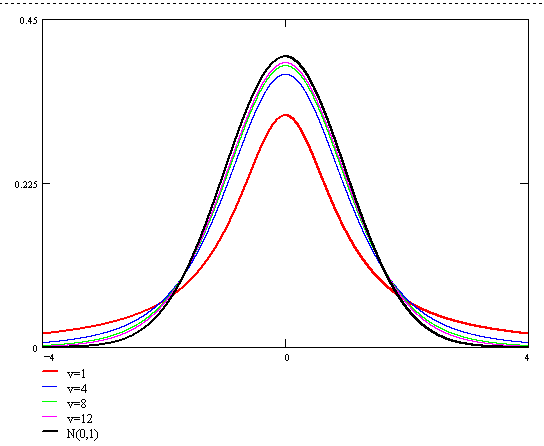
\includegraphics[trim={0 0 0 0.5cm},clip,width=0.7\textwidth]{figures/05-Confidence_interval/student.png}
        \caption{$t$分布的機率密度函數}
        \label{fig:student}
    \end{figure}

    回到我們建構信賴區間的目標,現在我們知道 $\frac{\bar{X}-\mu}{s/\sqrt{n}}$ 服從一個已知的 $t_{n-1}$ 分布,因此它又是一個樞紐量,我們可以參考前面的推導過程,先從以下的等式出發,建構出一個以 0 為中心左右對稱,且機率為 $(1-\alpha)\times 100\%$ 的區間:
     \[\PP(-t_{n-1, \alpha/2} < t_{n-1} < t_{n-1, \alpha/2}) = \alpha\]
    其中 $t_{\nu, p}$ 代表滿足 $\PP(t_{\nu} > t_{\nu, p}) = p$的數值,可以用查表得到。根據前面的分布,我們可以推出:
    \begin{align*}
        \PP\Big(-t_{n-1, \alpha/2} < \frac{\bar{X} - \mu}{s/\sqrt{n}} < t_{n-1, \alpha/2})\Big) &= \alpha\\
        \PP\Big(-t_{n-1, \alpha/2}\frac{s}{\sqrt{n}} < \bar{X} - \mu < t_{n-1, \alpha/2}\frac{s}{\sqrt{n}}\Big) &= \alpha\\
        \PP\Big(\bar{X}-t_{n-1, \alpha/2}\frac{s}{\sqrt{n}}< \mu < \bar{X} + t_{n-1, \alpha/2}\frac{s}{\sqrt{n}}\Big) &= \alpha\\
        \PP\Big(\mu \in \Big(\bar{X}-t_{n-1, \alpha/2}\frac{s}{\sqrt{n}},  \bar{X} + t_{n-1, \alpha/2}\frac{s}{\sqrt{n}}\Big)\Big) &= \alpha
    \end{align*}
    因此,母體為常態分布下的母體平均值 $(1-\alpha)\times 100\%$ 信賴區間可以寫為
    \[\Big(\bar{X}-t_{n-1, \alpha/2}\frac{s}{\sqrt{n}},  \bar{X} + t_{n-1, \alpha/2}\frac{s}{\sqrt{n}}\Big)\]
    可以看到,用 $t$ 分布建構的信賴區間和常態分布建構的信賴區間,基本上只差在臨界值改成查 $t_{n-1}$ 的表、以及標準差由母體標準差改為樣本標準差。前面我們提到 $t$ 分布都比標準常態分佈來得寬,所以 $t_{n-1, \alpha/2}$ 會比 $z_{\alpha/2}$ 來得大,也就是 $t$ 分布建構的信賴區間比常態分布建構的信賴區間來得寬。
    
    用類似的推導也可以得到右尾和左尾的 $(1-\alpha)\times 100\%$ 信賴區間分別可以寫為
    \[\Big(-\infty,  \bar{X} + t_{n-1, \alpha}\frac{s}{\sqrt{n}}\Big), \;\;\Big(\bar{X}-t_{n-1, \alpha}\frac{s}{\sqrt{n}},  \infty\Big)\]

    \bigskip

    \begin{custom}{練習}
        假設已知 60 歲以上國人血清低密度脂蛋白的濃度呈現常態分布。現隨機選取 16 位 60 歲以上的志願者抽血,得到血清低密度脂蛋白的平均濃度為 93 mg/dL,樣本標準差為 9 mg/dL。請問 60 歲以上國人平均血清低密度脂蛋白濃度的 (1) 雙尾 95\% 信賴區間為何? (2) 右尾 90\% 信賴區間為何?
    \end{custom}
    
    \begin{docexam}{(107-1醫學(二))}
        為了探討某社區之吸菸盛行狀況,由此社區隨機選取100位居民,發現其中30位居民具有吸菸習慣。在 5\% 的誤差水準下,此社區吸菸率的 95\% 信賴區間之上限值為何?
    \end{docexam} 
    
    \begin{docexam}{(103-1醫學(一))}
        對 100 名國小六年級學童量測體重,發現樣本平均值為 35 公斤,母群體平均值的 95\% 信賴區間為 33 公斤至 37 公斤。下列敘述何者正確?

        (A) 母群體平均值為 35 公斤

        (B) 該研究 100 名國小學童中,95 名的體重介在 33 至 37 公斤之間

        (C) 該樣本學童的體重標準差約 10 公斤

        (D) 若計算母群體平均值的 90 \% 信賴區間,其範圍會大於 95\% 信賴區間
    \end{docexam}
\chapter{推論統計:假說檢定}

    推論統計的目的是了解背後母群體的特性,或更精確地來說,背後母群體的參數取值狀況。例如在民意調查中,我們感興趣的母體參數是全民政策支持率 $p$,而推論統計希望可以藉由有限的抽樣樣本來了解 $p$ 的取值。推論統計的方法主要可以分成兩大分支:估計以及假說檢定。估計採取的策略較為直接,希望可以從樣本計算出一個估計值(點估計)或估計區間(區間估計),來描述 $p$ 的可能取值。假說檢定採取的則是科學中假說-預測-證偽的典範,首先提出假說,並根據假說預測觀察資料應有的特徵,而後實際檢視資料是否\textbf{不符}該特徵而將假說\textbf{證偽}。本章將探討如何將上述流程具象化為統計檢定的步驟,其中會大量用到條件機率以及抽樣分布的概念,希望讀者能夠融會貫通。
    
    \begin{introduction}[第 \thechapter 章學習目標]
        \item 建構假說檢定的基本架構
        \item 虛無假說、對立假說、虛無分布及顯著水準的意義
        \item 了解如何解釋 $p$ 值
        \item 常見情境的母體平均單樣本檢定
        \item 信賴區間與檢定的關係
        \item 檢定的型一錯誤率、型二錯誤率、檢定力與樣本數計算
    \end{introduction}

\section{假說檢定的基本架構}

    在進入假說檢定的架構前,我們先考慮以下的情境:假設某 A 同學宣稱他有猜拳的天賦,贏拳的機率高於一般認為的 1/3。你不相信並想要挑戰他。於是,你跟他猜了五次拳,結果他贏了四次。這時候你想著,如果他猜拳能力只是一般的 1/3,那麽猜五次裡面贏四次以上的機率是(根據我們學到的二項分布機率質量函數)
    \[\binom{5}{4} \cdot \Big(\frac{1}{3}\Big)^4 \cdot \frac{2}{3} + \binom{5}{5} \cdot \Big(\frac{1}{3}\Big)^5 \approx 0.0453\]
    也就是說,如果他只是一般的猜拳者,那麼他贏得這麼徹底的機率只有約 $4.5 \%$。你覺得這樣的機率太低了,不太可能發生。因此,你認為 A 同學的確有一些猜拳的技術,讓他的猜拳贏拳機率比 1/3 還要高。

    上述的流程雖然十分簡單,但已經蘊含了假說檢定的基本架構。首先,我們需要有一個想\textbf{證偽}的命題,並把這個命題量化成為一個假說。這個假說建立的目的是要被證偽,因此被稱為\textit{虛無假說} (null hypothesis),符號上通常記為 $H_0$。上述的情境中,我們想要證偽的命題是「A 同學的猜拳能力等同一般人」,量化後的虛無假說即為「A 同學猜拳贏拳的機率 $p = 1/3$」。有了虛無假說後,我們還需要建立虛無假說的對立面,也就是將虛無假說證偽後希望得到的結論。這個對立的假說被稱為\textit{對立假說} (alternative hypothesis),符號上通常記為 $H_1$ 或 $H_a$。上述情境中,我們希望證偽虛無假說後,能夠認定 A 同學真的有猜拳的天賦,因此對立假說是「A 同學猜拳贏拳的機率 $p > 1/3$」(注意到對立假說不一定要是虛無假說的補集)。我們通常會將這兩個假說並陳如下(令 $p$ 為 A 同學猜拳贏拳的機率):
    \begin{align*}
        H_0: \;&p = 1/3\\
        H_1: \;&p > 1/3
    \end{align*}
    訂好假說後,我們要判斷資料是否\textbf{不符合}虛無假說下的情境,以決定是否能證偽虛無假說。為了方便判斷,我們會利用資料計算出一個\textit{測驗統計量},這個測驗統計量通常會儘量滿足兩個特點:(1) 我們知道該統計量在虛無假說下的抽樣分布,這個分布被稱為虛無分布 (null distribution) (2) 當對立假說成立時,該統計量的取值落在虛無分布較極端的位置,例如偏大、偏小、或是在分布的兩端。需要這兩點的原因在於,我們希望算出測驗統計量時,可以用方向來判斷統計量是否偏離虛無假說並偏向對立假說,並且能用虛無分布來量化該統計量有多極端。在上述的例子中,我們的測驗統計量是猜拳五次後 A 同學贏的總次數,我們簡單記為 $T$。我們知道 $T$ 在虛無假說下服從一個次數參數為 5、機率參數為 1/3 的二項分布。此分佈即虛無分布,如圖 \ref{fig:null_dist_binom}。而且我們還知道,當對立假說成立時,$T$ 的取值應該會偏大。因此,$T$ 符合我們對於測驗統計量的要求。

    \begin{figure}[htbp]
        \centering
        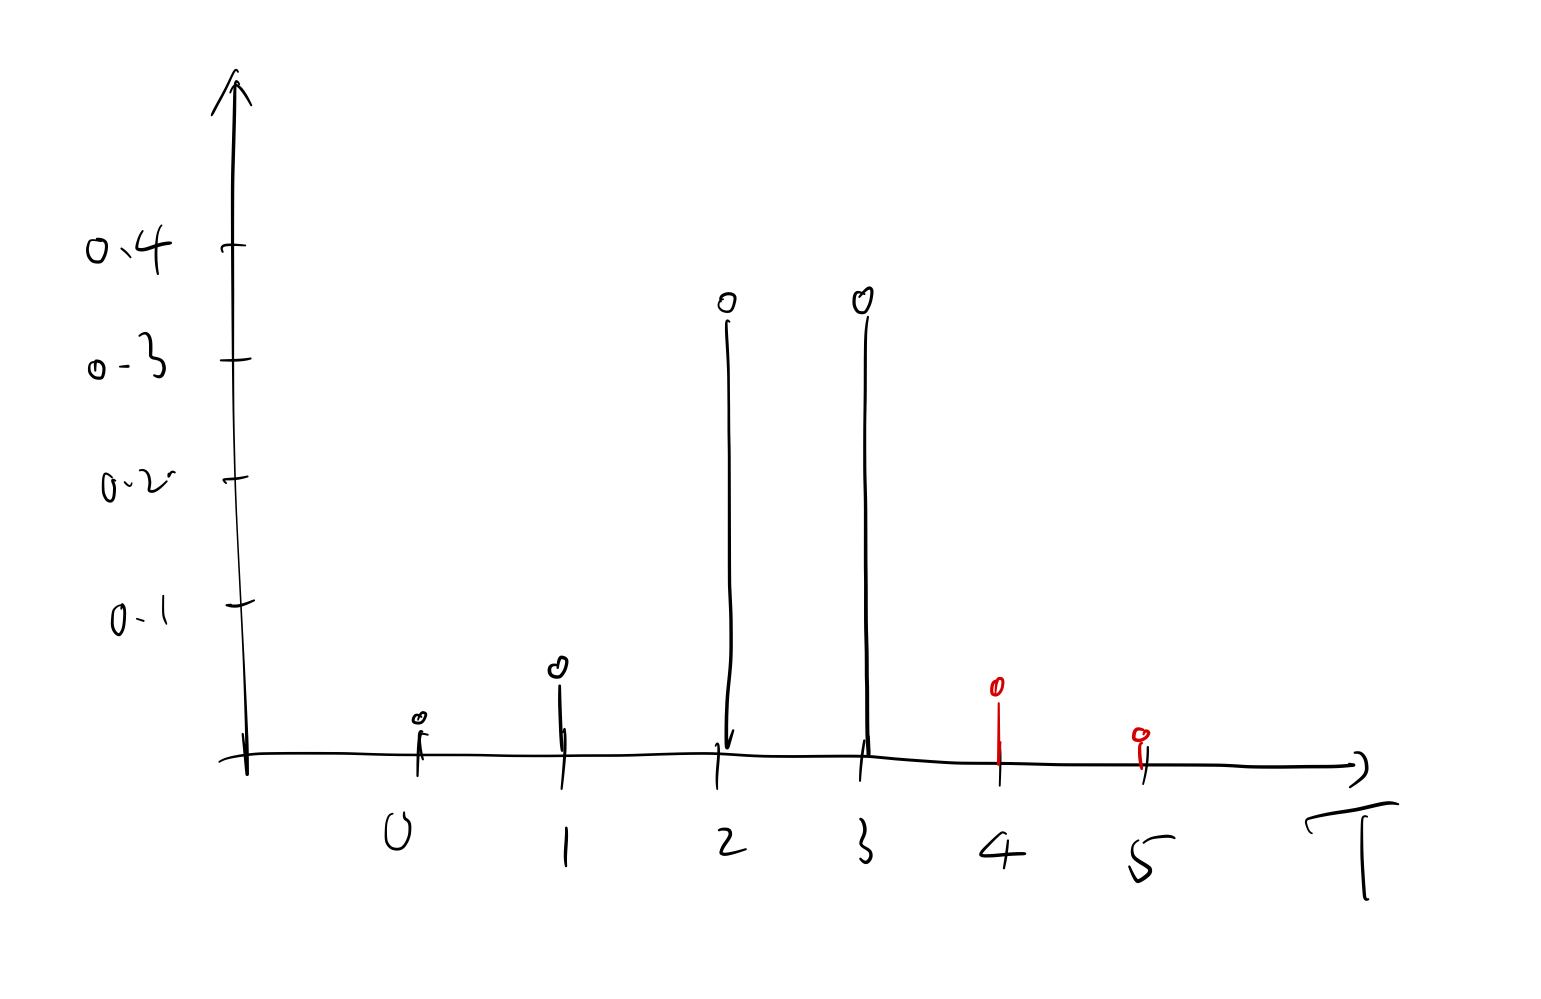
\includegraphics[width=0.7\textwidth]{figures/06-Hypothesis_testing/null_dist_binom.jpeg}
        \caption{猜拳實驗假說檢定的虛無分佈}
        \label{fig:null_dist_binom}
    \end{figure}
 
    接下來,我們要用虛無分布來量化我們觀察到的 $T=4$ 是否足夠極端。我們量化的方法是計算「在虛無分布下,$T$ 的取值和觀察值一樣極端,或比觀察值還要極端的機率」,其中極端的定義是接近對立假說的取值。例如上述情況中,我們知道 $T$ 取值越大,代表贏拳次數越多,也就越接近我們的對立假說。因此,我們要計算「在虛無分布下,$T$ 的取值大於或等於 $4$ 的機率」,也就是圖 \ref{fig:null_dist_binom}中兩個紅色的機率相加,我們之前算出是 0.0453。這個機率我們稱為檢定的 $p$\textit{值} ($p$-value)。該值越小,代表測驗統計量處於越極端的的位置,也就隱含著虛無假設越不可能成立。

    在上述的例子中,我們認為 $p$ 值 0.0453「夠小」,足以證偽虛無假設而接受對立假設 $p > 1/3$,也就是 A 同學有優於常人的猜拳能力。然而,有些人可能認為 0.0453 不夠小,仍然無法排除是 A 同學只是運氣好贏了四次。因此,我們需要訂定一個判準來決定怎麼樣子的 $p$ 值叫做「夠小」。這個判準通常被稱為\textit{顯著水準} (significance level),符號寫作 $\alpha$。當 $p \le \alpha$ 時,我們就認為 $p$ 值夠小,並稱檢定\textit{顯著} (significant),可以拒絕虛無假說並接受對立假設。這種檢定的方法我們稱為 \textbf{$p$ 值法}。舉例來說,上述的例子我們可以設定顯著水準為 0.05,並注意到 $p = 0.0453 \le 0.05$,因此「在顯著水準 0.05 下,我們拒絕虛無假說,並得出 A 同學有\textit{統計上顯著} (statistically significant) 優於常人的猜拳能力」。但若設定顯著水準為 0.01,因為 $p = 0.0435 > 0.01$,只能說「在顯著水準 0.01 下,我們\textbf{無法拒絕}虛無假說,因此\textbf{沒有足夠證據證明} A 同學的猜拳能力優於常人」。

    從圖 \ref{fig:null_dist_binom} 可以看出,如果我們設定 $\alpha = 0.05$,由於我們只有在 $p$ 值小於 $0.05$ 時才拒絕虛無假說,因此只有 $T \ge 4$ 時才會拒絕虛無假說($\PP(T \ge 3 | H_0) = 0.5 \ge 0.05$)。這個 $T \ge 4$ 也被稱為檢定的\textit{拒絕域} (rejection region),而其邊界 $T=4$ 則是檢定的\textit{臨界值} (critical value)。如果我們可以先找到拒絕域 $T \ge 4$,就可以在不用算出 $p$ 值的情況下,僅憑檢定統計量 $T$ 的觀察值逕行決定是否拒絕虛無假說。這種檢定方法我們稱為\textbf{拒絕域法}。
    
    拒絕域的建構方法如下:首先我們需要根據虛無假說及對立假說的相對關係決定拒絕域的型態。例如上述例子中,我們知道 $T$ 越大,證據越偏向對立假說,因此拒絕域的型態應該型如 $T \ge c$,其中 $c$ 是待定的常數。然後,我們需要找到符合 $\PP(T \ge c | H_0) \le \alpha$ 的條件下,讓拒絕域最大化的 $c$。其中 $\PP(T \ge c | H_0)$ 代表「在虛無假說正確下拒絕虛無假說」的機率,也就是「冤枉了虛無假說」的機率。這種「冤枉虛無假說」事件也被稱為犯下\textit{型一錯誤} (type I error)。換言之,我們希望在控制型一錯誤率不高於顯著水準的情況下,盡可能地擴大拒絕域。在上述的例子中,若將顯著水準 $\alpha$ 設定為 0.05,則 $c$ 最小的可行取值為 $4$,因為 $\PP(T \ge 4 | H_0) = 0.0453 \le 0.05, \PP(T \ge 3 | H_0) = 0.5 > 0.05$。因此,顯著水準 0.05 下的拒絕域為 $T \ge 4$,臨界值為 $4$。

    從前面的討論可以看到,統計檢定顯著與否有一大部分取決於顯著水準 $\alpha$。為了避免做檢定時看到檢定統計量觀察值才移動顯著水準,進而操弄檢定的顯著性,一般我們會在進行檢定前就設定好顯著水準。在生醫統計中最常使用的顯著水準為 0.05,但在一些特別的檢定也可能設定為 0.1 或 0.01。事實上,0.05 的設定完全沒有科學根據,僅是根據 Ronald Fisher 在一篇文章寫到「... Personally, the writer prefers to set a low standard of significance at the 5 per cent. point, ...」,後人效仿後漸漸成為約定俗成。

    最後,我們把統計檢定的步驟作成如圖 \ref{fig:hypothesis_flowchart} 的流程圖。

    \bigskip

    \begin{custom}{思考}
       如果把顯著水準提高,拒絕域應該會變寬或是變窄?
    \end{custom}

    \begin{figure}
        \begin{center}
            \begin{tikzpicture}[node distance=1.5cm]
                \node (one) [rnd] {1. 寫出欲證偽的命題,以及與該命題對立、證偽後欲接受的命題};
                \node (two) [rnd, below of = one] {2. 將命題量化為虛無假說與對立假說};
                \node (three) [rnd, below of = two] {3. 訂定顯著水準 $\alpha$};
                \node (four) [rnd, below of = three] {4. 選定檢定統計量 $T$ 並計算數值};
                \node (five) [below of = four, yshift = -1cm] {};
                \node (six) [below of = five] {};
                \node (seven) [below of = six, yshift = -1cm] {};
                \node (fiveone) [rnd, left of = five, xshift = -2cm] {5-1. 根據 $\alpha$ 計算臨界值與拒絕域};
                \node (sixone) [rnd, below of = fiveone] {6-1. 判定 $T$ 是否落在拒絕域};
                \node (fivetwo) [rnd, right of = five, xshift = 2cm] {5-2. 計算 $p$ 值};
                \node (sixtwo) [rnd, below of = fivetwo] {6-2. 判定是否 $p \le \alpha$};
                \node (sevenr) [rnd, below of = sixone, yshift = -1cm] {7a. 拒絕虛無假說,接受對立假說};
                \node (sevena) [rnd, below of = sixtwo, yshift = -1cm] {7b. 無法拒絕虛無假說};
                \node (eight) [rnd, below of = seven] {8. 撰寫結論};
                \draw [arrow] (one) -- (two);
                \draw [arrow] (two) -- (three);
                \draw [arrow] (three) -- (four);
                \draw [arrow] (four) -- node[anchor=east] {拒絕域法}(fiveone);
                \draw [arrow] (four) -- node[anchor=west] {$p$值法}(fivetwo);
                \draw [arrow] (fiveone) -- (sixone);
                \draw [arrow] (fivetwo) -- (sixtwo);
                \draw [arrow] (sixone) -- node[anchor=east] {是} (sevenr);
                \draw [arrow] (sixtwo) -- node[anchor=south east] {否} (sevenr);
                \draw [arrow] (sixone) -- node[anchor=south west] {是} (sevena);
                \draw [arrow] (sixtwo) -- node[anchor=west] {否} (sevena);
                \draw [arrow] (sevenr) -- (eight);
                \draw [arrow] (sevena) -- (eight);
            \end{tikzpicture}
        \end{center}
        \caption{假說檢定流程圖}
        \label{fig:hypothesis_flowchart}
    \end{figure}

\section{母體平均的單樣本檢定:母體為常態分布且變異數已知}
    有了上一節的框架後,我們可以來看幾個情境下,針對母體平均的統計檢定。假設已知母體為常態分布且變異數已知為 $\sigma^2$,抽取樣本數為 $n$ 的樣本並得到樣本平均為 $\bar{X}$。我們分成三種情況討論(母體平均參數以 $\mu$ 表示):

    \noindent\underline{\textbf{右尾檢定}}

    若假說形如 $H_0: \; \mu = \mu_0 \; ; \; H_1: \; \mu > \mu_0$,則在虛無假說下,根據樣本平均的性質:
    \[\bar{X} \sim \NN\Big(\mu_0, \frac{\sigma^2}{n}\Big)\]
    因此我們可以把 $\bar{X}$ 作 $z$ 轉換當成檢定統計量,其虛無分布為標準常態分佈:
    \[Z = \frac{\bar{X}-\mu_0}{\sigma/\sqrt{n}} \sim \ZZ\]
    設定顯著水準為 $\alpha$ 的情況下,我們可以用 $p$ 值法或拒絕域法來建構檢定:

    \noindent \underline{$p$ 值法}:當對立假說為真時,$\bar{X}$ 的期望值 $\mu$ 會比 $\mu_0$ 來得大,因此 $Z$ 偏大的方向是比較「極端」的方向。根據 $p$ 值的定義可以寫出
    \[p = \PP(\ZZ \ge Z)\]
    即對應到圖\ref{fig:one_sample_z}左圖紅色的面積。此時若 $p \le \alpha$ 則拒絕虛無假說、接受對立假說;反之則無法拒絕虛無假說。
    
    \noindent \underline{拒絕域法}:因為 $Z$ 值偏大的方向是傾向對立假說,所以拒絕域應該形如 $Z \ge c$。此時我們希望控制型一錯誤率在 $\alpha$ 以內,因此需要
    \[\PP(Z \ge c|H_0) \le \alpha\]
    根據 $Z$ 的虛無分布,上述等價於
    \[\PP(\ZZ \ge c) \le \alpha\]
    滿足這個不等式最小的 $c$ 即為 $z_\alpha$(因為 $\PP(\ZZ \ge z_\alpha) = \alpha$),因此本檢定的拒絕區為 $Z \ge z_\alpha$,統計量臨界值為 $z_\alpha$,即對應到圖\ref{fig:one_sample_z}右圖紅色的切點,其中紅色面積為$\alpha$。可以看到拒絕區具有右邊的尾巴,所以這組虛無假說對應的檢定又稱為右尾檢定。若檢定統計量落在拒絕區,則拒絕虛無假說、接受對立假說;反之則無法拒絕虛無假說。

    \noindent\underline{\textbf{左尾檢定}}

    若假說形如 $H_0: \; \mu = \mu_0 \; ; \; H_1: \; \mu < \mu_0$,則檢定統計量和檢定統計量的虛無分佈均和右尾檢定相同,差別僅在於 $p$ 值法和拒絕域法的定義方向:

    \noindent \underline{$p$ 值法}:當對立假說為真時,$\bar{X}$ 的期望值 $\mu$ 會比 $\mu_0$ 來得小,因此 $Z$ 偏小的方向是比較「極端」的方向。根據 $p$ 值的定義可以寫出
    \[p = \PP(\ZZ \le Z)\]
    即對應到圖\ref{fig:one_sample_z}左圖黑色的面積。此時若 $p \le \alpha$ 則拒絕虛無假說、接受對立假說;反之則無法拒絕虛無假說。
    
    \noindent \underline{拒絕域法}:因為 $Z$ 值偏小的方向是傾向對立假說,所以拒絕域應該形如 $Z \le c$。經由相似的計算可得到拒絕區為 $Z \le -z_\alpha$,統計量臨界值為 $-z_\alpha$,即對應到圖\ref{fig:one_sample_z}右圖黑色的切點,其中黑色面積為$\alpha$。此拒絕區具有左邊的尾巴,所以這組虛無假說對應的檢定又稱為左尾檢定。若檢定統計量落在拒絕區,則拒絕虛無假說、接受對立假說;反之則無法拒絕虛無假說。

    \noindent\underline{\textbf{雙尾檢定}}

    若假說形如 $H_0: \; \mu = \mu_0 \; ; \; H_1: \; \mu \ne \mu_0$,則檢定統計量和檢定統計量的虛無分佈仍和右尾檢定相同,但 $p$ 值法和拒絕域法的定義方向則和前面兩個情境均不同。

    \noindent \underline{$p$ 值法}:當對立假說為真時,$\bar{X}$ 的期望值 $\mu$ 會往兩側遠離 $\mu_0$,因此 $Z$ 不論偏大或偏小都是「極端」的方向。且因為 $Z$ 的虛無分布期望值為零,$Z$ 和 $-Z$ 的極端程度是一樣的。如圖\ref{fig:one_sample_z}左圖所示。所以根據 $p$ 值的定義可以寫出
    \[p = \PP((\ZZ \ge |Z|)\cup(\ZZ \le -|Z|)) = 2\PP(\ZZ \ge |Z|)\]
    即對應到圖\ref{fig:one_sample_z}左圖藍色的面積。此時若 $p \le \alpha$ 則拒絕虛無假說、接受對立假說;反之則無法拒絕虛無假說。
    
    \noindent \underline{拒絕域法}:因為 $Z$ 值不論偏大或偏小均是傾向對立假說,而且 $Z$ 的虛無分布期望值為零,所以拒絕域應該形如 $(Z \ge c)\cup(Z \le -c)$,或可寫為$|Z| \ge c$。此時我們希望控制型一錯誤率在 $\alpha$ 以內,因此需要
    \[\PP(|Z| \ge c|H_0) \le \alpha\]
    根據 $Z$ 的虛無分布,上述等價於
    \[\PP(|\ZZ| \ge c) \le \alpha\]
    \[\PP(\ZZ \ge c) \le \alpha/2\]
    滿足這個不等式最小的 $c$ 即為 $z_{\alpha/2}$,因此本檢定的拒絕區為 $|Z| \ge z_{\alpha/2}$,統計量臨界值為 $\pm z_{\alpha/2}$,即對應到圖\ref{fig:one_sample_z}右圖藍色的切點,其中兩側藍色面積各為$\alpha/2$。此拒絕區兩邊均有尾巴,所以這組虛無假說對應的檢定又稱為雙尾檢定。若檢定統計量落在拒絕區,則拒絕虛無假說、接受對立假說;反之則無法拒絕虛無假說。

    \begin{figure}[htbp]
        \centering
        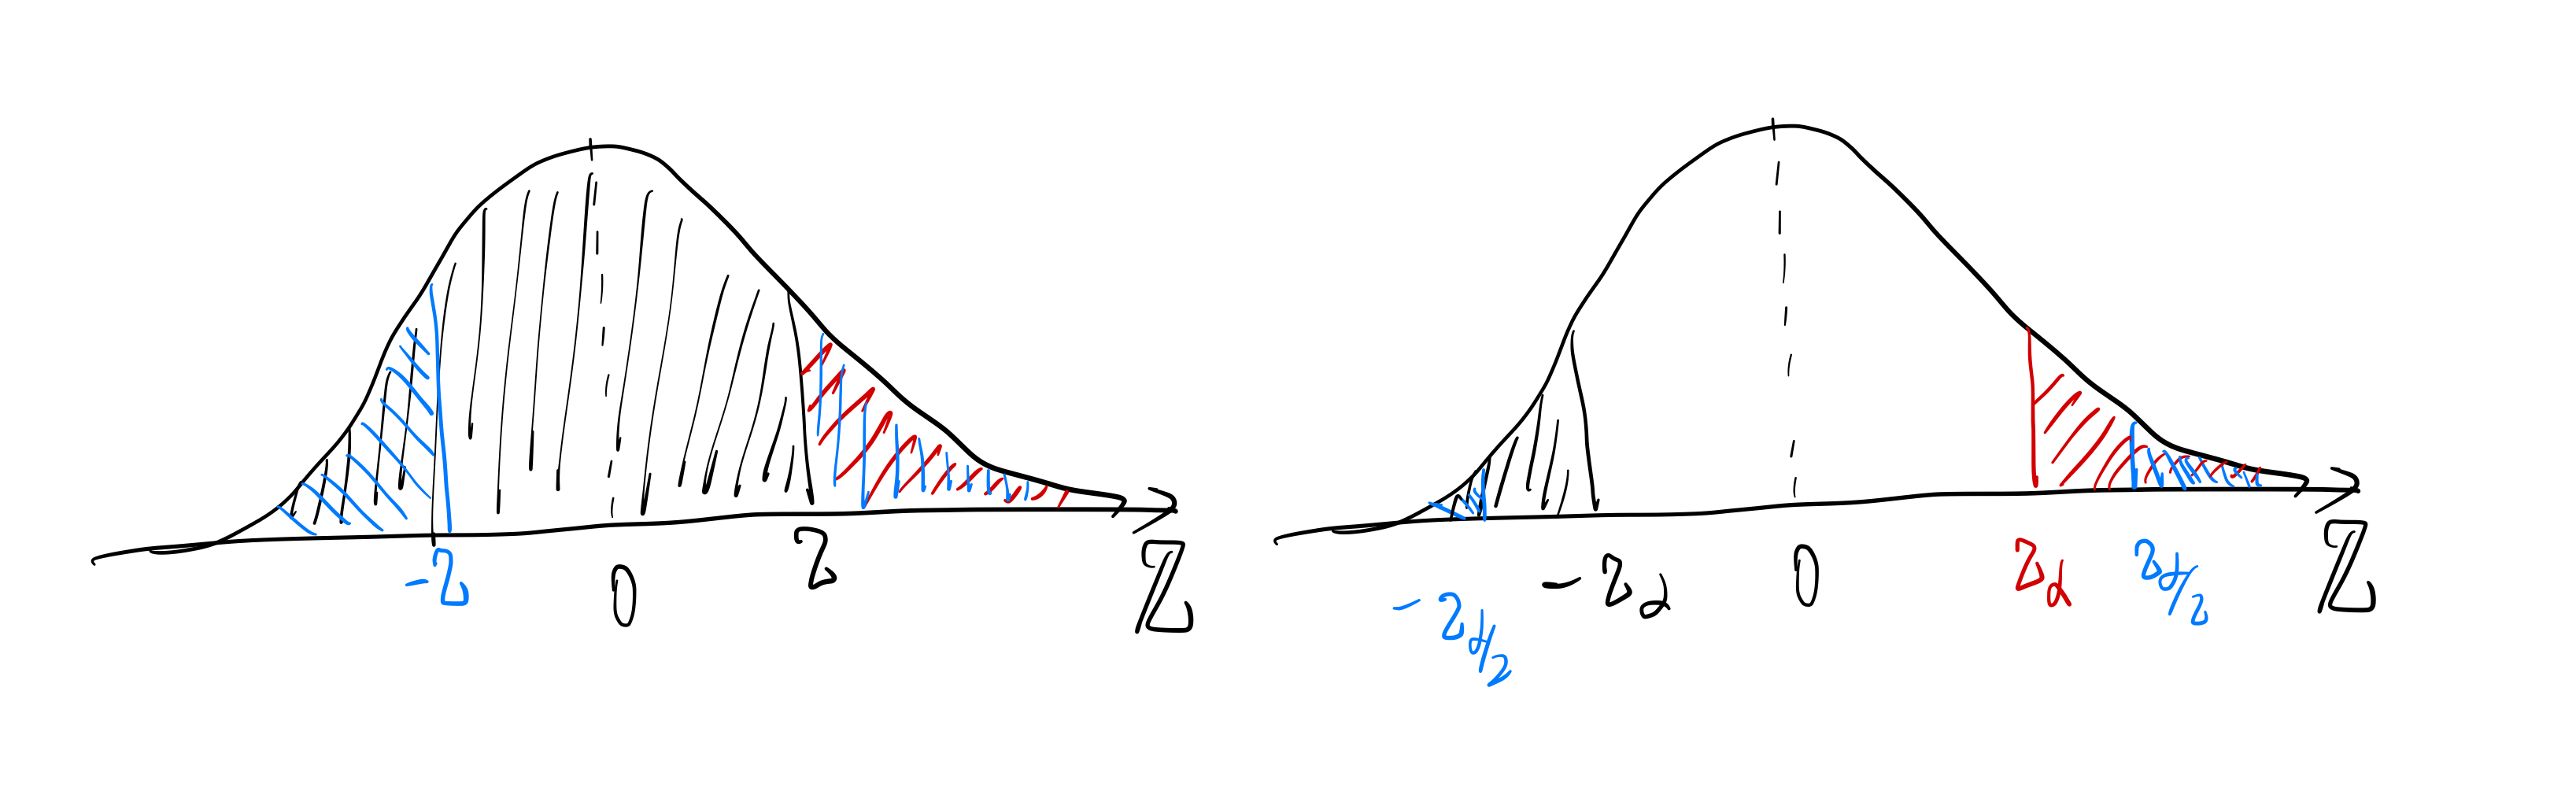
\includegraphics[width=\textwidth]{figures/06-Hypothesis_testing/one_sample_z.jpeg}
        \caption{母體為常態分布且變異數已知的母體平均檢定演示}
        \label{fig:one_sample_z}
    \end{figure}

    以下我們用表 \ref{tab:one_sample_z} 來整理母體為常態分布且變異數已知的母體平均檢定。由於此檢定只使用了一組樣本、是用 $Z$ 檢定統計量來建構、且統計量的虛無分布為標準常態分布($\ZZ$),因此此檢定亦稱為\textit{單樣本 Z 檢定} (One-sample Z test)。

    \begin{table}[htbp]
        \begin{center}
            \begin{tabular}{ccccc}
                \toprule
                虛無假說($H_0$) & 對立假說($H_1$) & 檢定統計量 & $p$ 值 & 拒絕區\\
                \hline
                \multirow{3}{*}{$\mu = \mu_0$} & $\mu > \mu_0$ & \multirow{3}{*}{$Z = \frac{\bar{X}-\mu_0}{\sigma/\sqrt{n}}$} & $\PP(\ZZ \ge Z)$ & $Z \ge z_{\alpha}$\\
                & $\mu < \mu_0$ & &$\PP(\ZZ \le Z)$&$Z \le -z_{\alpha}$\\
                & $\mu \ne \mu_0$ & &$2\times\PP(\ZZ \ge |Z|)$&$|Z| \ge z_{\alpha/2}$\\
                \bottomrule
            \end{tabular}
            \caption{母體為常態分布且變異數已知的母體平均檢定(單樣本 Z 檢定)\label{tab:one_sample_z}}
        \end{center}
    \end{table}
    
\section{母體平均的單樣本檢定:母體為常態分布且變異數未知}

    上一節我們假設了母體為常態分布且變異數已知,因此可以將樣本平均 $\bar{X}$ 進行 $z$ 轉換作為檢定統計量。然而,如果變異數未知,我們就無法直接作 $z$ 轉換了。幸運地是,在上一章我們提到的 $t$ 分布在這裡可以再度派上用場。假設已知母體為常態分布但變異數未知為,抽取樣本數為 $n$ 的樣本並得到樣本平均為 $\bar{X}$、樣本變異數為 $s^2$。我們仍然分成三種情況討論(母體平均參數以 $\mu$ 表示):

    \noindent\underline{\textbf{右尾檢定}}

    若假說形如 $H_0: \; \mu = \mu_0 \; ; \; H_1: \; \mu > \mu_0$,則在虛無假說下,根據$t$分布的定義:
    \[t = \frac{\bar{X}-\mu_0}{s/\sqrt{n}} \sim t_{n-1}\]
    設定顯著水準為 $\alpha$ 的情況下,我們用 $p$ 值法或拒絕域法來建構檢定:

    \noindent \underline{$p$ 值法}:當對立假說為真時,$\bar{X}$ 的期望值 $\mu$ 會比 $\mu_0$ 來得大,因此 $t$ 偏大的方向是比較「極端」的方向。根據 $p$ 值的定義可以寫出
    \[p = \PP(t_{n-1} \ge t)\]
    此時若 $p \le \alpha$ 則拒絕虛無假說、接受對立假說;反之則無法拒絕虛無假說。
    
    \noindent \underline{拒絕域法}:因為 $t$ 值偏大的方向是傾向對立假說,所以拒絕域應該形如 $t \ge c$。此時我們希望控制型一錯誤率在 $\alpha$ 以內,因此需要
    \[\PP(t \ge c|H_0) \le \alpha\]
    根據 $t$ 的虛無分布,上述等價於
    \[\PP(t_{n-1} \ge c) \le \alpha\]
    滿足這個不等式最小的 $c$ 為 $t_{n-1,\alpha}$(因為 $\PP(t_{n-1} \ge t_{n-1,\alpha}) = \alpha$),因此本檢定的拒絕區為 $t \ge t_{n-1,\alpha}$,統計量臨界值為 $t_{n-1,\alpha}$。若檢定統計量落在拒絕區,則拒絕虛無假說、接受對立假說;反之則無法拒絕虛無假說。

    \noindent\underline{\textbf{左尾檢定}}

    若假說形如 $H_0: \; \mu = \mu_0 \; ; \; H_1: \; \mu < \mu_0$,則檢定統計量和檢定統計量的虛無分佈均和右尾檢定相同,差別僅在於 $p$ 值法和拒絕域法的定義方向:

    \noindent \underline{$p$ 值法}:當對立假說為真時,$\bar{X}$ 的期望值 $\mu$ 會比 $\mu_0$ 來得小,因此 $t$ 偏小的方向是比較「極端」的方向。根據 $p$ 值的定義可以寫出
    \[p = \PP(t_{n-1} \le t)\]
    此時若 $p \le \alpha$ 則拒絕虛無假說、接受對立假說;反之則無法拒絕虛無假說。
    
    \noindent \underline{拒絕域法}:因為 $t$ 值偏小的方向是傾向對立假說,所以拒絕域應該形如 $t \le c$。經由相似的計算可得到拒絕區為 $t \le -t_{n-1,\alpha}$,統計量臨界值為 $-t_{n-1,\alpha}$。若檢定統計量落在拒絕區,則拒絕虛無假說、接受對立假說;反之則無法拒絕虛無假說。

    \noindent\underline{\textbf{雙尾檢定}}

    若假說形如 $H_0: \; \mu = \mu_0 \; ; \; H_1: \; \mu \ne \mu_0$,則檢定統計量和檢定統計量的虛無分佈仍和右尾檢定相同,但 $p$ 值法和拒絕域法的定義方向則和前面兩個情境均不同。

    \noindent \underline{$p$ 值法}:當對立假說為真時,$\bar{X}$ 的期望值 $\mu$ 會往兩側遠離 $\mu_0$,因此 $t$ 不論偏大或偏小都是「極端」的方向。且因為 $t$ 的虛無分布期望值為零,$t$ 和 $-t$ 的極端程度是一樣的。所以根據 $p$ 值的定義可以寫出
    \[p = \PP((t_{n-1} \ge |t|)\cup(t_{n-1} \le -|t|)) = 2\PP(t_{n-1} \ge |t|)\]
    此時若 $p \le \alpha$ 則拒絕虛無假說、接受對立假說;反之則無法拒絕虛無假說。
    
    \noindent \underline{拒絕域法}:因為 $t$ 值不論偏大或偏小均是傾向對立假說,而且 $t$ 的虛無分布期望值為零,所以拒絕域應該形如 $(t \ge c)\cup(t \le -c)$,或可寫為$|t| \ge c$。此時我們希望控制型一錯誤率在 $\alpha$ 以內,因此需要
    \[\PP(|t| \ge c|H_0) \le \alpha\]
    根據 $t$ 的虛無分布,上述等價於
    \[\PP(|t_{n-1}| \ge c) \le \alpha\]
    \[\PP(t_{n-1} \ge c) \le \alpha/2\]
    滿足這個不等式最小的 $c$ 即為 $t_{n-1,\alpha/2}$,因此本檢定的拒絕區為 $|t| \ge t_{n-1,\alpha/2}$,統計量臨界值為 $\pm t_{n-1,\alpha/2}$。若檢定統計量落在拒絕區,則拒絕虛無假說、接受對立假說;反之則無法拒絕虛無假說。
    
    以下我們用表 \ref{tab:one_sample_t} 來整理母體為常態分布且變異數未知的母體平均檢定。由於此檢定只使用了一組樣本,且是用虛無分布為 $t$ 分布的 $t$ 檢定統計量來建構,因此此檢定亦稱為\textit{單樣本 $t$ 檢定} (One-sample $t$-test)。

    \begin{table}[htbp]
        \begin{center}
            \begin{tabular}{ccccc}
                \toprule
                虛無假說($H_0$) & 對立假說($H_1$) & 檢定統計量 & $p$ 值 & 拒絕區\\
                \hline
                \multirow{3}{*}{$\mu = \mu_0$} & $\mu > \mu_0$ & \multirow{3}{*}{$t = \frac{\bar{X}-\mu_0}{s/\sqrt{n}}$} & $\PP(t_{n-1} \ge t)$ & $t \ge t_{n-1,\alpha}$\\
                & $\mu < \mu_0$ & &$\PP(t_{n-1} \le t)$&$t \le -t_{n-1,\alpha}$\\
                & $\mu \ne \mu_0$ & &$2\times\PP(t_{n-1} \ge |t|)$&$|t| \ge t_{n-1,\alpha/2}$\\
                \bottomrule
            \end{tabular}
            \caption{母體為常態分布且變異數未知的母體平均檢定 (單樣本 $t$ 檢定)\label{tab:one_sample_t}}
        \end{center}
    \end{table}

    \bigskip

    \begin{custom}{練習}
        某藥廠想了解新藥物做先期試驗。該藥廠找了 16 位高血壓病患並讓其服用新藥一個月,並記錄服藥前後之舒張壓變化。資料顯示,這 16 位病患中平均舒張壓下降 4.5 mmHg,樣本標準差為 9 mmHg。假設各病患舒張壓下降量服從常態分布,請在設定顯著水準為 0.05 下,利用 $p$ 值法及拒絕域法檢定服藥病患的平均舒張壓是否有顯著下降。
    \end{custom}

    \bigskip

    \begin{custom}{練習}
        根據先前的研究,台灣於 1998 至 2002 年出生之 40 週男嬰平均體重為 3374.5 克。某區域醫院 A 醫師於 2000 年接生了 25 名 40 週的男嬰,其平均體重為 3240 克,標準差為 350 克。假設各男嬰的出生體重服從常態分布,請在設定顯著水準為 0.05 下,利用 $p$ 值法及拒絕域法檢定 A 醫師於 2000 年接生的 40 週的男嬰體重平均值是否顯著地與全國於 1998 至 2002 年之平均不同。
    \end{custom}

\section{比例的單樣本檢定}
    前兩節我們提到的是,當已知母體呈現常態分佈時,針對母體平均的檢定方法。然而,我們實際有興趣的變項不見得服從常態分布。例如,如果我們對於疾病是否發病有興趣,那麼每個人發病與否(記為 1 或 0)將會服從機率參數 $p$ 為族群發病機率的白努利分布。此時如果要利用樣本發病的資訊來對族群發病機率作檢定推論,有兩種可能的路線可以選擇:
    \begin{enumerate}
        \item 用樣本發病人數 $X$ 來建構檢定統計量。此時的作法類似我們一開始舉的猜拳例子:$X$ 應當服從一個機率參數為 $p$,次數參數為樣本數 $n$ 的二項式分布,也就是
        \[X \sim Binomial(n,p)\]
        此時我們就可以根據虛無假說得到 $X$ 的虛無分布,並進一步計算 $p$ 值或是拒絕域。這個路線可以得到準確的檢定結果,但是將會牽涉到大量計算。
        \item 用樣本發病機率 $\hat{p}$ 來建構檢定統計量。這裡 $\hat{p}$ 是 $n$ 個白努利分布變數的平均值,我們尚無法準確寫出它的分布(先前因為母體是常態分布,所以才寫得出樣本平均是常態分布)。然而,只要 $n$ 夠大,根據中央極限定理,我們可以用常態分布近似 $\hat{p}$ 這個樣本平均的分布。樣本中每個觀察值都服從 $Bernoulli(p)$,根據白努利分布的特性,其期望值和變異數分別為 $p$ 和 $p(1-p)$。因此,樣本數為 $n$ 的樣本平均 $\hat{p}$ 之分布應該近似於
        \[\hat{p} \xrightarrow[]{d} \NN\Big(p, \frac{p(1-p)}{n}\Big)\]
        此時我們可以再對 $\hat{p}$作 z 轉換得到
        \[\frac{\hat{p}-p}{\sqrt{\frac{p(1-p)}{n}}} \xrightarrow[]{d} \ZZ\]
        因此,我們得到了一個分布近似於標準常態分布的統計量。我們以其作為檢定統計量,即可建構比例的單樣本檢定。這個方法雖然要 $n$ 夠大使得中央極限定理得以適用,但好處是不牽涉到大量計算。
    \end{enumerate}

    關於比例的單樣本檢定,我們分成三種情況討論(以 $p$ 代表母體的事件發生機率):

    \noindent\underline{\textbf{右尾檢定}}

    若假說形如 $H_0: \; p = p_0 \; ; \; H_1: \; p > p_0$,則在虛無假說下,檢定統計量的近似分布為:
    \[Z = \frac{\hat{p}-p_0}{\sqrt{p_0(1-p_0)/n}} \xrightarrow[]{d} \ZZ\]
    設定顯著水準為 $\alpha$ 的情況下,我們用 $p$ 值法或拒絕域法來建構檢定:

    \noindent \underline{$p$ 值法}:當對立假說為真時,$\hat{p}$ 的期望值 $p$ 會比 $p_0$ 來得大,因此 $Z$ 值偏大的方向是比較「極端」的方向。根據 $p$ 值的定義可以寫出(為了避免符號混淆,我們把 $p$ 值記為 $p^*$)
    \[p^* = \PP(\ZZ \ge Z)\]
    此時若 $p^* \le \alpha$ 則拒絕虛無假說、接受對立假說;反之則無法拒絕虛無假說。
    
    \noindent \underline{拒絕域法}:因為檢定統計量偏大的方向是傾向對立假說,所以拒絕域應該形如 $Z \ge c$。此時我們希望控制型一錯誤率在 $\alpha$ 以內,因此需要
    \[\PP(Z \ge c|H_0) \le \alpha\]
    根據 $Z$ 的虛無分布,上述等價於
    \[\PP(\ZZ \ge c) \le \alpha\]
    滿足這個不等式最小的 $c$ 為 $z_{\alpha}$(因為 $\PP(\ZZ \ge z_{\alpha}) = \alpha$),因此本檢定的拒絕區為 $Z \ge z_{\alpha}$,統計量臨界值為 $z_{\alpha}$。若檢定統計量落在拒絕區,則拒絕虛無假說、接受對立假說;反之則無法拒絕虛無假說。

    \noindent\underline{\textbf{左尾檢定}}

    若假說形如 $H_0: \; p = p_0 \; ; \; H_1: \; p < p_0$,則檢定統計量和檢定統計量的虛無分佈均和右尾檢定相同,差別僅在於 $p$ 值法和拒絕域法的定義方向:

    \noindent \underline{$p$ 值法}:當對立假說為真時,$\hat{p}$ 的期望值 $p$ 會比 $p_0$ 來得小,因此 $Z$ 偏小的方向是比較「極端」的方向。根據 $p$ 值的定義可以寫出
    \[p^* = \PP(t_{n-1} \le t)\]
    此時若 $p^* \le \alpha$ 則拒絕虛無假說、接受對立假說;反之則無法拒絕虛無假說。
    
    \noindent \underline{拒絕域法}:因為 $Z$ 值偏小的方向是傾向對立假說,所以拒絕域應該形如 $Z \le c$。經由相似的計算可得到拒絕區為 $Z \le -z_{\alpha}$,統計量臨界值為 $-z_{\alpha}$。若檢定統計量落在拒絕區,則拒絕虛無假說、接受對立假說;反之則無法拒絕虛無假說。

    \noindent\underline{\textbf{雙尾檢定}}

    若假說形如 $H_0: \; p = p_0 \; ; \; H_1: \; p \ne p_0$,則檢定統計量和檢定統計量的虛無分佈仍和右尾檢定相同,但 $p$ 值法和拒絕域法的定義方向則和前面兩個情境均不同。

    \noindent \underline{$p$ 值法}:當對立假說為真時,$\hat{p}$ 的期望值 $p$ 會往兩側遠離 $p_0$,因此 $Z$ 不論偏大或偏小都是「極端」的方向。且因為 $Z$ 的虛無分布期望值為零,$Z$ 和 $-Z$ 的極端程度是一樣的。所以根據 $p$ 值的定義可以寫出
    \[p^* = \PP((\ZZ \ge |Z|)\cup(\ZZ \le -|Z|)) = 2\PP(\ZZ \ge |Z|)\]
    此時若 $p^* \le \alpha$ 則拒絕虛無假說、接受對立假說;反之則無法拒絕虛無假說。
    
    \noindent \underline{拒絕域法}:因為 $Z$ 值不論偏大或偏小均是傾向對立假說,而且 $Z$ 的虛無分布期望值為零,所以拒絕域應該形如 $(Z \ge c)\cup(Z \le -c)$,或可寫為$|Z| \ge c$。此時我們希望控制型一錯誤率在 $\alpha$ 以內,因此需要
    \[\PP(|Z| \ge c|H_0) \le \alpha\]
    根據 $Z$ 的虛無分布,上述等價於
    \[\PP(|\ZZ| \ge c) \le \alpha\]
    \[\PP(\ZZ \ge c) \le \alpha/2\]
    滿足這個不等式最小的 $c$ 即為 $z_{\alpha/2}$,因此本檢定的拒絕區為 $Z \ge z_{\alpha/2}$,統計量臨界值為 $\pm z_{\alpha/2}$。若檢定統計量落在拒絕區,則拒絕虛無假說、接受對立假說;反之則無法拒絕虛無假說。

    以下我們用表 \ref{tab:one_sample_proportion} 來整理比例的單樣本檢定。

    \begin{table}[htbp]
        \begin{center}
            \begin{tabular}{ccccc}
                \toprule
                虛無假說($H_0$) & 對立假說($H_1$) & 檢定統計量 & $p$ 值 & 拒絕區\\
                \hline
                \multirow{3}{*}{$p = p_0$} & $p > p_0$ & \multirow{3}{*}{$Z = \frac{\hat{p}-p_0}{\sqrt{p_0(1-p_0)/n}}$} & $\PP(\ZZ \ge Z)$ & $Z \ge z_{\alpha}$\\
                & $p < p_0$ & &$\PP(\ZZ \le Z)$&$Z \le -z_{\alpha}$\\
                & $p \ne p_0$ & &$2\times\PP(\ZZ \ge |Z|)$&$|Z| \ge z_{\alpha/2}$\\
                \bottomrule
            \end{tabular}
            \caption{單樣本比例檢定\label{tab:one_sample_proportion}}
        \end{center}
    \end{table}

    \begin{custom}{練習}
        某民意基金會為瞭解民眾對於議案 A 的支持度,對 1600 位受訪者進行電訪,並得到其中有 996 位贊成該議案。假定受訪者具有代表性,可視為全體國民的隨機樣本,在設定顯著水準為 0.05 下,請檢定議案 A 的支持率是否大於 60\%。
    \end{custom}

    \bigskip

    \begin{custom}{練習}
        某皮膚科醫師為了瞭解 A 面霜對魚尾紋的效果,進行了一個裂體設計(split-body design)的試驗。該醫師募集了 64 位病患,並針對隨機分派 A 面霜與安慰劑面霜至每位病患的左右兩個眼尾。分派結果 35 位病患的左眼尾分配到 A 面霜, 29 位病患的右眼尾分配到 A 面霜。請用檢定判斷該醫師的分派是否偏離隨機?
    \end{custom}

    \bigskip

    \begin{custom}{練習}
        病患使用面霜一個月後,對 A 面霜側與安慰劑面霜側的魚尾紋改善滿意程度進行 1-10 的量表評分(越高越好)。結果顯示,A 面霜側的平均分數與標準差為 $6.05 \pm 0.90$,安慰劑面霜側的平均分數與標準差為 $5.80 \pm 0.85$,兩個面霜的平均分數差與其標準差為 $0.25 \pm 0.95$。請用 $t$ 檢定推論 A 面霜之滿意度是否與安慰劑面霜有差別?
    \end{custom}

    \bigskip

    \begin{custom}{思考}
        上題中,量表評分明顯不是連續,因此不會服從常態分布,但為何仍可以用 $t$ 檢定進行推論?另外,檢定結果為有顯著差別,但單就估計出來的平均分數差,你覺得兩者的效果差別有臨床上的意義嗎?臨床上重要和統計上顯著之間有沒有必然的關係?
    \end{custom}

\section{信賴區間與檢定的關係}
    我們在前面提到建構檢定的兩種方法:$p$值法和拒絕域法。除了這兩種方法外,我們在前一章學到的信賴區間也可以用來建構檢定。以母體為常態分布下,母體的平均值雙尾檢定為例。假設我們有興趣的虛無假說和對立假說是 $H_0: \mu = \mu_0, H_1: \mu \ne \mu_0$,且顯著水準設為 $\alpha$,則先前我們提到該檢定的拒絕域為
    \[\Big|\frac{\bar{X}-\mu_0}{s/\sqrt{n}}\Big| \ge t_{n-1, \alpha/2}\]
    簡單的運算可以得到該拒絕域等價於
    \[\mu_0 \ge \bar{X} + t_{n-1, \alpha/2}\frac{s}{\sqrt{n}} \quad \text{or} \quad \mu_0 \le \bar{X} - t_{n-1, \alpha/2}\frac{s}{\sqrt{n}}\]
    也就是
    \[\mu_0 \notin \Big(\bar{X} - t_{n-1, \alpha/2}\frac{s}{\sqrt{n}}, \bar{X} + t_{n-1, \alpha/2}\frac{s}{\sqrt{n}}\Big)\]
    可以看到式子的右邊恰好是 $\mu$ 的 $(1-\alpha)\times 100\%$ 雙尾信賴區間!意即,我們的雙尾檢定等同於在「$\mu$ 的 $(1-\alpha)\times 100\%$ 雙尾信賴區間沒覆蓋到 $\mu_0$ 」時拒絕虛無假說。反過來說,如果我們想要建立一個顯著水準為 $\alpha$ 的雙尾檢定,那麼只要看參數的 $(1-\alpha) \times 100\%$ 雙尾信賴區間是否蓋到虛無假說下的參數值 ($\mu_0$):如果沒有蓋到,則拒絕虛無假說;如果有蓋到,則無法拒絕虛無假說。這在直覺上非常合理,因為信賴區間沒有蓋到 $\mu_0$ 隱含著資料顯示參數值不太可能為 $\mu_0$,所以應該拒絕虛無假說,反之亦然。

    同樣地,假設我們有興趣的虛無假說和對立假說是 $H_0: \mu = \mu_0, H_1: \mu > \mu_0$,且顯著水準同樣設為 $\alpha$,則拒絕域為
    \[\frac{\bar{X}-\mu_0}{s/\sqrt{n}} \ge t_{n-1, \alpha}\]
    也就是
    \[\mu_0 \le \bar{X}-t_{n-1, \alpha}\frac{s}{\sqrt{n}}\]
    或可寫為
    \[\mu_0 \notin \Big(\bar{X} - t_{n-1, \alpha}\frac{s}{\sqrt{n}}, \infty\Big)\]
    此時式子的右邊是 $\mu$ 的 $(1-\alpha)\times 100\%$ 右尾信賴區間。因此,如果我們想要建立一個顯著水準為 $\alpha$ 的右(左)尾檢定,可以看參數的 $(1-\alpha) \times 100\%$ 右(左)尾信賴區間是否蓋到虛無假說下的參數值:如果沒有蓋到,則拒絕虛無假說;如果有蓋到,則無法拒絕虛無假說。

    在生物醫學研究中,最常用來報告檢定結果的方法為 $p$ 值法以及信賴區間法。$p$ 值可以直接量化資料與虛無假說的不匹配程度,而且讀者可以按照自己想要設定的顯著水準 $\alpha$ 來決定是否拒絕虛無假說。例如,如果報告 $p=0.03$,那麼設定顯著水準為 $0.05$ 的讀者會拒絕虛無假說,設定顯著水準為 $0.01$ 的讀者則無法拒絕虛無假說;報告參數的 $(1-\alpha)\times 100\%$ 信賴區間除了可讓讀者知道是否在顯著水準 $\alpha$ 下拒絕虛無假說外,也可順帶提供參數的區間估計,以了解資料相對於虛無假說的差異在臨床上是否有意義。例如,如果報告服用某血壓藥後平均舒張壓降低量之 95\% 雙尾信賴區間為 (0.05 - 0.25) mmHg。該區間沒有蓋到 0 mmHg,因此設定顯著水準為 0.05 下,我們拒絕「該血壓藥的平均舒張壓降低量等於 0 mmHg」的虛無假說,也就是藥物有統計上顯著的效果。然而,從 (0.05 - 0.25) mmHg 可以看出,該效果雖然在統計上顯著,在臨床上顯然沒有太大意義。由於 $p$ 值法及信賴區間法各有優缺而且相輔相成,生醫研究中經常同時報告這兩者的結果,例如上述血壓藥的例子我們就會寫成:血壓藥的平均舒張壓降低量估計值為 0.15 mmHg(95\%信賴區間: (0.05, 0.25) mmHg, $p = 0.003$)。

    \bigskip

    \begin{custom}{練習}
        某研究發現,使用 A 藥超過三個月後,相較於一般人,五年內罹患冠心症的風險差為 0.09,95\% 信賴區間為 (0.06, 0.12)。在顯著水準設定為 0.05 下,請給出針對「使用 A 藥超過三個月是否影響五年內冠心症風險」的檢定結論。
    \end{custom}

    \bigskip

    \begin{custom}{練習}
        某研究發現,使用 B 藥超過三個月後,相較於一般人,五年內罹患冠心症的風險比為 1.30,95\% 信賴區間為 (0.90, 1.88)。在顯著水準設定為 0.05 下,請給出針對「使用 B 藥超過三個月是否影響五年內冠心症風險」的檢定結論。
    \end{custom}

\section{檢定的檢力與樣本數計算}

    到目前為止,讀者可能有注意到,當我們發現 $p$ 值夠小、檢定統計量落在拒絕區內、或是信賴區間未覆蓋到虛無假說的參數值時,我們會直接說我們「拒絕虛無假說並接受對立假說」。但如果 $p$ 值不夠小、檢定統計量落在拒絕區之外,或信賴區間覆蓋到虛無假說的參數值時,我們只會說「無法拒絕虛無假說」,而不會說「證明虛無假說」或「拒絕對立假說」。選擇這樣的詞彙的原因在於,我們建立檢定時,已經利用先行設定的顯著水準控制了型一錯誤的機率。也就是說,我們保證在虛無假說成立的情況下,錯誤拒絕虛無假說的機率足夠小,因此能夠在資料符合拒絕條件時有信心地說「拒絕虛無假說」。反之,我們並未限制在對立假說成立的情況下,無法拒絕虛無假說的機率,也就是表 \ref{tab:error_power}中\textit{型二錯誤} (type II error)的機率。此時即便對立假說成立,我們還是可能有很大的機率無法拒絕虛無假說。因此,當資料不符合拒絕條件時,我們沒有信心說對立假說是錯的,只能說我們無法拒絕虛無假說。此時如果要「對立假說錯誤」的信心作度量,我們就必須試圖計算型二錯誤的機率。

    \begin{table}[htbp]
        \begin{center}
            \begin{tabular}{c|cc}
                \toprule
                 & 拒絕虛無假說($H_0$) & 無法拒絕虛無假說($H_0$) \\
                \hline
                虛無假說($H_0$)正確 & 型一錯誤 & 正確決策\\
                對立假說($H_1$)正確 & 正確決策 & 型二錯誤 \\
                \bottomrule
                \multicolumn{3}{c}{型一錯誤率 = $\PP(\text{拒絕}H_0|H_0)$}\\
                \multicolumn{3}{c}{型二錯誤率 = $\PP(\text{無法拒絕}H_0|H_1)$}\\
                \multicolumn{3}{c}{檢定力 = $\PP(\text{拒絕}H_0|H_1)$ = 1-型二錯誤率}\\
            \end{tabular}
            \caption{檢定的型一錯誤率、型二錯誤率與檢定力}
            \label{tab:error_power}
        \end{center}
    \end{table}

    舉例而言,假設我們正在做一個母體為常態分布的單樣本母體平均值右尾檢定。我們已知母體標準差為 $\sigma$,設定針對母體平均 $\mu$ 的虛無假說與對立假說為 $H_0: \mu = \mu_0, H_1: \mu > \mu_0$,並訂顯著水準為 $\alpha$。為了解說方便,在這裡我們先帶入數字:$\sigma = 1, \mu_0 = 0, \alpha = 0.05$、樣本數 $n = 9$。此時根據我們在前面討論的成果,以 $Z = \frac{\bar{X} - \mu_0}{\sigma/\sqrt{n}} = 3\bar{X}$ 為檢定統計量時,拒絕區為 $Z \ge z_{\alpha} \approx 1.64$。如果以 $\bar{X}$ 來看,拒絕區即為 $\bar{X} \ge 1.64/3 \approx 0.55$亦即我們把 $\bar{X}$ 的虛無分布(標準常態分布)以及 $\bar{X}$ 的拒絕區描繪在圖 \ref{fig:error_power} 的黑色部分。如此設定的拒絕區能夠確保型一錯誤率(type I error rate)等於$\alpha = 0.05$,也就是圖中黑色的面積。

    \begin{figure}[htbp]
        \centering
        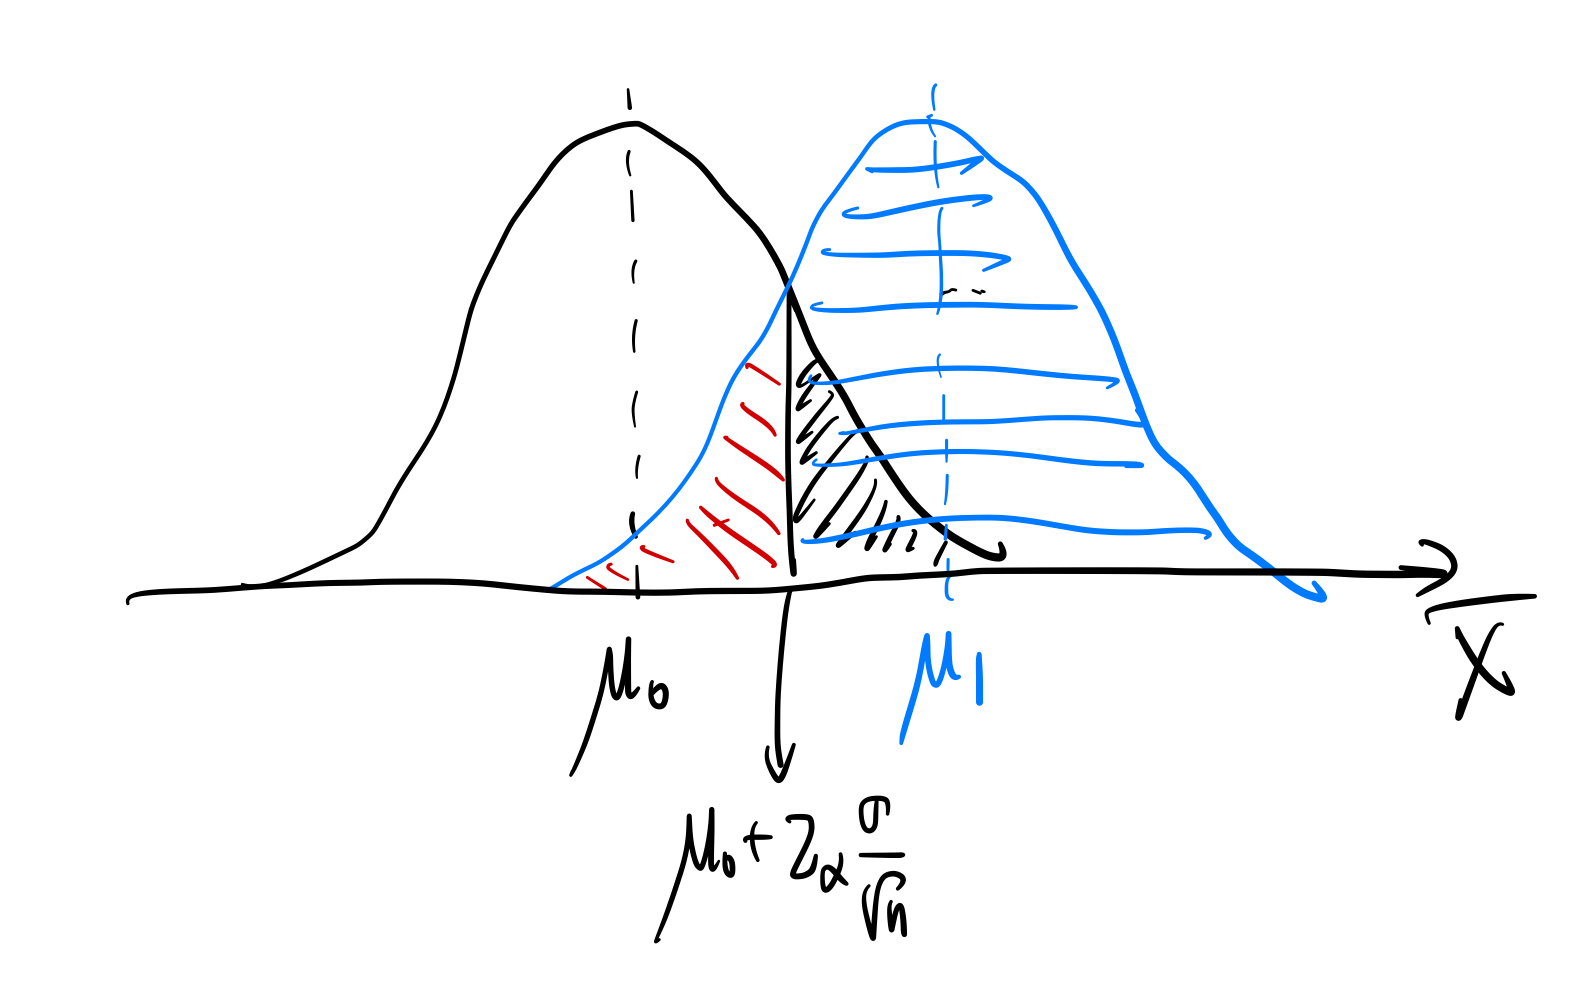
\includegraphics[width=0.8\textwidth]{figures/06-Hypothesis_testing/error_power.jpeg}
        \caption{檢定的型一錯誤率、型二錯誤率與檢定力}
        \label{fig:error_power}
    \end{figure}

    除了型一錯誤率外,我們的目的是要計算型二錯誤率(type II error rate, 常寫做 $\beta$),也就是對立假說成立下,無法拒絕虛無假說的機率。此時我們需要知道檢定統計量在對立假說成立下的抽樣分布,但我們的對立假說是 $\mu > 0$,並沒有一個明確的母體平均值。因此,我們要先設定一個對立假說下的母體平均值 $\mu_1$,以作為我們建立抽樣分布及後續計算型二錯誤率的參考。在這裡我們設定 $\mu_1 = 1$。若 $\mu = \mu_1 = 1$,$\bar{X}$ 的抽樣分布為 $\NN(\mu_1 = 1, \sigma^2/n = 1/9)$,我們將其描繪在圖 \ref{fig:error_power} 的藍色部分。型二錯誤率為對立假說成立下,無法拒絕虛無假說的機率,也就是 $\bar{X}$ 服從藍色的分布下,取值不足臨界值 0.55 的機率,即圖 \ref{fig:error_power} 中的紅色面積。這個面積的算法我們可以再次利用 z 轉換:
    \begin{align*}
        &\PP(\bar{X} < 0.55|H_1:\mu = 1) \\
        =& \PP(\bar{X} < 0.55|\bar{X} \sim \NN(1, 1/9))\\
        =& \PP\Big(\frac{\bar{X}-1}{1/3} < \frac{0.55 - 1}{1/3} \approx -1.35|\bar{X} \sim \NN(1, 1/9))\\
        =& \PP(\ZZ < -1.35) = \Phi(-1.35) \approx 0.089
    \end{align*}
    因此,我們知道當對立假說之參數取值為 $\mu = 1$ 時,檢定的型二錯誤率為 0.089。用白話來說,當母體平均實際上為 1 時,檢定「母體平均是否大於 0」卻無法拒絕虛無假說「母體平均等於 0」的機率為 0.089。這個機率越小,代表在無法拒絕虛無假說時,我們對於對立假說的信心越高。

    除了型二錯誤率以外,生醫統計上更常用的機率是它的反面:\textit{檢定力}(power)。檢定力是對立假說成立下,能夠成功拒絕虛無假說的機會。如圖\ref{tab:error_power}所示,檢定力即圖中藍色的面積(因為 $\bar{X}$ 在臨界值以上時,我們會拒絕虛無假說),因此檢定力恰等於一減去型二錯誤率。在上面的例子中,於對立假說成立且設定母體平均為 1 的情況下,該檢定的檢定力為 1-0.089 = 0.911。以白話來說,當母體平均實際上為 1 時,檢定「母體平均是否大於 0」並成功拒絕虛無假說「母體平均等於 0」的機率為 0.911。一般來說,我們希望檢定在控制型一錯誤率的前提下,檢定力能夠越大越好,我們才能有效率地判斷資料是否隱含著對立假設為真的訊息。
    
    為了瞭解什麼因素會影響檢定力,我們可以將符號重新帶回上述的所有計算,並得到單樣本母體平均值右尾檢定的檢定力公式:
    \[1-\beta = \Phi\Big(\frac{\mu_1-\mu_0}{\sigma/\sqrt{n}}-z_\alpha\Big) := \Phi\Big(\frac{\Delta}{\sigma/\sqrt{n}}-z_\alpha\Big)\]
    根據這個公式,我們可以分項探討各因素對於檢定力的導引方向:
    \begin{itemize}
        \item 效果量 $\Delta$:效果量定義為 $\mu_1-\mu_0$,即對立假說下母體平均取值與虛無假說的距離。效果量越大,檢定力也會越大。這個結果十分直覺:當對立假說下的母體平均遠大於虛無假說下的取值,那麼觀察到的樣本平均就會非常大,因此就有很大的機會拒絕虛無假說。
        \item 樣本數 $n$:當樣本數變大時,公式中的分母會變小,因此整體檢定力會變大。當樣本數變大時,資料中含有的資訊越多,我們就越有機會成功證偽虛無假說。
        \item 母體標準差 $\sigma$:當母體標準差變大時,公式中的分母會變大,因此整體檢定力會變小。母體標準差越大,代表每筆資料的資訊含量越低(可以想成測量誤差非常大,實際關於母題平均的資訊都被誤差稀釋掉了),因此成功證偽虛無假說的可能性就越低。
        \item 顯著水準(型一錯誤率) $\alpha$:通常我們不會任意調動顯著水準,但從公式可以看出,顯著水準調得越高,$z_\alpha$就會越小,因此整體檢定力就會越高。當我們把檢定的顯著水準調高,代表拒絕虛無假說的條件變得寬鬆,從而檢定力也會提高。如果用型一和型二錯誤率來看,可以知道型一錯誤率增高會讓型二錯誤率降低,反之亦然,兩者之間有一個權衡關係。
    \end{itemize}
    上述的討論中,我們雖然是用單樣本母體平均值右尾檢定作例子,但各因素對於檢定力的影響方向在各類檢定大致通用。

    檢定力公式除了可以用來計算檢定力外,另一個重要的用途是用來計算樣本數。我們一般都希望檢定的檢定力越大越好,但在檢定力公式中,母體標準差是資料的特性而無法更動,顯著水準有約定俗成的設定(通常是 0.05),而效果量則通常設定為臨床上有意義的效果差異(例如平均舒張壓下降 5 mmHg)。因此,研究者能夠隨意調動的通常只剩下樣本數,而做研究的第一步常需要了解樣本數應該要收到多少,才能夠讓檢定力達到一定水準,以求在做完研究後,如果檢定不顯著,我們還可以根據檢定力針對不顯著的結果作有信心的推論。樣本數的計算基本上就是將檢定力公式做反向推演。假設我們希望檢定力至少是 $1-\beta$(一般常設定為 0.8 或 0.9),那麼
    \[\Phi\Big(\frac{\Delta}{\sigma/\sqrt{n}}-z_\alpha\Big) \ge 1-\beta\]
    \[n \ge \Big[\frac{\sigma}{\Delta} (\Phi^{-1}(1-\beta) + z_\alpha)\Big]^2 = \Big(\frac{\sigma}{\Delta}\Big)^2(z_\alpha + z_\beta)^2\]
    一般而言實務上,考量到收進來的樣本可能會失去追蹤或是有測量失誤,因此會將樣本數設定為最低所需樣本數的倍數,例如 1.1 倍、1.25 倍等等。從這個公式可以看到,會使所需樣本數增加的因素為:母體標準差增加、所需偵測效果量降低、顯著水準上升、以及檢定力上升。這些影響方向的解釋原因和上述有關檢定力的討論類似,在這裡就不再贅述。
    
    \bigskip

    \begin{custom}{思考}
        在顯著水準維持不變的情況下,使用單尾檢定算出的樣本數應該比雙尾檢定算出的樣本數來得多還是來得少?
    \end{custom}

    \bigskip

    \begin{custom}{思考}
        若欲求比例單樣本檢定的樣本數,應該要提供那一些資訊以供計算?
    \end{custom}
    
    \begin{docexam}{(104-1醫學(一))}
        下面有關假說檢定之型一錯誤(type I error)與型二錯誤(type II error)的敘述何者正確?

        (A) 型一錯誤發生的機率加上型二錯誤發生的機率等於 1

        (B) 檢定力(power) = 1-型一錯誤的機率

        (C) 型一錯誤與型二錯誤有可能會同時發生

        (D) 固定型一錯誤的機率,增加樣本數可以降低型二錯誤發生的機率
    \end{docexam}
    
    \begin{docexam}{(107-1醫學(二))}
        進行統計檢定,當根據數據計算所得之 $p$ 值 > $\alpha$ (顯著水準)時,下列敘述何者正確?

        (A) 可以正確推翻虛無假設

        (B) 證據不足以推翻虛無假設

        (C) 可以正確接受虛無假設

        (D) 可能犯型 I 錯誤
    \end{docexam}

    % \bigskip
    
    % \begin{docexam}{(105-2醫學(一))}
    %     某麻醉科醫師想比較兩種麻醉藥物(舊藥與新藥)的效果,計畫收集採用舊藥50人及新藥50位病人在麻醉開始後至手術開始時的最小血壓值。麻醉科醫師希望可以偵測到兩組最小血壓值差距到 6 mmHg,下列何者做法可以提升統計假設檢定的檢定力 (power)?

    %     (A) 將檢定的顯著性水準由 0.05 增加至 0.1

    %     (B) 偵測到兩組最小血壓差距由 6 mmHg 降低到 3 mmHg

    %     (C) 樣本更改為收集舊藥 40 人及新藥 60 位病人

    %     (D) 樣本更改為收集舊藥 60 人及新藥 40 位病人
    % \end{docexam}
    
    \begin{docexam}{(105-1醫學(一))}
        兩種麻醉藥物死亡率差異的 $95\%$ 信賴區間為 (-0.142,0.102),若將檢定之顯著性水準由 0.05 更改為 0.01,其他條件不變下,檢定兩種麻醉藥物的死亡率是否有差異,下列敘述何者正確?

        (A) 兩種麻醉藥物的死亡率達統計顯著

        (B) 兩種麻醉藥物的死亡率未達統計顯著

        (C) 無法下結論

        (D) 此檢定的結果有可能犯下型一錯誤 (type I error)
    \end{docexam}
    
    \begin{docexam}{(104-2醫學(一))}
        下列哪一選項能夠增加統計檢定力(statistical power)?

        (A) 採用雙盲 (double-blind)

        (B) 隨機分派 (randomization)

        (C) 增加樣本數 (sample size)

        (D) 使用對照組 (control)
    \end{docexam}
    
    \begin{docexam}{(103-2醫學(一))}
        統計假說檢定(statistical hypothesis testing)時,何謂型二錯誤(type II error)?

        (A) 兩組實際上無差異,分析結果推翻虛無假說(null hypothesis)

        (B) 兩組實際上無差異,分析結果支持虛無假說

        (C) 兩組實際上有差異,分析結果推翻虛無假說

        (D) 兩組實際上有差異,分析結果支持虛無假說
    \end{docexam}
    
    \begin{docexam}{(103-2醫學(一))}
        一項研究探討中學生現在近視的比例 (m0) 是否高於 10 年前,如果 10 年前中學生的近視比例是 45\%,下列有關虛無假設 (null hypothesis, H0) 與對立假設 (alternative hypothesis, HA) 的敘述,何者正確?

        (A) H0: m0 = 0 vs HA: m0 $\ne$ 0

        (B) H0: m0 = 0.45 vs HA: m0 $\ne$ 0.45

        (C) H0: m0 $\ge$ 0.45 vs HA: m0 < 0.45

        (D) H0: m0 $\le$ 0.45 vs HA: m0 > 0.45
    \end{docexam}
    
    \begin{docexam}{(103-1醫學(一))}
        下列有關檢力(power)的敘述,何者正確?

        (A) 降低顯著水準,例如從 0.05 變成 0.01,檢力將變大

        (B) 如果對立假設的平均值,比預期更遠離虛無假設的平均值,則檢定的檢力將增加

        (C) 若觀測值的標準差增加,則檢力增加

        (D) 若樣本數減少,則檢力增加
    \end{docexam}
    
    \begin{docexam}{(101-2醫學(一))}
        在統計推論做雙尾檢定時,經計算得 $p$ 值為 0.04,若其他條件不變,改做單尾檢定,其 $p$ 值會有何種變化?

        (A) 變大

        (B) 變小

        (C) 如果變項是常態分布的情況下會變大,若不是則變小

        (D) 如果變項是常態分布的情況下會變小,若不是則變大
    \end{docexam}
    
    \begin{docexam}{(101-2醫學(一))}
        有關統計檢定,下列哪一項敘述錯誤?

        (A) 統計的 Power 係指可正確判斷新治療方式有效的機率

        (B) 統計的 Type I error 係指新治療方式無效,卻被判定為有效的機率

        (C) 統計的 Type I error 係指新治療方式無效,卻被判定為有效的機率

        (D) 統計的信賴水準 ($1-\alpha$) 係指新治療方式無效,可被正確判斷的機率
    \end{docexam}
    
    \begin{docexam}{(101-1醫學(一))}
        某小型臨床試驗評估一個新化療治療淋巴癌的療效,若事實上此新化療有比較好的療效,但本研究沒發現顯著的五年存活率差異,無法偵測此新治療效果的原因為何?

        (A) 檢力(power)太大

        (B) 抽樣誤差

        (C) 型一誤差(type I error)

        (D) 型二誤差(type II error)
    \end{docexam}
    
    \begin{docexam}{(101-1醫學(一))}
        甲醫院手術治療某種疾病,抽樣100個病人有80個治療成功,成功率的 95\% 信賴區間 (95\% confidence interval) 為 (0.72,0.88)。如果一般全國平均治療這種病人的成功率為 90\%,我們想以此資料來做假說檢定,檢定甲醫院治療此病成功率是否比 90\% 低,顯著水準設為 $\alpha$ = 0.05,下列何者正確?

        (A) 無法推翻虛無假說,結論是甲醫院的治療成功率與 95\% 一樣

        (B) 推翻虛無假說,結論是甲醫院的治療成功率比 90\% 低

        (C) 無法推翻虛無假說,結論是甲醫院的治療成功率比 90\% 低

        (D) 推翻虛無假說,結論是甲醫院的治療成功率與 90\% 一樣
    \end{docexam}
    
    \begin{docexam}{(100-1醫學(一))}
        當一個研究者結論未能偵測出顯著的效應,下列何者的誤差和研究者的結論有關聯?

        (A) 因為樣本數太小,此結論錯誤的可能性很低

        (B) 犯下第二誤差的可能性很小

        (C) 第一誤差的機率大於0.05

        (D) 犯下第二誤差的可能性很大
    \end{docexam}
    
    \begin{docexam}{(108-1醫學(二))}
        一研究想比較抽菸者與非抽菸者的血膽固醇濃度,下列敘述何者錯誤?

        (A) 檢定時犯下型一錯誤 (type I error) 的機率,即為研究者設定的顯著水準

        (B) 若顯著水準不變,欲增加統計檢定力,可以增加樣本數

        (C) 型一錯誤是抽菸者與非抽菸者的血膽固醇濃度沒差異,但檢定時卻誤判有差異的情形

        (D) 型一錯誤加型二錯誤的機率和為 $1$
    \end{docexam}
    
    \begin{docexam}{(108-2醫學(二))}
        統計假說檢定 (statistical hypothesis testing) 時,何謂型一錯誤 (type I error)?

        (A) 兩組實際上無差異,分析結果推翻虛無假說 (null hypothesis) 

        (B) 兩組實際上無差異,分析結果支持虛無假說 (null hypothesis) 

        (C) 兩組實際上有差異,分析結果推翻虛無假說 (null hypothesis) 

        (D) 兩組實際上有差異,分析結果支持虛無假說 (null hypothesis) 
    \end{docexam}
    
    \begin{docexam}{(108-2醫學(二))}
        有關單尾與雙尾假說檢定的敘述,下列何者正確?

        (A) 單尾與雙尾假說檢定的 $p$ 值算法相同

        (B) 相對於雙尾假說檢定,單尾假說檢定比較不易拒絕虛無假說

        (C) 單尾與雙尾假說檢定的顯著水準 ($\alpha$) 相同 

        (D) 相對於雙尾假說檢定,單尾假說檢定比較常被使用
    \end{docexam}

    \begin{docexam}{(112-1醫學(二))}
        醫療檢測數據呈現明顯右偏分布,下列何組指標最適合測量此群資料之集中與分散狀況?

        (A) 平均值,標準差

        (B) 平均值,標準誤

        (C) 中位數,四分位距

        (D) 中位數,全距
    \end{docexam}
    
\chapter{比較兩組樣本的假說檢定}

    前一章我們介紹了假說檢定的架構,以及如何檢定一組樣本背後的母體平均值(或母體比例)是否大於、等於、或小於我們預想的數值。然而,在生醫研究中,我們更常有興趣的是,從兩個母體各抽出一組樣本後,檢定背後兩個母體的平均值或是比例之間的關係。例如,在血壓藥物的隨機對照實驗中,我們將受試者隨機分為兩組並各給予不同的藥物治療。此時我們有興趣的是,接受兩種藥物治療後的平均血壓是否有差別,進而推論兩種藥物的效果優劣。因此,本章我們將著重探討如何針對兩組樣本的母體平均值(或母體比例)差異作檢定,以及如何為這個差異建構信賴區間。
    
    \begin{introduction}[第 \thechapter 章學習目標]
        \item 在各種母體假設下,利用 $Z$ 及 $t$ 檢定比較兩組樣本的母體平均
        \item 檢定比較兩組樣本的母體比例
        \item 母體平均差值及母體比例差值的信賴區間建構
    \end{introduction}

\section{母體平均的獨立雙樣本檢定:兩個母體均為常態分布且變異數已知}

    我們首先討論如何比較兩組常態樣本背後之母體平均。假設已知兩個母體均服從常態分布且互相獨立。兩者母體平均未知,分別記為 $\mu_1$ 和 $\mu_2$,但變異數均已知,分別為 $\sigma_1^2$ 和 $\sigma_2^2$。若將兩組樣本的樣本平均記為 $\bar{X}_1, \bar{X}_2$,則其抽樣分布應分別為
    \[\bar{X}_1 \sim \NN\Big(\mu_1, \frac{\sigma_1^2}{n_1}\Big) \qquad ; \qquad \bar{X}_2 \sim \NN\Big(\mu_2, \frac{\sigma_2^2}{n_2}\Big)\]
    由於兩組樣本互相獨立,因此兩個樣本平均也互相獨立。將兩個樣本平均相減後,期望值亦為相減,變異數則因獨立而為相加:
    \[\bar{X}_2-\bar{X}_1 \sim \NN \Big(\mu_2 - \mu_1, \frac{\sigma_1^2}{n_1} + \frac{\sigma_2^2}{n_2}\Big)\]
    由於 $\bar{X}_2-\bar{X}_1$ 服從常態分布,我們可以將其做 $z$ 轉換,轉換後即服從標準常態分布
    \[\frac{(\bar{X}_2-\bar{X}_1)-(\mu_2-\mu_1)}{\sqrt{\frac{\sigma_1^2}{n_1} + \frac{\sigma_2^2}{n_2}}} \sim \ZZ\]
    此時根據虛無假說和對立假說的形式,我們可以對 $\mu_2-\mu_1$ 的數值建構檢定。為了簡單起見,我們假定虛無假說都是 $H_0: \mu_2 = \mu_1$ 的形式,也就是在虛無假說下兩個母體的平均相等。如此一來,在虛無假說下,以下 $Z$ 檢定量的虛無分布為標準常態分布:
    \[Z := \frac{\bar{X}_2-\bar{X}_1}{\sqrt{\frac{\sigma_1^2}{n_1} + \frac{\sigma_2^2}{n_2}}} \sim \ZZ\]
    對立假說隨著 $\mu_2-\mu_1$ 的方向不同而決定其為右尾、左尾或雙尾檢定。若設定為 $H_1: \mu_2 > \mu_1$ 則為右尾檢定;若設定為 $H_1: \mu_2 < \mu_1$ 則為左尾檢定;若設定為 $H_1: \mu_2 \ne \mu_1$ 則為雙尾檢定。

    \noindent\underline{\textbf{右尾檢定}}

    右尾檢定的假說形如 $H_0: \; \mu_2 = \mu_1 \; ; \; H_1: \; \mu_2 > \mu_1$。我們可以用 $p$ 值法來建構檢定:當對立假說為真時,$\bar{X}_2 - \bar{X}_1$ 的期望值 $\mu_2 - \mu_1$ 會大於 0,因此 $Z$ 偏大的方向是比較「極端」的方向。根據 $p$ 值的定義可以寫出
    \[p = \PP(\ZZ \ge Z)\]
    此時若 $p \le \alpha$ 則拒絕虛無假說、接受對立假說;反之則無法拒絕虛無假說。同樣地,我們也可以用拒絕域法建構檢定而得到拒絕區為 $Z \ge z_\alpha$,統計量臨界值為 $z_\alpha$。

    \noindent\underline{\textbf{左尾檢定}}

    若假說形如 $H_0: \; \mu_2 = \mu_1 \; ; \; H_1: \; \mu_2 < \mu_1$,我們可以用 $p$ 值法來建構檢定:當對立假說為真時,$\bar{X}_2 - \bar{X}_1$ 的期望值 $\mu_2 - \mu_1$ 會小於 0,因此 $Z$ 偏小的方向是比較「極端」的方向。根據 $p$ 值的定義可以寫出
    \[p = \PP(\ZZ \le Z)\]
    此時若 $p \le \alpha$ 則拒絕虛無假說、接受對立假說;反之則無法拒絕虛無假說。同樣地,我們也可以用拒絕域法建構檢定而得到拒絕區為 $Z \le z_\alpha$,統計量臨界值為 $z_\alpha$。

    \noindent\underline{\textbf{雙尾檢定}}

    若假說形如 $H_0: \; \mu_2 = \mu_1 \; ; \; H_1: \; \mu_2 \ne \mu_1$,我們可以用 $p$ 值法來建構檢定:當對立假說為真時,$\bar{X}_2 - \bar{X}_1$ 的期望值 $\mu_2 - \mu_1$ 會往兩側遠離 0,因此 $Z$ 不論偏大或偏小都是「極端」的方向。且因為 $Z$ 的虛無分布期望值為零,$Z$ 和 $-Z$ 的極端程度是一樣的。因此,根據 $p$ 值的定義可以寫出
    \[p = \PP((\ZZ \ge |Z|)\cup(\ZZ \le -|Z|)) = 2\PP(\ZZ \ge |Z|)\]
    此時若 $p \le \alpha$ 則拒絕虛無假說、接受對立假說;反之則無法拒絕虛無假說。同樣地,我們也可以用拒絕域法建構檢定而得到拒絕區為 $|Z| \ge z_{\alpha/2}$,統計量臨界值為 $\pm z_{\alpha}$ 。

    以下我們用表 \ref{tab:two_sample_z} 來整理母體服從常態分布且變異數已知的母體平均雙樣本檢定。由於此檢定比較了兩組獨立樣本,且是用 $Z$ 檢定統計量來建構,統計量的虛無分布為標準常態分布($\ZZ$),因此此檢定亦稱為\textit{獨立樣本 Z 檢定} (Independent sample Z test) 或\textit{雙樣本 Z 檢定} (Two-sample Z test)。

    \begin{table}[htbp]
        \begin{center}
            \begin{tabular}{ccccc}
                \toprule
                虛無假說($H_0$) & 對立假說($H_1$) & 檢定統計量 & $p$ 值 & 拒絕區\\
                \hline
                \multirow{3}{*}{$\mu_2 = \mu_1$} & $\mu_2 > \mu_1$ & \multirow{3}{*}{$Z = \frac{\bar{X}_2-\bar{X}_1}{\sqrt{\frac{\sigma_1^2}{n_1}+\frac{\sigma_2^2}{n_2}}}$} & $\PP(\ZZ \ge Z)$ & $Z \ge z_{\alpha}$\\
                & $\mu_2 < \mu_1$ & &$\PP(\ZZ \le Z)$&$Z \le -z_{\alpha}$\\
                & $\mu_2 \ne \mu_1$ & &$2\times\PP(\ZZ \ge |Z|)$&$|Z| \ge z_{\alpha/2}$\\
                \bottomrule
            \end{tabular}
            \caption{母體為常態分布且變異數已知的母體平均雙樣本檢定(雙樣本 Z 檢定)\label{tab:two_sample_z}}
        \end{center}
    \end{table}

    除了進行檢定外,我們也可以根據 $\bar{X}_2 - \bar{X}_1$ 作 $z$ 轉換後的抽樣分布,建構母體平均差 $\mu_2 - \mu_1$ 的信賴區間。以 $(1-\alpha) \times 100\%$ 雙尾信賴區間為例,因為 $\frac{(\bar{X}_2-\bar{X}_1)-(\mu_2-\mu_1)}{\sqrt{\frac{\sigma_1^2}{n_1} + \frac{\sigma_2^2}{n_2}}} \sim \ZZ$,
    \[\PP\Bigg(-z_{\alpha/2} < \frac{(\bar{X}_2-\bar{X}_1)-(\mu_2-\mu_1)}{\sqrt{\frac{\sigma_1^2}{n_1} + \frac{\sigma_2^2}{n_2}}} < z_{\alpha/2}\Bigg) = 1-\alpha\]
    \[\PP\Bigg[(\bar{X}_2-\bar{X}_1) - z_{\alpha/2} \sqrt{\frac{\sigma_1^2}{n_1} + \frac{\sigma_2^2}{n_2}} < \mu_2-\mu_1  < (\bar{X}_2-\bar{X}_1) + z_{\alpha/2} \sqrt{\frac{\sigma_1^2}{n_1} + \frac{\sigma_2^2}{n_2}}\Bigg] = 1-\alpha\]
    因此,$\mu_2-\mu_1$ 的 $(1-\alpha) \times 100\%$ \textbf{雙尾}信賴區間即為
    \[\Bigg((\bar{X}_2-\bar{X}_1) - z_{\alpha/2} \sqrt{\frac{\sigma_1^2}{n_1} + \frac{\sigma_2^2}{n_2}},  (\bar{X}_2-\bar{X}_1) + z_{\alpha/2} \sqrt{\frac{\sigma_1^2}{n_1} + \frac{\sigma_2^2}{n_2}}\Bigg)\]
    根據我們上一章有關檢定與信賴區間之間關係的探討,當這個雙尾信賴區間未覆蓋到 $0$ 時,等同於在顯著水準 $\alpha$ 下拒絕 $\mu_2 - \mu_1 = 0$ 的虛無假說,並接受 $\mu_2 \ne \mu_1$ 的\textbf{雙尾}對立假說。同理,$\mu_2-\mu_1$ 的 $(1-\alpha) \times 100\%$ 右尾及左尾信賴區間分別為
    \[\Bigg((\bar{X}_2-\bar{X}_1) - z_{\alpha} \sqrt{\frac{\sigma_1^2}{n_1} + \frac{\sigma_2^2}{n_2}}, \infty \Bigg) \quad ; \quad \Bigg(-\infty, (\bar{X}_2-\bar{X}_1) + z_{\alpha} \sqrt{\frac{\sigma_1^2}{n_1} + \frac{\sigma_2^2}{n_2}} \Bigg)\]
    前者未覆蓋到 $0$ 則可接受 $\mu_2 > \mu_1$ 的對立假說,後者未覆蓋到 $0$ 則可接受 $\mu_2 < \mu_1$ 的對立假說。
    
\section{母體平均的獨立雙樣本檢定:兩個母體均為常態分布但變異數未知}

    上一節我們假設了兩個母體均為常態分布且變異數均已知,因此可以將樣本平均的差 $\bar{X}_2-\bar{X}_1$ 進行 $z$ 轉換,且得到在兩母體平均相等($H_0: \mu_1 = \mu_0$)的虛無假說下
    \[Z := \frac{\bar{X}_2-\bar{X}_1}{\sqrt{\frac{\sigma_1^2}{n_1} + \frac{\sigma_2^2}{n_2}}} \sim \ZZ\]
    當變異數未知時,$\sigma_1^2$ 和 $\sigma_2^2$ 均為未知數,因此無法計算 $Z$ 統計量。此時,按照我們之前在單樣本檢定的經驗,我們會希望能以兩組的樣本變異數 $s_1^2$ 和 $s_2^2$ 帶入 $\sigma_1^2$ 和 $\sigma_2^2$,並希望帶入後的統計量能夠是我們熟知的分布(在單樣本的例子是自由度為樣本數減一的 $t$ 分布)。然而事與願違,如此帶入後得到的檢定量並不完全服從 $t$ 分布,僅能根據統計學家 Bernard Lewis Welch (1911–29) 提出的方法,用一個自由度十分複雜的 $t$ 分布來近似該統計量的虛無分布,此檢定也被稱為 \textit{Welch $t$ 檢定} (Welch $t$ test),在大多數統計軟體套件均有提供:
    \[t^* := \frac{\bar{X}_2-\bar{X}_1}{\sqrt{\frac{s_1^2}{n_1} + \frac{s_2^2}{n_2}}} \sim t_\nu \quad; \quad \nu \approx \frac{(s_1^2/n_1+s_2^2/n_2)^2}{s_1^4/n_1^2(n_1-1) +s_2^4/n_2^2(n_2-1)}\]
    除了使用含有近似成分的 Welch $t$ 檢定外,如果我們願意新增一個「\textbf{兩個母體變異數相等}」假設,那麼就可以建構一個精確的 $t$ 檢定。當兩組的母體變異數均為 $\sigma^2$,原本的 $Z$ 統計量就可寫為
    \[Z := \frac{\bar{X}_2-\bar{X}_1}{\sqrt{\sigma^2\big(\frac{1}{n_1} + \frac{1}{n_2}\big)}}\]
    此時因為兩個母體變異數相等,兩組的樣本變異數 $s_1^2$ 和 $s_2^2$ 都是母體變異數 $\sigma^2$ 的不偏估計量,但其準確度則取決於兩者的自由度 $n_1-1$ 和 $n_2-1$:自由度越大,準確度越大。因此,我們可以將 $s_1^2$ 和 $s_2^2$ 取加權平均,權重和兩者的自由度成正比而得到\textit{合併變異數估計值} (pooled variance estimate):
    \[s_{\text{pooled}}^2 = \frac{(n_1-1)s_1^2 + (n_2-1)s_2^2}{n_1+n_2-2}\]
    而後我們可以將合併變異數估計值帶入 $Z$ 檢定量中未知的 $\sigma^2$ 而得到 $t$ 檢定統計量:
    \[ t := \frac{\bar{X}_2-\bar{X}_1}{\sqrt{s_{\text{pooled}}^2\big(\frac{1}{n_1} + \frac{1}{n_2}\big)}} \sim t_{n_1+n_2-2}\]    
    此統計量在 $H_0: \mu_2 = \mu_1$ 下的虛無分布為自由度等於 $n_1 + n_2 - 2$ 的 $t$ 分布。這裡 $t$ 分布的自由度和先前單樣本的想法相同,取決於分母計算變異數時,使用的樣本數減去估計的參數個數。此處總樣本數為 $n_1+n_2$,但在計算 $s_1^2$ 和 $s_2^2$ 時各估計了一個組內的平均值,所以需要減去 $2$,從而得到 $n_1 + n_2 - 2$ 的自由度。
    
    根據上述的 $t$ 統計量,我們可以根據對立假設的方向建構右尾、左尾與雙尾檢定:
    
    \noindent\underline{\textbf{右尾檢定}}

    右尾檢定的假說形如 $H_0: \; \mu_2 = \mu_1 \; ; \; H_1: \; \mu_2 > \mu_1$。我們先用 $p$ 值法來建構檢定:當對立假說為真時,$\bar{X}_2 - \bar{X}_1$ 的期望值 $\mu_2 - \mu_1$ 會大於 0,因此 $t$ 偏大的方向是比較「極端」的方向。根據 $p$ 值的定義可以寫出
    \[p = \PP(t_{n_1+n_2-2} \ge t)\]
    此時若 $p \le \alpha$ 則拒絕虛無假說、接受對立假說;反之則無法拒絕虛無假說。同樣地,我們也可以用拒絕域法建構檢定而得到拒絕區為 $t \ge t_{n_1+n_2-2,\alpha}$,統計量臨界值為 $t_{n_1+n_2-2,\alpha}$。

    \noindent\underline{\textbf{左尾檢定}}

    若假說形如 $H_0: \; \mu_2 = \mu_1 \; ; \; H_1: \; \mu_2 < \mu_1$,我們仍先用 $p$ 值法來建構檢定:當對立假說為真時,$\bar{X}_2 - \bar{X}_1$ 的期望值 $\mu_2 - \mu_1$ 會小於 0,因此 $t$ 偏小的方向是比較「極端」的方向。根據 $p$ 值的定義可以寫出
    \[p = \PP(t_{n_1+n_2-2} \le t)\]
    此時若 $p \le \alpha$ 則拒絕虛無假說、接受對立假說;反之則無法拒絕虛無假說。同樣地,我們也可以用拒絕域法建構檢定而得到拒絕區為$t \le -t_{n_1+n_2-2,\alpha}$,統計量臨界值為 $-t_{n_1+n_2-2,\alpha}$。

    \noindent\underline{\textbf{雙尾檢定}}

    若假說形如 $H_0: \; \mu_2 = \mu_1 \; ; \; H_1: \; \mu_2 \ne \mu_1$,我們用 $p$ 值法來建構檢定:當對立假說為真時,$\bar{X}_2 - \bar{X}_1$ 的期望值 $\mu_2 - \mu_1$ 會往兩側遠離 0,因此 $t$ 不論偏大或偏小都是「極端」的方向。且因為 $t$ 的虛無分布期望值為零,$t$ 和 $-t$ 的極端程度是一樣的。因此,根據 $p$ 值的定義可以寫出
    \[p = \PP((t_{n_1+n_2-2} \ge |t|)\cup(t_{n_1+n_2-2} \le -|t|)) = 2\PP(t_{n_1+n_2-2} \ge |t|)\]
    此時若 $p \le \alpha$ 則拒絕虛無假說、接受對立假說;反之則無法拒絕虛無假說。我們也可以用拒絕域法建構檢定而得到拒絕區 $|t| \ge t_{n_1+n_2-2,\alpha/2}$,統計量臨界值為 $\pm t_{n_1+n_2-2,\alpha/2}$ 。
    
    以下我們用表 \ref{tab:two_sample_t} 來整理母體服從常態分布且變異數未知的母體平均雙樣本檢定。因為這個檢定是利用 $t$ 分布和兩組獨立樣本做的檢定,因此常被稱為\textit{獨立樣本 $t$ 檢定} (independent $t$-test)或\textit{雙樣本 $t$ 檢定} (two-sample $t$-test):

    \begin{table}[htbp]
        \begin{center}
            \begin{tabular}{ccccc}
                \toprule
                虛無假說($H_0$) & 對立假說($H_1$) & 檢定統計量 & $p$ 值 & 拒絕區\\
                \hline
                \multirow{3}{*}{$\mu_2 = \mu_1$} & $\mu_2 > \mu_1$ & \multirow{3}{*}{$t = \frac{\bar{X}_2-\bar{X}_1}{\sqrt{s_{\text{pooled}}^2\big(\frac{1}{n_1} + \frac{1}{n_2}\big)}}$} & $\PP(t_{n_1+n_2-2} \ge t)$ & $t \ge t_{n_1+n_2-2,\alpha}$\\
                & $\mu_2 < \mu_1$ & &$\PP(t_{n_1+n_2-2} \le t)$&$t \le -t_{n_1+n_2-2,\alpha}$\\
                & $\mu_2 \ne \mu_1$ & &$2\times\PP(t_{n_1+n_2-2} \ge |t|)$&$|t| \ge t_{n_1+n_2-2,\alpha/2}$\\
                \bottomrule
            \end{tabular}
            \caption{母體為常態分布且變異數未知的母體平均雙樣本檢定(雙樣本 $t$ 檢定)\label{tab:two_sample_t}}
        \end{center}
    \end{table}

    如同前一節所述,我們也可以用 $t$ 分布建構母體平均差 $\mu_2 - \mu_1$ 的信賴區間。以 $(1-\alpha) \times 100\%$ 雙尾信賴區間為例,因為 $\frac{(\bar{X}_2-\bar{X}_1)-(\mu_2-\mu_1)}{\sqrt{s_{\text{pooled}}^2\big(\frac{1}{n_1} + \frac{1}{n_2}\big)}} \sim t_{n_1+n_2-2}$,
    \[\PP\Bigg(-t_{n_1+n_2-2,\alpha/2} < \frac{(\bar{X}_2-\bar{X}_1)-(\mu_2-\mu_1)}{\sqrt{s_{\text{pooled}}^2\big(\frac{1}{n_1} + \frac{1}{n_2}\big)}} < t_{n_1+n_2-2,\alpha/2}\Bigg) = 1-\alpha\]
    \[\PP\Bigg[(\bar{X}_2-\bar{X}_1) - t_{n_1+n_2-2,\alpha/2} \sqrt{s_{\text{pooled}}^2\Big(\frac{1}{n_1} + \frac{1}{n_2}\Big)} < \mu_2-\mu_1  < (\bar{X}_2-\bar{X}_1) + t_{n_1+n_2-2,\alpha/2} \sqrt{s_{\text{pooled}}^2\Big(\frac{1}{n_1} + \frac{1}{n_2}\Big)}\Bigg] = 1-\alpha\]
    因此,$\mu_2-\mu_1$ 的 $(1-\alpha) \times 100\%$ \textbf{雙尾}信賴區間即為
    \[\Bigg((\bar{X}_2-\bar{X}_1) - t_{n_1+n_2-2,\alpha/2} \sqrt{s_{\text{pooled}}^2\Big(\frac{1}{n_1} + \frac{1}{n_2}\Big)}, (\bar{X}_2-\bar{X}_1) + t_{n_1+n_2-2,\alpha/2} \sqrt{s_{\text{pooled}}^2\Big(\frac{1}{n_1} + \frac{1}{n_2}\Big)}\Bigg)\]
    當這個雙尾信賴區間未覆蓋到 $0$ 時,等同於在顯著水準 $\alpha$ 下拒絕 $\mu_2 - \mu_1 = 0$ 的虛無假說,並接受 $\mu_2 \ne \mu_1$ 的\textbf{雙尾}對立假說。同理,$\mu_2-\mu_1$ 的 $(1-\alpha) \times 100\%$ 右尾及左尾信賴區間分別為:
    \[\Bigg((\bar{X}_2-\bar{X}_1) - t_{n_1+n_2-2,\alpha} \sqrt{s_{\text{pooled}}^2\Big(\frac{1}{n_1} + \frac{1}{n_2}\Big)}, \infty \Bigg)\quad ; \quad\Bigg(-\infty, (\bar{X}_2-\bar{X}_1) + t_{n_1+n_2-2,\alpha} \sqrt{s_{\text{pooled}}^2\Big(\frac{1}{n_1} + \frac{1}{n_2}\Big)} \Bigg)\]
    前者未覆蓋到 $0$ 則可接受 $\mu_2 > \mu_1$ 的對立假說,後者未覆蓋到 $0$ 則可接受 $\mu_2 < \mu_1$ 的對立假說。
    
    理論上,使用 Welch $t$ 檢定不論在兩組母體變異數相等或不相等時都能得到(近似)正確的檢定結論,因此兩個獨立樣本的母體平均值檢定應可直接使用 Welch $t$ 檢定。但實務上,只要母體變異數不要相差太大,Welch $t$ 檢定和雙樣本 $t$ 檢定的結論會相似,因此兩者之間的選擇影響不大。

    \bigskip

    \begin{custom}{練習}
       某藥廠為比較其開發之新血壓藥 A 與鈣離子通道阻斷劑降低舒張壓之能力,將 36 名高血壓病患隨機分派至新血壓藥組與鈣離子通道阻斷劑組,各為 18 位。一個月後,新血壓藥 A 之病患平均舒張壓與標準差為 85 mmHg (5.1 mmHg),鈣離子通道阻斷劑之病患平均舒張壓與標準差為 82 mmHg (4.9 mmHg)。假設各組治療後糖化血色素之分布均為常態分布且母體變異相同,在顯著水準設定為 0.05 下,新血壓藥 A 之舒張壓下降效果是否鈣離子通道阻斷劑來得好?
    \end{custom}
    
    \bigskip

    \begin{custom}{練習}
       GLP-1 agonist 與 SGLT2 inhibitor 為控制糖尿病的兩大類藥物。Frías 等人為了解比較同時使用兩種藥物與單用一種藥物的血糖降低效果,將 695 位使用 Metformin 治療但血糖控制不佳的第二型糖尿病病患隨機分派至三種治療(括號內為實際完成並納入分析之病患人數):Exenatide 合併 Dapagliflozin (n=193)、單用Exenatide (n=184)、以及單用 dapagliflozin (n=196) (Frías et al. (2016). Exenatide once weekly plus dapagliflozin once daily versus exenatide or dapagliflozin alone in patients with type 2 diabetes inadequately controlled with metformin monotherapy (DURATION-8): a 28 week, multicentre, double-blind, phase 3, randomised controlled trial. The lancet Diabetes \& endocrinology, 4(12), 1004-1016.)。其中 Exenatide 為 GLP-1 agonist、Dapagliflozin 為 SGLT2 inhibitor。治療前三組之平均糖化血色素均為 9.3\%,治療後三組各別之平均糖化血色素與標準差分別為 7.2\% (1.3\%)、7.6\% (1.3\%) 與 7.7\% (1.1\%)。假設各組治療後糖化血色素之分布均為常態分布且母體變異相同,在顯著水準設定為 0.05 下,合併使用藥物之血糖下降效果是否與單用 GLP-1 agonist 有差異,差異之信賴區間為何?合併使用藥物之血糖下降效果是否與單用 SGLT2 inhibitor 有差異,差異之信賴區間為何?
    \end{custom}

\section{母體平均的配對雙樣本檢定}
    前面針對兩組樣本的母體平均進行比較時,均假設兩個樣本之間是獨立的。例如在比較 A 和 B 兩種藥物的隨機對照實驗中,接受 A 藥的病患和接受 B 藥的病患是相異的兩群人,所以資料中服用 A 藥後的平均結果和服用 B 藥後的平均結果是來自不同的病患,因而互相獨立。然而實際資料中,有可能兩組樣本均來自相同的受試者。例如,假定我們想知道服用 C 藥一個月平均而言是否會讓舒張壓下降,因此募集了一群高血壓病患先行測量服藥前的舒張壓,並在服用 C 藥一個月後再次測量舒張壓,資料舉例如表 \ref{tab:paired_data}。此時我們有兩組樣本,一組是服藥前的舒張壓、一組是服藥後的舒張壓,但這兩組樣本並不獨立,因為它們都來自同樣一群高血壓病患。更精確地來說,這兩組樣本其實有個 \textbf{一一對應} 的關係,每位病患都會貢獻一筆服藥前的血壓、以及一筆服藥後的血壓,而這兩個血壓值並不是獨立的(服藥前的血壓會影響到服藥後的血壓)。因此,此處我們不能使用雙樣本 $t$ 檢定來決定服藥前後的平均血壓是否相等。

    解決上述配對樣本資料相依的方法十分簡單:我們的目的是想對服藥前後的平均血壓差異做推論,因此只要先行算出每位病患的服藥前後血壓差,再對算出來的血壓差作單樣本的母體平均檢定即可。換言之,表\ref{tab:paired_data}中,治療前和治療後兩個 column 的樣本平均因為來自於配對資料而不獨立,但我們可以將兩者的差值先行算出來,則該差值的母體平均大於、等於或小於 $0$ 就代表代表治療前的舒張壓大於、等於或小於治療後的舒張壓。而檢定該差值母體平均的方法,即可運用上一章所提到單樣本 $t$ 檢定。這個方法因為是用來處理配對資料,所以也被稱為\textit{配對 $t$ 檢定} (paired $t$-test),它本質上其實就是一個單樣本的 $t$ 檢定,只是處理的樣本來自配對資料中每個個體的前後差異。

    \begin{table}[htbp]
        \begin{center}
            \begin{tabular}{ccccc}
                \toprule
                病患編號 & 治療前 & 治療後 & 差值 \\
                \hline
                1 & 93 & 87 & 6 \\
                2 & 95 & 90 & 5 \\
                3 & 92 & 89 & 3 \\
                $\vdots$ & $\vdots$ & $\vdots$ & $\vdots$ \\
                \bottomrule
            \end{tabular}
            \caption{配對資料的例子演示\label{tab:paired_data}}
        \end{center}
    \end{table}

\section{母體比例的獨立雙樣本檢定}
    我們前面提到的雙樣本檢定都僅限於有興趣的變項服從常態分布時才適用。然而,當我們有興趣的變項是二元變項,例如疾病發病與否,並且想比較兩個獨立樣本間發病機率的差異時,仍然可以運用中央極限定理以及前述的獨立樣本雙樣本檢定來進行推論。如同上一章所說明,在樣本數夠大的情況下,兩組樣本的樣本發病機率 $\hat{p}_1$ 和 $\hat{p}_2$ 之抽樣分布可寫為
    \[\hat{p}_1 \xrightarrow[]{d} \NN\Big(p_1, \frac{p_1(1-p_1)}{n_1}\Big) \quad ; \quad \hat{p}_2 \xrightarrow[]{d} \NN\Big(p_2, \frac{p_2(1-p_2)}{n_2}\Big)\]
    由於兩組樣本互相獨立,因此樣本發病機率之差的抽樣分布可寫為
    \[\hat{p}_2 - \hat{p}_1 \xrightarrow[]{d} \NN\Big(p_2 - p_1, \frac{p_1(1-p_1)}{n_1} + \frac{p_2(1-p_2)}{n_2}\Big)\]
    在虛無假說為 $H_0 : p_2 = p_1 = \bar{p}$,也就是兩組樣本之母體比例相等的情況下,我們可以對 $\hat{p}_2 - \hat{p}_1$ 作 $z$ 轉換並得到
    \[Z:=\frac{\hat{p}_2 - \hat{p}_1}{\sqrt{\bar{p}(1-\bar{p})\big(\frac{1}{n_1} + \frac{1}{n_2}\big)}} \xrightarrow[]{d} \ZZ\]
    其中左側的統計量中,我們不知道共通母體比例 $\bar{p}$ 的數值,但我們知道在虛無假說下它同時是兩組的母體比例,因此可以將兩組資料合併後計算一個統整的樣本發病機率並帶入之,也就是
    \[\bar{p} = \frac{n_1\hat{p}_1 + n_2\hat{p}_2}{n_1+n_2}\]
    
    根據上面的 $Z$ 統計量,我們可以根據對立假說的方向建立假說檢定:

    \noindent\underline{\textbf{右尾檢定}}

    右尾檢定的假說形如 $H_0: \; p_2 = p_1 \; ; \; H_1: \; p_2 > p_1$。我們可以用 $p$ 值法來建構檢定:當對立假說為真時,$\hat{p}_2 - \hat{p}_1$ 的期望值 $p_2 - p_1$ 會大於 0,因此 $Z$ 偏大的方向是比較「極端」的方向。根據 $p$ 值的定義可以寫出
    \[p = \PP(\ZZ \ge Z)\]
    此時若 $p \le \alpha$ 則拒絕虛無假說、接受對立假說;反之則無法拒絕虛無假說。同樣地,我們也可以用拒絕域法建構檢定而得到拒絕區為 $Z \ge z_\alpha$,統計量臨界值為 $z_\alpha$。

    \noindent\underline{\textbf{左尾檢定}}

    若假說形如 $H_0: \; p_2 = p_1 \; ; \; H_1: \; p_2 < p_1$,我們可以用 $p$ 值法來建構檢定:當對立假說為真時,$\hat{p}_2 - \hat{p}_1$ 的期望值 $p_2 - p_1$ 會小於 0,因此 $Z$ 偏小的方向是比較「極端」的方向。根據 $p$ 值的定義可以寫出
    \[p = \PP(\ZZ \le Z)\]
    此時若 $p \le \alpha$ 則拒絕虛無假說、接受對立假說;反之則無法拒絕虛無假說。同樣地,我們也可以用拒絕域法建構檢定而得到拒絕區為 $Z \le z_\alpha$,統計量臨界值為 $z_\alpha$。

    \noindent\underline{\textbf{雙尾檢定}}

    若假說形如 $H_0: \; p_2 = p_1 \; ; \; H_1: \; p_2 \ne p_1$,我們可以用 $p$ 值法來建構檢定:當對立假說為真時,$\hat{p}_2 - \hat{p}_1$ 的期望值 $p_2 - p_1$ 會往兩側遠離 0,因此 $Z$ 不論偏大或偏小都是「極端」的方向。且因為 $Z$ 的虛無分布期望值為零,$Z$ 和 $-Z$ 的極端程度是一樣的。因此,根據 $p$ 值的定義可以寫出
    \[p = \PP((\ZZ \ge |Z|)\cup(\ZZ \le -|Z|)) = 2\PP(\ZZ \ge |Z|)\]
    此時若 $p \le \alpha$ 則拒絕虛無假說、接受對立假說;反之則無法拒絕虛無假說。同樣地,我們也可以用拒絕域法建構檢定而得到拒絕區為 $|Z| \ge z_{\alpha/2}$,統計量臨界值為 $\pm z_{\alpha}$ 。

    以下我們用表 \ref{tab:two_sample_proportion} 來整理母體比例的獨立雙樣本檢定。

    \begin{table}[htbp]
        \begin{center}
            \begin{tabular}{ccccc}
                \toprule
                虛無假說($H_0$) & 對立假說($H_1$) & 檢定統計量 & $p$ 值 & 拒絕區\\
                \hline
                \multirow{3}{*}{$p_2 = p_1$} & $p_2 > p_1$ & \multirow{3}{*}{$Z = \frac{\hat{p}_2-\hat{p}_1}{\sqrt{\bar{p}(1-\bar{p})\big(\frac{1}{n_1} + \frac{1}{n_2}\big)}}$} & $\PP(\ZZ \ge Z)$ & $Z \ge z_{\alpha}$\\
                & $p_2 < p_1$ & &$\PP(\ZZ \le Z)$&$Z \le -z_{\alpha}$\\
                & $p_2 \ne p_1$ & &$2\times\PP(\ZZ \ge |Z|)$&$|Z| \ge z_{\alpha/2}$\\
                \bottomrule
            \end{tabular}
            \caption{母體比例的獨立雙樣本檢定\label{tab:two_sample_proportion}}
        \end{center}
    \end{table}

    除了進行檢定外,我們也可以根據 $\hat{p}_2 - \hat{p}_1$ 作 $z$ 轉換後的抽樣分布,建構母體比例差值 $p_2 - p_1$ 的信賴區間。以 $(1-\alpha) \times 100\%$ 雙尾信賴區間為例,因為 $\frac{(\hat{p}_2-\hat{p}_1)-(p_2-p_1)}{\sqrt{\frac{p_1(1-p_1)}{n_1} + \frac{p_2(1-p_2)}{n_2}}} \sim \ZZ$,
    \[\PP\Bigg(-z_{\alpha/2} < \frac{(\hat{p}_2-\hat{p}_1)-(p_2-p_1)}{\sqrt{\frac{p_1(1-p_1)}{n_1} + \frac{p_2(1-p_2)}{n_2}}} < z_{\alpha/2}\Bigg) = 1-\alpha\]
    \[\PP\Bigg[(\hat{p}_2-\hat{p}_1) - z_{\alpha/2} \sqrt{\frac{p_1(1-p_1)}{n_1} + \frac{p_2(1-p_2)}{n_2}} < p_2-p_1  < (\hat{p}_2-\hat{p}_1) + z_{\alpha/2} \sqrt{\frac{p_1(1-_1)}{n_1} + \frac{p_2(1-p_2)}{n_2}}\Bigg] = 1-\alpha\]
    因此,$p_2-p_1$ 的 $(1-\alpha) \times 100\%$ \textbf{雙尾}信賴區間即為
    \[\Bigg((\hat{p}_2-\hat{p}_1) - z_{\alpha/2} \sqrt{\frac{p_1(1-p_1)}{n_1} + \frac{p_2(1-p_2)}{n_2}}, (\hat{p}_2-\hat{p}_1) + z_{\alpha/2} \sqrt{\frac{p_1(1-p_1)}{n_1} + \frac{p_2(1-p_2)}{n_2}}\Bigg)\]
    此處我們不知道 $p_1$ 和 $p_2$ 的實際值,因此以 $\hat{p}_1$ 和 $\hat{p}_2$ 帶入:
    \[\Bigg((\hat{p}_2-\hat{p}_1) - z_{\alpha/2} \sqrt{\frac{\hat{p}_1(1-\hat{p}_1)}{n_1} + \frac{\hat{p}_2(1-\hat{p}_2)}{n_2}}, (\hat{p}_2-\hat{p}_1) + z_{\alpha/2} \sqrt{\frac{\hat{p}_1(1-\hat{p}_1)}{n_1} + \frac{\hat{p}_2(1-\hat{p}_2)}{n_2}}\Bigg)\]
    同理,$p_2-p_1$ 的 $(1-\alpha) \times 100\%$ 右尾及左尾信賴區間分別為
    \[\Bigg((\hat{p}_2-\hat{p}_1) - z_{\alpha} \sqrt{\frac{\hat{p}_1(1-\hat{p}_1)}{n_1} + \frac{\hat{p}_2(1-\hat{p}_2)}{n_2}}, \infty \Bigg) \quad ; \quad \Bigg(-\infty, (\hat{p}_2-\hat{p}_1) + z_{\alpha} \sqrt{\frac{\hat{p}_1(1-\hat{p}_1)}{n_1} + \frac{\hat{p}_2(1-\hat{p}_2)}{n_2}} \Bigg)\]


    % \begin{figure}[htbp]
    %     \centering
    %     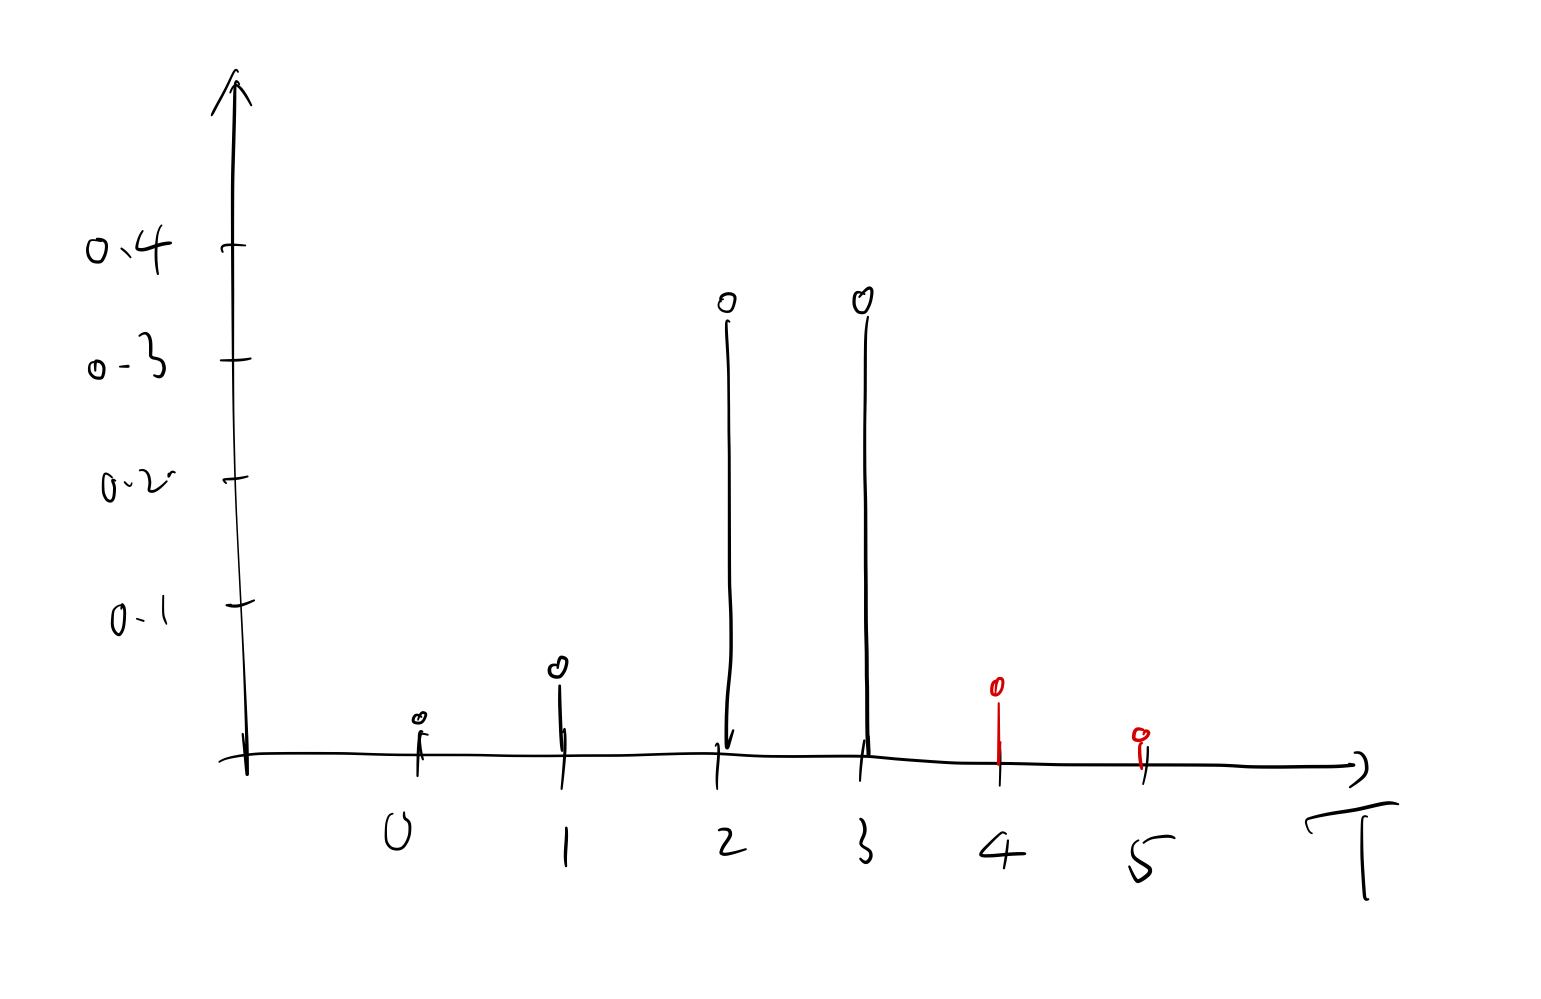
\includegraphics[width=0.7\textwidth]{figures/06-Hypothesis_testing/null_dist_binom.jpeg}
    %     \caption{猜拳實驗假說檢定的虛無分佈}
    %     \label{fig:}
    % \end{figure}

    % \begin{custom}{思考}
    %    如果把顯著水準提高,拒絕域應該會變寬或是變窄?
    % \end{custom}
    
    % \begin{table}[htbp]
    %     \begin{center}
    %         \begin{tabular}{ccccc}
    %             \toprule
    %             虛無假說($H_0$) & 對立假說($H_1$) & 檢定統計量 & $p$ 值 & 拒絕區\\
    %         \end{tabular}
    %         \caption{母體為常態分布且變異數未知的母體平均檢定\label{tab:}}
    %     \end{center}
    % \end{table}
    
    \bigskip 
    
    \begin{docexam}{(104-1醫學(一))}
        某研究為分析降血壓藥的效果,採用病例對照設計(case-control study),欲分析病例對照兩組樣本服降血壓藥3個月前後測量之血壓值差異是否有明顯不同,研究者應該使用何種統計方法最合適?

        (A) 配對 t 檢定 (Paired t-test)

        (B) 單一樣本 Z 檢定 (One sample Z-test)

        (C) Pearson 卡方檢定 (Pearson Chi-square test)

        (D) 獨立樣本 $t$ 檢定 (Independent t-test)
    \end{docexam}
    
    \begin{docexam}{(106-2醫學(二))}
        某研究者想檢定新藥是否有降血壓效果,對20隻大鼠在餵食新藥前後分別測量血壓值,對於兩次血壓測量值的比較,下列統計分析方法何者最恰當?

        (A) 線性回歸 (Linear regression)

        (B) 獨立樣本 $t$ 檢定 (Independent sample t-test)

        (C) 配對 t 檢定 (Paired t-test)

        (D) 列聯表分析 (Contingency table)
    \end{docexam}
    
    \begin{docexam}{(105-1醫學(一))}
        比較兩組病人某項檢驗數值的平均值(mean)是否有差異,可使用下列何種統計方法?

        (A) 卡方檢定 (Chi-square test)

        (B) $t$ 檢定 (Student's t test)

        (C) 曼惠特尼檢定 (Mann-Whitney test)

        (D) 符號檢定 (Sign test)
    \end{docexam}
    
    \begin{docexam}{(102-2醫學(一))}
        有關檢定兩個母群體平均值是否不同,統計推論可能會犯的錯誤型態及檢力 (power),下列何者錯誤?

        (A) 增加樣本數可以增加 power

        (B) 虛無假說為真時,作出推翻虛無假說的決定就犯 Type I error

        (C) 對立假說為真時,作出推翻虛無假說的決定的機率就是 power

        (D) 兩個母群體的平均值愈接近,power 就愈大
    \end{docexam}
    
    \begin{docexam}{(102-2醫學(一))}
        針對交通意外事故死亡者調查,從這些死亡者的左股動脈和左冠狀動脈各抽取血液樣本,以測量酒精濃度,總共抽取 25 個意外事故的死亡者。研究者的問題是「左股動脈的血液平均酒精濃度是否顯著不同於左冠狀動脈的血液平均酒精濃度?」你將採用何種統計方法檢定上述資料?

        (A) 獨立 $t$ 檢定

        (B) 卡方檢定

        (C) 配對 $t$ 檢定

        (D) 麥內瑪檢定 (McNemar's test)
    \end{docexam}
    
    \begin{docexam}{(101-2醫學(一))}
        有研究者報導其臨床試驗結果,實驗組的受試者感染率為 10\%,安慰劑組感染率為 13\%,兩組感染率差異的 95\% 信賴區間為 -2.6\% 至 8.6\%,下列敘述何者正確?        

        (A) 兩組的差異達統計顯著

        (B) 兩組的差異未達統計顯著

        (C) 應該採用變異數分析

        (D) 應該採用 $t$ 檢定
    \end{docexam}
    
    \begin{docexam}{(100-1醫學(一))}
        有一個研究探討某一藥物對於尿液鈣離子的排泄效應,有 9 位受試者被隨機選出,口服 0.5 毫克的藥物,在服用藥物 6 小時候收集這些人的尿液。另隨機抽取 16 位受試者,這些人不服用藥物,同樣在被隨機選出後 6 個小時收集這些人的尿液。研究者的問題是「這兩群人排泄的尿液鈣離子濃度是否顯著不同?」你將採用何種統計方法檢定上述資料?

        (A) 兩個樣本 $t$ 檢定

        (B) 卡方檢定

        (C) 配對 $t$ 檢定

        (D) 麥內瑪檢定 (McNemar's test)
    \end{docexam}
    
    \begin{docexam}{(110-1醫學(二))}
        如果想要比較年輕人與老年人的流感罹患率,王醫師隨機收集 $100$ 位年輕人與 $100$ 位老年人民眾,詢問其過去一個月是否罹患流感,其中有 $42$ 位年輕人及 $22$ 位老年人回答有,因此估計年輕人流感罹患率為 $0.42$,老年人流感罹患率為 $0.22$。下列何者最不恰當?

        (A) 王醫師的隨機抽樣必須排除有可能互相傳染的樣本,才能得到這些估計值

        (B) 王醫師的估計值 $0.42$,必須假設每個年輕人得流感的機率都是一樣且互相獨立,才能成立

        (C) 王醫師的老年人樣本如果源自 $1000$ 床的老人安養中心的隨機抽樣,則可能因為群聚效應,不宜視為獨立樣本

        (D) 王醫師可以合併樣本,利用 $200$ 人當中有 $42+22=64$ 位得到流感,來估計人口中得流感的機率為 $0.32$
    \end{docexam}


\chapter{相關性與線性回歸}

    我們在前面的章節中暸解了如何描述一個變數的特性,包含它的中心位置(如平均值、中位數)以及分散程度(如標準差、四分位差)。我們還可以利用信賴區間與假說檢定來對變數的母體平均作進一步的推論。在實務上,除了針對單一變數進行統計推論外,我們常也對兩個變數或多個變數之間的關係有興趣。例如:年齡越大,低密度膽固醇的平均值是否也隨之增高?每日平均鹽攝取量越高,脈壓的平均值是否也會隨之增高?要探討兩個變數之間的關係,我們就需要了解如何描述兩個變數的相關性(尤其是線性相關性),並且針對這個相關性的有無或強度進行統計推論。而後,我們還能進一步用線性回歸來對線性相關性做更細緻的描述及討論,並演示如何用簡單線性回歸建構出前面幾章提到的雙樣本 $t$ 檢定。最後,我們會討論當解釋變數有兩個以上時,如何利用多重線性回歸建模,以及模型參數的解釋。
    
    \begin{introduction}[第 \thechapter 章學習目標]
        \item 了解共變數與相關係數的定義,以及針對相關係數進行檢定
        \item 簡單線性回歸模型的建構以及參數解釋
        \item 簡單線性回歸的參數估計與統計推論
        \item 簡單線性回歸的模型解釋力與相關係數的關係
        \item 簡單線性回歸與雙樣本 $t$ 檢定的連結
        \item 多重線性回歸的參數解釋與模型選擇
        \item 了解變異數分析的目的及結果判讀
    \end{introduction}

\section{兩個變數的線性相關性}
    描述兩個變數相關性的方法,最簡單的方法是畫出\textit{散佈圖} (scatterplot)。例如圖\ref{fig:scatterplot}中,左上角 $X$ 與 $Y$ 之間沒有明顯的關係,因此我們稱 $X$ 與 $Y$ \textit{不相關} (uncorrelated)。右上角隨著 $X$ 的取值增大,$Y$ 的取值也跟著增大,而且可以隱約看出兩者之間的關係可以用圖中由左下到右上的藍色虛直線描述,因此我們稱 $X$ 與 $Y$ 呈現 \textit{正相關} (positively correlated)。左下角則是隨著 $X$ 的取值增大,$Y$ 的取值跟著減小,兩者之間的關係可以用圖中由左上到右下的藍色虛直線描述,因此我們稱 $X$ 與 $Y$ 呈現 \textit{負相關} (negatively correlated)。右下角中,$Y$ 的取值明顯和 $X$ 有關:$X$ 取值 $10$ 附近時,$Y$ 鮮少取值在 $15$ 附近,反之則不然,因此 $X$ 的取值會影響到 $Y$ 的取值。但是 $X$ 和 $Y$ 之前沒有很明顯的線性關係,因此他們雖然相關,但沒有線性相關。

    \begin{figure}[htbp]
        \centering
        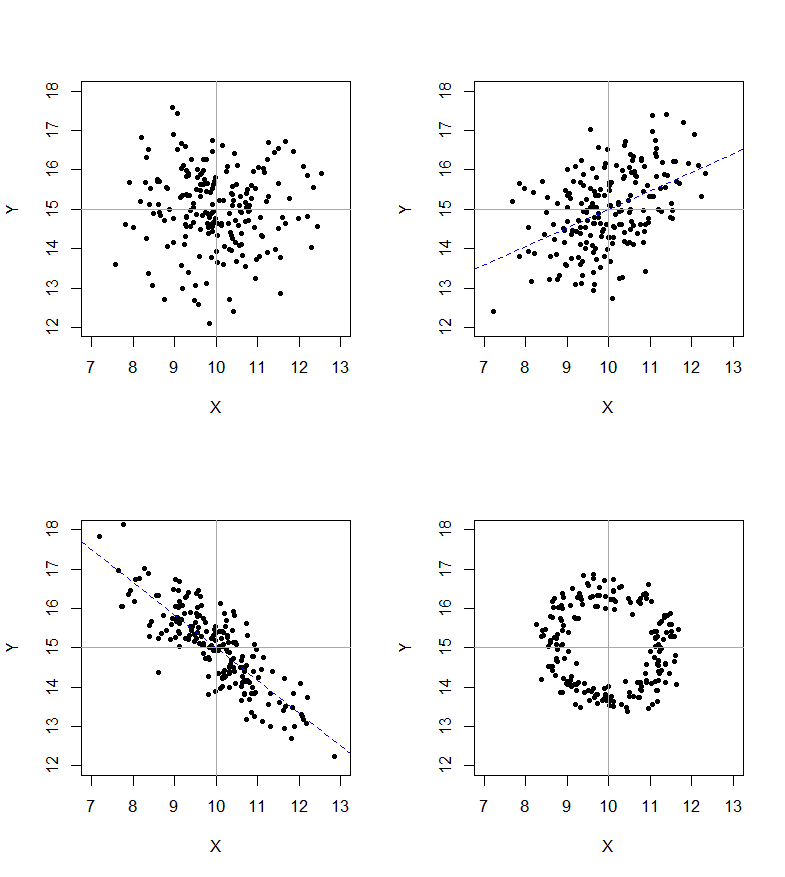
\includegraphics[width=0.7\textwidth]{figures/08-Correlation_linear_regression/scatterplot.png}
        \caption{散佈圖示例}
        \label{fig:scatterplot}
    \end{figure}

    為了量化線性相關的強弱,我們可以將圖\ref{fig:scatterplot}中的每個散佈圖以 $X$ 和 $Y$ 的平均值為基準分成四個象限。可以發現,右上圖呈現正相關,資料點也大多集中在第一和第三象限,也就是兩個變數經常同時大於平均值或同時小於平均值;相對地,左下圖呈現負相關,資料點也大多集中在第二和第四象限,也就是一個變數大於平均值時,另一個變數就常小於平均值,反之亦然;左上和右下兩個散佈圖的資料點則十分均勻地分布在四個象限中。根據這個觀察,我們可以建構以下關於 $X$ 和 $Y$ 的母體參數:
    \[cov(X,Y) = \EE[(X-\mu_X)(Y-\mu_Y)]\]
    其中 $\mu_X := \EE X$ 和 $\mu_Y := \EE Y$ 分別是 $X$ 和 $Y$ 的平均值。可以看到這個量是把 $X$ 和 $Y$ 都中心化(減去平均值)後相乘並取期望值,因此其為正代表 $X$ 和 $Y$ 經常同時大於平均值或同時小於平均值,即正相關;反之,其為負代表 $X$ 和 $Y$ 經常一個大於平均值、一個小於平均值,即負相關。由於這個量可以用來量化兩個隨機變數共同變化的狀況,因此被稱為 $X$ 和 $Y$ 的 \textit{共變異數} 或 \textit{共變數} (covariance)。當共變異數為正時,代表兩個變數呈現正相關;反之則為負相關;若共變異數恰好等於零,則兩個變數沒有線性相關。
    
    根據共變數的定義以及期望值的運算規則,我們可以推出一些以下的性質:
    \allowdisplaybreaks
    \begin{align*}
        cov(X,X) &= \EE[(X - \mu_X)^2] \\
        &= var(X)\\
        cov(X,Y+Z) &= \EE[(X - \EE X)((Y+Z) - \EE(Y+Z))] \\
        &= \EE[(X - \EE X)((Y+Z) - (\EE Y + \EE Z))] \\
        &= \EE[(X - \EE X)((Y-\EE Y) + (Z - \EE Z))] \\
        &= \EE[(X - \EE X)(Y-\EE Y)] + \EE[(X - \EE X)(Z - \EE Z))]\\
        &= cov(X,Y) + cov(X,Z)\\
        cov(aX,bY) &= \EE[(aX-\EE(aX))(bY-\EE(bY))]\\
        &= \EE[(aX-a\EE X)(bY-b \EE Y)]\\
        &= ab \cdot \EE[(X-\EE X)(Y- \EE Y)]\\
        &= ab \cdot cov(X,Y)
    \end{align*}
    第一個性質說明,隨機變數自己和自己的共變異數,等於其變異數。第二個性質顯示共變異數具有分配律。第三個性質則暗示共變異數的數值大小和 $X$ 及 $Y$ 的測量尺度有關:如果原本以公分測量身高、公斤測量體重得到的共變異數為 $4$(公分-公斤),那麼改用公尺測量身高時,身高的數值會變為原本的 $\frac{1}{100}$,而共變異數也會同時變成 $4 \cdot \frac{1}{100} = 0.04$ (公尺-公斤)。換言之,如果使用共變異數來量化身高和體重的線性相關,雖然正負號總會是正的,但其數值大小會隨著測量的單位而變化,而身高和體重的相關性顯然不會因為測量單位不同而有所不同。因此,共變異數不具有尺度不變性 (scale invariance),而非量化線性相關性的良好選擇。

    為了讓相關性的度量不受測量單位所影響,我們可以將中心化的隨機變數用其標準差\textit{標準化}(standardize)後再行相乘,也就是:
    \[\rho_{XY} = \EE\Big[\Big(\frac{X - \mu_X}{\sigma_X}\Big)\Big(\frac{Y - \mu_Y}{\sigma_Y}\Big)\Big] = \frac{cov(X,Y)}{\sigma_X \sigma_Y}\]
    其中 $\sigma_X$ 和 $\sigma_Y$ 為 $X$ 和 $Y$ 的標準差。此時,若 $X$ 因更改測量單位而數值變成 $a$ 倍,則 $X$、$\mu_X$ 和 $\sigma_X$ 均會同時變為 $a$ 倍,使倍數互相抵銷而 $\rho_{XY}$ 不變。這個用以兩個變數相關性的參數,其概念起先由統計學家 Francis Galton 提出,而後其門生 Karl Pearson 詳細推導其統計性質,因而被稱為\textit{皮爾森相關係數} (Pearson correlation coefficient) 或 \textit{皮爾森積差相關係數} (Pearson product-moment correlation coefficient)。皮爾森相關係數除了有我們前面提到的尺度不變性外,根據其定義還能推導出\textbf{其取值範圍為 $-1$ 到 $1$}。其中取值為 $1$ 或 $-1$ 時代表兩個隨機變數互為線性關係(例如 $X = 2Y+3$ 或 $X = -0.3Y-5$),若畫成散佈圖則資料點會呈現完美的直線,此時稱兩個隨機變數為\textit{完全相關} (perfectly correlated)。取值靠近 $1$(或 $-1$)時稱為高度相關,取值靠近 $0$ 時稱為低度相關,取值等於 $0$ 時稱為無線性相關。
    
    由於 $\rho_{XY}$ 是一個母體參數,我們通常仍需要用樣本來估計之,以利進一步對其作統計推論。分母的 $\sigma_X$ 和 $\sigma_Y$ 可以用樣本標準差 $s_X$ 和 $s_Y$ 來估計,分子的共變異數則利用樣本共變異數來估計:
    \[\widehat{cov}(X,Y) = \frac{1}{n-1}\sum_i (X_i - \bar{X})(Y_i - \bar{Y})\]
    其中 $n$ 為樣本數,$\bar{X}$ 和 $\bar{Y}$ 為 $X$ 和 $Y$ 的樣本平均數。這裡分母除以 $n-1$ 的理由和樣本變異數相同,是為了讓樣本共變異數成為母體共變異數的不偏估計量。最終的估計值可以寫為
    \[r_{XY} = \frac{\widehat{cov}(X,Y)}{s_X s_Y} = \frac{\sum_i (X_i - \bar{X})(Y_i - \bar{Y})}{\sqrt{\sum_i (X_i - \bar{X})^2}\sqrt{\sum_i (Y_i - \bar{Y})^2}}\]
    有了 $r_{XY}$ 這個估計值後,除了根據估計值判斷兩個變數的線性相關程度外,也可以針對 $\rho_{XY}$ 進行統計推論。由於 $r_{XY}$ 的抽樣分布通常較為偏斜(尤以 $\rho_{XY}$ 較接近 $-1$ 或 $1$ 時為甚),在進行統計推論前,一般會先對相關係數進行如下的轉換:
    \[z = \frac{1}{2}\ln\Big(\frac{1+r_{XY}}{1-r_{XY}}\Big)\]
    此時假設 $X$ 和 $Y$ 均服從常態分布,則 $z$ 的抽樣分布可用常態分布近似如下:
    \[z \sim \NN\Big(\frac{1}{2}\ln\Big(\frac{1+\rho_{XY}}{1-\rho_{XY}}\Big), \frac{1}{n-3}\Big)\]
    這個轉換方法與近似抽樣分布由統計學家 Ronald Fisher 所提出,因此也被稱為\textit{費雪轉換} (Fisher transformation)。而後即可用此抽樣分布導出 $z$ 在假說檢定中的虛無分佈,或是建構 $\rho_{XY}$ 的信賴區間。其中最常用的是藉由檢定 $\rho_{XY}$ 是否等於零,以推論 $X$ 和 $Y$ 是否有線性相關。然而需要注意的是,兩個變數之間有相關,只代表在資料中他們有朝同一個方向(或相反方向)變動的趨勢,並不代表他們之間必然有因果關係。例如,如果拿每個月的冰淇淋銷量與海邊溺水人數計算相關係數,將會發現有顯著的正相關,但這不代表食用冰淇淋會增加溺水的風險,而只是因為天氣炎熱時同時會讓冰淇淋銷量增加與海邊戲水的人數增加(進而使溺水人數增加),造成兩者數據的同向變化。因此,我們需要利用實驗設計(例如隨機對照實驗)或是排除其他造成相關性的非因果因素,才能將資料中呈現的相關性解釋為因果關係。我們在後續章節談到多重線性回歸時,會再深入探討這個議題,但截至目前為止,讀者應該謹記\textbf{相關不代表因果} (Correlation does not imply causation)。

    \bigskip

    \begin{custom}{練習}
        某研究發現,入住外科加護病房患者的初始體溫(以攝氏度量測)與血清發炎指標 CRP 濃度(以 mg/dL 為單位)之皮爾森相關係數為 0.74。若體溫改為華氏度量測,該相關係數將變為多少?
    \end{custom}

    \bigskip

    \begin{custom}{練習}
        某研究欲了解尿液中的 A 化合物濃度與第二型糖尿病患者的糖化血色素是否有相關。搜集了 103 名病患並計算兩者之相關係數後得到估計值及其 95\% 信賴區間為 0.150 (-0.045, 0.334)。在設定顯著水準為 0.05 下,請根據研究問題進行假說檢定並說明結論。
    \end{custom}

\section{簡單線性回歸}

    我們前一節提到可以用相關係數來描述兩個變數之間的線性關係。舉例而言,如果清華大學學生的身高與體重的相關係數為 0.8,呈現頗強的正相關。這代表身高較高的學生體重也相對較高。然而,這個相關係數只告訴我們兩個變數間呈現正向的線性關係,而不能告訴我們隨著身高的增加,體重\textbf{增加的幅度}為何。另外,我們也不能從相關係數來\textbf{預測}給定身高下,學生體重的預期值為何。由此看來,相關係數只給了我們兩個變數間線性關係的強度和方向,但是並沒有給我們該線性關係的全貌。

    \subsection{簡單線性回歸的模型與參數}
    
    為了瞭解兩個變數 $Y$ 與 $X$ 之間的線性關係,統計上採取的策略是先建立 $Y$ 和 $X$ 之間的線性模型,然後用資料估計模型的參數,並對這些參數來做推論。我們以圖 \ref{fig:SLR} 為例,散佈圖如左圖。假設體重變數記為 $Y$,身高變數記為 $X$,而且我們有興趣的是在身高 $X$ 變化下,體重 $Y$ 的預期變動。此時 $Y$ 稱為\textit{反應變數} (response variable) 或\textit{應變數} (dependent variable),而 $X$ 稱為\textit{解釋變數} (explanatory variable) 或\textit{自變數} (independent variable)。理想上,我們希望可以直接用一條直線 $Y = \beta_0 + \beta_1 X$ 來完全描述 $Y$ 和 $X$ 之間的關係,但大多數情況下兩個變數不會剛好呈現直線關係(除非兩者呈現完全相關)。因此,我們退而求其次,假設
    \[Y = \beta_0 + \beta_1 X + \varepsilon, \qquad \varepsilon \sim \NN(0, \sigma^2)\]
    其中 $\beta_0 + \beta_1 X$ 代表的是圖 \ref{fig:SLR} 左圖的黑色斜直線,也就是給定身高下,模型預期的體重。$\varepsilon$ 則是誤差項,代表實際值和預期值的差異,也就是每個觀察值黑點到斜直線的垂直距離。誤差項的來源可能來自測量誤差,但更多時候是起源於研究中未測量到的變數。例如,如果學生中有一群人偏高熱量飲食、一群人則篇低熱量飲食,我們分別以圖 \ref{fig:SLR}中間和右邊的子圖獨立標記這兩群人後可以發現,考量飲食熱量高低對體重的影響後,同一群飲食習慣者內部的誤差項就相對較小。誤差項的分佈方面,我們假設它們服從平均值為$0$,變異數為 $\sigma^2$ 的常態分布。注意到我們這裡假設不論 $X$ 是多少,誤差項的變異數皆為 $\sigma^2$,這個假設被稱為\textit{同質變異性} (homoscedasticity)。同質變異性的假設不見得在所有資料都成立,例如體重的變異性可能在身高較高的人較大,在身高較矮的人則較小,此時就需要使用較進階的統計方法來處理這類\textit{異質變異性} (heteroscedasticity) 的課題。在這個章解中,為了簡化流程,我們仍然保留同質變異性的假設。

    我們以下回顧整理簡單線性回歸所做的假設,其代表的英文字恰恰可以縮寫成「LINE」:
    \begin{itemize}
        \item 線性(\textbf{L}inearity):給定自變數 $X$ 下,應變數 $Y$ 的期望值和 $X$ 的取值呈線性關係。
        \item 獨立誤差(Error \textbf{I}ndependence):每個觀察值的誤差 $\epsilon_i$ 均互相獨立。
        \item 常態誤差(Error \textbf{N}ormality):每個觀察值的誤差 $\epsilon_i$ 均服從常態分佈。
        \item 同質變異性(Homoscedasticity, 或 Error \textbf{E}quivariance):每個觀察值的誤差 $\epsilon_i$ 變異數均等。
    \end{itemize}
    注意到我們只假設了\textbf{誤差}呈現常態,而對 $Y$ 和 $X$ 的分布並沒有進行限制。換言之,進行簡單線性回歸時,應變數和自變數\textit{不需要}遵從常態分佈。

    \begin{figure}[htbp]
        \centering
        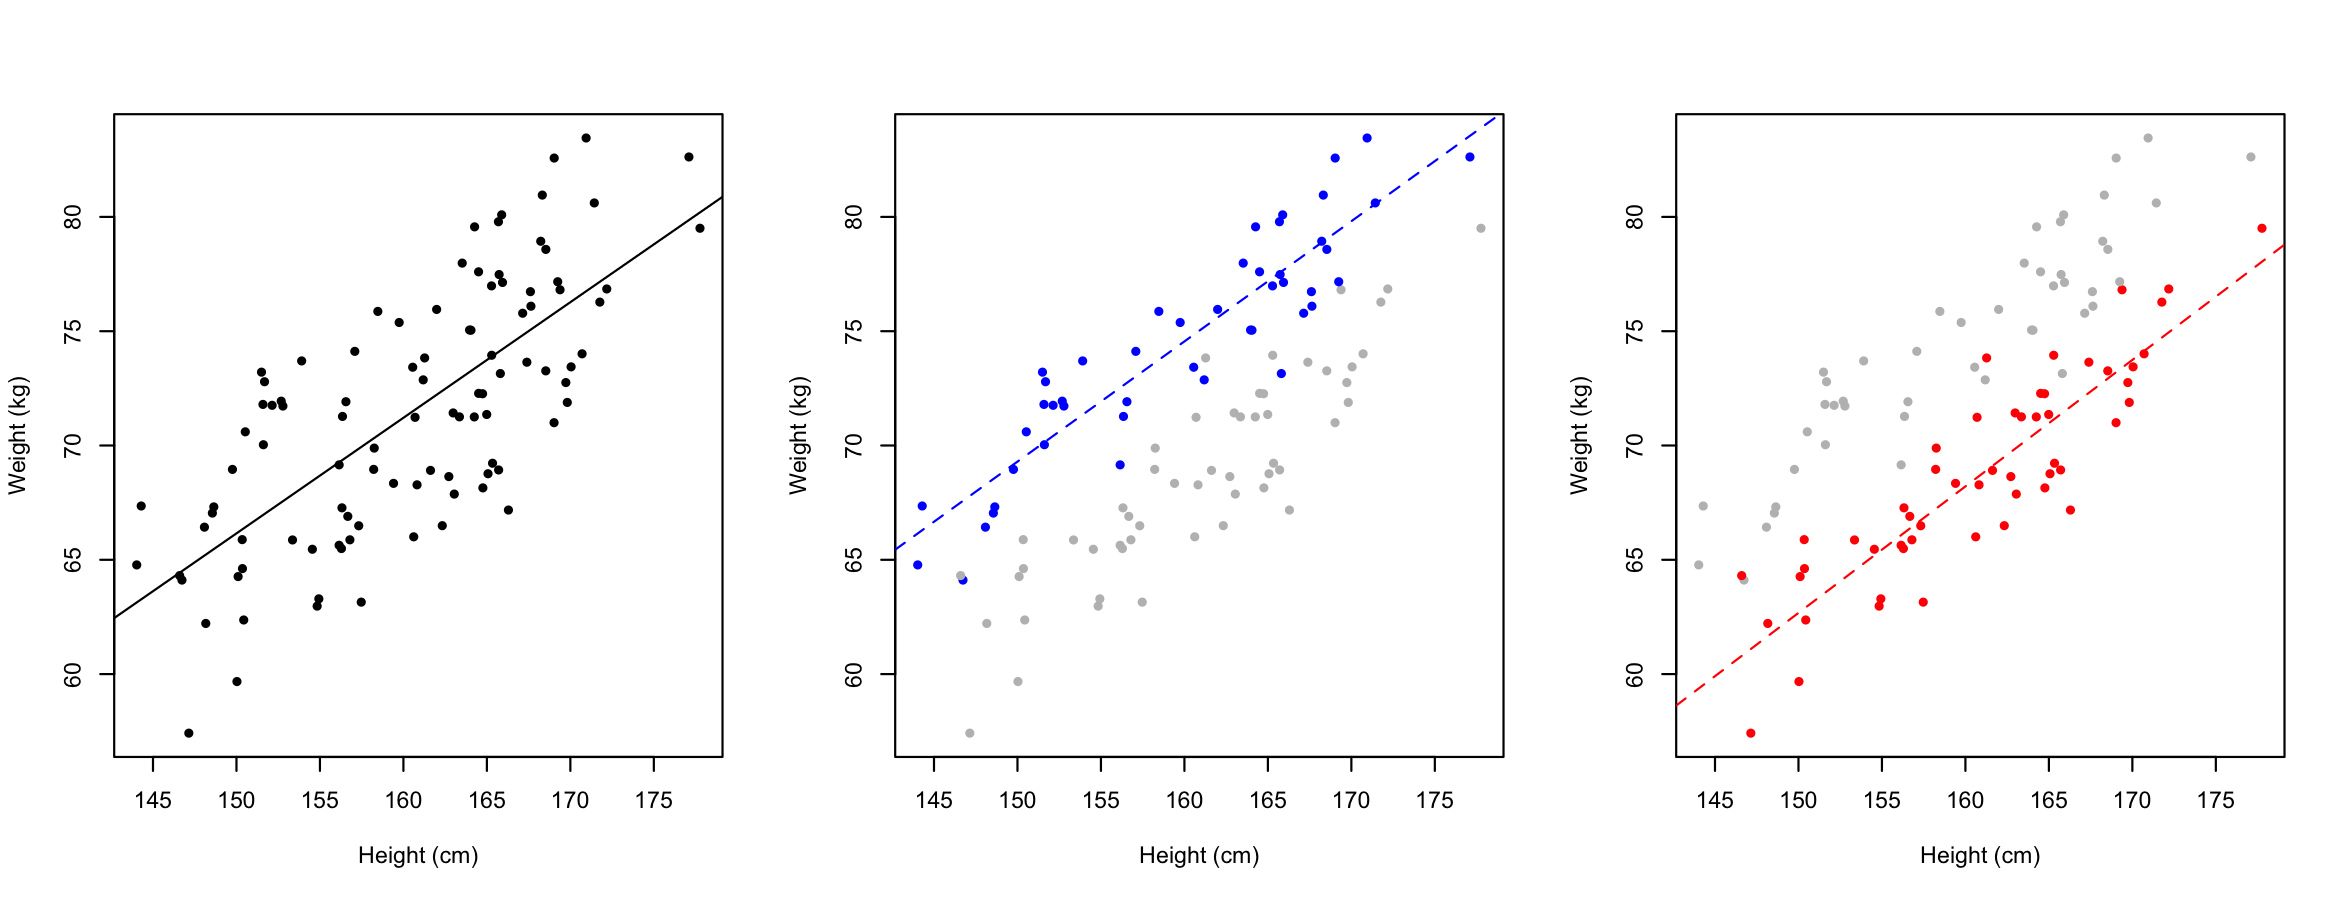
\includegraphics[width=\textwidth]{figures/08-Correlation_linear_regression/regression.png}
        \caption{簡單線性回歸的散佈圖}
        \label{fig:SLR}
    \end{figure}

    根據前述的簡單線性回歸模型,當我們已知一個學生的身高為 $x$ 公分,那麼他的實際體重會以 $\beta_0 + \beta_1 x$ 公斤為中心,加入一個上下變動的誤差項,且這個誤差項來自於變異數為 $\sigma^2$ 的常態分布。我們無法預測誤差項的值,但知道其期望值為零,因此我們預期該學生的身高\textbf{平均而言}為 $\beta_0 + \beta_1 x$ 公斤。準此,我們就能得出模型中兩個參數 $\beta_0, \beta_1$ 的白話解釋(這兩個係數又被稱為\textit{回歸係數} (regression coefficients))
    \begin{itemize}
        \item $\beta_0$:又被稱為\textit{截距} (intercept),代表解釋變數 $X$ 取值為 $0$ 時,反應變數 $Y$ 的平均值。
        \item $\beta_1$:又被稱為\textit{斜率} (slope),代表解釋變數 $X$ 每增加 $1$ 單位時,反應變數 $Y$ 的平均值的增加量。
    \end{itemize}
    可以看出,通常我們有興趣的是斜率 $\beta_1$:當 $\beta_1 \ne 0$ 時,代表解釋變數 $X$ 的變動對於反應變數 $Y$ 有線性影響。至於截距 $\beta_0$ 的數值我們通常不太關心,這個數值甚或不符合現實情境。例如在上述的例子中,$\beta_0$ 代表一個 $0$ 公分的學生預期的平均體重。這在現實上沒有任何實用意義,只是回歸模型外插至 $X=0$ 用以建模的參數而已。

    \subsection{簡單線性回歸的參數估計及推論}

    建立線性回歸模型後,我們的目的是要利用資料估計模型的參數並進行推論。假設我們把第 $i$ 個觀察值的反應變數和解釋變數數值記為 $Y_i$ 和 $X_i$。另外,我們將斜率的估計值寫為 $\hat{\beta}_1$、截距的估計值寫為 $\hat{\beta}_0$,那麼對於第 $i$ 個觀察值,我們預期其反應變數的平均值為 $\hat{\beta}_0 + \hat{\beta}_1 X_i$,而其反應變數的實際數值為 $Y_i$。這兩者之間的差 $e_i = Y_i - (\hat{\beta}_0 + \hat{\beta}_1 X_i)$ 被稱為 \textit{殘差} (residual)。殘差的大小越小,代表我們的估計越準,因此我們目標應該要將總體的殘差大小最小化。在統計中,為了計算方便,我們最小化的是每個觀察值的殘差平方的總和,如下所示。這個方法也被稱為\textit{最小平方法} (method of least squares):
    \[L = \sum_i e_i^2 = \sum_i  [Y_i - (\hat{\beta}_0 + \hat{\beta}_1 X_i)]^2\]
    利用簡單的微分(或是二次多項式求極值的方法)可得,能夠將 $L$ 最小化的 $\hat{\beta}_1$ 和 $\hat{\beta}_0$ 為
    \begin{align*}
        \hat{\beta}_1 &= \frac{\sum_i (X_i - \bar{X})(Y_i - \bar{Y})}{\sum_i (X_i-\bar{X})^2} = \frac{\widehat{cov}(X,Y)}{s_X^2} = r_{XY}\frac{s_Y}{s_X}\\
        \hat{\beta}_0 &= \bar{Y} - \hat{\beta_1}\bar{X}
    \end{align*}
    注意到 $\hat{\beta}_1$ 恰好等於 $r_{XY}$ 乘上一個恆正的 $s_Y / s_X$,因此他們的正負號是同向的。這很符合直覺,因為當兩個變數呈現正相關時,我們預期其中一個變數增加時,另一個變數也會同時增加,因此回歸斜率為正;反之當呈現負相關時,兩個變數的增減趨勢相反,所以回歸斜率應為負。為了進一步了解這組估計值的好壞,我們可以計算 $\hat{\beta}_1$ 和 $\hat{\beta}_0$ 的期望值和變異數,並得到
    \begin{align*}
        \EE\hat{\beta}_1 = \beta_1 \quad &; \quad \EE\hat{\beta}_0 = \beta_0\\
        var(\hat{\beta}_1) = \frac{\sigma^2}{(n-1)s_X^2} \quad &; \quad var(\hat{\beta}_0) = \sigma^2\Big(\frac{1}{n} + \frac{\bar{X}^2}{(n-1)s_X^2}\Big)
    \end{align*}
    首先我們可以看到這兩個估計值都是\textbf{不偏}的,也就是說它們的期望值都恰好等於他們要估計的母體參數 $\beta_1$ 和 $\beta_0$。另外關於估計值變異數的部分,我們可以分成幾個影響因子來看:
    \begin{itemize}
        \item 誤差的母體變異數 $\sigma^2$:由於誤差代表資料中無法被回歸模型解釋的部分,因此誤差變異數越大,代表資料中能用來推論回歸模型的資訊越少。因此,兩個回歸係數的估計值變異數都正比於誤差變異數,代表資料資訊越少,回歸係數估計值的準確度越低。
        \item 樣本數 $n$:樣本數增大,資料的資訊也增加,因此估計值變異數均會變小。
        \item 解釋變數的樣本變異數 $s_X^2$:當解釋變數變異數變小,代表資料中解釋變數的跨度較小,此時只要資料稍有變動,對於斜率的估計就會變化得很劇烈。讀者可以把回歸線想像成一根擀麵棍:當解釋變數跨度很大時,就像用雙手十隻手指分散地握住桿麵棍,即便其中一隻手指頭出力,桿麵棍也不會明顯地歪斜。相對地,解釋變數跨度很小時,就像雙手的手指擠在桿麵棍的中央,此時只要其中一根手指稍微出力,其他手指很難抗衡其變化,桿麵棍就會歪斜。
    \end{itemize}
    取得回歸係數的估計值後,注意到 $\hat{\beta}_1$ 和 $\hat{\beta}_0$ 的變異數都含有 $\sigma^2$,但 $\sigma^2$ 目前未知仍待估計。根據模型的假設,第 $i$ 個觀察值的誤差 $\varepsilon_i$ 可以移項寫成
    \[\varepsilon_i = Y_i - (\beta_0 + \beta_1 X_i) \sim \NN(0, \sigma^2)\]
    雖然我們不知道實際的誤差$\varepsilon_i$,但我們可以用殘差 $e_i = Y_i - (\hat{\beta}_0 + \hat{\beta}_1 X_i)$ 來估計誤差 $\varepsilon_i$,進而用殘差的「樣本變異數」來估計誤差的母體變異數 $\sigma^2$
    \[\hat{\sigma}^2 = \frac{1}{n-2}\sum_i e_i^2 = \frac{1}{n-2}\sum_i [Y_i - (\hat{\beta}_0 + \hat{\beta}_1 X_i)]^2\]
    這裡的樣本變異數和一般的樣本變異數公式有點差別:(1) 分母的部分不是 $n-1$ 而是 $n-2$,因為在計算時我們使用了 \textbf{2} 個估計的參數 $\hat{\beta}_1$ 和 $\hat{\beta}_0$,因此自由度要扣掉 $2$(一般的樣本變異數只使用了一個估計的參數 $\bar{X}$),(2) 平方和的部分 $e_i$ 沒有減去樣本平均,因為我們已知誤差的期望值為 $0$。取得誤差變異數的估計值 $\hat{\sigma}^2$ 後,我們就可以用資料估計出回歸係數估計值的變異數如下:
    \[\widehat{var}(\hat{\beta}_1) = \frac{\widehat{\sigma}^2}{(n-1)s_X^2} \quad ; \quad \widehat{var}(\hat{\beta}_0) = \hat{\sigma}^2\Big(\frac{1}{n} + \frac{\bar{X}^2}{(n-1)s_X^2}\Big)\]
    我們更常報告的是標準誤,也就是將變異數估計值開根號:
    \[\widehat{se}(\hat{\beta}_1) = \sqrt{\frac{\widehat{\sigma}^2}{(n-1)s_X^2}} \quad ; \quad \widehat{se}(\hat{\beta}_0) = \sqrt{\hat{\sigma}^2\Big(\frac{1}{n} + \frac{\bar{X}^2}{(n-1)s_X^2}\Big)}\]

    取得回歸係數的估計值以及其變異數後,我們就能對回歸係數進行假說檢定或是建立信賴區間。此處我們需要借助 $t$ 分布,並且有:
    \[\frac{\hat{\beta}_1-\beta_1}{\widehat{se}(\hat{\beta}_1)} \sim t_{n-2} \quad ; \quad \frac{\hat{\beta}_0-\beta_0}{\widehat{se}(\hat{\beta}_0)} \sim t_{n-2}\]
    此處 $t$ 分布的自由度為 $n-2$,同樣是因為計算分母的標準誤估計值時使用了兩個參數估計值。同理於前幾章的 $t$ 檢定,如果要進行顯著水準設定為 $\alpha$、假說為 $H_0: \beta_1 = 0;\; H_1: \beta_1 \ne 0$ 的雙尾檢定,則可計算 $t$ 檢定統計量(虛無假說下 $\beta_1 = 0$):
    \[t = \frac{\hat{\beta}_1}{\widehat{se}(\hat{\beta}_1)}\]
    該檢定的 $p$ 值即為 $2\times\PP(t_{n-2} \ge |t|)$,檢定統計量的拒絕區則為 $|t| \ge t_{n-2, \alpha/2}$。相對地,如果要建構 $\beta_1$ 的 $(1-\alpha)\times 100\%$ 雙尾信賴區間,則為:
    \[\Big(\hat{\beta}_1 - t_{n-2, \alpha/2}\widehat{se}(\hat{\beta}_1), \hat{\beta}_1 + t_{n-2, \alpha/2}\widehat{se}(\hat{\beta}_1)\Big)\]
    關於 $\beta_0$ 的假說檢定和信賴區間建構和 $\beta_1$ 相同,只是如同我們之前所說,大多數的時候我們對截距的推論不感興趣。事實上,一般在研究中甚至不會報告截距的估計值、信賴區間以及檢定結果。

    在簡單線性回歸中,我們還可以探討一個特例:如果自變數 $X$ 為二元變項且取值為 $0$ 或 $1$,代表觀察值可以被分成兩組,一組為 $X=0$、一組為 $X=1$。根據簡單線性回歸的模型假設:
    \[Y = \left\{\begin{array}{lr}
        \beta_0 + \varepsilon, & X = 0\\
        \beta_0 + \beta_1 + \epsilon, & X = 1
    \end{array}, \qquad \varepsilon \sim \NN(0, \sigma^2) \right.\]
    該假設顯示,$X=0$ 這一組的 $Y$ 母體平均為 $\beta_0$,$X=1$ 這一組的 $Y$ 母體平均為 $\beta_0 + \beta_1$,而且各組內部的觀察值都服從變異數為 $\sigma^2$ 的常態分布。因此,我們也可以把上述模型假設寫成:
    \[\left\{\begin{array}{lr}
        Y \sim \NN(\beta_0,\sigma^2), & X = 0\\
        Y \sim \NN(\beta_0 + \beta_1, \sigma^2), & X = 1
    \end{array} \right.\]
    可以發現,這組假設和「假設兩組母體變異數相等」的獨立樣本 $t$ 檢定所做的假設完全等價,而獨立樣本 $t$ 檢定之檢定標的是兩組母體平均的差,恰好就是 $\beta_1$。因此,針對兩組獨立資料,進行獨立樣本 $t$ 檢定會等同於檢定「以組別編碼 $X=0,1$ 為自變數的線性回歸斜率」。

    \bigskip

    \begin{custom}{練習}
       某研究將 HIV 病患血液中「CD4$^+$ T 細胞的個數對數 (以 10 為底)」對「接受抗病毒治療與否(接受 = 1、未接受 = 0)」作簡單線性回歸,得到斜率估計值與雙尾 $95\%$ 信賴區間為 $0.301$ 及 $(0.176,0.426)$。請用白話說明該回歸模型之結果。
    \end{custom}

    \bigskip

    \begin{custom}{思考}
       如果將體重(公斤)對身高建立兩個線性回歸模型,一個模型的身高用公分作單位,另一個模型的身高用公尺作單位,得到結果如下:

       \medskip
       
       \begin{tabular}{cccccccc}
            \toprule
            \multirow{2}{*}{身高單位} & \multicolumn{3}{c}{斜率} && \multicolumn{3}{c}{截距} \\
            \cline{2-4}\cline{6-8}
            & 估計值 & 標準誤 & 雙尾 $p$ 值 && 估計值 & 標準誤 & 雙尾 $p$ 值\\
            \hline
            公分 & $\hat{\beta}_1$ & $\hat{s}_1$ & $p_1$ && $\hat{\beta}_0$ & $\hat{s}_0$ & $p_0$ \\  
            公尺 & $\hat{\beta}_1^*$ & $\hat{s}_1^*$ & $p_1^*$ && $\hat{\beta}_0^*$ & $\hat{s}_0^*$ & $p_0^*$ \\
            \bottomrule
       \end{tabular}

       \medskip

       \noindent 請問每個 column 的兩個數值(例如 $\hat{\beta}_1$ 和 $\hat{\beta}_1^*$)的關係為何?
    \end{custom}

    \bigskip

    \begin{custom}{思考}
       前面我們提到,回歸係數 $\beta_1$ 的意義為「解釋變數 $X$ 每增加一單位,反應變數 $Y$ 平均增加的單位數」。後來我們推導出,$\beta_1$ 的估計值 $\hat{\beta}_1$ 和相關係數 $\rho_{XY}$ 的估計值 $r_{XY}$ 的關係為 $\hat{\beta}_1 = r_{XY} \frac{s_Y}{s_X}$。事實上,$\beta_1$ 和 $\rho_{XY}$ 的亦有相似的關係:
       \[\beta_1 = \rho_{XY} \frac{\sigma_Y}{\sigma_X} \qquad \; \qquad \rho_{XY} = \beta_1 \frac{\sigma_X}{\sigma_Y}\]
       其中 $\sigma_Y, \sigma_X$ 分別為 $Y$ 和 $X$ 的母體標準差。根據這個定義, $\rho_{XY}$ 的解釋意義為何?由於 $\rho_{XY}$ 必定介於 $-1$ 與 $1$ 之間,讀者是否能想像 Francis Galton 當初在發展回歸理論時,為何要將它稱之為「回歸 (regression)」?
    \end{custom}
    
    \section{簡單線性回歸模型的模型配適度與模型診斷}

    在配適完線性回歸模型後,除了檢視回歸係數的估計值以及統計推論結果外,我們也常想知道配適出的模型是否能有效地預測反應變數。在線性回歸中,模型的解釋力常以「解釋的變異比例」來量化。我們可以再次回到圖\ref{fig:SLR}關於預測體重的散布圖,並考慮兩種可能的預測模型:僅有身高、以及同時有身高和飲食習慣。資料中體重的分布寬度大約是 20 公斤。當我們用身高去預測體重,每個人的體重扣掉預測值後(即殘差),分布寬度就減小到約 10 公斤。如果我們進一步同時用身高和飲食習慣來預測體重,殘差的分布寬度更減低到 5 公斤左右。我們可以看到,隨著模型的解釋力越來越好,殘差的變異性、也就是模型未能解釋的資料變異性越來越小。我們可以把上述的觀察用下面的式子具象化:
    \[\text{總變異}  = \text{模型解釋變異} + \text{殘差變異}\]
    在線性回歸中,我們會用各種\textit{平方和} (sum of squares)來描述上面三項變異:
    \begin{itemize}
        \item 總變異:\textit{總平方和}(total sum of squares, SST)$\sum_i (Y_i - \bar{Y})^2$,描述資料相對於總平均的偏差。
        \item 模型解釋變異:\textit{回歸平方和} (regression sum of squares, SSR)$\sum_i (\hat{Y}_i - \bar{Y})^2$,描述模型預測值 $\hat{Y}_i$相對於總平均的偏差。
        \item 殘差變異:\textit{殘差平方和}(residual (error) sum of squares, SSE)$\sum_i (Y_i - \hat{Y}_i)^2$,描述資料相對於預測值的偏差。
    \end{itemize}
    這些平方和的定義恰好可以滿足我們上面的式子:
    \[\underbrace{\sum_i (Y_i - \bar{Y})^2}_{SST} = \underbrace{\sum_i (\hat{Y}_i - \bar{Y})^2}_{SSR} + \underbrace{\sum_i (Y_i - \hat{Y}_i)^2}_{SSE}\]
    從這個式子可以看到,藉由配適模型得到預測值 $\hat{Y}$,可以將總變異(SST)分割為模型可解釋的變異(SSR)和模型不能解釋的變異(SSE)兩個部分。我們可以將模型的解釋力用 SSR 和 SST 的比值 SSR/SST、也就是\textbf{模型解釋的變異比例}來代表。這個值被稱為模型的\textit{決定係數} (coefficient of determination) $R^2$,其取值範圍為 $0$ 到 $1$(因 SSR 和 SSE 均非負),越靠近 $1$ 代表模型的解釋力越強。實際將 $R^2$ 的計算方法寫出來可以發現:
    \begin{align*}
        R^2 = \frac{SSR}{SST} &= \frac{\sum_i (\hat{Y}_i-\bar{Y})^2}{\sum_i (Y_i - \bar{Y})^2}\\
        &= \frac{\sum_i (\hat{\beta}_0 + \hat{\beta}_1 X_i -\bar{Y})^2}{\sum_i (Y_i - \bar{Y})^2}\\
        &= \frac{\sum_i (\bar{Y} - \hat{\beta}_1 \bar{X}+ \hat{\beta}_1 X_i -\bar{Y})^2}{\sum_i (Y_i - \bar{Y})^2}\\
        &= \hat{\beta}_1^2 \frac{\sum_i (X_i - \bar{X})^2}{\sum_i (Y_i - \bar{Y})^2}\\
        &= \Big(\frac{\sum_i (X_i-\bar{X})(Y_i-\bar{Y})}{\sum_i (X_i-\bar{X})^2}\Big)^2 \frac{\sum_i (X_i - \bar{X})^2}{\sum_i (Y_i - \bar{Y})^2} \\
        &= \frac{[\sum_i (X_i-\bar{X})(Y_i-\bar{Y})]^2}{\sum_i (X_i - \bar{X})^2\sum_i (Y_i - \bar{Y})^2} = r_{XY}^2
    \end{align*}
    因此,\textbf{簡單線性回歸的決定係數恰為皮爾森相關係數的平方}。皮爾森相關係數越靠近 $1$ 或 $-1$,代表兩個變數的線性相關程度越強,也代表配適簡單線性回歸時的模型解釋力越大。

    最後,在配適線性回歸模型時,我們做了四個重要的模型假設:線性、獨立誤差、常態誤差、同質變異性,而我們的統計推論正確與否也取決於這些模型假設是否正確。因此,在取信於模型的推論前,我們應該先確認模型的假設是否符合資料,這個程序被稱為\textit{模型診斷}(model diagnostics)。針對線性的假設部分,我們可以用散布圖來觀察兩個變數間的關係是否為線性,獨立誤差的部分則可以用資料搜集的過程來論證。不過常態誤差和同質變異性的假設,則因為是針對誤差而非資料的觀察值,我們必須利用殘差來做圖分析。圖\ref{fig:diagnostics}的左上、右上和左下三個圖是拿回歸的殘差對自變數 $X$ 作圖。殘差是誤差的估計值,而根據假設,誤差應該不論 $X$ 取值為何均服從相同變異數的常態分配。因此,正常的殘差圖應該如左上角,顯示殘差的分布不論 $X$ 取值為何均相同。右上角中,明顯看到殘差和 $X$ 仍然有一個曲線關係,這隱含著線性假設被違反。左下角中,殘差的變異數隨著 $X$ 增大而增大,隱含著同質變異性假設被違反。針對常態性假設,則可以繪製如右下角的常態百分位-百分位圖(或稱為\textit{常態 QQ 圖} (normal QQ plot))。在 QQ 圖中,每個點代表一個殘差值,橫坐標代表該殘差如果來自標準常態分布,根據其百分位數應該要取值多少(例如第 95 百分位應該取值 1.96):縱座標則為其實際取值。如果殘差的分布呈現常態,則這些殘差點應該會呈現一個左下到右上的直線,如右下圖的虛線所示。如果 QQ 圖顯示的圖形並非左下到右上的直線,則暗示著常態性假設有待商榷。前述模型診斷的結果如果顯示假設被違反,我們就需要回頭過來修改模型,例如進行非線性的回歸,或是套用更進階的統計方法來處理非常態或異質性的的誤差。

    \begin{figure}[htbp]
        \centering
        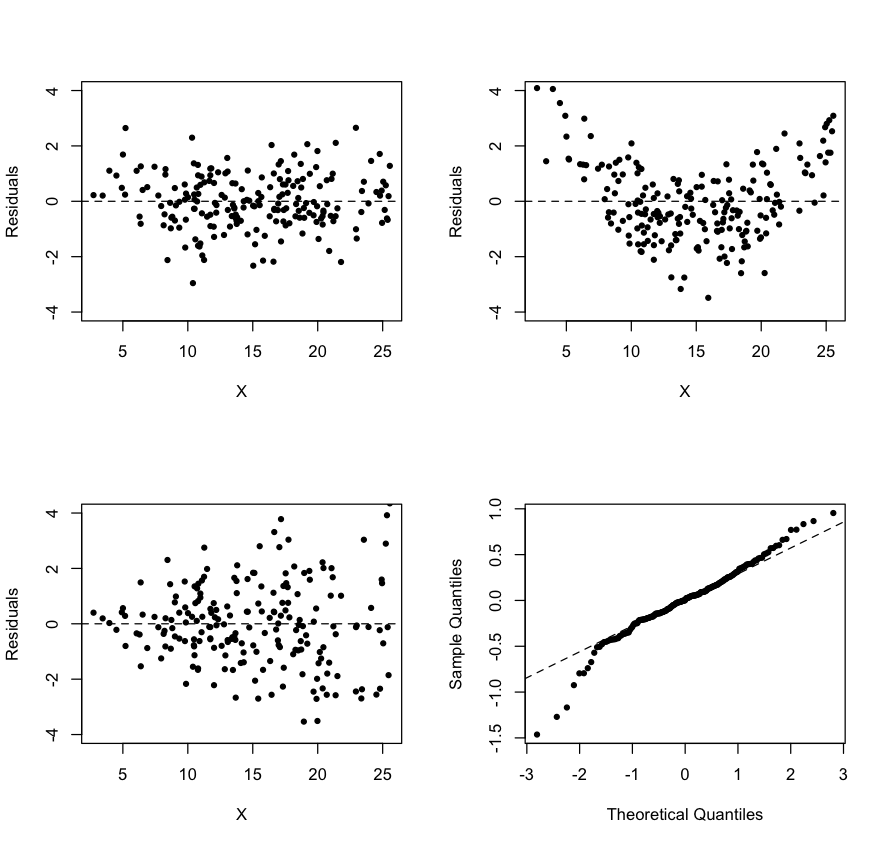
\includegraphics[width=\textwidth]{figures/08-Correlation_linear_regression/diagnostics.png}
        \caption{殘差圖與殘差 QQ 圖}
        \label{fig:diagnostics}
    \end{figure}

\section{多重線性回歸}
    在前面的章節中,我們使用簡單線性回歸來探討一個解釋變數 $X$ 和一個反應變數 $Y$ 的關係,但在生物醫學研究中,影響反應變數 $Y$ 的解釋變數往往不只一個。例如在圖\ref{fig:SLR}的例子中,一個人的體重可能與他的身高和飲食習慣均有關係。此時我們希望能在回歸模型中同時加入多個解釋變數,以增進模型對反應變數的解釋力。這種有多個解釋變數的線性模型被稱為\textit{多重線性回歸} (multiple linear regression),或簡稱多重回歸。

    假設我們有興趣的反應變數是 $Y$,另外有 $p$ 個用來解釋 $Y$ 的變數 $X_1, X_2, X_3,..., X_p$。多重線性回歸的模型假設如下:
    \[Y = \beta_0 + \beta_1 X_1 + \beta_2 X_2 + \cdots + \beta_p X_p + \varepsilon, \qquad \varepsilon \sim \NN(0,\sigma^2)\]
    可以看到多重線性回歸同樣繼承了簡單線性回歸的四個假設:(1) 線性:給定解釋變數下,$Y$ 的期望值是這些變數的線性組合 (2) 獨立誤差:每筆觀察值的誤差 $\varepsilon_i$ 均獨立 (3) 常態誤差:誤差均服從常態分布 (4) 同質變異性:誤差變異數不隨解釋變數取值而變化。
    
    上述多重線性回歸模型中,截距項 $\beta_0$ 的解釋意義和簡單線性回歸類似:當所有的解釋變數都取值為 $0$ 時,$Y$ 的平均值即為 $\beta_0$。至於其他回歸係數,例如 $\beta_1$ 的意義,則是在 \textit{控制其他解釋變數不變的情況下},$X_1$ 每增加 $1$ 單位時,$Y$ 平均值的變化。這裡之所以需要強調控制其他解釋變數不變,是因為各解釋變數經常會有相關性,因此其中一個解釋變數變動時,可能隱含了其他變數也會有預期下的變動。舉例來說,如果身高和體重均為解釋變數,那麼我們在想像一個身高較高的人時,其實也預期其體重也會較重。然而,身高的回歸係數說明的是,在\textbf{同樣體重}的情況下,身高每增加一單位,反應變數平均值的變化。

    \begin{figure}[htbp]
        \centering
        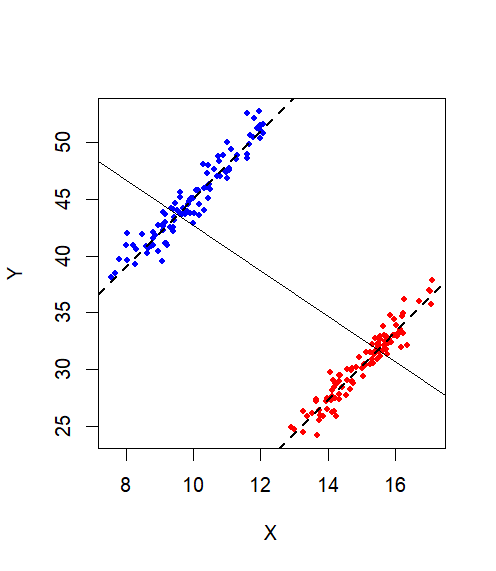
\includegraphics[width=0.5\textwidth]{figures/08-Correlation_linear_regression/confounding.png}
        \caption{多重回歸和簡單回歸結論不同的演示}
        \label{fig:confounding}
    \end{figure}
    
    多重回歸這個「控制其他解釋變數」的特性,甚至可能造成簡單回歸和多重回歸關於變數關係的方向結論不同。如圖\ref{fig:confounding}的散布圖所示,假設我們想知道變數 $X$ 與變數 $Y$ 的關係。直接將 $Y$ 對 $X$ 進行簡單回歸會得到黑色的回歸線。其斜率為負,亦即隨著 $X$ 的取值增加,$Y$ 的平均值會降低。然而,如果我們還知道每個觀察值可以分為紅色和藍色兩組,並把組別編碼為一個二元變數 $Z$ 後,將 $Y$ 對 $X$ 和 $Z$ 進行多重回歸,此時 $X$ 的回歸係數代表\textbf{控制顏色變數 $Z$ 不變的情況下},$X$ 每增加一單位,$Y$ 的平均增加量。從圖中可以看出,不論是控制顏色組別為藍色或紅色,$Y$ 的平均反而都是隨著 $X$ 增加而增加,和簡單回歸的結論不同。
    
    不過注意到,上面簡單回歸和多重回歸的結論雖然不同,但兩者\textbf{都是正確的}:如果僅從 $X$ 的數值想單方向地預測 $Y$,那麼較大的 $X$ 的確應該預測出較低的 $Y$。然而控制顏色組別 $Z$ 的影響後,$X$ 和 $Y$ 的關係就轉變為正向。這種新增解釋變數後造成回歸係數方向相反的現象也被統計學家稱為\textit{逆轉悖論} (reversal paradox)。

    多重線性回歸的回歸係數依然最常以最小平方法來估計,但計算的過程牽涉到矩陣運算,因此在這裡我們不會深入探討。獲得回歸係數的估計值 $\hat{\beta}_0, \hat{\beta}_1, \hat{\beta}_2, ... \hat{\beta}_p$後,即可依類似簡單線性回歸的方法計算各觀察值的殘差:
    \[e_i = Y_i - (\hat{\beta}_0 + \hat{\beta}_1 X_i + \hat{\beta}_2 X_2 + \cdots + \hat{\beta}_p X_p)\]
    而殘差的「樣本變異數」即為誤差變異數的估計值:
    \[\hat{\sigma}^2 = \frac{1}{n-p-1}\sum_i e_i^2\]
    注意到這裡的分母和簡單線性回歸不同,因為計算殘差時用到 $p+1$ 個回歸係數估計值,所以分母的地方要減去 $p+1$。得到誤差變異數的估計值後,即可再經過矩陣運算得到各回歸係數估計值 $\hat{\beta}_0, \hat{\beta}_1, \hat{\beta}_2, ... \hat{\beta}_p$ 的標準誤估計值 $\widehat{se}(\hat{\beta}_0), \widehat{se}(\hat{\beta}_1), \widehat{se}(\hat{\beta}_2), ..., \widehat{se}(\hat{\beta}_p)$。

    利用回歸係數的估計值及其標準誤的估計值,即可對各迴歸係數進行假說檢定或信賴區間的建構。我們同樣借助 $t$ 分布,並且有:
    \[\frac{\hat{\beta}_j - \beta_j}{\widehat{se}(\hat{\beta}_j)} \sim t_{n-p-1}, \qquad j = 0,1,2,...p\]
    此處 $t$ 分布的自由度為 $n-p-1$,因為計算分母的標準誤估計值時使用了 $p+1$ 個參數估計值。和簡單回歸同理,如果要進行顯著水準為 $\alpha$,檢定 $\beta_j$ 是否為 $0$ 的雙尾檢定,則可計算如下 $t$ 檢定統計量:
    \[t = \frac{\hat{\beta}_j}{\widehat{se}(\hat{\beta}_j)}\]
    該檢定的 $p$ 值為 $2\times\PP(t_{n-p-1} \ge |t|)$,檢定統計量的拒絕區則為 $|t| \ge t_{n-p-1, \alpha/2}$。當虛無假說被拒絕時,代表在控制其他解釋變數不變的情況下,解釋變數 $X_j$ 和 $Y$ 之間有顯著的線性關係。如果要建構 $\beta_j$ 的 $(1-\alpha)\times 100\%$ 雙尾信賴區間,則為:
    \[\Big(\hat{\beta}_j - t_{n-p-1, \alpha/2}\widehat{se}(\hat{\beta}_j), \hat{\beta}_j + t_{n-p-1, \alpha/2}\widehat{se}(\hat{\beta}_j)\Big)\]
    
\section{多重線性回歸的模型選擇}
    在多重線性回歸中,除了檢定其中一個回歸係數是否為 $0$ 外,有時候我們有興趣的命題是一群回歸係數是否同時為 $0$。例如(不失一般性地)我們想知道 $\beta_1, \beta_2, ..., \beta_q$ 是否同時為零,此時我們的假說可寫為:
    \[\left\{\begin{array}{l}
        H_0: \beta_1 = \beta_2 = \cdots = \beta_q = 0\\
        H_1: (\beta_1 \ne 0) \text{ or } (\beta_2 \ne 0) \text{ or } ... \text{ or } (\beta_q \ne 0)
    \end{array}\right.\]
    在虛無假說 $H_0$ 下,$\beta_1, \beta_2, ..., \beta_q$ 均為 $0$,意味著我們在配適多重線性回歸時,其實不用納入 $X_1, X_2, ..., X_q$,只要納入 $X_{q+1}, X_{q+2}, ..., X_p$ 即可。我們可以把這個比較限縮的模型稱為 $M_0$(意味著虛無假說下的模型),而將納入所有解釋變數的模型稱為 $M_1$(意味著對立假說下的模型),整理如下:
    \[\left\{\begin{array}{ll}
        M_0: Y = \beta_0  &+ \beta_{q+1} X_{q+1} + \beta_{q+2} X_{q+2} + \cdots + \beta_{p} X_{p} + \varepsilon\\
        M_1: Y = \beta_0 + \beta_1 X_1 + \beta_2 X_2 + \cdots  + \beta_q X_q &+ \beta_{q+1} X_{q+1} + \beta_{q+2} X_{q+2} + \cdots + \beta_{p} X_{p} + \varepsilon
    \end{array}\right.\]
    如果我們最後拒絕虛無假說,即表示 $M_0$ 忽略了一些有用的解釋變數,所以我們應該用 $M_1$ 來建模。如果我們無法拒絕虛無假說,那麼根據統計上\textit{奧卡姆剃刀} (Occam's razor)的原則,沒有證據顯示兩個模型配適度有差別時,傾向選擇較精簡的模型,因此我們就會選用 $M_0$ 來建模。
    
    在這裡,如果我們將兩個模型的總平方和 (SST)、回歸平方和 (SSR) 和殘差平方和 (SSE) 用圖示表示,會如圖\ref{fig:anova}所示:

    \begin{figure}[htbp]
        \centering
        \begin{tabular}{|c|c|c|c|c|}
            \cline{1-1}\cline{3-3}\cline{5-5}
            \multirow{8}{*}{$SST$} && \multirow{4}{*}{$SSR_0$} && \multirow{6}{*}{$SSR_1$}\\
             && &&  \\
             && &&  \\
             && &&  \\
            \cline{3-3}
             && \multirow{4}{*}{$SSE_0$} && \\
             && &&  \\
            \cline{5-5}
             && && \multirow{2}{*}{$SSE_1$} \\
             && &&  \\
            \cline{1-1}\cline{3-3}\cline{5-5}
            \multicolumn{1}{c}{}&\multicolumn{1}{c}{}& \multicolumn{1}{c}{$M_0$} &\multicolumn{1}{c}{}& \multicolumn{1}{c}{$M_1$} 
        \end{tabular}
        \caption{多重回歸模型比較之平方和分解}
        \label{fig:anova}
    \end{figure}

    圖\ref{fig:anova}中,$SSR_0$、$SSE_0$ 分別為限縮模型 $M_0$ 的回歸和殘差平方和; $SSR_1$、$SSE_1$ 分別為完整模型 $M_1$ 的回歸和殘差平方和。由於 $M_0$ 是 $M_1$ 限縮而來,$M_1$ 中只要把 $\beta_1$ 到 $\beta_q$ 都估計為 $0$,就可以得到和限縮模型 $M_0$ 一模一樣的模型,因此 $SSR_1 \ge SSR_0$。如果要用檢定證明 $M_1$ 優於 $M_0$,我們不能單純提出 $SSR_1 \ge SSR_0$,而是要呈現他們的差異「夠大」。

    統計學上可以證明出,在虛無假說下,$\frac{SSR_1-SSR_0}{q}$ 的期望值恰好等於誤差變異數 $\sigma^2$(其中分母的 $q$ 為兩個模型的參數個數差)。同時,由於 $SSE_1$ 即為 $M_1$ 模型算出的殘差平方和,根據前面關於多重回歸統計推論的結果,我們可以用 $\frac{SSE_1}{n-p-1}$ 來估計誤差變異數 $\sigma^2$。準此,我們將兩個在虛無假說下均能估計誤差變異數的統計量相除,建立出以下的檢定統計量並得出它的虛無分布:
    \[F = \frac{(SSR_1 - SSR_0)/q}{SSE_1/(n-p-1)} \sim F_{q, n-p-1}\]
    其中 $F_{q, n-p-1}$ 為一個新的分布,稱為 $F$ 分布;其具有兩個參數,分子自由度(此處為$q$)和分母自由度(此處為$n-p-1$)。在對立假說為真時,由於 $M_0$ 省略掉了有解釋能力的解釋變數,因此其配適度會劣於 $M_1$,造成 $SSR_0$ 遠低於 $SSR_1$,因此 $\frac{SSR_1-SSR_0}{q}$ 的期望值會高於 $\sigma^2$,使 $F$ 檢定統計量的數值偏大。因此本檢定的 $p$ 值須取右尾機率 $\PP(F_{q, n-p-1} \ge F)$,且顯著水準為 $\alpha$ 的拒絕區亦為右尾的 $F > F_{q, n-p-1, \alpha}$。此檢定被稱為模型比較的 \textit{$F$ 檢定} ($F$ test)。
    
    注意到這個檢定拒絕虛無假說時,我們僅能確定 $\beta_1, \beta_2, ... \beta_q$ \textbf{至少其中一個不為 $0$},但該檢定並不能告訴我們是哪幾個回歸係數顯著不為 $0$。如果需要深入探討哪幾個不為 $0$,則需進行前面統計推論提到的 $t$ 檢定再行定奪。

    % 跳過 Bonferroni

\section{變異數分析}
    前面的小節提到,若欲比較兩組獨立樣本的母體平均值,可以把組別編碼為取值為 $0$ 和 $1$ 的二元變數後,將觀察值對分組變數做簡單線性回歸並針對斜率進行檢定。這個檢定亦等價於「假設兩組母體變異數相等」的獨立樣本 $t$ 檢定。那麼,如果我們想比較三組以上獨立樣本的母體平均值,是否也可以用回歸的方式進行檢定呢?答案是肯定的。
    
    在回歸模型中,如果解釋變數中包含多元的類別變項,那麼我們\textbf{不能}直接將該類別變項編碼為 $0, 1, 2, 3,...$ 後直接代入模型,因為這將隱含這些組別之間的差異是等距的。舉例而言,假設有一個類別變項 $X$ 共有三個層次且被編碼為 $X = 0, 1, 2$。若直接將反應變數 $Y$ 對 $X$ 作簡單回歸並得到斜率為 $\beta_1$,則 $X=1$ 和 $X=0$ 兩組的 $Y$ 平均值差異和 $X=2$ 和 $X=1$ 兩組的 $Y$ 平均值差異均等於 $\beta_1$,但我們並不願做這個多餘的假設。
    
    為了避免上述的假設,一個最基礎常用的策略是利用\textit{虛擬變項} (dummy variables)(或稱\textit{獨熱編碼} (one-hot encoding))來編碼多元類別變項。當變項有 $k$ 個層次時,我們任選其中一個層次為\textit{對照} (reference) 層次,並新建 $k-1$ 個二元變項,其中每一個變項對應到一個非對照層次:若該觀察值隸屬於該層次則變項取值為 $1$,反之為 $0$。舉例來說,表\ref{tab:dummy_variable}左側為一個有 5 個層次,有關教育程度的類別變項:0 代表國中以下、1 代表高中(職)、2 代表大專、3 代表碩士、4代表博士。將該變項轉換為虛擬變項後如右側表所示。由於原變項有 5 個層次,最終被轉換為 4 個虛擬變項。這裡我們選擇把「國中以下」當成對照層次,因此建立出來的虛擬變項分別代表高中(職)、大專、碩士、博士。教育程度為這四個層次者,即分別在對應的虛擬變項取值為 1。教育程度為對照組的國中以下者,則在這些虛擬變項均取值為 0。

    \begin{table}[htbp]
        \begin{center}
            \begin{tabular}{ccccccc}
                \cline{1-1} \cline{4-7}
                教育程度($X$) &&& 教 - 高中 (職) ($X_1$) & 教 - 大專 ($X_2$) & 教 - 碩士 ($X_3$) & 教 - 博士 ($X_4$)\\
                \cline{1-1} \cline{4-7}
                1 &&& 1 & 0 & 0 & 0\\
                0 &&& 0 & 0 & 0 & 0\\
                1 &&& 1 & 0 & 0 & 0\\
                3 &&& 0 & 0 & 1 & 0\\
                4 &&& 0 & 0 & 0 & 1\\
                2 &&& 0 & 1 & 0 & 1\\
                $\vdots$ &&& $\vdots$ & $\vdots$ & $\vdots$ & $\vdots$ \\
                \cline{1-1} \cline{4-7}
            \end{tabular}
            \caption{虛擬變項的演示\label{tab:dummy_variable}}
        \end{center}
    \end{table}

    我們現在來思考,如果把這些新增的虛擬變項放入回歸模型,截距項和變項對應的回歸係數分別代表的意義為何。假定我們有興趣的反應變數為 $Y$,則回歸模型可寫為:
    \[Y = \beta_0 + \beta_1 X_1 + \beta_2 X_2 + \beta_3 X_3 + \beta_4 X_4 + \varepsilon, \qquad \varepsilon \sim \NN(0, \sigma^2)\]
    根據各教育程度者的虛擬變項取值狀況,我們可以再把回歸模型改寫為:
    \[Y = \left\{\begin{array}{lr}
        \beta_0 + \varepsilon, & X = 0\\
        \beta_0 + \beta_1 + \epsilon, & X = 1\\
        \beta_0 + \beta_2 + \epsilon, & X = 2\\
        \beta_0 + \beta_3 + \epsilon, & X = 3\\
        \beta_0 + \beta_4 + \epsilon, & X = 4
    \end{array}, \qquad \varepsilon \sim \NN(0, \sigma^2) \right.\]
    因此,$\beta_0$ 代表教育程度為對照層次的「國中以下」時,反應變數的平均值;$\beta_1$ 代表教育程度為「高中 (職)」和對照層次「國中以下」兩者的反應變數平均值之差;$\beta_2$ 代表教育程度為「大專」和對照層次「國中以下」兩者的反應變數平均值之差…以此類推。注意到,這裡我們恰好用了五個參數來描述五個組別的反應變數平均值,因此沒有對各平均值的相對關係做任何額外的假設。

    現在我們回到原本的問題:如何利用回歸來檢定三組以上獨立樣本的母體平均值是否均等?如果我們把組別用虛擬變項的方式編碼,並將反應變數對虛擬變項作回歸,則在上一段的說明我們看到,各虛擬變項對應的回歸係數代表的是該層次和對照層次的反應變數平均差值。注意到「各組母體平均值均等」的虛無假說等價於「所有層次和對照層次的反應變數平均差值為 $0$」,也就代表著「所有虛擬變項對應的回歸係數均為 $0$」。因此,我們可以用前述多重線性回歸模型選擇的方法,來檢定這些回歸係數是否均為 $0$,進而得到各組母體平均值是否均等的結論。

    最後,我們用符號化的方式來探討實際上的檢定會如何運行。假設我們要比較 $k$ 組獨立樣本的母體平均值是否均等,則我們會將組別建立為 $k-1$ 個虛擬變項 ($X_1, X_2,...,X_{k-1}$),並預計把反應變數 $Y$ 對這些虛擬變項進行多重線性回歸:
    \[Y = \beta_0 + \beta_1 X_1 + \beta_2 X_2 + ... + \beta_{k-1} X_{k-1} + \varepsilon, \qquad \varepsilon \sim \NN(0, \sigma^2)\]
    我們的假說可以寫為:
    \[\left\{\begin{array}{l}
        H_0: \beta_1 = \beta_2 = \cdots = \beta_{k-1} = 0\\
        H_1: (\beta_1 \ne 0) \text{ or } (\beta_2 \ne 0) \text{ or } ... \text{ or } (\beta_{k-1} \ne 0)
    \end{array}\right.\]
    這兩個假說對應的模型可以寫為:
    \[\left\{\begin{array}{ll}
        M_0: Y = \beta_0  &+ \varepsilon\\
        M_1: Y = \beta_0 + \beta_1 X_1 + \beta_2 X_2 + \cdots  + \beta_{k-1} X_{k-1} &+ \varepsilon
    \end{array}\right.\]
    根據我們在上一節提到的 $F$ 檢定,我們的檢定統計量及其虛無分布為
    \[F = \frac{(SSR_1 - SSR_0)/(k-1)}{SSE_1/(n-k)} \sim F_{k-1, n-k}\]
    我們首先注意到 $M_0$ 其實沒有任何解釋變數,所以其回歸平方和 $SSR_0 = 0$。針對 $SSR_1$ 和 $SSE_1$ 的部分,由於 $M_1$ 沒有對各組的平均值有任何限制,因此每個觀察值的預測值 $\hat{Y}_i$ 即為其所在組別的樣本平均。最後 $F$ 檢定量的計算公式即為
    \[F = \frac{\sum_i (\hat{Y}_i-\bar{Y})^2/(k-1)}{\sum_i (Y_i-\hat{Y}_i)^2/(n-k)}\]
    其中分子的 $\sum_i (\hat{Y}_i-\bar{Y})^2$ 是計算各組樣本平均 ($\hat{Y}_i$) 之間的變異性,因此也被稱為\textit{組間變異} (between-group variation),分母的 $\sum_i (Y_i-\hat{Y}_i)^2$ 是計算各組內觀察值 ($Y_i$) 相對於組內樣本平均 ($\hat{Y}_i$) 的變異性,因此也被稱為\textit{組內變異} (within-group variation)。由於這個 $F$ 檢定統計量可以看做是在比較組間變異和組內變異,因此該檢定在歷史上被稱為\textit{變異數分析} (analysis of variance, ANOVA)。注意到雖然它的名字叫做\textbf{變異數}分析,但是它實質上要檢定的是多組獨立樣本\textbf{平均值}是否相同,讀者必須避免搞混。
  
    \begin{docexam}{(106-1醫學(一))}
        關於獨立樣本平均值的檢定,下列何者錯誤?

        (A) 兩個獨立樣本平均值的檢定可用 $t$ 檢定

        (B) 三個以上獨立樣本平均值的檢定可用變異數分析

        (C) 樣本平均值的抽樣分布需要符合常態分布的假設

        (D) $p$ 值若小於顯著水準,代表接受虛無假說
    \end{docexam}
    
    \begin{docexam}{(106-1醫學(一))}
        下面有關參數(parameter)信賴區間估計的敘述何者正確?

        (A) $95\%$ 單尾信賴區間與 $95\%$ 雙尾信賴區間的顯著水準 $\alpha$ 不同
        
        (B) 簡單線性回歸係數的 $95\%$ 信賴區間沒有包含 $0$ 代表該解釋變項與反應變項有顯著的線性關係

        (C) 勝算比 (Odds Ratio) 的 $95\%$ 信賴區間沒有包含 $0$ 代表該解釋變項與反應變項有關聯

        (D) 檢定學生近視的比例是否與 $10$ 年前相同,用信賴區間法進行檢定與假說檢定之 $Z$ 檢定結論不同
    \end{docexam}
    
    \begin{docexam}{(101-2醫學(一))}
        有位研究者採用單因子變異數分析 (one-way analysis of variance, ANOVA) 比較肥胖、體重過重、正常體重和體重過輕者的低密度膽固醇數值是否有顯著不同,此研究者比較的是何種統計量 (statistics)?

        (A) 平均值
        
        (B) 中位數

        (C) 眾數

        (D) 變異數
    \end{docexam}
    
    \begin{docexam}{(109-2醫學(二))}
        假設已知男性肺癌患者五年存活率為 $15\%$,若欲檢定女性肺癌患者五年存活率與男性肺癌患者是否相同(顯著水準設定為 $0.05$),今採用檢待隨機抽樣 $52$ 位女性肺癌患者,追蹤 $5$ 年後只有 $6$ 位存活,經計算其 $95\%$ 信賴區間為 $(0.028, 0.202)$,下列敘述何者正確?

        (A) 男女性的五年存活率差異達統計顯著
        
        (B) 男女性的五年存活率差異未達統計顯著

        (C) 女性族群的五年存活率有 $5\%$ 機率小於 $0.028$
 
        (D) 應該採用變異數分析 (ANOVA)
    \end{docexam}
    
    \begin{docexam}{(108-1醫學(二))}
        某研究想探討吸菸與肺功能值的關係,將受試者依吸菸狀況分為五組:(1) 本人不吸菸工作環境也無人吸菸 (2) 本人不吸菸但工作環境很多人吸菸 (3) 本人吸菸程度輕微 (4) 本人吸菸程度中等 (5) 本人吸菸程度嚴重。每組找 $100$ 人,測量每個人的某肺功能指標。假如我們要檢定這五種吸菸狀況下的肺功能平均值是否不同,下列哪一種統計分析方法最適當?

        (A) 獨立 $t$ 檢定
        
        (B) 配對 $t$ 檢定

        (C) 皮爾森氏卡方檢定
 
        (D) 單因子變異數分析
    \end{docexam}
    
    \begin{docexam}{(108-2醫學(二))}
        有關 $X$ 和 $Y$ 的一個簡單的線性回歸模型的回歸係數估計值 $b$ 與 $X$ 和 $Y$ 的皮爾森 (Pearson) 相關係數估值 $r$ 的敘述,下列何者錯誤?

        (A) 一個大的 $|b|$ 與 $|r|$ 值並不能確認 $X$ 與 $Y$ 的因果關係
        
        (B) $r$ 值一定介於 $-1$ 與 $1$ 之間

        (C) $b$ 與 $r$ 值一定同正或同負(不會一正一負)
 
        (D) 如果 $Y$ 與 $X$ 反應變項與解釋變項的角色互換仍有相同的 $b$ 與 $r$ 值
    \end{docexam}
    
    \begin{docexam}{(102-2醫學(一))}
        計算年齡與體重兩個變項的皮爾森氏相關係數 $r$ (Pearson's correlation coefficient),下列敘述何者正確?

        (A) $r = 0.25$,代表每增加年齡 $1$ 歲,體重就增加 $0.25$ 倍
        
        (B) $r$ 值為 $0$,表示兩個變項之間沒有線性相關

        (C) 體重單位用公斤或英鎊,$r$ 值不同
 
        (D) $r = -0.8$,代表年齡愈大體重就愈重
    \end{docexam}
    
    \begin{docexam}{(107-2醫學(二))}
        某研究收集 $30$ 人的收縮壓 (mmHg) 及年齡的隨機樣本資料,計算皮爾森氏相關係數 (Pearson's correlation coefficient)得 $0.7$。假若同樣的資料,以血壓當依變項(Y; dependent variable),以年齡當自變項(X;independent variable),可得到直線回歸線 $\hat{Y} = a + b X$。下列何者正確?

        (A) $b$ 一定大於零
        
        (B) $a$ 一定大於零

        (C) 血壓的變化有 $70\%$ 可被年齡的變異所解釋
 
        (D) 平均每增加 $1$ 歲,則收縮壓就增加 $0.7$ mmHg
    \end{docexam}
    
    \begin{docexam}{(104-2醫學(一))}
        某研究者想探討失業率與自殺率的關係,所以在 $319$ 縣市中收集去年之年平均失業率與年平均自殺率資料,下面統計分析方法何者最適當?

        (A) 線性回歸 (Linear Regression)
        
        (B) 變異數分析 (ANOVA)

        (C) 羅吉斯回歸 (Logistic Regression)
 
        (D) 列聯表分析 (Contingency Table)
    \end{docexam}
    
    \begin{docexam}{(107-1醫學(二))}
        某國際性研究調查全世界 $50$ 個國家的女性($15-49$歲)生育率(fertility rate,以 $Y$ 表示)與已婚婦女避孕率(percentage contraception,以 $X$ 表示)的關係,利用簡單線性回歸得到 $Y = 6.8-0.08 X$,且 $Y$ 與 $X$ 的 $Pearson$ 相關係數為 $-0.4$,下列敘述何者正確?

        (A) 已婚婦女避孕率每增加一單位,平均生育率的值會增加 $6.8$
        
        (B) 生育率的變異有 $40\%$ 可以被已婚婦女避孕率解釋

        (C) 生育率的變異有 $16\%$ 可以被已婚婦女避孕率解釋
 
        (D) 已婚婦女避孕率每增加一單位,平均生育率的值會降低 $0.4$
    \end{docexam}
    
    \begin{docexam}{(107-1醫學(二))}
        有一個研究進行回歸分析,若決定係數 (coefficient of determination) $R^2$ 為 $0.25$,下列敘述何者正確?

        (A) 此相關達統計顯著
        
        (B) 此相關的相關係數 (correlation coefficient) 一定為 $+0.5$

        (C) 此樣本很可能抽自一個相關係數為 $0$ 的母群體
 
        (D) 此相關中的自變項 $X$ 可解釋依變項 $Y$ 變異的 $25\%$
    \end{docexam}
    
    \begin{docexam}{(109-1醫學(二))}
        某研究者想檢定來自北中南部的男大學生的平均身高是否一樣,在某大學隨機抽取來自北中南部男大學生各 $200$ 名,下列統計分析方法何者最恰當?

        (A) $Z$ 檢定 ($Z$ test)
        
        (B) 變異數分析 (ANOVA)

        (C) 配對 $t$ 檢定 (Paired $t$-test)
 
        (D) 列聯表分析 (Contingency table)
    \end{docexam}
    
    \begin{docexam}{(104-1醫學(一))}
        臨床上希望利用兒童年齡推估頭圍大小,透過 2-5 歲兒童樣本的分析得到回歸方程式為 $Y = 4 + 0.75X$,$Y$ 為頭圍長度(以公分為單位),$X$ 為兒童年齡(以月為單位),判定係數為 $0.70$,下列描述何者錯誤?

        (A) 該回歸方程式假設兒童月齡與頭圍呈直線關係
        
        (B) 3 歲的兒童,其頭圍平均值應為 31 公分

        (C) 每增加 1 歲,頭圍平均增加 0.75 公分
 
        (D) 這條回歸方程式可以解釋兒童樣本中頭圍變異量的 70\%
    \end{docexam}
\chapter{列聯表分析與二元回歸}

    截至目前為止,我們探討的假說檢定及信賴區間建構中,大多假設有興趣的結果變項為連續型變數、且(誤差)服從常態分布。常態分布假設的方便之處在於,許多形式簡單的統計量將服從已知的分布,例如標準常態分布、$t$ 分布或 $F$ 分布,而這些分布有助於後續的統計推論。然而,當結果變項為類別變項,我們就失去了常態分布的假設,因此無法直接套用前述的檢定。唯二的特例是結果變項為二元變項,且對單樣本的母體比例、或兩個獨立樣本的母體比例差值有興趣的情境。此時只要樣本數足夠大,由於樣本比例可以看作白努利變數的樣本平均,根據中央極限定理,我們可以用常態分布來近似針對母體比例或母體比例差值的檢定或信賴區間。然而,我們常想對類別變項探討更複雜的統計問題:如果類別變項有三個以上的層次,是否可以檢定三個層次的母體比例是否均等?我們可以用相關係數及線性回歸探討兩個連續變項的相關性,那麼如何檢定兩個類別變項是否彼此相關?如何以類別變項為反應變數,連續變項為解釋變數建立模型?本章我們將從列聯表分析出發,探討如何進行以類別變項為結果變項的檢定與模型建立。
    
    \begin{introduction}[第 \thechapter 章學習目標]
        \item 類別資料與列聯表的整理
        \item 四種卡方檢定:適合度檢定、同值性檢定、獨立性檢定與麥內瑪檢定
        \item 了解葉氏校正及費雪精確檢定的目的與使用時機
        \item 了解羅吉斯回歸的假設與回歸係數解釋
    \end{introduction}

\section{單因子列聯表與卡方適合度檢定}

    為了討論方便,本章我們將運用表 \ref{tab:documentary_data} 的假想資料。該資料為衛生單位在全台巡迴舉辦癌症篩檢衛教取得的問卷結果,共取得 1500 份具代表性的問卷。其中教育程度為類別變項,共有碩博士、大專、高中職、國中以下四個層次;性別為二元類別變項,層次為男或女;年齡為連續變項;衛教前和衛教後願意篩檢均為二元變項,層次為是或否。
    
    \begin{table}[htbp]
        \begin{center}
            \begin{tabular}{cccccc}
                \toprule
                問卷編號 & 居住地 & 性別 & 年齡 &  衛教前願意篩檢 & 衛教後願意篩檢\\
                \hline
                1 & 碩博士 & 男 & 40 & 是 & 是\\
                2 & 碩博士 & 女 & 26 & 否 & 是\\
                3 & 國中以下 & 男 & 30 & 是 & 否\\
                4 & 高中職 & 女 & 35 & 是 & 是\\
                5 & 大專 & 女 & 24 & 否 & 是\\
                6 & 高中職 & 女 & 17 & 否 & 是\\
                $\vdots$ & $\vdots$ & $\vdots$ & $\vdots$ & $\vdots$ & $\vdots$ \\
                \bottomrule
            \end{tabular}
            \caption{癌症篩檢衛教的調查資料\label{tab:documentary_data}}
        \end{center}
    \end{table}

    假設我們對各教育程度的比例有興趣。我們在敘述統計的部分有討論到,頻率表可以描述類別變項完整的分布資訊,因此可以我們可以先做出如表 \ref{tab:one_way_contingency} 上方的頻率表。頻率表又被稱為 \textit{單因子列聯表} (one-way contingency table),其中稱為\textit{列聯表} (contingency table) 的原因是因為它以矩陣形式記錄了資料中各種子族群的人數,而單因子則表示子族群僅由單一個類別變項作分類。現在我們已知教育部統計的全國教育程度比例為碩博士 $8.6\%$、大專 $41.6\%$、高中職 $28.8\%$、國中以下 $21.0\%$,並想要檢定接受衛教族群的教育程度分布是否符合全國教育程度比例。換言之,我們的虛無假說和對立假說分別為:
    \[\left\{\begin{array}{l}
        H_0: \text{表\ref{tab:one_way_contingency}上表各格的母體比例分別為($8.6\%$, $41.6\%$, $28.8\%$, $21.0\%$)}\\
        H_1: \text{表\ref{tab:one_way_contingency}上表各格的母體比例並非上述分布}
    \end{array} \right.\]
    這種檢定的目的是想了解資料是否符合虛無假說預想的分布,因此也被稱為\textit{適合度檢定} (goodness-of-fit test)。
    
    \begin{table}[htbp]
        \begin{center}
            \begin{tabular}{cccc|c}
                \toprule
                碩博士 & 大專 & 高中職 & 國中以下 & 總和\\
                \hline
                138 & 634 & 459 & 269 & 1500\\
                \bottomrule
            \end{tabular}
            
            \bigskip
            
            \begin{tabular}{c|cccc|c}
                \toprule
                 & 碩博士 & 大專 & 高中職 & 國中以下 & 總和\\
                \hline
                觀察值 & 138 ($O_1$) & 634 ($O_2$) & 459 ($O_3$) & 269 ($O_4$) & 1500\\
                預期值 & 129 ($E_1$) & 624 ($E_2$) & 432 ($E_3$) & 315 ($E_4$) & 1500\\
                \bottomrule
            \end{tabular}
            \caption{教育程度的單因子列聯表\label{tab:one_way_contingency}}
        \end{center}
    \end{table}

    為了建構上述適合度檢定所需的檢定統計量,我們可以先試算,如果這 $1500$ 份問卷中,教育程度分布真的符合 ($8.6\%$, $41.6\%$, $28.8\%$, $21.0\%$),那麼我們預期每一種教育程度的人數應該是多少。計算方式非常簡單,只要把人數乘上機率即可,例如碩博士的預期人數為 $1500 \times 8.6\% = 129$ 人、大專的預期人數為 $1500 \times 41.6\% = 624$ 人…等等。將預期人數與實際觀察到的人數並列即如表 \ref{tab:one_way_contingency} 下方的表格所示,其中為了符號化方便,我們以 $O_1$ 到 $O_4$ 代表四組的觀察值 (\textbf{o}bserved value),而以 $E_1$ 到 $E_4$ 代表四組的預期值 (\textbf{e}xpected value)。直覺上,如果觀察值離預期值越遠,代表資料越偏離虛無假說下的比例。因此,根據我們上一章最小平方法的想法,如果要建構檢定統計量,應該可以將觀察值和預期值差值的平方加總,總和值若很大則暗示觀察值偏離預期值,因此虛無假說不成立:
    \[\sum_{i=1}^4 (O_i - E_i)^2 = (138-129)^2 + (634-624)^2 + (459-432)^2 + (269-315)^2\]
    注意到,上述的計算方法將每一格的重要性視為相同。也就是說,「在碩博士這組的觀察預期人數差值為 10」和「在大專這組的觀察預期人數差值為 10」對於平方和的貢獻程度相同。然而在列聯表中,每一格觀察值的變異性會和其預期值有關。同樣是觀察預期人數差值為 10,如果該格的變異性本來就較大,那麼這個差值可能只是因為抽樣造成的隨機變異;相反的,如果該格的變異性很小,那麼這個差值就很可能代表資料偏離了預期比例。根據上述的思路,Karl Pearson 於 1900 年提出應該\textbf{用各個格子的期望值來標準化平方和},也就是:
    \[X^2 = \sum_{i=1}^4 \frac{(O_i - E_i)^2}{E_i} = \frac{(138-129)^2}{129} + \frac{(634-624)^2}{624} + \frac{(459-432)^2}{432} + \frac{(269-315)^2}{315} \approx 9.193\]
    在虛無假設下,隨著樣本數增加使得每個格子的期望值「夠大」,Karl Pearson 證明上述檢定統計量的虛無分布近似於\textit{卡方分配} (chi-squared distribution),因此該檢定統計量被稱為\textit{卡方統計量} (chi-squared statistic)、檢定又名\textbf{卡方適合度檢定}。卡方分配是一個取值恆正、右偏的連續分配,且有一個稱為\textit{自由度} (degrees of freedom) 的參數,其機率密度函數如圖 \ref{fig:chi_squared} 所示。在卡方檢定中,卡方統計量虛無分配的自由度為在虛無假說下「列聯表中能夠自由變動的觀察值數目」減去「計算期望值時利用觀察值估計的參數個數」。在表\ref{tab:one_way_contingency} 中,觀察值雖然有 $138$、$634$、$459$ 和 $269$ 四個,但它們加起來必須是樣本數 $1500$,因此實際上只有三個觀察值能自由變動;而在計算期望值時,我們完全沒有用到觀察值的資訊,估計的參數個數為零;因此,該卡方檢定量的虛無分布應為自由度等於 $3$ 的卡方分布。一般性地來說,如果類別變項有 $k$ 個層次,且欲檢定各層次的母體比例是否和已知的比例相符,則卡方適合度檢定的統計量及虛無分布可寫為:
    \[X^2 = \sum_{i=1}^k \frac{(O_i - E_i)^2}{E_i} \xrightarrow[]{d} \chi^2_{k-1}\]

    \begin{figure}[htbp]
        \centering
        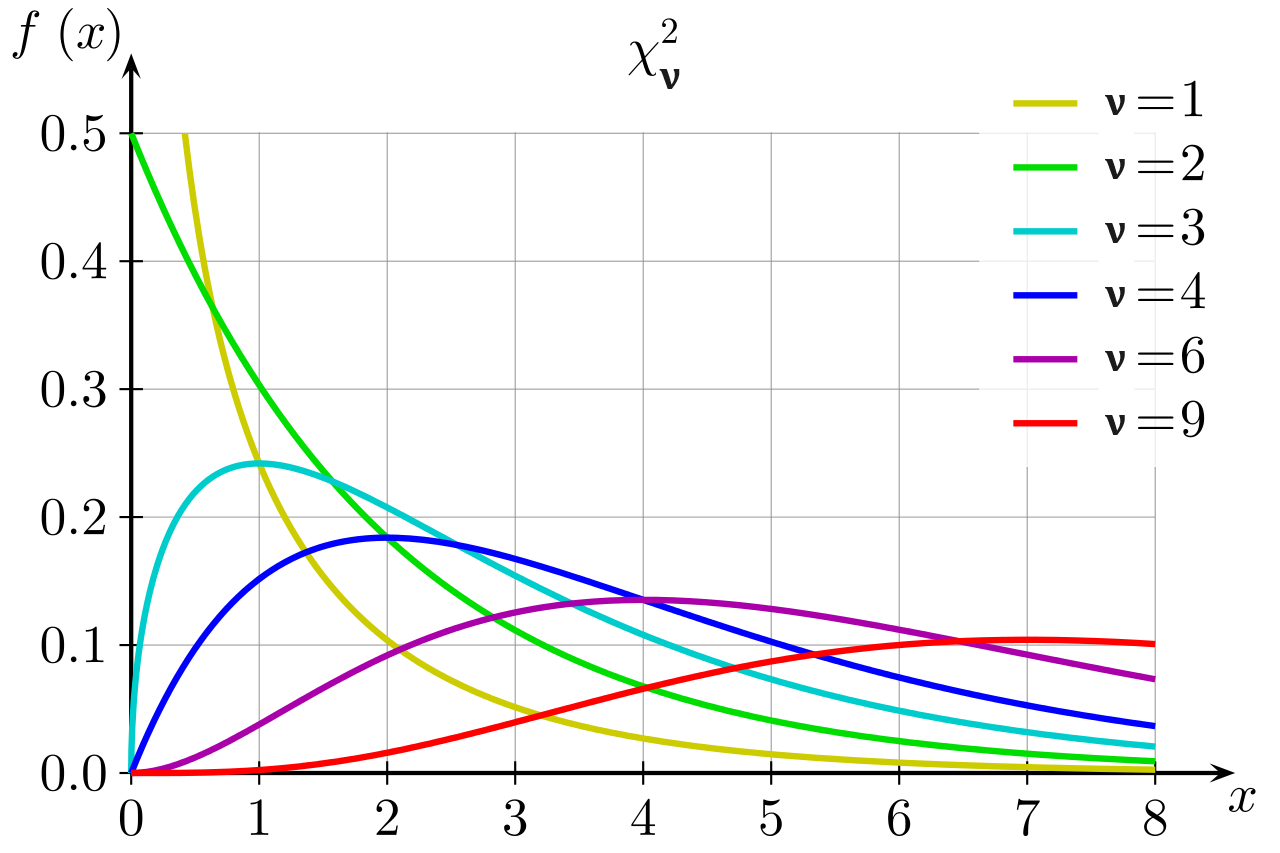
\includegraphics[width=0.5\textwidth]{figures/09-Contingency_table_binary_regression/Chi_square.png}
        \caption{卡方分配的機率密度函數,$\nu$ 代表卡方分配的自由度}
        \label{fig:chi_squared}
    \end{figure}

    由於卡方統計量取值越大,代表觀察值越偏離期望值,亦即資料越偏向對立假說,因此卡方適合度檢定的 $p$ 值應該取卡方分布右邊尾巴的機率,也就是 $\PP(\chi^2_{k-1} \ge X^2)$。同樣地,如果要用拒絕域法進行檢定,則拒絕域也會是右尾,因此在顯著水準為 $\alpha$ 的情況下,拒絕區為 $X^2 \ge \chi^2_{k-1, \alpha}$,其中 $\chi^2_{k-1, \alpha}$ 為 $\chi^2_{k-1}$ 右尾機率為 $\alpha$ 的臨界值。

    在上述的例子中,卡方統計量的取值為 $9.193$。計算 $p$ 值得到 $\PP(\chi^2_3 \ge 9.193) \approx 0.027$;另外,在顯著水準定為 $0.05$ 下,卡方統計量的拒絕域為 $X^2 \ge \chi^2_{3,0.05} \approx 7.81$。兩種方法都顯示,在顯著水準為 $0.05$ 下拒絕虛無假說,也就是這份問卷背後的母體族群教育程度分布顯著地異於全國教育程度之比例。

    \bigskip

    \begin{custom}{思考}
        當組數只有兩組時,若兩組人數觀察值分別為 $O_1$ 和 $O_2$,且我們想檢定第一組的母體比例是否為 $p_0$,此時適合度檢定的卡方檢定統計量為何?該檢定統計量和前面章節提到的單樣本比例檢定 $Z$ 統計量之間有什麼關係?
    \end{custom}
    
\section{雙因子列聯表、卡方同質性檢定與卡方獨立性檢定}

    在類別變項作為結果變項的分析中,我們也常想了解兩個類別變項之間是否有關係。此時我們可以將這兩個類別變項各種層次組合的發生次數紀錄於\textit{雙因子列聯表} (two-way contingency table) 中,例如表 \ref{tab:two_way_contingency_obs} 為我們的範例資料中「教育程度」與「衛教前願意篩檢」兩個類別變項的雙因子列聯表。為了後續符號化方便,我們把列聯表的row 數記為$r$、column 數記為 $c$、第 $i$ 個 row 第 $j$ 個 column 的觀察值記 $O_{ij}$、第 $i$ 個 row 的樣本數記為 $n_{i.}$、第 $j$ 個 column 的樣本數記為 $n_{.j}$、總樣本數記為 $n$。

    \begin{table}[htbp]
        \begin{center}
            \begin{tabular}{c|cccc|c}
                \toprule
                觀察值 & 碩博士 & 大專 & 高中職 & 國中以下 & 總和\\
                \hline
                衛教前願意篩檢 & 88 ($O_{11}$) & 402 ($O_{12}$) & 252 ($O_{13}$) & 162 ($O_{14}$) & 904 ($n_{1.}$)\\
                衛教前不願篩檢 & 50 ($O_{21}$) & 232 ($O_{22}$) & 207 ($O_{23}$) & 107 ($O_{24}$) & 596 ($n_{2.}$)\\
                \hline
                總和 & 138 ($n_{.1}$) & 634 ($n_{.2}$) & 459 ($n_{.3}$) & 269 ($n_{.3}$) & 1500 ($n$)\\
                \bottomrule
            \end{tabular}
            \caption{教育程度與衛教前篩檢意願的觀察值雙因子列聯表\label{tab:two_way_contingency_obs}}
        \end{center}
    \end{table}
    此時針對這兩個類別變項,我們有兩種可能的資料生成方式,與相對應的檢定:
    \begin{enumerate}
        \item 資料抽樣前其中一個變項各層次的觀察值數目已經固定。例如我們對六都居民的教育程度分佈差異有興趣,因此從台北市、新北市、桃園市、台中市、台南市、高雄市各隨機抽取了 300 位市民並調查每位市民的教育程度。此時如果針對「直轄市別」和「教育程度」作列聯表,則各個直轄市的總人數在抽樣前即已知而沒有變異性。這種情境下我們有興趣的問題是,各直轄市的教育程度分布是否不同。換句話說,我們想知道教育程度的分布在各直轄市之間是否\textit{同質} (homogeneity)。這類檢定被稱為 \textit{同質性檢定} (Test of homogeneity)。
        \item 兩個變項均為隨機抽樣。例如表 \ref{tab:two_way_contingency_obs} 中,我們在取得資料時並未對問卷填答者的衛教前篩檢意願及教育程度做任何篩選。這種情境下我們有興趣的問題是,「衛教前篩檢意願」和「教育程度」這兩個變項在資料中是否獨立。這類檢定被稱為 \textit{獨立性檢定} (Test of independence)。
    \end{enumerate}
    雖然上述兩種檢定在概念上略有不同,但實際進行檢定時,檢定統計量的計算方法與其虛無分佈均相同,因此這裡我們只針對獨立性檢定進行後續探討。獨立性檢定的虛無假說及對立假說分別為:
    \[\left\{\begin{array}{l}
        H_0: \text{表\ref{tab:two_way_contingency_obs}中每位填答者的衛教前篩檢意願和其教育程度獨立}\\
        H_1: \text{表\ref{tab:two_way_contingency_obs}中每位填答者的衛教前篩檢意願和其教育程度不獨立}
    \end{array} \right.\]
    而後我們參考配適度檢定的流程,試著算出虛無假說下每個格子的人數期望值。由於在虛無假說下篩檢意願和教育程度獨立,根據獨立的定義,資料中「碩博士且願意篩檢」的母體比例應等於「碩博士」的母體比例乘上「願意篩檢」的母體比例。然而此處我們不知道後面兩個母體比例,只能用資料下去估計:碩博士共有 $n_{.1} = 138$ 位,因此估計佔總體比例為 $n_{.1}/n = 138/1500$;願意篩檢者共有 $n_{1.} = 904$ 位,因此估計佔總體比例為 $n_{1.}/n = 904/1500$。因此,虛無假設下「碩博士且願意篩檢」的母體比例估計值為兩者相乘:$(n_{1.}/n)(n_{.1}/n) = (138/1500)(904/1500)$。最後,總樣本數乘上比例估計值即為「碩博士且願意篩檢」的人數期望值(我們記為 $E_{11}$):
    \[E_{11} = n \cdot \frac{n_{1.}}{n} \cdot \frac{n_{.1}}{n} = \frac{n_{1.}n_{.1}}{n} = \frac{904 \cdot 138}{1500} \approx 83.17\]
    同理,第 $i$ 個 row 第 $j$ 個 column 的人數期望值(記為 $E_{ij}$)可一般性地寫為該 row 樣本數($n_{i.}$)乘上該 column 樣本數($n_{.j}$)除以總樣本數:
    \[E_{ij} = \frac{n_{i.}n_{.j}}{n}\]
    將所有格子的期望值算出來後可以得到表\ref{tab:two_way_contingency_exp}。
    \begin{table}[htbp]
        \begin{center}
            \begin{tabular}{c|cccc|c}
                \toprule
                期望值 & 碩博士 & 大專 & 高中職 & 國中以下 & 總和\\
                \hline
                衛教前願意篩檢 & 83.17 ($E_{11}$) & 382.09 ($E_{12}$) & 276.62 ($E_{13}$) & 162.12 ($E_{14}$) & 904\\
                衛教前不願篩檢 & 54.83 ($E_{21}$) & 251.91 ($E_{22}$) & 182.38 ($E_{23}$) & 106.88 ($E_{24}$) & 596\\
                \hline
                總和 & 138 & 634 & 459 & 269 & 1500\\
                \bottomrule
            \end{tabular}
            \caption{教育程度與衛教前篩檢意願的期望值雙因子列聯表\label{tab:two_way_contingency_exp}}
        \end{center}
    \end{table}

    而後,我們參考適合度檢定的方法,將每個格子觀察值和期望值的差值平方,並以期望值標準化後加總,以建立卡方檢定統計量。差別只在於適合度檢定只有一個 row,而這裡我們有一整個矩陣要加總:
    \[X^2 = \sum_{i=1}^r \sum_{j=1}^c \frac{(O_{ij}-E_{ij})^2}{E_{ij}} = \frac{(88-83.17)^2}{83.17} + \frac{(402-382.09)^2}{382.09} + \cdots + \frac{(107-106.88)^2}{106.88} \approx 8.83\]
    在虛無假說下,當樣本數增加使得每個格子的期望值「夠大」時,$X^2$ 統計量的抽樣分布同樣會近似於卡方分布。我們可以思考一下該分布的自由度應該如何計算:首先我們總共有 $rc$ 個觀察值,但它們加總必須等於固定的總樣本數 $n$,因此總共有 $rc - 1$ 個可以自由變動的觀察值。但注意到我們在計算期望值時,用資料估計了兩個類別變項各階層的母體比例。在 row 代表的類別變項需要估計 $r-1$ 個母體比例(最後一個層次的比例用 $1$ 減去其他層次的比例即可),在 column 代表的類別變項則需要估計 $c-1$ 個母體比例。因此,卡方檢定量的虛無分佈自由度為「可以自由變動的觀察值數目」減去「用資料估計的參數個數」,即$(rc-1) - [(r-1) + (c-1)] = (r-1)(c-1)$。因此,一般性地來說,檢定兩個各有 $r$ 和 $c$ 個層次的類別變項是否獨立時,卡方獨立性檢定的統計量及虛無分布可寫為:
    \[X^2 = \sum_{i=1}^r \sum_{j=1}^c \frac{(O_{ij}-E_{ij})^2}{E_{ij}} \xrightarrow[]{d} \chi^2_{(r-1)(c-1)}\]

    和適合度檢定同理,卡方統計量取值越大,資料越偏向對立假說,因此卡方獨立性檢定的 $p$ 值也應該取右尾機率,也就是 $\PP(\chi^2_{(r-1)(c-1)} \ge X^2)$。如果用拒絕域法進行檢定,則拒絕域也會是右尾,因此在顯著水準為 $\alpha$ 的情況下,拒絕區為 $X^2 \ge \chi^2_{(r-1)(c-1), \alpha}$。在上述的例子中,卡方統計量的取值為 $8.83$,且其虛無分布近似於自由度等於 $(4-1)(2-1) = 3$ 的卡方分布。計算 $p$ 值得到 $\PP(\chi^2_3 \ge 8.83) \approx 0.032$;另外,在顯著水準定為 $0.05$ 下,卡方統計量的拒絕域為 $X^2 \ge \chi^2_{3,0.05} \approx 7.81$。兩種方法都顯示,在顯著水準為 $0.05$ 下拒絕虛無假說,也就是參加衛教的群體中,衛教前篩檢的意願和教育程度有顯著相關。

    卡方獨立性(同質性)檢定統計量之虛無分佈雖然可近似為 $\chi^2_{(r-1)(c-1)}$,但在兩個情境下該近似的效果較差:第一是當列聯表為 $2 \times 2$ 時,第二是當樣本數不夠多,以至於有格子的期望值在 $5$ 以下時。當列聯表為 $2 \times 2$ 時,可以考慮使用統計學家 Frank Yates (1902-1994) 提出的\textit{葉氏連續性校正} (Yates' continuity correction),將卡方統計量修改如下:
    \[X^2 = \sum_{i=1}^2 \sum_{j=1}^2 \frac{\max(|O_{ij}-E_{ij}|-0.5)^2,0)}{E_{ij}}\]
    可以看出,分子的部分當觀察值等於期望值時仍取值 $0$,當觀察值不等於期望值時則將差異往 $0$ 靠近 $0.5$ 後再平方。因此,葉氏連續性校正會讓卡方統計量變小,使檢定變得不容易顯著,以保持可接受的型一錯誤率。當有格子的期望值在 $5$ 以下時,則建議不再使用依賴於近似的卡方檢定,並改用\textit{費雪精確檢定} (Fisher's exact test)。費雪精確檢定是用資料的精確分佈來進行檢定,並不牽涉到近似,但其計算較複雜。幸運地是,當今的統計軟體均有提供費雪精確檢定,而且不需太多耗時即可完成計算。(事實上,依現在的電腦計算能力,任何獨立性或同質性檢定均可使用費雪精確檢定,不須限縮在格子的期望值於 $5$ 以下的情境。只是習慣上,當今研究還是在能用卡方檢定時就用卡方檢定。)費雪精確檢定的假說和結論解釋方法和卡方檢定相同,當$p$值在顯著水準以下時,代表拒絕「兩個類別變項之間獨立」的假說。
    
\section{成對類別資料與麥內瑪檢定}

    在表 \ref{tab:documentary_data} 的資料中,假設我們想知道衛教是否會影響參與者的篩檢意願。由於資料中沒有「衛教」這個變數,直覺上我們似乎可以把衛教前和衛教後的兩個變數轉置成如表 \ref{tab:dependent_data} 所示。如此我們便有兩個類別變項:衛教前後以及篩檢意願,如果這兩個二元變數不獨立,就代表衛教的確會影響篩檢意願。

    \begin{table}[htbp]
        \begin{center}
            \begin{tabular}{ccc}
                \toprule
                問卷編號 & 衛教前後 & 願意篩檢\\
                \hline
                1 & 前 & 是\\
                1 & 後 & 是\\
                2 & 前 & 否\\
                2 & 後 & 是\\
                3 & 前 & 是\\
                3 & 後 & 否\\
                4 & 前 & 是\\
                4 & 後 & 是\\
                5 & 前 & 否\\
                5 & 後 & 是\\
                6 & 前 & 否\\
                6 & 後 & 是\\
                $\vdots$ & $\vdots$ & $\vdots$\\
                \bottomrule
            \end{tabular}
            \caption{資料轉置後衛教前後和篩檢意願之資料表\label{tab:dependent_data}}
        \end{center}
    \end{table}

    為了進行卡方獨立性檢定,既定流程是將表 \ref{tab:dependent_data} 製作成雙因子列聯表並得到表 \ref{tab:mcnemar_table} 左側的表格。不過注意到,雖然我們的總樣本數只有 1500,但表 \ref{tab:mcnemar_table} 左側的總樣本數竟然有 3000!這是因為同一個人會貢獻兩筆資料,一筆是衛教前的篩檢意願、一筆是衛教後的篩檢意願,造成列聯表中四格的數字有隱含的相關性,因而違反了卡方獨立性檢定的基本假設。

    \begin{table}[htbp]
        \begin{center}
            \begin{tabular}{c|ccccc|cc}
                \cline{1-3}\cline{6-8}
                 & 願意篩檢 & 不願篩檢 &&& & 衛教後願意 & 衛教後不願意\\
                \cline{1-3}\cline{6-8}
                衛教前 & 1000 & 500 &&& 衛教前願意& 800 ($a$) & 200 ($b$)\\
                衛教後 & 1150 & 350 &&& 衛教前不願意& 350 ($c$) & 150 ($d$)\\
                \cline{1-3}\cline{6-8}
            \end{tabular}
            \caption{相依類別資料的列聯表\label{tab:mcnemar_table}}
        \end{center}
    \end{table}

    針對這個檢定問題,應該建立的列聯表如表 \ref{tab:mcnemar_table} 的右側所示,如此每位填答者僅會落在四個格子中的其中一格,因而消除了資料相依性的疑慮。在這裡我們看到,有 800 位填答者在衛教前後均願意接受篩檢、而有 150 位填答者則在衛教前後均不願接受篩檢。衛教對於這些人的意願均沒有影響,因此衛教若要能夠影響總體篩檢意願,必定來自於 (衛教前不願意, 衛教後願意) 與 (衛教前願意, 衛教後不願意) 這兩個格子。當前者的人數大於後者,則衛教後整體意願會提升;反之若前者的人數小於後者,則衛教後整體意願會下降。因此,我們可以只關注這兩個格子共 550 人,並將檢定問題轉化為:(衛教前不願意, 衛教後願意) 與 (衛教前願意, 衛教後不願意) 在這 550 人的母體比例是否相等?聰明的讀者可以發現,本檢定等價於預設兩組母體比例均為 0.5 的適合度檢定,因此其檢定統計量及虛無分布可寫為:
    \[X^2 = \frac{[b-(b+c)/2]^2}{(b+c)/2} + \frac{[c-(b+c)/2]^2}{(b+c)/2} = \frac{(b-c)^2}{b+c} \xrightarrow[]{d} \chi^2_1\]
    有些統計學家則建議此處亦使用葉氏連續性校正:
    \[X^2_{\text(Yates)} = \frac{[|b-(b+c)/2|-0.5]^2}{(b+c)/2} + \frac{[|c-(b+c)/2|-0.5]^2}{(b+c)/2} = \frac{(|b-c|-1)^2}{b+c} \xrightarrow[]{d} \chi^2_1\]
    $p$ 值與拒絕域的計算和適合度檢定相同:$p$ 值為 $\PP(\chi^2_1 \ge X^2)$,顯著水準為 $\alpha$ 的拒絕域則為 $X^2 \ge \chi^2_{1, \alpha}$。檢定結果拒絕虛無假說時,代表兩個變數之間的相關性顯著。此檢定由心理計量學家 Quinn McNemar (1900-1986) 所提出,因此被稱為\textit{麥內瑪檢定} (McNemar's test)。在我們的例子中,未使用葉氏連續性校正的卡方統計量為$(350-200)^2/(350+200) \approx 40.91$,而使用葉氏連續性校正的卡方統計量為$(|350-200|-1)^2/(350+200) \approx 40.37$,在顯著水準設定為 $0.05$下,兩者都遠超過拒絕域的臨界值 $\chi^2_{1,0.05} \approx 3.84$,代表拒絕虛無假說,衛教的確會顯著影響篩檢意願。而且,因為由不願意轉為願意的人比由願意轉為不願意的人多,所以衛教是顯著增加了篩檢意願。

\section{列聯表的變數相關性度量}
    我們現在知道如何用卡方檢定(以及麥內瑪檢定)來檢定兩個類別變數間的相關性。然而,檢定結果只能告訴我們兩者是否有顯著相關,而不能幫助我們評估相關性的強弱。讀者可能還記得,先前我們在探討兩個連續變數的相關性時,使用了皮爾森相關係數來量化相關性的強弱。然而,皮爾森相關係數運用在兩個類別變數時,有一個致命的缺點:在邊際機率 (marginal probability) 固定的強況下,皮爾森相關係數的取值範圍不再是 $-1$ 到 $1$。
    
    舉例而言,如表 \ref{tab:odds_ratio} 所示,左邊的表是觀察兩個二元變數 $X_1$ 和 $X_2$ 得到的結果,依照皮爾森相關係數的公式可以得到 $r=0.433$。這個數值看起來離 $1$ 還有點距離,因此 $X_1$ 和 $X_2$ 應該只有中度的相關性。但是我們可以思考:如果我們在收取資料前已知 $X_1$ 取值為 $1$ 的比例(又稱為 $X_1=1$ 的邊際機率)為 $\frac{100}{150}$、$X_2 = 1$ 取值為 $1$ 的比例(又稱為 $X_2=1$ 的邊際機率)為 $\frac{60}{150}$,那麼最終資料的皮爾森相關係數最大值會是多少?此時可以想像,為了要讓皮爾森相關係數最大化,我們希望 $(X_1, Y_1) = (1,1)$ 和 $(X_1, Y_1) = (0,0)$ 的人越多越好。因此,在維持各個 row 和 column 的總和不變的情況下,最大化皮爾森相關係數的資料應該形如表 \ref{tab:odds_ratio} 的右方所示,計算出的相關係數上限僅為 $r=0.577$。因此,我們觀察到的 $r=0.433$ 其實已經非常靠近上限。$X_1$ 和 $X_2$ 之間的相關性應當頗強,但是單看皮爾森相關係數的數值會讓我們誤認為它們之間僅有中度相關性。

    \bigskip

    \begin{table}[htbp]
        \begin{center}
            \begin{tabular}{c|cc|cccc|cc|c}
                \cline{1-4}\cline{7-10}
                觀察值 & $X_2=1$ & $X_2=0$ & 總和 &&& 極端值 & $X_2=1$ & $X_2=0$ & 總和\\
                \cline{1-4}\cline{7-10}
                $X_1=1$ & $55~(a)$ & $45~(b)$ & $100$ &&& $X_1=1$ & $60$ & $40$ & $100$\\
                $X_1=0$ & $5~(c)$ & $45~(d)$ & $50$ &&& $X_1=0$ & $0$ & $50$ & $50$\\
                \cline{1-4}\cline{7-10}
                總和 & $60$ & $90$ & $150$ &&& 總和 & $60$ & $90$ & $150$\\
                \cline{1-4}\cline{7-10}
            \end{tabular}
            \caption{$2 \times 2$列聯表以及皮爾森相關係數的上界\label{tab:odds_ratio}}
        \end{center}
    \end{table}

    為了對類別變數的相關性強度作更精緻、具有解釋意義的評估,流行病學家通常會用三種不同的效果度量 (effect measure):\textit{風險差} (risk difference)、\textit{風險比} (risk ratio)和\textit{勝算比} (odds ratio)。
    \begin{itemize}
        \item \textbf{風險差}:顧名思義為兩組\textit{風險} (risk)的差,即兩組事件發生機率的差。根據表\ref{tab:odds_ratio}的左側表格,如果我們有興趣的 outcome 是 $X_2$,其中 $X_2 = 1$ 代表發生事件,那麼$X_1 = 1$ 這組的風險是 $\frac{a}{a+b}$,$X_1 = 0$ 這組的風險則是 $\frac{c}{c+d}$。因此,兩組的風險差為 
        \[RD = \frac{a}{a+b}-\frac{c}{c+d}\]
        風險差大於 $0$ 代表 $X_1 = 1$ 這組的風險較高,反之亦然。風險差等於 $0$ 代表兩組的風險相等,換言之就是資料中 $X_1$ 和 $X_2$ 沒有相關。
        \item \textbf{風險比}:顧名思義為兩組風險的比值。由於歷史原因,風險比 (risk ratio) 也被稱為 \textit{相對風險} (relative risk),不過兩者的縮寫都是 RR,計算方法為
        \[RR = \frac{a}{a+b}\Big/\frac{c}{c+d} = \frac{a(c+d)}{c(a+b)}\]
        風險比大於 $1$ 代表 $X_1 = 1$ 這組的風險較高,反之亦然。風險比等於 $1$ 代表兩組的風險相等,也就是資料中 $X_1$ 和 $X_2$ 沒有相關。
        \item \textbf{勝算比}:顧名思義為兩組發生事件勝算 (odds) 的比值。我們在前面在篩檢工具的評估中有提到,勝算的定義為「事件發生的機率」除以「事件不發生的機率」,勝算較高也代表事件發生機率較高。因此,$X_1 = 1$ 這組的事件勝算為 $\frac{a}{b}$,$X_1 = 0$ 這組的事件勝算則是 $\frac{c}{d}$,而勝算比的計算方法為
        \[OR = \frac{a}{b}\Big/\frac{c}{d} = \frac{ad}{bc}\]
        可以看到勝算比的算法恰好是列聯表數據的「交叉相除」。勝算比大於 $1$ 代表 $X_1 = 1$ 這組的勝算較高,也就是事件機率較高,反之亦然。勝算比等於 $1$ 代表兩組的事件機率相等,也就是資料中 $X_1$ 和 $X_2$ 沒有相關。
    \end{itemize}
    就數字而言,以上三種效果度量都能量化兩個類比變項的相關程度,但它們的運用場合則取決於資料的收集方式。就實際應用上,風險比和風險差的目標是比較兩組的事件發生機率,較有直覺的解釋意義。然而,這個直覺解釋的前提是,資料中的各組事件發生機率能夠代表該組在母群體的事件發生機率。
    
    舉例來說,假定 $X_1$ 代表是否規律喝咖啡,$X_2$ 代表是否罹患胰臟癌。如果我們一開始從國民中抽取兩群人,一群有規律喝咖啡、一群沒有,並觀察他們十年內是否罹患胰臟癌,則資料裡 $X_1 = 1$ 這組中 $X_2 = 1$ 的比例即能代表規律喝咖啡者罹患胰臟癌的機率。然而,如果我們是一開始找一群罹患胰臟癌、及一群未罹患胰臟癌的人,並反向詢問他們十年內的喝咖啡習慣,那麼資料裡 $X_1 = 1$ 這組中 $X_2 = 1$ 的比例就 \textbf{無法} 代表規律喝咖啡者罹患胰臟癌的機率。前面這種研究設計被稱為\textit{世代研究} (cohort study),可以使用風險比或風險差來量化。後面這種研究設計被稱為\textit{病例對照研究} (case-control study),此時各組的風險沒有直覺的解釋意義,所以通常僅會用勝算比來量化兩者的相關性。

    一個較特別的情況是成對類別資料。我們在前一節提到,這種類型的資料需要將資料按照觀察值的配對關係建立列聯表,例如表 \ref{tab:mcnemar_table} 的右側表格所示。我們在麥內瑪檢定中提到,表格中左上$(a)$和右下$(d)$的格子並未提供關於衛教和篩檢意願的相關性資訊,所以在計算兩個類別變數的相關性指標時,也不應用到這兩個數值。這類配對的列聯表通常使用\textbf{勝算比}作為相關性指標,且計算方法為恰好為剩下的兩格相除:
    \[OR = \frac{b}{c}\]
    此處的勝算比算法,依照表 \ref{tab:mcnemar_table} 的資訊,因為 $b>c$ 隱含(在衛教前後篩檢意願不同的人中)衛教前願意的人比衛教後願意的人多,因此代表「衛教前相對於衛教後,願意篩檢的勝算比」。如果該勝算比大於 $1$,代表衛教和篩檢意願降低有關;反之,如果該勝算比小於 $1$,代表衛教和篩檢意願增加有關。

\section{二元回歸}

    前面我們討論的列聯表分析,可以用以評估兩個類別變項之間的關係。然而,在實際分析中也很常出現的狀況是,我們有興趣的結果變數仍是二元變數,但預測變數是連續變數、或預測變數有兩個以上。此時我們不再能單純使用列聯表分析及卡方檢定來評估變數之間的相關性,不過我們可以從上一章的線性回歸模型找靈感,試著建立以二元變數為反應變數的\textit{二元回歸} (binary regression)。在簡單線性回歸中,我們對模型的假設為
    \[Y = \beta_0 + \beta_1 X + \varepsilon, \qquad \varepsilon \sim \NN(0,\sigma^2)\]
    上面的模型也可以拆開寫成
    \begin{gather*}
        Y|X \sim \NN(\mu, \sigma^2)\\
        \mu := \EE[Y|X] = \beta_0 + \beta_1 X
    \end{gather*}
    第一行代表給定預測變數 $X$ 後,反應變數 $Y$ 呈現一個期望值等於 $\mu$、變異數為 $\sigma^2$ 的常態分布。第二行則說該期望值 $\mu$ 跟 $X$ 呈現線性關係。當 $Y$ 為一個二元變數時,我們無法直接套用簡單線性回歸,因為它的模型假設有許多地方不符合預期。首先,$Y$ 為一個二元變數,所以給定 $X$ 後,$Y$ 不會服從一個常態分布,而是應該服從一個白努利分布。白努利分布的機率參數 $p$ 恰為其期望值,所以我們可以將第二行的 $\mu$ 用 $p$ 取代並得到
    \begin{gather*}
        Y|X \sim \text{Bernoulli}(p)\\
        p := \EE[Y|X] = \beta_0 + \beta_1 X
    \end{gather*}
    雖然我們把 $Y$ 的條件分布矯正了,這個新模型還是有一處不合適:第二行的左手邊是 $p$,代表事件發生的機率,因此其取值應該介於 $0$ 和 $1$ 之間。但是第二行的右手邊則沒有取值的限制,不但可能超過 $1$,還有可能是負的。換句話說,在這個模型下,根據各觀察值的 $X$ 取值,我們可能會預測其事件發生機率大於一或小於零!

    為了避免上述不合實際的預測值,我們在進行二元回歸時,不會直接假定事件發生機率 $p$ 和解釋變數 $X$ 呈現線性關係,而是假定 $p$ 的某個函數和解釋變數 $X$ 呈現線性關係。這個函數被稱為連結函數 (link function),它的目的是要把取值區間為 $[0,1]$ 的機率 $p$ 轉換成取值區間為 $(-\infty, \infty)$ 的 $\beta_0 + \beta_1 X$。其中生物醫學研究最常使用的連結函數為\textit{羅吉函數} (logit function),$\text{logit}(x) = \log\big(\frac{x}{1-x}\big)$,其中 $\log$ 為自然對數(讀者可以自行驗證該函數是否可以正確進行上述的取值區間轉換)。將羅吉函數帶入我們上面的模型即可得到
    \begin{gather*}
        Y|X \sim \text{Bernoulli}(p)\\
        \log\Big(\frac{p}{1-p}\Big) = \beta_0 + \beta_1 X
    \end{gather*}
    第二行等號左側的 $\log\big(\frac{p}{1-p}\big)$ 恰為事件勝算 $\frac{p}{1-p}$ 取自然對數,即\textit{對數勝算} (log odds)。這個模型因為使用了羅吉函數當作連結函數,而且解釋變數只有一個,因此被稱為\textit{簡單羅吉斯回歸} (simple logistic regression)。
        
    和簡單線性回歸一樣,我們通常有興趣的是 $X$ 的回歸係數 $\beta_1$:$X$ 的值每增加 $1$,對數勝算會增加 $\beta_1$。根據這個結果,如果原本的事件勝算為 $a$、對數勝算為 $\log a$,則 $X$ 的值增加 $1$ 後,對數勝算會變成 $\beta_1 + \log a$、事件勝算會變成 $e^{\beta_1 + \log a} = ae^{\beta_1}$。換句話說,$X$ 的值每增加 $1$,$Y$ 事件勝算就變為 $e^{\beta_1}$ 倍,所以 $e^{\beta_1}$ 常被稱為 $X$ 相對於 $Y$ 的\textit{勝算比} (odds ratio),而 $\beta_1$ 則被稱為\textit{對數勝算比} (log odds ratio) 。當勝算比大於 $1$、也就是對數勝算比大於 $0$ 時,隨著 $X$ 增加, $Y$ 事件機率也增加;當勝算比小於 $1$、也就是對數勝算比小於 $0$ 時,隨著 $X$ 增加, $Y$ 事件機率則降低。因此,我們在判斷 $X$ 與 $Y$ 是否有關時,即欲檢定勝算比 $e^{\beta_1}$ 是否等於 $1$,或對數勝算比 $\beta_1$ 是否等於 $0$。

    針對回歸係數 $\beta_1$ 的估計與檢定,其原理和簡單線性回歸類似,但過程有些許不同。首先,$\beta_1$ 常用的估計方式不是最小平方法,而是需要演算法迭代的最大概似法 (maximum likelihood estimator)。根據統計理論的推導,在\textbf{樣本數夠大}的情況下,最大概似法得出的估計值 $\hat{\beta}_1$ 之抽樣分布近似於常態分布,且其標準誤亦可從資料中估出,我們記為 $\widehat{se}(\hat{\beta}_1)$。因此,類似簡單線性回歸,如果要檢定 $\beta_1 = 0$,也就是 $X$ 和 $Y$ 之間無關的虛無假設,我們的檢定統計量為 $\frac{\hat{\beta}_1}{\widehat{se}(\hat{\beta}_1)}$,且其虛無分布近似為標準常態分布。另外,$\beta_1$ 的雙尾 $(1-\alpha)\times 100\%$ 近似信賴區間可寫為:
    \[(\hat{\beta}_1 - z_{\alpha/2} \widehat{se}(\hat{\beta}_1), \;\; \hat{\beta}_1 + z_{\alpha/2} \widehat{se}(\hat{\beta}_1))\]
    然而大多數時候,為了判讀方便,研究中常不會選擇報告對數勝算比 $\beta_1$ 的信賴區間,而是會報告勝算比 $e^{\beta_1}$ 的信賴區間。此時只要把 $\beta_1$ 的信賴區間上下界取自然指數即可:
    \[(e^{\hat{\beta}_1 - z_{\alpha/2} \widehat{se}(\hat{\beta}_1)}, \;\; e^{\hat{\beta}_1 + z_{\alpha/2} \widehat{se}(\hat{\beta}_1)})\]
    勝算比的信賴區間也常被拿來判斷 $X$ 和 $Y$ 是否相關。在顯著水準為 $\alpha$ 下,如果該區間沒有蓋到 $1$(即「無相關」隱含的勝算比數值),則代表 $X$ 和 $Y$ 有統計顯著的相關。反之,則沒有足夠證據顯示 $X$ 和 $Y$ 有相關。

    在線性回歸中,我們將解釋變數拓展到兩個以上,並假設反應變數與解釋變數的關係仍為線性後,就得到多重線性回歸。同理,在羅吉斯回歸中,我們也可以將解釋變數增加到兩個以上,以得到如下的 \textit{多重羅吉斯回歸} (multiple logistic regression)模型。
    \begin{gather*}
        Y|X \sim \text{Bernoulli}(p)\\
        \log\Big(\frac{p}{1-p}\Big) = \beta_0 + \beta_1 X_1 + \beta_2 X_2 + ... + \beta_q X_q
    \end{gather*}
    其中回歸係數的解釋和多重線性回歸類似。以 $\beta_1$ 為例,其代表 \textbf{控制 $X_2, X_3,...,X_q$ 不變的情況下},$X_1$ 每增加一單位,$Y$ 事件對數勝算的增加量,或簡稱為 $X_1$ 相對於 $Y$ 事件的對數勝算比。而 $e^{\beta_1}$ 則是控制其他解釋變數不變的情況下,$X_1$ 相對於 $Y$ 事件的勝算比,也常被稱為 $X_1$ 相對 $Y$ 事件的\textit{調整勝算比} (adjusted odds ratio)。

    \bigskip

    \begin{custom}{練習}
        某研究欲了解,針對院外心跳停止接受心肺復甦並恢復自發循環的病患,有那些預測因子可預測其離開加護病房後神經學表現的好壞。研究者以神經學表現好(1)與壞(0)作為反應變數,對年齡、糖尿病史、阻塞性肺病史、癌症史、心跳停止時是否有旁人協助心肺復甦、到院時心律、心肺復甦時給予的腎上腺素劑量與恢復自發循環時的舒張壓建立多重羅吉斯回歸模型。模型估計後得到「心跳停止時有旁人協助心肺復甦」的迴歸係數與標準誤估計值為 $0.800 \pm 0.297$。請 (1) 解釋上述估計值的意義 (2) 給出「心跳停止時有旁人協助心肺復甦」相對於「離開加護病房後神經學表現好壞」的調整勝算比估計值 (3) 給出該調整勝算比的 $95\%$ 雙尾信賴區間 (4) 根據該區間,在顯著水準為 $0.05$ 下,檢定調整其他變數後,「心跳停止時有旁人協助心肺復甦」是否會影響「離開加護病房後神經學表現好壞」。
    \end{custom}
    
    \begin{docexam}{(107-2醫學(二))}
        病例對照研究中,吸菸對口腔癌發生之勝算比值 (odds ratio) 為 2.0 倍。若健康對照個案之中有 25\% 個案吸菸,則 400 名罹患口腔癌病患之中有多少名病患吸菸?
    \end{docexam}
    
    \begin{docexam}{(107-1醫學(二))}
        某研究者想探討酒駕與死亡車禍的關係,所以在某縣市統計半年的車禍資料,將車禍分為是否有人員 24 小時內死亡,並調查每次車禍中開車者是否有酒駕行為,下列統計方法何者最恰當?

        (A) 線性回歸 (Linear regression)
        
        (B) 獨立樣本 $t$ 檢定 (Independent sample $t$-test)

        (C) 配對 $t$ 檢定 (Paired $t$-test)
 
        (D) 卡方檢定 (Chi-squared test)
    \end{docexam}
    
    \begin{docexam}{(106-2醫學(二))}
        為研究大腸癌病人術前準備情況與術後併發症的關係,某研究收集 6 位術前準備情況較好之大腸癌病人與 4 位術前準備情況較差者,術後兩組發生併發症的人數分別為 1 位與 3 位。下列何種統計方法最恰當?

        (A) 費雪恰當檢定 (Fisher's exact test)
        
        (B) 獨立樣本 $t$ 檢定 (Independent sample $t$-test)

        (C) 卡方檢定 (Chi-squared test)
 
        (D) McNemar 檢定 (McNemar's test)
    \end{docexam}
    
    \begin{docexam}{(106-2醫學(二))}
        假設我們要比較兩種抗生素 A 和 B 治療淋病的效果,接受抗生素 A 的病人必須和接受抗生素 B 的病人經過年齡和性別的配對,這些病人必須在一星期之內回到診所內,檢查淋病是否已經被消除。假設結果如下:

        \begin{enumerate}[(a)]
            \item 有 40 對抗生素 A 和 B 的配對病人,淋病都已經被消除;
            \item 有 20 對的配對病人,抗生素 A 消除淋病,但抗生素 B 無效;
            \item 有 16 對的配對病人,抗生素 A 無效,但抗生素 B 消除淋病;
            \item 有 3 對的配對病人,抗生素 A 和 B 都無法消除淋病;
        \end{enumerate}

        你將採用何種統計方法檢定上述資料?

        (A) 兩個樣本 $t$ 檢定
        
        (B) 卡方檢定

        (C) 配對 $t$ 檢定
 
        (D) 麥內瑪檢定 (McNemar's test)
    \end{docexam}
    
    \begin{docexam}{(105-1醫學(一))}
        在進行卡方檢定時,若有某一個細格之預期值小於或等於 5,則須選用何種統計方法較為適當?

        (A) 簡單回歸分析 (simple regression)
        
        (B) 多變項分析 (multivariate analysis)

        (C) 變異量分析 (analysis of variance)
 
        (D) 費雪恰當檢定 (Fisher's exact test)
    \end{docexam}
    
    \begin{docexam}{(103-2醫學(一))}
        根據肺癌病例對照研究結果,100 名肺癌患者中 90 名有抽菸,100 名健康者中有 50 名有抽菸,則抽菸引起肺癌的勝算比 (odds ratio) 為?
    \end{docexam}
    
    \begin{docexam}{(103-2醫學(一))}
        比較兩組病人某項檢查陽性的比例 (proportions)可使用下列何種統計方法?
        
        (A) 卡方檢定 (Chi-squared test)
        
        (B) $t$ 檢定 (Student's t test)

        (C) 曼惠特尼檢定 (Mann-Whitney test)
 
        (D) 變異數分析 (ANOVA)
    \end{docexam}
    
    \begin{docexam}{(103-1醫學(一))}
        探討貧窮與兒童肥胖之間的關係,若非貧窮兒童的肥胖率為 20\%,貧窮兒童的肥胖率為 40\%,下列敘述何者正確?
        
        (A) 貧窮是肥胖的危險因子,相對危險比 (relative risk) 為 2
        
        (B) 貧窮是肥胖的危險因子,相對危險比 (relative risk) 為 1/2

        (C) 貧窮是肥胖的保護因子,相對危險比 (relative risk) 為 2
 
        (D) 貧窮是肥胖的保護因子,相對危險比 (relative risk) 為 1/2
    \end{docexam}
    
    \begin{docexam}{(106-2醫學(二))}
        一個臨床試驗評估密集運動計畫擬探討初次發病存活至少 30 天的心肌梗塞病人的有效性,初次發病存活至少 30 天的心肌梗塞病人被隨機分配至密集運動計畫或一般照護 (usual care)。在 100 名一般照護的病人中,30 名病人在三年的追蹤期間死亡;在 100 名密集運動計畫的病人中,50 名病人在三年的追蹤期間死亡。密集運動計畫組相較於一般照護組的死亡相對危險性 (relative risk of death)為何?
    \end{docexam}
    
    \begin{docexam}{(101-2醫學(一))}
        某 case-control study 研究某基因型與乳癌的關係,將基因型分為 GG+GT 與 TT 兩類,計算得知 GG+GT 組比 TT 組的勝算比 (odds ratio) 為 $2.4$,95\% 信賴區間(95\% confidence interval) 為 $(1.4, 4.3)$。下列何者正確?
        
        (A) 具 GG+GT 基因型較 TT 型易發生乳癌,有統計上顯著意義
        
        (B) 具 GG+GT 基因型較 TT 型不易發生乳癌,有統計上顯著意義

        (C) 具 GG+GT 基因型較 TT 型易發生乳癌,沒有統計上顯著意義
 
        (D) 具 GG+GT 基因型較 TT 型不易發生乳癌,沒有統計上顯著意義
    \end{docexam}
    
    \begin{docexam}{(101-1醫學(一))}
        某大型臨床試驗研究每日服用低劑量 Aspirin 藥物與日後發生心肌梗塞的關係。隨機分配 10000 人到 Aspirin 組,另外分配 10000 人到安慰劑組 (placebo)。追蹤一段時間後 Aspirin 組有 100 人發生心肌梗塞,安慰劑組有 180 人發生心肌梗塞。下列何者錯誤?
        
        (A) Aspirin 組比安慰劑組的相對風險比 (relative risk) 大於 1
        
        (B) 可採 Chi-squared test 檢定服用 Aspirin 是否與得心肌梗塞有關

        (C) 可採 Fisher exact test 檢定服用 Aspirin 是否與得心肌梗塞有關
 
        (D) 可採 Two-sample z test 檢定服用 Aspirin 是否與得心肌梗塞有關
    \end{docexam}
    
    \begin{docexam}{(100-2醫學(一))}
        假設 10 年前 25\% 的心肌梗塞病人在發病 24 小時內死亡,這個比例稱為個案致死率 (case fatality),有位研究者想了解這 10 年來心肌梗塞病人的個案致死率是否有顯著的改變,在他收集的 15 位新的心肌梗塞病人,5 位 24 小時內死亡,此研究者應該使用何種統計方法來回答他的研究問題?
        
        (A) 單一樣本 $Z$ 檢定
        
        (B) 單一樣本 $t$ 檢定

        (C) 單一樣本二項比例檢定
 
        (D) 兩個樣本二項比例檢定
    \end{docexam}
    
    \begin{docexam}{(110-2醫學(二))}
        為檢定機器人輔助式 (robot-assisted) 手術與傳統手術於術後發生併發症之關聯,收集 10 位接受機器人輔助式手術及 12 位進行傳統手術病人的資料,兩種手術發生術後併發症人數分別為 1、2 人。應該採用下列何者統計方法分析最恰當?
        
        (A) 簡單線性回歸分析 (Simple linear regression)
        
        (B) 對數等級檢定 (Log rank test)

        (C) 卡方檢定 (Chi-squared test)
 
        (D) 費雪恰當檢定 (Fisher's exact test)
    \end{docexam}
    
    \begin{docexam}{(109-1醫學(二))}
        某研究者想檢定某基因多型性(AA/AG 組相對於 GG 組)是否與口腔癌的發生有關,在某醫院有 200 名口腔癌患者參與此研究,每位口腔癌患者都配對 1 名沒有口腔癌的健康者,分別測量其基因型,下列統計分析方法何者最恰當?
        
        (A) 線性回歸
        
        (B) 獨立樣本之卡方檢定

        (C) 配對 $t$ 檢定
 
        (D) McNemar 卡方檢定
    \end{docexam}
    
    \begin{docexam}{(109-2醫學(二))}
        處理 $2 \times 2$ 列聯表數據之統計分析,若其中一個細格的期望值小於 5,此時應使用下列何種方法執行統計學檢定較為恰當?
        
        (A) 卡方檢定 (Chi-squared test)
        
        (B) 費雪恰當檢定 (Fisher's exact test)

        (C) Yates校正之卡方檢定法 (Yates correction Chi-squared test)
 
        (D) McNemar檢定法 (McNemar Chi-squared test)
    \end{docexam}
    
    \begin{docexam}{(108-2醫學(二))}
        某病例對照研究 (case-control study) 研究吸菸與某疾病之關係,資料如以下列聯表:
        \begin{table}[htbp]
            \begin{center}
                \begin{tabular}{c|cc|c}
                    & 吸菸 & 不吸菸 & \\
                    \hline
                    病例 & 5 & 45 & 50\\
                    對照 & 3 & 47 & 50\\
                    \hline
                    & 8 & 92 & 100
                \end{tabular}
            \end{center}
        \end{table}
        
        \noindent 若要就吸菸與得該疾病的關係做統計檢定,下列何種方法最適當?
        
        (A) 獨立 $t$ 檢定 (two-sample $t$-test)
        
        (B) 配對 $t$ 檢定 (paired $t$-test)

        (C) McNemar 卡方檢定 (McNemar Chi-squared test)
 
        (D) 費雪恰當檢定 (Fisher's exact test)
    \end{docexam}

\nocite{*} 
% \appendix
% \chapter{線性代數}

\section{線性代數}

\subsection{橫向量、縱向量}
線性代數,而且能讓。

橫向量(row vector, 大陸稱為行向量、台灣稱為列向量)
\[\begin{bmatrix} 1 & 2 & 3 \end{bmatrix}\]

縱向量(column vector, 大陸稱為列向量、台灣稱為行向量)
\[\begin{bmatrix} 
    1 \\ 
    2 \\ 
    3 
  \end{bmatrix}\]
    
向量內積
\[\begin{bmatrix} 
    u_1 & u_2 & \cdots & u_k 
  \end{bmatrix}\begin{bmatrix} 
    v_1 \\
    v_2 \\
    \vdots \\
    v_k 
  \end{bmatrix} = u_1v_1 + u_2v_2 + \cdots + u_kv_k\]
  
向量外積
\[\begin{bmatrix} 
    u_1 \\
    u_2 \\
    \vdots \\
    u_k 
  \end{bmatrix}\begin{bmatrix} 
    v_1 & v_2 & \cdots & v_k 
  \end{bmatrix} = \begin{bmatrix}
    u_1v_1 & u_1v_2 & \cdots & u_1v_k\\
    u_2v_1 & u_2v_2 & \cdots & u_2v_k\\
    \vdots & \vdots & \ddots & \vdots\\
    u_kv_1 & u_kv_2 & \cdots & u_kv_k\end{bmatrix}\]

\begin{note}
haha
\end{note}

% \bibliography{reference}

\end{document}
